%% ----------------------------------------
%%
%% NYU PhD thesis template.
%% Created by José Koiller 2007--2008.
%% Modified by Siddharth Krishna, 2019.
%%
%% ----------------------------------------


%% Use the first of the following lines during production to
%% easily spot "overfull boxes" in the output. Use the second
%% line for the final version.
%\documentclass[12pt,draft,letterpaper]{report}
\documentclass[12pt,oneside,letterpaper]{report}


% ----------------------------------------
% Macro to switch between draft version and final version
% ----------------------------------------

% Use or comment this to enable/disable draft version
% \def\draftversion{}
\newcommand{\draftfinal}[2]{\ifdefined\draftversion#1\else#2\fi}
\newcommand{\draftonly}[1]{\draftfinal{#1}{}}
\newcommand{\finalonly}[1]{\draftfinal{}{#1}}


% ----------------------------------------
% Thesis metadata
% ----------------------------------------

%% Replace the title, name, advisor name, graduation date and dedication below
%% with your own. Graduation months must be January, May or September.
\newcommand{\thesistitle}{Data Science Methods for Large-Scale Structure Cosmology}
\newcommand{\thesisauthor}{Kate Storey-Fisher}
\newcommand{\thesisadvisor}{Professor David W. Hogg}
\newcommand{\thesisdept}{Physics}
\newcommand{\gradmonth}{September}
\newcommand{\gradyear}{2023}
%% If you do not want a dedication, scroll down and comment out
%% the appropriate lines in this file.
\newcommand{\thesisdedication}{[Dedication]}


% ----------------------------------------
% Layout and formatting
% ----------------------------------------

% Uncomment to get a big black box to spot "overfull hboxes"
% \setlength{\overfullrule}{5pt}


%% Page layout (customized to letter paper and NYU requirements):
\RequirePackage[margin=1in, includefoot, letterpaper]{geometry}


%% Color definitions:
\RequirePackage[prologue]{xcolor}
\definecolor[named]{ThesisBlue}{cmyk}{1,0.1,0,0.1}
\definecolor[named]{ThesisYellow}{cmyk}{0,0.16,1,0}
\definecolor[named]{ThesisOrange}{cmyk}{0,0.42,1,0.01}
\definecolor[named]{ThesisRed}{cmyk}{0,0.90,0.86,0}
\definecolor[named]{ThesisLightBlue}{cmyk}{0.49,0.01,0,0}
\definecolor[named]{ThesisGreen}{cmyk}{0.20,0,1,0.19}
\definecolor[named]{ThesisPurple}{cmyk}{0.55,1,0,0.15}
\definecolor[named]{ThesisDarkBlue}{cmyk}{1,0.58,0,0.21}

% School color found from university's graphic identity site:
% http://www.nyu.edu/employees/resources-and-services/media-and-communications/styleguide.html
\definecolor{SchoolColor}{rgb}{0.3412, 0.0235, 0.5490} % purple
\definecolor{chaptergrey}{rgb}{0.2600, 0.0200, 0.4600} % dialed back a little
\definecolor{midgrey}{rgb}{0.4, 0.4, 0.4}
\definecolor{darkgrey}{rgb}{0.25, 0.25, 0.25}
\definecolor{mulberry}{HTML}{A93C93}

\usepackage{hyperref}
\hypersetup{colorlinks,
  linkcolor=darkgrey,
  citecolor=mulberry,
  urlcolor=mulberry,
  filecolor=mulberry}


%% Captions of Figures, tables
\RequirePackage[labelfont={bf,sf,small,singlespacing},
                textfont={sf,small,singlespacing},
                % justification={justified,RaggedRight},
                % singlelinecheck=false,
                margin=0pt,
                figurewithin=chapter,
                tablewithin=chapter]{caption}

%% Chapter headings, captions
\usepackage{fix-cm}
\RequirePackage[raggedright,sc]{titlesec}
\definecolor{gray75}{gray}{0.75}
\newcommand{\hsp}{\hspace{20pt}}

\titleformat{\chapter}[hang]
{\Huge\sc}
{\textcolor{black}{\thechapter}\hsp\textcolor{gray75}{|}\hsp}
{0pt}{\Huge\sc\raggedright}
% [\textcolor{gray75}{|}\hsp\textcolor{SchoolColor}{\thechapter}]


%% The following makes chapters and sections, but not subsections,
%% appear in the TOC (table of contents). Increase to 2 or 3 to
%% make subsections or subsubsections appear, respectively. It seems
%% to be usual to use the "1" setting, however.
\setcounter{tocdepth}{1}

%% Sectional units up to subsubsections are numbered. To number
%% subsections, but not subsubsections, decrease this counter to 2.
\setcounter{secnumdepth}{3}


%% Use the following commands, if desired, during production.
%% Comment them out for final version.
%\usepackage{layout} % defines the \layout command, see below
%\setlength{\hoffset}{-.75in} % creates a large right margin for notes and \showlabels

%% Controls spacing between lines (\doublespacing, \onehalfspacing, etc.):
\usepackage{setspace}

%% Use the line below for official NYU version, which requires
%% double line spacing. For all other uses, this is unnecessary,
%% so the line can be commented out.
\finalonly{
  \doublespacing % requires package setspace, invoked above
}

%% For generating sample text.
%% Can be removed when you've replaced all \lipsum commands with your text.
\usepackage{lipsum}


% ----------------------------------------
% Comments and TODOs:
% ----------------------------------------

% Uncomment this to remove all comments
\newcommand{\nocomments}{}

% Uncomment this to remove all TODOs
\newcommand{\notodos}{}

% Comments and TODOs
\newcommand{\fcomment}[2]{\ifdefined\nocomments{}\else\footnote{\textcolor{red}{#1:} #2}\fi}
\newcommand{\todo}[1]{\ifdefined\notodos{}\else\textcolor{red}{TODO\ifstrempty{#1}{}{: #1}}\fi}
\newcommand{\ftodo}[1]{\ifdefined\notodos{}\else\fcomment{TODO}{#1}\fi}

% Author comments:
\newcommand{\aen}[1]{\fcomment{Emmy}{#1}}


% ----------------------------------------
% User-specific packages and macros
% ----------------------------------------

%% This inputs your auxiliary file with \usepackage's and \newcommand's:
%% It is assumed that that file is called "defs.tex".
%% not using template; in sections. should pull out into defs files probs
% ----------------------------------------
% Packages
% ----------------------------------------

% 
% Place here your \usepackage's. Some recommended packages are already included.
%

% Graphics:
\usepackage[final]{graphicx}
%\usepackage{graphicx} % use this line instead of the above to suppress graphics in draft copies
%\usepackage{graphpap} % \defines the \graphpaper command

% Uncomment this to indent first line of each section:
% \usepackage{indentfirst}

% Good AMS stuff:
\usepackage{amsthm} % facilities for theorem-like environments
%\usepackage[tbtags]{amsmath} % a lot of good stuff!
\usepackage{amsmath} % a lot of good stuff!
\usepackage{mathtools}


% Fonts and symbols:
\usepackage{amsfonts}
\usepackage{amssymb}

% Set the fonts
\RequirePackage[T1]{fontenc}
\ifxetex
  \RequirePackage[tt=false]{libertine}
\else
  \RequirePackage[tt=false, type1=true]{libertine}
\fi
\RequirePackage[varqu]{zi4}
\RequirePackage[libertine]{newtxmath}


% For typesetting inference rules
\usepackage{mathpartir}
% \usepackage{pftools}  % A local package
\newcommand{\bmmax}{2}
\usepackage{bm}

% Formatting tools:
%\usepackage{relsize} % relative font size selection, provides commands \textsmalle, \textlarger
\usepackage{xspace} % gentle spacing in macros, such as \newcommand{\acims}{\textsc{acim}s\xspace}


\usepackage[T1]{fontenc} % needed for scaling fancy fonts (?)
\usepackage[utf8]{inputenc} % not sure this is needed

% To stop citations overflowing lines
\usepackage{breakcites}

% For citet command
\usepackage{natbib}
% \setcitestyle{%
%     authoryear,%
%     open={[},close={]},citesep={;},%
%     aysep={},yysep={,},%
%     notesep={, }}
% \let\cite\citep


%%%% MACROS %%%%%

%%%% general %%%%%

% anomalies uses subcaption and aemulus uses subfig.
% they don't play together. gonna have to update anomalies to subfig, best option i think
%\usepackage{subcaption}
\usepackage[caption=false]{subfig}
\usepackage{bm}		% Bold maths symbols, including upright Greek
\usepackage{verbatim}

% misc
\newcommand{\documentname}{\textsl{Article}\xspace}
\newcommand{\eqt}[1]{equation~(\ref{#1})}

% units
\newcommand{\hmpc}{$h^{-1}\,$Mpc}
\newcommand{\hMpc}{h\inv\,\mathrm{Mpc}\xspace}
\newcommand{\hGpc}{h\inv\,\mathrm{Gpc}\xspace}
\newcommand{\Mpch}{h\,\mathrm{Mpc}\inv\xspace}
\newcommand{\Msun}{M_\mathrm{\odot}\xspace}
\newcommand{\hMsun}{h\inv M_\mathrm{\odot}\xspace}

% math
\newcommand{\inv}{^{-1}}
\newcommand{\invp}{^{'-1}}
\newcommand{\T}{^{\mathsf{T}}}
\newcommand{\Tp}{^{'\mathsf{T}}}

% edits
%\newcommand{\new}[1]{\textbf{#1}} % Bolded revisions
\newcommand{\new}[1]{#1} % Un-bold revisions after final acceptance


% comments
\newcommand{\KSF}[1]{\textcolor{teal}{KSF says: #1}}
\newcommand{\ksf}[1]{{\color{teal}KSF says: #1}}
\newcommand{\hogg}[1]{\textcolor{red}{Hogg says: #1}}
%\newcommand{\new}[1]{\textbf{#1}}
%\newcommand{\new}[1]{#1}

% style
\newcommand{\bld}[1]{\bm{#1}}
\urlstyle{tt}

%%%%% Chapter: CFE %%%%%

% language
\newcommand{\cf}{2pcf\xspace}
\newcommand{\Est}{The Continuous-Function Estimator\xspace}
\newcommand{\est}{the Continuous-Function Estimator\xspace}
\newcommand{\LS}{LS\xspace}
\newcommand{\foreign}[1]{\textsl{#1}}
\newcommand{\etc}{\foreign{etc}}

% math
\newcommand{\dd}{\mathrm{d}}
\newcommand{\vv}[1]{\bld{v}_\mathrm{#1}}
\newcommand{\TT}[1]{\bld{T}_\mathrm{#1}}
\newcommand{\ff}{\bld{f}}
\newcommand{\NN}[1]{N_\mathrm{#1}}
\newcommand{\GG}[1]{\mathsf{G}_{#1}}


%%%% Chapter: Aemulus %%%%

%%% COMMANDS
\newcommand{\aemulus}{{\sc Aemulus}\xspace}

% symbols
%\newcommand{\inv}{^{-1}}
%\newcommand{\T}{^\top}
\newcommand{\like}{\mathcal{L}}
\newcommand{\cov}[1]{C_\text{#1}}
\newcommand{\covtot}{C_\like}
\newcommand{\simo}{\mathord{\sim}}

% units
% \newcommand{\hMpc}{h\inv\,\mathrm{Mpc}\xspace}
% \newcommand{\hGpc}{h\inv\,\mathrm{Gpc}\xspace}
% \newcommand{\Mpch}{h\,\mathrm{Mpc}\inv\xspace}

% observables
\newcommand{\wprp}{w_\mathrm{p}(r_\mathrm{p})\xspace}
\newcommand{\cfm}{\xi_0(s)\xspace}
\newcommand{\cfq}{\xi_2(s)\xspace}
\newcommand{\upf}{P_\mathrm{U}(s)\xspace}
\newcommand{\mcf}{M(s)\xspace}

% parameters
\newcommand{\om}{\Omega_\mathrm{m}\xspace}
\newcommand{\sig}{\sigma_\mathrm{8}\xspace}
\newcommand{\gf}{\gamma_f\xspace}
\newcommand{\gfs}{\gamma_f f\sigma_8\xspace}
\newcommand{\fsig}{f\sigma_8 \xspace}
\newcommand{\msat}{M_\mathrm{sat}\xspace}
\newcommand{\vbs}{v_\mathrm{bs}\xspace}
\newcommand{\fenv}{f_\mathrm{env}\xspace}





%%%%% Chapter: Eqcosmo %%%%%

% dark properties
\newcommand{\Mtot}{M_\mathrm{tot}\xspace}
\newcommand{\xrms}{x_\mathrm{rms}\xspace}
\newcommand{\vrms}{v_\mathrm{rms}\xspace}
\newcommand{\Mtwoh}{M_\mathrm{200m}\xspace}
\newcommand{\Mfof}{M_\mathrm{200m,FoF}\xspace}
\newcommand{\Rtwoh}{R_\mathrm{200m}\xspace}
\newcommand{\Vtwoh}{V_\mathrm{200m}\xspace}
\newcommand{\Vfof}{V_\mathrm{200m,FoF}\xspace}
\newcommand{\ctwoh}{c_\mathrm{200c}\xspace}

% gal properties
\newcommand{\mstellar}{m_*\xspace}
\newcommand{\rstellar}{r_*\xspace}
\newcommand{\jstellar}{j_*\xspace}
\newcommand{\ssfr}{\mathrm{sSFR}_1\xspace}
\newcommand{\mbh}{m_\mathrm{BH}\xspace}
\newcommand{\mbhpermstellar}{m_\mathrm{BH}/m_*\xspace}
\newcommand{\gminusi}{g-i\xspace}

% other props
\newcommand{\N}[1]{N_\mathrm{#1}}

% features
\newcommand{\x}{\bm{x}\xspace}
\newcommand{\vel}{\bm{v}\xspace}
\newcommand{\Cxx}{C^{(\x\x)}\xspace}
\newcommand{\Cvv}{C^{(\vel\vel)}\xspace}
\newcommand{\CxvS}{C^{(\x\vel),S}\xspace}
\newcommand{\CxvA}{C^{(\x\vel),A}\xspace}



% words
\newcommand{\dark}{\emph{Dark}\xspace}
\newcommand{\hydro}{\emph{Hydro}\xspace}
\newcommand{\field}[1]{\texttt{#1}}


%%%%% Chapter: Anomalies %%%%%

% math and notation
\DeclareMathOperator*{\maxi}{max}
\DeclareMathOperator*{\mini}{min}
\newcommand{\s}[1]{s_\mathrm{#1}}





% ----------------------------------------
% Document header
% ----------------------------------------

%% Cross-referencing utilities. Use one or the other--whichever you prefer--
%% but comment out both lines for final version.
%\usepackage{showlabels}
%\usepackage{showkeys}

\begin{document}
%% Produces a test "layout" page, for "debugging" purposes only.
%% Comment out for final version.
%\layout % requires package layout (see above, on this same file)


%%%%%% Title page %%%%%%%%%%%
%% Sets page numbering to "roman style" i, ii, iii, iv, etc:
\pagenumbering{roman}
%
%% No numbering in the title page:
\thispagestyle{empty}
%
\vspace*{25pt}
\begin{center}
  {\Large
    \begin{doublespace}
      {\textcolor{black}{\textsc{\thesistitle}}}
    \end{doublespace}
  }
  \vspace{.7in}

  by
  \vspace{.7in}

  \thesisauthor
  \vfill

  \begin{doublespace}
    \textsc{
    A dissertation submitted in partial fulfillment\\
    of the requirements for the degree of\\
    Doctor of Philosophy\\
    Department of \thesisdept\\
    New York University\\
    \gradmonth, \gradyear}
  \end{doublespace}
\end{center}
\vfill

\noindent\makebox[\textwidth]{\hfill\makebox[2.5in]{\hrulefill}}\\
\makebox[\textwidth]{\hfill\makebox[2.5in]{\hfill\thesisadvisor}}

\newpage


%%%%%%%%%%%%% Copyright page %%%%%%%%%%%%%%%%%%
\thispagestyle{empty}
\vspace*{25pt}
\begin{center}
  \scshape \noindent \small \copyright \  \small  \thesisauthor \\
  all rights reserved, \gradyear
\end{center}
\vspace*{0in}
\newpage


%%%%%%%%%%%%%% Dedication %%%%%%%%%%%%%%%%%
%% Comment out the following lines if you do not want to dedicate
%% this to anyone...
% \cleardoublepage
% \phantomsection
% \addcontentsline{toc}{chapter}{Dedication}
% \vspace*{\fill}
% \begin{center}
%   \thesisdedication
% \end{center}
% \vfill
% \newpage


%%%%%%%%%%%%%% Acknowledgements %%%%%%%%%%%%
%% Comment out the following lines if you do not want to acknowledge
%% anyone's help...
\chapter*{Acknowledgements}
\addcontentsline{toc}{chapter}{Acknowledgments}

% \input{acknowledge}
\lipsum[1-2]

\newpage


%%%% Abstract %%%%%%%%%%%%%%%%%%
\chapter*{Abstract}
\addcontentsline{toc}{chapter}{Abstract}

Galaxies form in dense regions of the Universe, and co-evolve with this underlying dark matter structure over cosmic time.
The distribution of galaxies thus traces the large-scale structure of the Universe, encoding cosmological properties such as its mass content and evolution history.
While traditional approaches have proven powerful at extracting this cosmological information from galaxy surveys, there remains much more information and insight to be gained.
Major challenges include the complexities of modeling the connection between galaxies and dark matter at small scales; the dearth of quality data at very large scales; and the extraction of full information from the galaxy distribution at all scales.
In this dissertation, I present new tools{\emdash}in the form of analysis methods, modeling approaches, and data products{\emdash}for addressing these pressing limitations of large-scale structure and galaxy formation studies.

I begin by developing a cosmological inference approach based on simulations and probabilistic machine learning, and I demonstrate that incorporating statistics beyond the standard set improves cosmological constraining power.
I next introduce a new statistic for quantifying the distribution of galaxies that avoids shortcomings of traditional statistics.
On the simulation side, I address the issue of modeling the connection between dark matter and galaxies with a new approach using geometric quantities informed by the laws of physics.
I turn to observational data to construct an all-sky, immense-volume quasar catalog that constitutes an unprecedented sample for cosmological analysis.
Finally, I explore the discovery potential of deep learning with a new approach to detecting anomalous galaxy images.
These contributions give insights into how galaxies form in their dark matter environments, and open new possibilities for measuring the fundamental properties of the Universe from galaxy clustering.
They also demonstrate the importance of incorporating physically informed models into cosmological inference frameworks.
The tools introduced in this dissertation pave the way for maximizing the information we can extract from upcoming large-scale structure surveys.
They further demonstrate that we can learn much more about cosmology and galaxy formation with the observations we currently have.

\newpage


%%%% Table of Contents %%%%%%%%%%%%
\tableofcontents


%%%%% List of Figures %%%%%%%%%%%%%
%% Comment out the following two lines if your thesis does not
%% contain any figures. The list of figures contains only
%% those figures included within the "figure" environment.
\cleardoublepage
\phantomsection
\addcontentsline{toc}{chapter}{List of Figures}
\listoffigures
\newpage


%%%%% List of Tables %%%%%%%%%%%%%
%% Comment out the following two lines if your thesis does not
%% contain any tables. The list of tables contains only
%% those tables included within the "table" environment.
\cleardoublepage
\phantomsection
\addcontentsline{toc}{chapter}{List of Tables}
\listoftables
\newpage


%%%%% Body of thesis starts %%%%%%%%%%%%
\pagenumbering{arabic} % switches page numbering to arabic: 1, 2, 3, etc.


% ----------------------------------------
% Body of Thesis
% ----------------------------------------

\chapter{Introduction}
% this makes abstracts section 0 (need before each chapter)
\setcounter{section}{-1}
\label{chp-introduction}
\graphicspath{{figures/figures_intro/}}


\section{Large-Scale Structure and the Standard Cosmological Model}

The universe is impressively well-described by a relatively simple cosmological model.
This model, known as $\Lambda$CDM, posits that the vast majority of the matter in the universe is composed of cold dark matter (CDM), matter whose main interaction is gravitational, and that the accelerating expansion of the universe can be described by a cosmological constant $\Lambda$.
This universe can be parameterized by just a handful of quantities: ... 

In the standard picture of cosmology, the universe began with the Big Bang, quickly followed by a period of inflation which expanded the universe to 
The evolution of matter under gravity causes overdensities 


This overdensity field $\delta(\rvec)$ as a function of comoving scale $\bld{r}$ can be defined as
\begin{equation}
    \delta(\rvec) = \frac{\rho(\rvec) - \bar{\rho}}{\bar{\rho}}
\end{equation}
where $\rho(\rvec)$ is the density field and $\bar{\rho}$ is the mean density.
The density field can be quantified with $N$-point statistics (e.g. \citealt{peebles_large-scale_1980}).
The two-point function $\xi(r)$ is extremely informative and is the key statistic for large-scale structures studies:
\begin{equation}
    \label{eq:xi}
    \xi(\rvec) = \langle \delta(\x) \delta(\x + \rvec) \rangle ~,
\end{equation}
the expectation value of the correlations between the overdensity field at comoving positions $\x$ and $\x+\rvec$.
The two-point function is assumed to be spherically symmetric so is often given as $\xi(r)$.
Two-point clustering can also be described in Fourier space by the power spectrum $P(k)$, the Fourier transform of $\xi(r)$; in principle these carry equivalent information, but in practice they have different limitations and subtleties.
In the rest of this dissertation we focus on real-space analyses.

There is substantial evidence for the $\Lambda$CDM model.


While $\Lambda$CDM is consistent with many of our observations, there remain open questions and inconsistencies that hint at a more complex model or a deeper underlying explanation.


The large-scale distribution of matter in the universe is a core element of the standard model of cosmology.
As most of the matter is in the form of dark matter, which has remained undetectable by direct methods, we infer its distribution through luminous tracers.
The connection between the dark matter field and one of these key tracers, galaxies, is discussed in the next section.


\section{The Connection between Dark Matter and Galaxies}

Baryonic matter collects in dense regions of dark matter and, over cosmic time, evolves into the galaxies we observe today.
However, galaxies are not direct tracers of the underlying matter field; rather, they are \emph{biased} tracers with a different spatial distribution than the dark matter \citep{kaiser_spatial_1984}.
While the relationship between the galaxy overdensity field $\delta_g$ and DM overdensity field $\delta$ could be some general function, it is well-described by a linear bias parameter $b$,
\begin{equation}
    \delta_g = b \delta ~.
\end{equation}
Relating this to the correlation function with \eqref{eq:xi}, 
\begin{equation}
    \xi_g^2 = b \xi^2
\end{equation}
where $\xi_g$ is the correlation function of galaxies.
Different types of galaxies exhibit somewhat different clustering properties and thus values for $b$, but these are typically in the range $1<b<2$.

The standard cosmological model describes a picture in which small overdensities of matter grow over time, forming gravitionally bound regions of dark matter known as \emph{halos} (e.g. \citealt{bryan_statistical_1998}) which continue to grow and merge with each other.
Galaxies grow inside with their halos, forming stars and accreting matter from mergers, and galactic processes affect their dark matter environment through \emph{feedback}. 
The properties of baryons and the complicated physics of galaxy formation impact the relationship between dark matter and galaxies.
To use the distribution of galaxies to infer the underlying large-scale structure---as well as to understand galaxy formation---we must model the connection between galaxies and dark matter.

\begin{figure*}
    \centering
    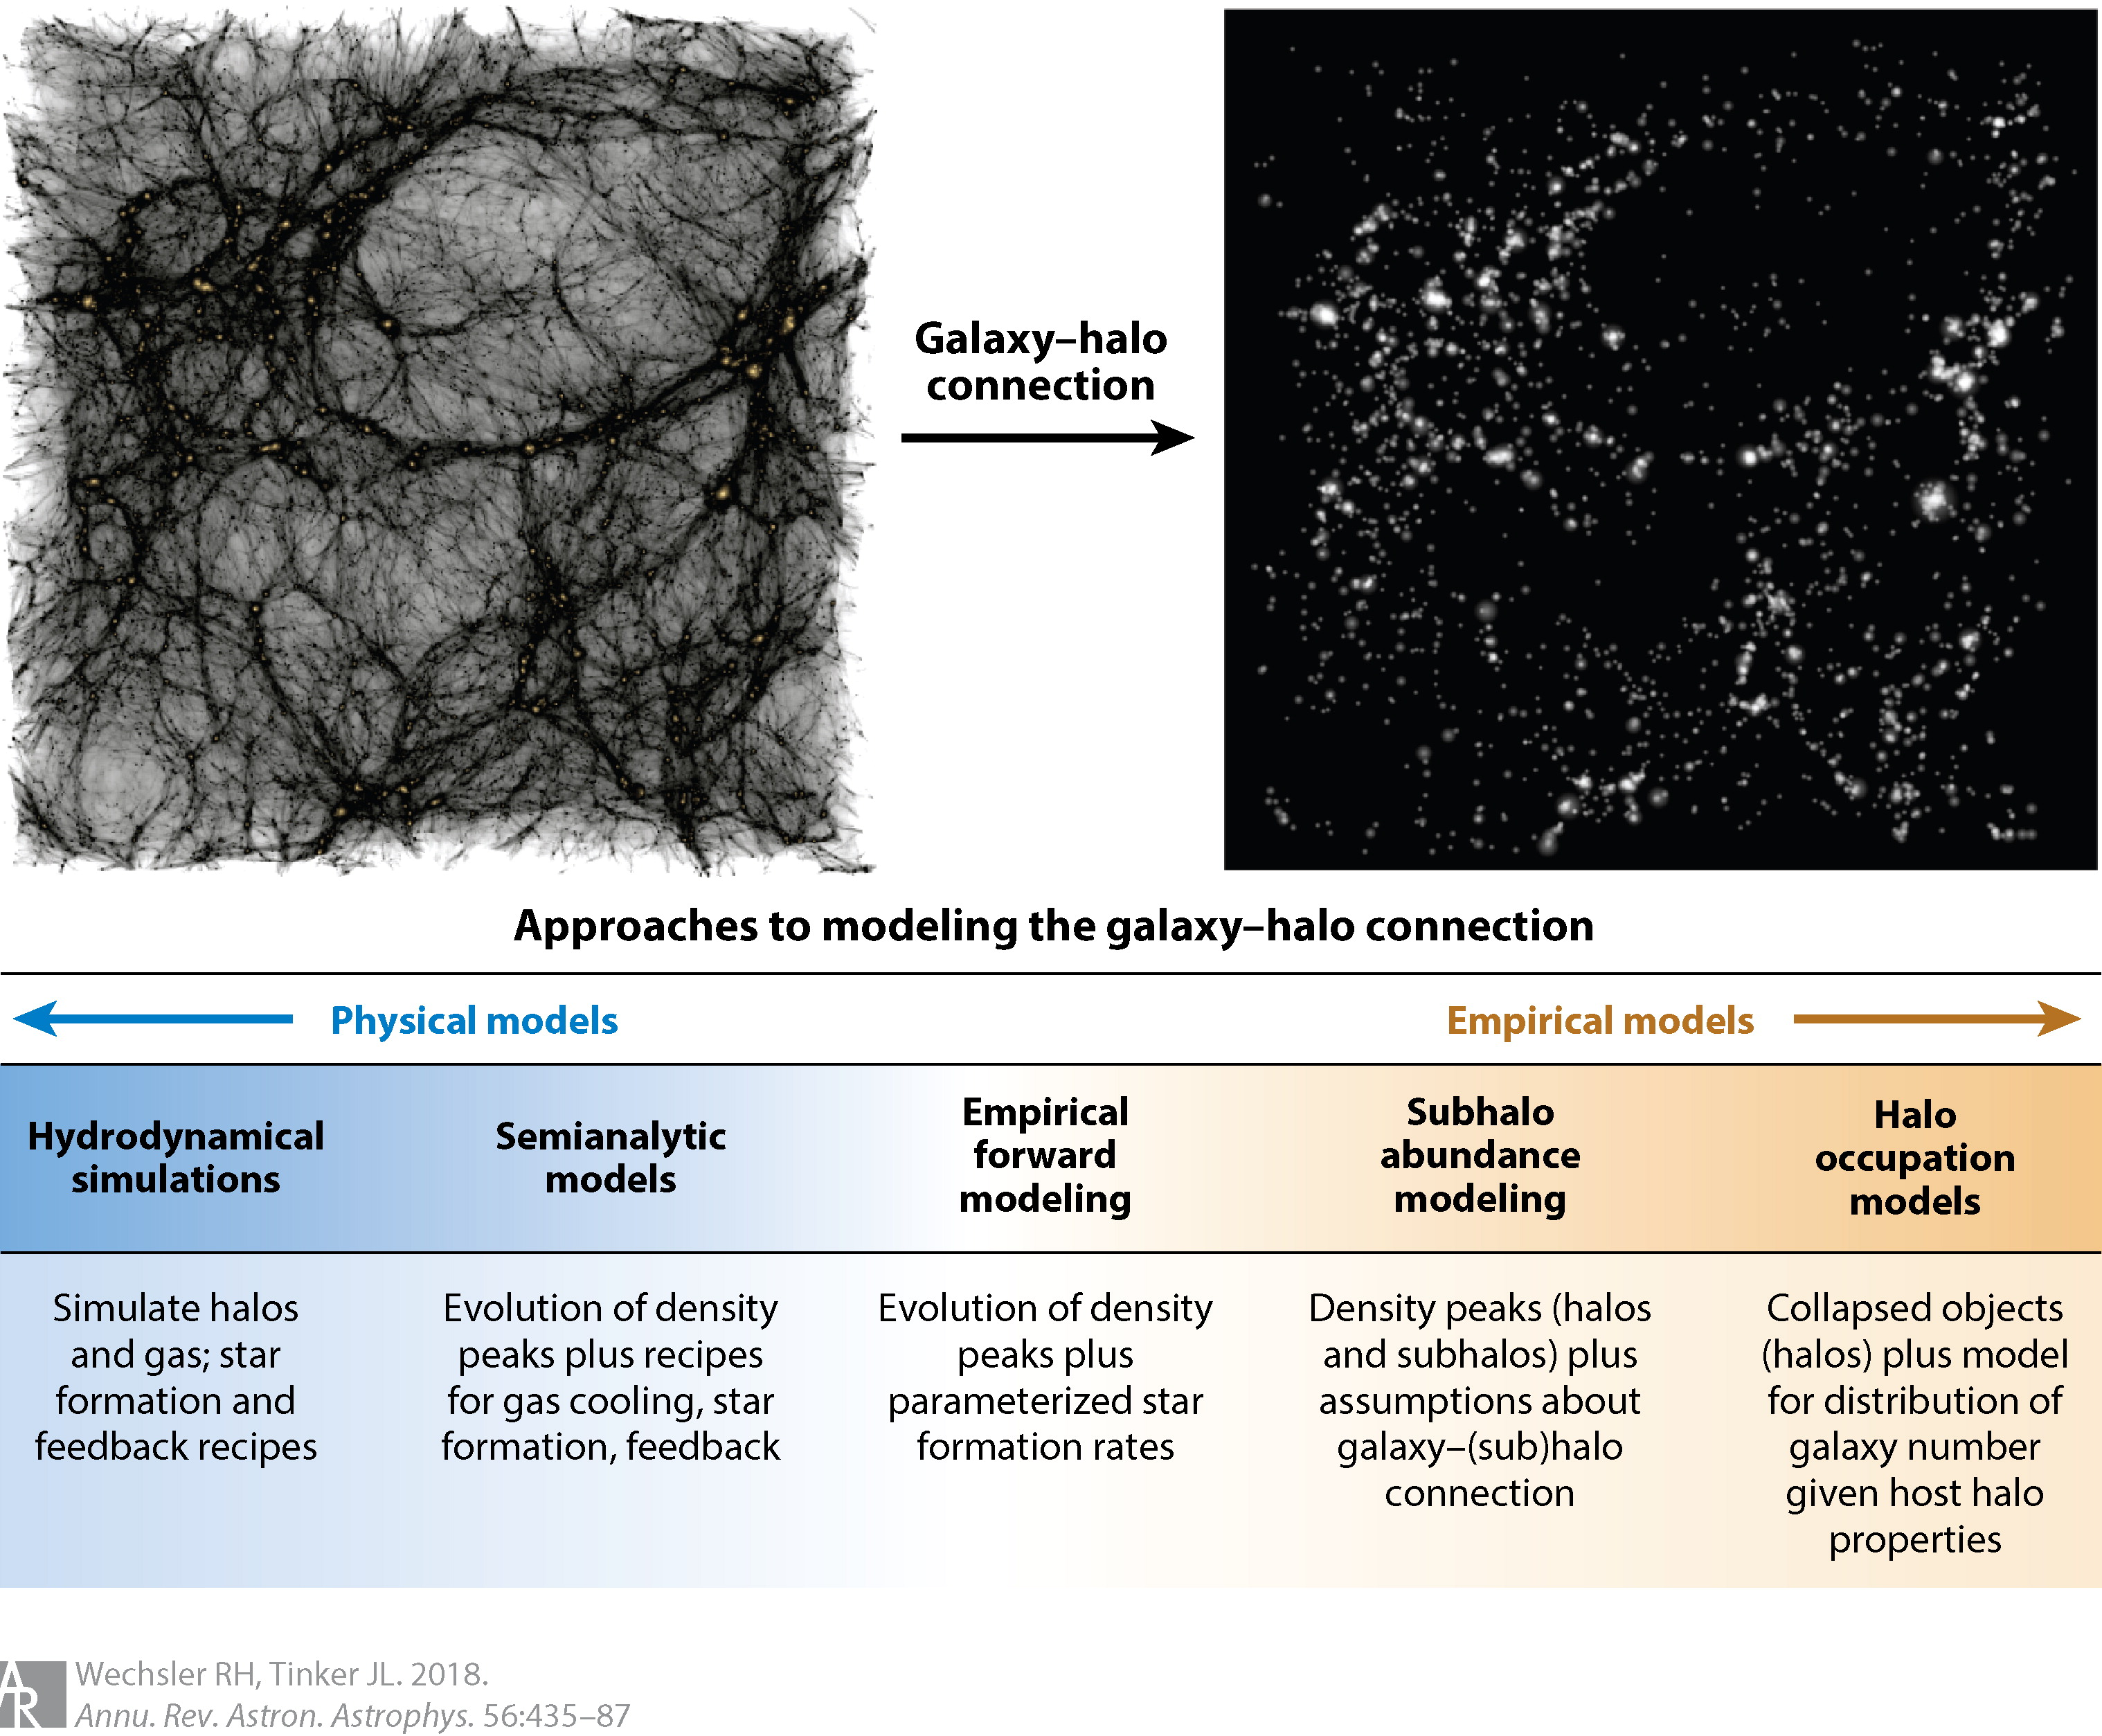
\includegraphics[width=0.8\textwidth]{galhalo.jpg}
    \caption{A visualization of the galaxy--halo connection and a range of modeling approaches. The top panel shows the dark matter distribution in a slice of a cosmological simulation, and the corresponding galaxy population modeled using abundance matching. The bottom panel outlines approaches ranging from physical models to empirical models for modeling the relationship between dark matter and galaxies. \emph{Figure 1 of \cite{wechsler_connection_2018}.}}
    \label{fig:galhalo}
\end{figure*}

This relationship is visualized in Figure~\ref{fig:galhalo}, showing the DM distribution of a cosmological simulation paired with its galaxy population using an empirically calibrated model.
The figure also outlines a range of models from the literature for describing this connection, from empirical to physical models.
Here I describe the models at each end of this range, as these are the ones utilized in this dissertation, but each model on this spectrum has important uses.

A description of the galaxy--halo connection that has proven broadly successful is \emph{halo occupation distribution} (HOD) modeling (e.g. \citealt{peacock_halo_2000,Seljak2000,BerlindWeinberg2002}). 
The HOD model posits the conditional distribution of the number of galaxies $N$ occupying a halo, typically conditioned on halo mass $M$: $P(N|M)$.
This model has only a handful of parameters while remaining flexible enough to fit observed galaxy samples well (e.g. \citealt{Zheng2005,reddick_connection_2013}).
However, this ``vanilla'' HOD is not sufficient.
Analyses have shown that the clustering of halos depends on halo properties beyond mass, including formation time and concentration, an effect is known as \emph{halo assembly bias} \citep{wechsler_concentrations_2002, Wechsler2006,mao_beyond_2018}.
This may propagate to the clustering of galaxies, dubbed \emph{galaxy assembly bias}, and must be taken into account in HOD modeling (e.g. \citealt{Tinker2008,hearin_introducing_2016}).
An HOD model with environment-dependent assembly bias is used in the cosmological inference approach presented in Chapter~\ref{chp:aemulus}.







\section{Redshift Surveys}

\begin{figure*}
    \centering
    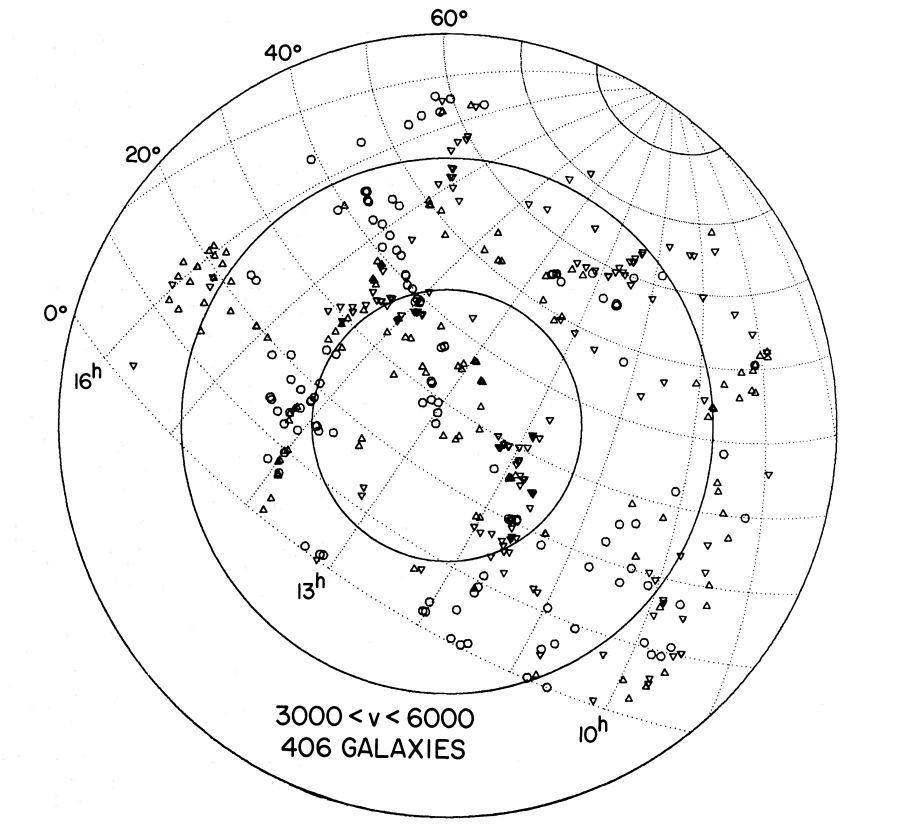
\includegraphics[width=0.6\textwidth]{cfa_survey}
    \caption{A sample of galaxies from the CfA redshift survey. Galaxies in the North Galactic Cap with $M<-18.5$ and velocity $3000<v<6000$ km s$\inv$ are shown in an equal-area sky projection. Filamentary structures, clusters, and voids can be seen visually. \emph{Figure 2b. of \cite{davis_survey_1982}.}}
    \label{fig:cfa_survey}
\end{figure*}

Over past several decades, we have built up immense 3-dimensional maps of the universe through observations of millions of galaxies.
These involve initial targeting using wide-field imaging, followed by spectroscopic observations to measure galaxy \emph{redshifts}.
The redshifts, measured by the shift of spectral lines from their rest-frame wavelength, indicate the velocity at which a galaxy is moving away from us and thus (assuming the velocity is dominated by the Hubble flow) its distance.
Early photographic observations of galaxies and  analyses of their angular distribution detected non-uniformity below a certain scale \citep{shapley_survey_1932,hubble_distribution_1934,seldner_new_1977,peebles_galaxy_2001}.
These results were extended to three dimensions by early redshift surveys, including \cite{gregory_comaa1367_1978} (238 galaxies around the Coma cluster), the KOS survey (\citealt{kirshner_million_1981}, 133 galaxies), and the CfA survey (\citealt{davis_survey_1982}, $\simo$2400 galaxies).
These confirmed the clustered distribution of galaxies, which can be identified visually even from these small samples. 
Figure~\ref{fig:cfa_survey} shows a sample of galaxies from the CfA survey, about which the authors write that the regions ``exhibit clustering in frothy, almost filamentary, patterns of connectedness surrounding empty holes on the sky.''

Modern redshift surveys have now observed orders of magnitude more galaxies and used their distributions to obtain some of the most stringent constraints on cosmological parameters.
The 2dF Galaxy Redshift survey \citep{Colless2001} observed $\simo$250,000, add the Sloan Digital Sky Survey (SDSS, \citealt{York2000}) observed nearly one million galaxy redshifts.
Galaxy power spectrum analyses of these surveys achieved measurements of the matter density ${\om}$ with a precision of $\simo$10\% \citep{cole_2df_2005, tegmark_cosmological_2006}.
Combining the results of baryon acoustic oscillations and redshift-space distortion analyses, SDSS has measured the parameter to $\sig$ to $\simo$3.5\%; a joint analysis with other cosmological measurements, including the cosmic microwave background, supernovae, and weak lensing, results in $\simo$1\% precision.

\begin{figure}
    \centering
    \includegraphics[width=0.6\textwidth]{desi_survey.jpg}
    \caption{A sample of galaxies from the DESI survey, around 40 years after the CfA survey of Figure~\ref{fig:desi_survey}. Around 400,000 galaxies are shown, out to $z \sim 0.9$ (3 $\hGpc$). DESI will observe nearly an order of magnitude more redshifts than this over the course of the survey. \emph{D. Schlegel/Berkeley Lab using data from DESI. Acknowledgment: M. Zamani (NSF's NOIRLab).}}
    \label{fig:desi_survey}
\end{figure}

Efforts are ongoing to map even more galaxies to increase the constraining power of large-scale structure.
The Dark Energy Spectroscopic Instrument (DESI, \citealt{Aghamousa2016}) has already cataloged nearly ten million redshifts and will observe multiple times that over the rest of the mission.
A slice through a sample of the galaxies DESI has already observed is shown in Figure~\ref{fig:desi_survey}; the filamentary structure hinted at in the CfA survey is now clear across the sky.
Future surveys are planned to measure yet more galaxy redshifts, including the Subaru Prime Focus Spectrograph \citep{takada_extragalactic_2014}, Euclid \citep{Laureijs2011}, and the Nancy Grace Roman Space Telescope \citep{Green2012}.

While galaxies are the dominant tracer observed for large-scale structure surveys given their multitude, other types of sources also provide valuable information.
Quasars, which are extremely luminous emission from active galactic nuclei{\emdash}accreting supermassive black holes{\emdash}at the centers of galaxies, are even more highly biased tracers of matter than galaxies, with $b \sim 2.5$ at $z \sim 1.5$ \citep{laurent_clustering_2017-3}.
Redshift surveys of quasars are the largest-volume maps of the universe we have, as we can observe quasars at immense distances thanks to their high luminosity.
Millions of quasars have been observed, with hundreds of thousands having spectroscopic redshifts, and more are being cataloged by current mission.
One such mission, \emph{Gaia}, and the opportunities it presents for large-scale structure science with quasars is discussed further in Chapter~\ref{chp:quaia}.



\section{Cosmological Inference}

The distribution of galaxies is extremely high-dimensional and complex, such that the actual positions of individual galaxies are impossible to model directly.
Luckily, these are largely irrelevant to the underlying cosmology that we care about; rather, the cosmological model makes strong predictions about the \emph{statistical} properties of the large-scale structure.
By computing the statistics of the galaxy distribution, we can compare our observations to models and infer the cosmological model parameters, as well as learn where our models are insufficient to describe the data.

Standard cosmological inference from galaxy clustering relies on low-order statistics of the galaxy distribution. 
The most important statistic is the \emph{two-point correlation function} (\cf), denoted $\xi(r)$, which is defined as the excess probability $\delta P$ of finding a galaxy in a volume element $\delta V$ a given separation $r$ apart from another galaxy compared to a random distribution:
\begin{equation}
    \delta P = n[1+\xi(r)]\delta V ~,
\end{equation}
where $n$ is the mean galaxy number density.
Below scales of $r \sim 10 \hMpc$, the \cf roughly follows a power law, $\xi(r) \sim (r/r_0)^{-\gamma}$, where $r_0$ is a characteristic scale (found to be $r_0 \sim 5 \hMpc$) and $\gamma$ is the power law index, measured to be $\gamma \sim 1.8$.
The \cf can be estimated from galaxy samples with estimators that take into account the finite, irregular window function of the survey, using estimators such as that proposed by \cite{DavisPeebles1983} or \cite{LandySzalay1993}; these are discussed in much more detail in Chapter~\ref{chp:cfe}.

We can compare the measured \cf to a model prediction to find the model parameters that most closely describe the data.




\section{Chapter Notes}

In this thesis, I present new tools for studying large-scale structure and galaxy formation from multiple angles.
These tools range from statistical and machine learning methods to simulation-based approaches and observational data catalogs.

In Chapter~\ref{chp:aemulus}, I present an approach for cosmological inference using probabilistic machine learning and N-body simulations, and demonstrate the importance of environment-dependent clustering statistics.
In Chapter~\ref{chp:cfe}, I develop a new statistic for galaxy clustering that obviates issues of traditional, binned clustering statistics.
I explore a new approach to characterizing the dark matter distribution in cosmological simulations using symmetry-preserving quantities in Chapter~\ref{chp:eqcosmo}, relevant to understanding the galaxy--halo connection.
Chapter~\ref{chp:quaia} presents the largest-volume spectroscopic quasar catalog ever constructed, based on \emph{Gaia} and unWISE, which is an unprecedented sample for large-scale structure analyses.
Finally, in Chapter~\ref{chp:anomalies} I look at using deep learning to identify anomalous galaxy images with the goal of widening the discovery possibilities of galaxy surveys.

Chapters~\ref{chp:cfe} and \ref{chp:anomalies} have been refereed and published in the astronomical literature (\emph{The Astrophysical Journal} and \emph{Monthly Notices of the Royal Astronomical Society}, respectively).
Chapter~\ref{chp:aemulus} has been submitted to \emph{The Astrophysical Journal} and is under review.
Chapters~\ref{chp:eqcosmo} and \ref{chp:quaia} are in the final draft stage and will be submitted to journals soon.
The code associated with all of these chapters is publicly available online.\footnote{\url{https://github.com/kstoreyf}}

While the analyses in each Chapter were conducted in collaboration with my co-authors and the support of many others, the majority of the work and the (near-)entirety of the writing in this dissertation is mine. 
I describe the contributions of myself and my coauthors to each Chapter here:
\begin{enumerate}[leftmargin=4\parindent]
    \item[Chapter~\ref{chp:aemulus}:] I developed the idea for this project with Jeremy Tinker and the rest of the \aemulus collaboration. I led the development of this project in conjunction with Jeremy Tinker, with input from Zhongxu Zhai, Joseph DeRose, Risa H. Wechsler, and Arka Banerjee. I implemented all of the code, which used Zhongxu Zhai's code as a starting point and simulations led by Joseph DeRose. I wrote the paper text and received feedback from the rest of the collaboration.
    \item[Chapter~\ref{chp:cfe}:] I developed the idea for this project with David W. Hogg. I implemented the code and worked out the mathematical proof. I wrote the paper with input from David W. Hogg.
    \item[Chapter~\ref{chp:eqcosmo}:] I conceived the idea for this project, and developed it in collaboration with David W. Hogg, Shy Genel, and Soledad Villar. I implemented it with additional feedback from Soichiro Hattori, Austen Gabrielpillai, and Yongseok Jo. I wrote the chapter text, with feedback from these collaborators.
    \item[Chapter~\ref{chp:quaia}:] I developed the idea for this project in collaboration with David W. Hogg and Hans-Walter Rix. I implemented it with additional feedback from Anna-Christina Eilers and Giulio Fabbian. I wrote the text of the chapter with input from these collaborators.
    \item[Chapter~\ref{chp:anomalies}:] The idea for this project was conceived at the Kavli Summer Program in Astrophysics in 2019, in collaboration with Marc Huertas-Company and Alexie Leauthaud. I led project development and implementation, with feedback from Nesar Ramachandra, Francois Lanusse, and J. Xavier Prochaska. Yifei Luo took observations and reduced the data, Song Huang contributed data support, and J. Xavier Prochaska contributed analysis support. I wrote the text of the paper with input from these collaborators.
\end{enumerate}




\chapter{Two-point statistics without bins: A continuous-function generalization of the correlation function estimator for large-scale structure}
\setcounter{section}{-1}
\label{chp-cfe}
%This chapter is published in \emph{the Astrophysical Journal} with title ``Two-point statistics without bins: A continuous-function generalization of the correlation function estimator for large-scale structure'' and full author list Kate Storey-Fisher and David W. Hogg \citep{storey-fisher_two-point_2021}.


% This project is part of the Continuous-Function Estimator project
% Copyright 2021 the authors.

%\documentclass[modern]{aastex62}

% \usepackage[sort&compress]{natbib}
% \usepackage{graphicx}
% \usepackage{xspace}
% \usepackage{xcolor}
% \usepackage{bm}
% \usepackage{mathtools}
% \parindent=19pt

% aastex parameters
%\received{XXX}
%\revised{not yet}
%\accepted{YYY}
%\submitjournal{ApJ}
% \shorttitle{a continuous correlation function estimator}
% \shortauthors{storey-fisher and hogg}

\graphicspath{{figures/figures_cfe/}}



% affiliations
% \newcommand{\ccpp}{\affiliation{%
%     Center for Cosmology and Particle Physics,
%     Department of Physics,
%     New York University}}
% \newcommand{\flatiron}{\affiliation{%
%     Flatiron Institute, Simons Foundation}}
% \newcommand{\cds}{\affiliation{%
%     Center for Data Science,
%     New York University}}
% \newcommand{\mpia}{\affiliation{%
%     Max-Planck-Institut f\"{u}r Astronomie, Heidelberg}}


%\begin{document}%\sloppy\sloppypar\raggedbottom\frenchspacing

% \title{\textbf{Two-point statistics without bins: A continuous-function generalization of the correlation function estimator for large-scale structure}}

% \author[0000-0001-8764-7103]{Kate Storey-Fisher}
% %\email{k.sf@nyu.edu}
% \ccpp
% \correspondingauthor{Kate Storey-Fisher \texttt{<\href{mailto:k.sf@nyu.edu}{k.sf@nyu.edu}>}}

% \author[0000-0003-2866-9403]{David W. Hogg}
% \ccpp
% \cds
% \mpia
% \flatiron

%\begin{abstract}\noindent
\section{Chapter Abstract}

The two-point correlation function (2pcf) is the key statistic in structure formation; it measures the clustering of galaxies or other density field tracers. Estimators of the 2pcf, including the standard Landy--Szalay (LS) estimator, evaluate the 2pcf in hard-edged separation bins, which is scientifically inappropriate and results in a poor trade-off between bias and variance. We present a new 2pcf estimator, the Continuous-Function Estimator, which generalizes LS to a continuous representation and obviates binning in separation or any other pair property. Our estimator, inspired by the mathematics of least-squares fitting, replaces binned pair counts with projections onto basis functions; it outputs the best linear combination of basis functions to describe the 2pcf. The choice of basis can take into account the expected form of the 2pcf, as well as its dependence on pair properties other than separation. We show that the Continuous-Function Estimator with a cubic-spline basis better represents the shape of the 2pcf compared to LS. We also estimate directly the baryon acoustic scale, using a small number of physically-motivated basis functions. Critically, this leads to a reduction in the number of mock catalogs required for covariance estimation, which is currently the limiting step in many 2pcf analyses. We discuss further applications of the Continuous-Function Estimator, including determination of the dependence of clustering on galaxy properties and searches for potential inhomogeneities or anisotropies in large-scale structure.
%\end{abstract}


\section{Introduction}

The large-scale structure (LSS) of the Universe is critical to our understanding of fundamental cosmology. 
It encodes information about the physics of the early Universe and the subsequent expansion history \citep{SunyaevZeldovich1970, HuSugiyama1996, Riess1998}.
In particular, LSS measures the Baryon Acoustic Oscillation (BAO) scale \citep{Cole2005, Eisenstein2005}, which results from density fluctuations in the baryon--photon fluid.
The distance traveled by these density waves before recombination imprints a feature on the statistical description of the LSS, which can be used to determine the characteristic BAO length scale \citep{PeeblesYu1970, EisensteinHu1998}.
The LSS also contains the signature of redshift-space distortions caused by the peculiar velocities of galaxies, which are used to measure the growth rate of structure \citep{Kaiser1987}.
Additionally, the LSS can be used to constrain galaxy formation in conjunction with models of galaxy bias (e.g., \citealt{Hamilton1988},  \citealt{Li2006}, \citealt{Zehavi2011}, \citealt{Durkalec2018}).
With current observations, the LSS is well-described by a cold dark matter model with a cosmological constant, the standard $\Lambda$CDM model (e.g., \citealt{Alam2017}).
Upcoming galaxy surveys including DESI \citep{Aghamousa2016}, Euclid \citep{Laureijs2011}, and LSST \citep{Ivezic2018} will observe larger volumes with improved measurements, allowing us to test $\Lambda$CDM to even higher precision.

The most important statistic for characterizing the LSS is the two-point correlation function (\cf).
\new{It measures the excess probability of finding two galaxies are separated by a given distance, compared to a spatially random Poisson distribution;} effectively, it characterizes the strength of clustering at a given spatial scale.
The \cf is the primary tool for extracting cosmological information from galaxy redshift surveys.
Such correlation function analyses include \cite{Hawkins2003} for the 2dF Galaxy Redshift Survey (2dFGRS, \citealt{Colless2001}), \cite{Alam2017} for the Baryon Oscillation Spectroscopic Survey (BOSS, \citealt{Dawson2013}) DR12 analysis, and \cite{Elvin-Poole2017} for the Dark Energy Survey (DES, \citealt{DES2005}).

Traditionally, the \cf is estimated in bins of radial separation.
\new{Recent work has focused on the inappropriateness and limitations of binning in astrophysical contexts.}
Broadly, binning adds arbitrary boundaries between continuous data; results should not depend on bin choice, yet they sometimes do.
\new{It results in the well-known trade-off between bias and variance: fewer bins may bias the result (i.e. reduce the accuracy), while more bins will increase the variance of measurement (i.e. reduce the precision)}.
Finite-width bins also result in a loss of information about the property in which one is binning.
\new{These issues have been demonstrated in various fields of astrophysics.}
\new{\cite{Kipping2010} showed that temporal binning of transit lightcurves results in inaccurately recovered system parameters.}
\cite{Lanzuisi2017} noted that the choice of binning axis impacts the detected correlation between the luminosity of active galactic nuclei and their host galaxies; \cite{Grimmett2020} devised a method to investigate this correlation in a continuous manner using a hierarchical Bayesian model, eliminating the need for binning.
\new{\cite{Brout2020} found that binning supernovae data causes a larger systematic error in inferred cosmological parameters, while performing an unbinned analysis allows the data to self-calibrate out these systematic uncertainties.}
From this literature it is clear that, when analyzing smooth quantities, binning is sinning.

\new{The issue of binning is particularly relevant in LSS analyses.}
\cite{Bailoni2016} explored the dependence of clustering analyses on the number of redshift bins, finding a non-negligible difference in cosmological parameter uncertainties.
\new{\cite{Schneider2009} showed that in cosmic shear analyses, increasing the number of bins increases the probability that the correlation function is not positive semi-definite, and therefore not statistically valid.}
The implications for BAO analyses were explored by \cite{Percival2014}, who found that the effects of bin width are small but non-negligible; they showed that there is an optimal bin width given the analysis method that trades off statistical uncertainty against bias in the derived BAO peak location.
Generally, the loss of information inherent in binning may become a critical bottleneck as we work towards extreme precision in LSS analyses.

Another critical issue for \cf analyses is that the error on the inverse covariance matrix estimate depends on the number of bins.
A larger number of bins results in a larger error that propagates to the estimated parameters \citep{Dodelson2013}.
This can be balanced by using a large number of mock galaxy catalogs, but these can be exceedingly expensive to generate.
Covariance matrix estimation is currently the limiting step in many LSS analyses.
For galaxy clustering, on the order of 1000 mock catalogs tailored to the survey needed to achieve the desired precision on the parameters \citep{Percival2014}.
\new{Weak lensing analyses especially suffer from this issue given their very high-dimensional data vectors (for a review see \citealt{Mandelbaum2018a}).}
As survey size increases and we work towards higher precision, the requirements on the covariance matrix will get even more stringent; the connection of this limiting step with bin choice merits scrutiny of binning in \cf analyses.

Estimators of the \cf have been studied extensively (e.g., \citealt{PeeblesHauser1974}; \citealt{DavisPeebles1983}; \citealt{Hamilton1993}).
One of the difficulties in performing a two-point estimate is that nontrivial survey boundaries would bias a direct summation of pair counts.
To account for the boundaries as well as \new{corrupted regions (e.g. by bright foreground stars)}, typically a large set of random points are \new{Poisson-distributed} within the acceptable survey window.
The pairwise correlations of these unclustered points are used to normalize out the survey window.
The current standard estimator, proposed by \cite{LandySzalay1993} (hereafter \LS), takes this approach.
It involves a summation of the data--data pairs $DD$ in each separation bin, \new{and uses the random--random pairs $RR$ to perform this edge-correcton;} the data--random pairs $DR$ are incorporated to improve the bias and variance properties of the estimator \new{(see e.g. \citealt{Hamilton1993})}.
The \LS estimator of the correlation function $\hat{\xi}_k$ for the $k^\mathrm{th}$ bin in separation $r$ is defined as
\begin{equation} \label{eq:lsintro}
\hat{\xi}_k = \frac{DD_k - 2DR_k + RR_k}{RR_k}
\end{equation}
\new{where we have assumed the binned pair counts are normalized by the total number of pairs for each set of catalogs}.
Compared with other estimators based on simple combinations of $DD$, $DR$ and $RR$, \LS has been shown to have the lowest bias and variance \citep{Kerscher2000}.
Estimators of the \cf must also take into account the imperfect nature of the survey, including systematic effects, the target completeness, and fiber collisions.
To account for these, each galaxy pair is typically assigned a weight, and pair counts are replaced by the sum of pair weights.

Variations on traditional \cf estimation have been proposed in recent years.
\cite{Demina2016} replaced the $DR$ and $RR$ terms with an integral over the probability map, reducing computation time and increasing precision.
An estimator proposed by \cite{VargasMagana2013} iterates over sets of mock catalogs to find an optimal linear combination of data and random pair counts, reducing the bias and variance.
An alternative estimator, the marked correlation function (e.g., \citealt{WhitePadmanabhan2009}), avoids the use of a random catalog altogether: it considers the ratio between the \cf and a weighted correlation function in which weights are assigned based on galaxy properties, such as the local density.
These estimators have all taken probabilistic approaches; others have taken a likelihood approach.
\cite{BaxterRozo2013} introduced a maximum likelihood estimator for the \cf, which achieves lower variance compared to the \LS estimator, enabling finer binning and requiring a smaller random catalog for the same precision.

These estimators present improvements to \LS, but they are still limited to estimates in separation bins.
Some require additional computational costs or layers of complexity, so the standard formulation of \LS continues to be the default estimator used in most analyses.

In this \documentname, we present a new estimator for the correlation function, \est, which generalizes the \LS estimator to produce a continuous estimation of the \cf. 
\Est projects the galaxy pairs onto a set of continuous basis functions and directly computes the best-fit linear combination of these functions.
The basis representation can depend on the pair separation as well as other desired properties, and can utilize the known form of the \cf.
For tophat basis functions, the estimator exactly reduces to the \LS estimator. 
\Est removes the need for binning and produces a more representative estimate of the \cf with fewer basis functions, \new{increasing the accuracy and} reducing requirements on mock catalogs for covariance matrix computation.
It is particularly well-suited to the analysis of LSS features such as the BAO peak; we find that we can accurately locate the peak with fewer components compared to standard analyses.

This \documentname is organized as follows. 
In Section~\ref{sec:motiv}, we motivate our estimator and explain its formulation, \new{and derive the connection to least-squares fitting}.
We demonstrate its application on a simulated dataset, including a toy BAO analysis, in Section~\ref{sec:experiments}.
In Section~\ref{sec:discuss}, we discuss the implications, limitations, and other possible extensions and applications of the estimator. 
\new{We summarize in Section~\ref{sec:summary_cfe}.}

\section{Motivation and Formulation} 
\label{sec:motiv}

In this \documentname, we use the following notation.
We write vectors in bold and lowercase, e.g. $\vv{}$; tensors in bold and uppercase, e.g. $\TT{}$; and unstructured data blobs in sans serif, e.g. $\GG{}$.
A hat above a symbol, e.g. $\bld{\hat{\xi}}$, indicates an estimate of the value.

\subsection{Standard Two-Point Correlation Function Estimation}
\label{sec:ls}

The standard approach to estimating the two-point correlation function involves counting pairs of tracers within a survey volume as a function of separation scale.
Let's assume we have a data catalog with $N_D$ objects within a sky volume.
We also require a random catalog with $N_R$ objects Poisson-distributed throughout the same volume.
We can define a set of separation bins which we will use to estimate the \cf at various scales.
We are then ready to sum in each bin the relevant pairs of objects within and across our catalogs.
In standard notation, these pair counts are written as $DD$, $DR$, and $RR$, as in \eqt{eq:lsintro}.
To clarify that these are in fact vectors, with length $K$ where $K$ is the number of bins, we use the symbol $\vv{}$; then, for example, the data--data pair counts $DD$ become $\vv{DD}$.
We can then write the \LS estimator as 
\begin{equation} \label{eq:ls}
    \bld{\hat{\xi}} = \frac{\vv{DD} - 2\,\vv{DR} + \vv{RR}}{\vv{RR}} ~.
\end{equation}
\new{We also make explicit the pair-count normalization factors, defining $\NN{DD} \equiv \frac{2}{\NN{D}\,(\NN{D}-1)}$, $\NN{DR} \equiv \frac{1}{\NN{D}\,\NN{R}}$, and $\NN{RR} \equiv \frac{2}{\NN{R}\,(\NN{R}-1)}$.}
The components of the pair-count vectors can then be written as
\begin{eqnarray}\displaystyle
    \label{eq:ls1}
    % \adjustlimits aligns the subscripts with and without primes, which are diff heights
    \left[ \vv{DD} \right]_k &\equiv& \frac{1}{\NN{DD}} \adjustlimits \sum_{n} \sum_{n' < n} i(g_k < |\bld{r}_n - \bld{r}_{n'}| < h_k) \\ 
    \left[ \vv{DR} \right]_k &\equiv& \frac{1}{\NN{DR}}\sum_{n} \sum_{m} i(g_k < |\bld{r}_n - \bld{r}_m| < h_k) \\
    \label{eq:ls3}
    \left[ \vv{RR} \right]_k &\equiv& \frac{1}{\NN{RR}} \adjustlimits\sum_{m} \sum_{m'<m} i(g_k < |\bld{r}_m - \bld{r}_{m'}| < h_k) ~,
\end{eqnarray}
where $\left[ \vv{} \right]_k$ is the pair counts in bin $k$ (which has bin edges $g_k$ and $h_k$), $i$ is an indicator function that returns $1$ if the the condition is true and otherwise returns $0$, $\bld{r}$ is the tracer position, the $n$ and $n'$ indices index data positions, and the $m$ and $m'$ indices index random catalog positions.
The sums are over unique pairs, and for auto-correlations they exclude self-pairs; the normalization prefactors then account for the total number of possible pairs, explaining the difference between the auto- and cross-correlation factors.
The tracer position can be in real or redshift space, or broken down into the transverse and line-of-sight directions in the anisotropic correlation function; in this \documentname we consider the isotropic real-space \cf for simplicity, but the estimators detailed here apply equally well to these alternative configurations.
The estimator is also easily applicable to cross-correlations of two datasets.
 
The \LS estimator is known to be optimal (i.e. it is unbiased and has minimum variance) under a particular set of conditions: in the limit of unclustered data, for a data volume much larger than the scales of interest, and an infinitely large random catalog. 
In practice the latter two limits are sufficiently satisfied, but the data we are interested in are clustered.
\cite{VargasMagana2013} show that for clustered data, the \LS estimator has lower variance than other estimators, but does not reach the Poisson noise limit.
When applied to clustered data, \LS does show a bias on very large scales ($>$130 \hmpc), but the bias is significantly smaller than that of most other estimators (\citealt{Kerscher1999}, \citealt{VargasMagana2013}).
\LS is also less sensitive to the number of random points than other estimators \citep{Kerscher2000}.
While \LS has been sufficient for past analyses, its persisting bias and suboptimal variance under imperfect conditions mean that improvement is possible, and will be necessary for realistic large-scale structure measurements on modern datasets.


\subsection{\Est}
\label{sec:est}

\new{We present an estimator, \est, that generalizes the \LS estimator in a manner inspired by least-squares fitting.
We first provide an intuitive description of the estimator, followed by the mathematical formulation; we then derive the connection to least-squares in Section~\ref{sec:leastsq}.}

\new{\Est replaces the binned pair counts of \LS with a \textit{projection} of the pairs onto any set of basis functions; the linear superposition of these projections is our estimate of the \cf.
Essentially, \est outputs the best-fit linear combination of basis functions to describe the \cf.
This is most straightforward to see for the case of tophat (rectangular) basis functions.
Each pair is projected onto the tophat functions, with one of the functions getting a contribution of 1 and the rest getting 0; the sum of these contributions for all pairs produces the total data projection onto each tophat.
Note that this is equivalent to slotting the pairs into separation bins and summing them to get the binned pair counts, as in standard binned estimators.
We can now replace the tophat functions with any set of basis functions; when we project the pairs onto these functions, the functions may get fractional contributions as they no longer have to be bin-like.
(For simplicity we consider basis functions that are only depend on pair separation, but in fact \est can perform projections onto bases that are functions of any pair properties.)
The sum of these contributions will give the total data projection onto the set of basis functions.}

\new{We perform the same procedure with all pairs in the random catalog in order to obtain the random-random projection, and similarly with the data-random projection.
In general, the continuous functions will not be orthogonal or normalized, so we also require a normalization matrix.
This is constructed from the outer product of the random-random pair projections, for technical reasons described below.
We can then combine these projections in a manner similar to the pair-count combination of the \LS estimator, with the denominator replaced by the normalization matrix; this produces a final set of \textit{amplitudes} for the basis functions. 
The \cf estimate is simply the sum of the basis functions weighted by these amplitudes.
It can be evaluated at any pair separation, as the basis functions are continuous, producing a continuous correlation function. 
This process is shown schematically in Figure~\ref{fig:schematic}, with a choice of cubic spline basis functions (for more details on the spline see Section~\ref{sec:spline}).}

\begin{figure}[t!]
    \centering
    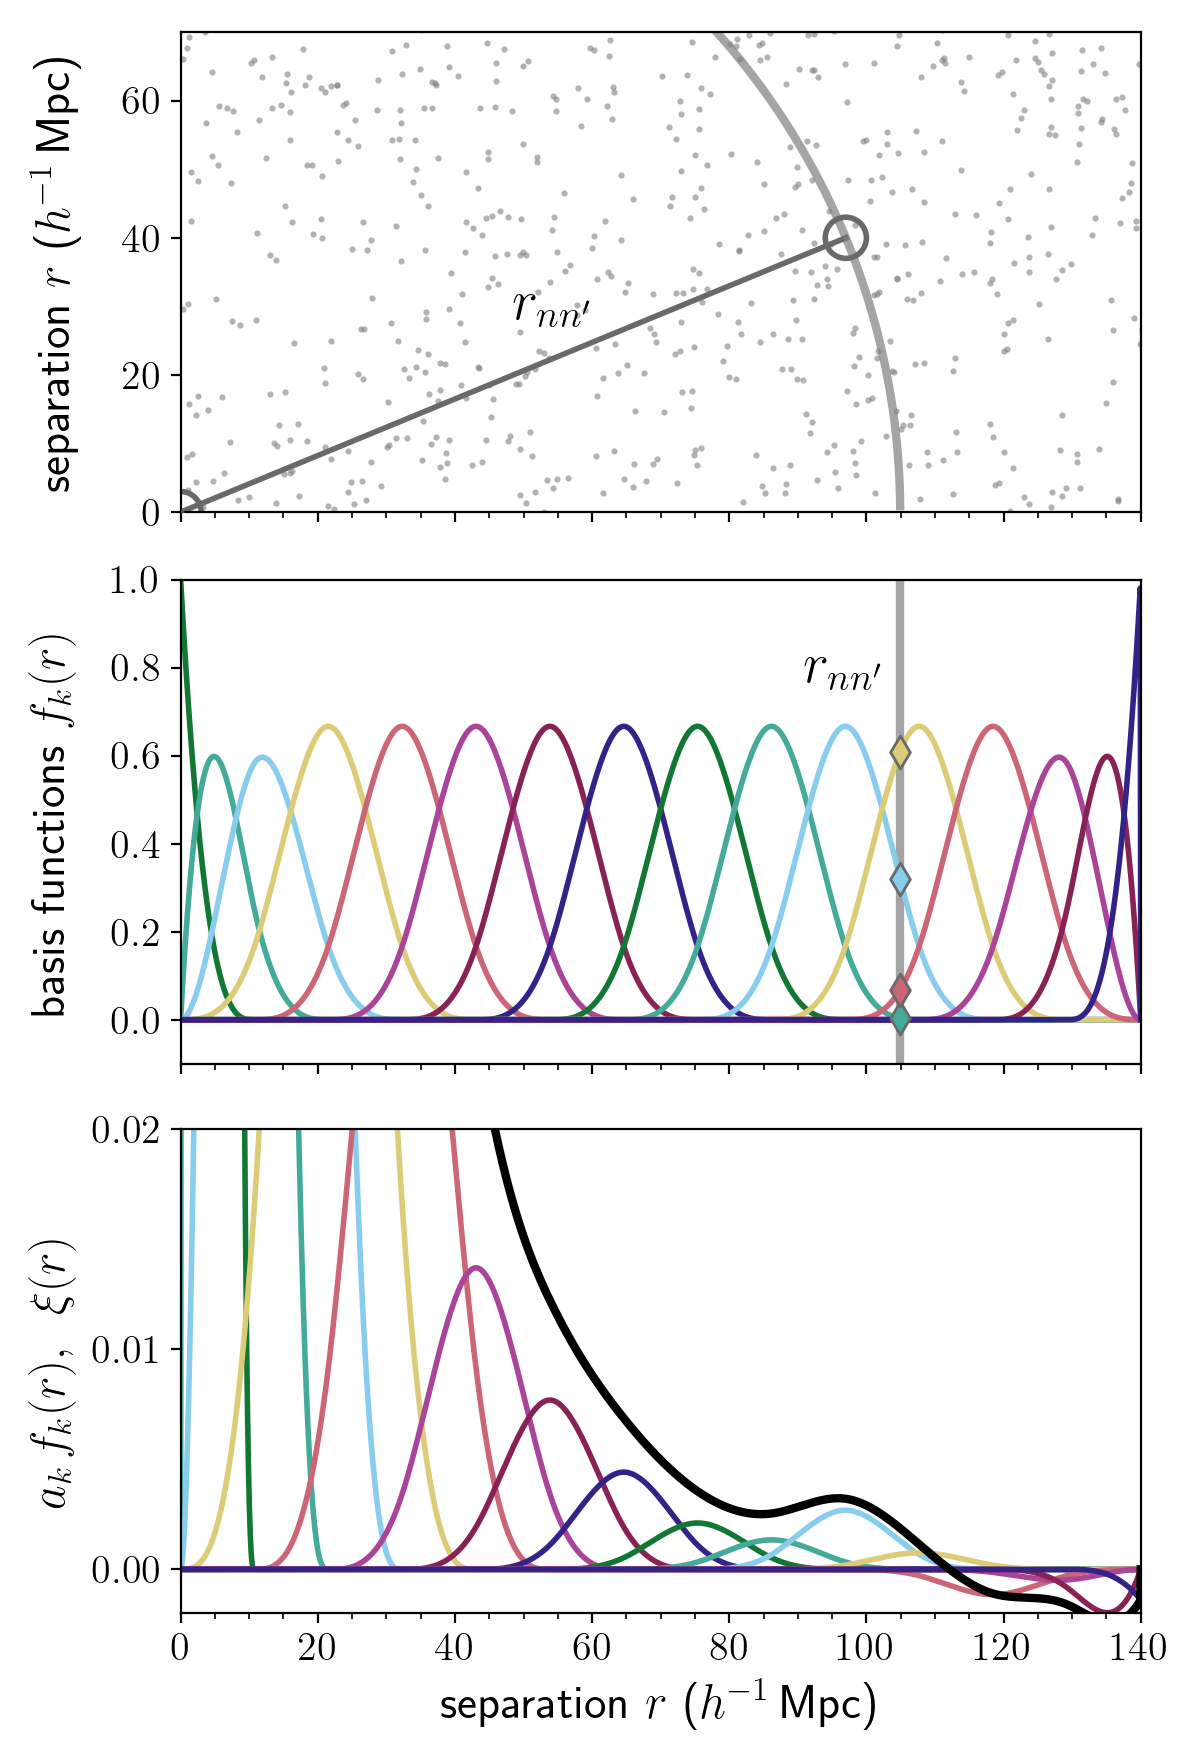
\includegraphics[width=0.6\textwidth]{schematic_spline}
    \caption{\new{A schematic illustrating how \est works. The top panel shows a slice of a dataset; each point represents a galaxy. One pair $\GG{n n'}$ is highlighted, with separation $r_{n n'}$ (grey line). The middle panel shows how \est performs the projection of the pair onto a chosen basis. Here we use cubic spline basis functions $f_k$ (see Section~\ref{sec:spline}; colored lines). The contribution of the pair to each basis function is given by the value of the function at separation $r_{n n'}$ (grey line); this quantity is $f_k(r_{n n'})$ (colored diamonds). The bottom panel shows the basis functions weighted by the final amplitudes $a_k$, given by the combination of contributions by all pairs. The final \cf estimate $\xi(r)$ (thick black line) is the sum of these, as given by \eqt{eq:xi_proj}.}}
    \label{fig:schematic}
\end{figure}

\new{We formalize this concept by generalizing the \LS estimator detailed in Section~\ref{sec:ls}.}
We take the indicator function $i$ to be any set of basis functions $\ff$, which returns a vector of length $K$, the number of bases.
We further generalize the arguments of the function to any properties of the galaxy pair, rather than just the separation between pairs; we call $\GG{ij}$ the data payload for the pair of galaxies $i$ and $j$.
This gives us, instead of pair counts, a vector $\vv{}$ of projections of the pairs onto basis functions, defined as
\begin{eqnarray}\displaystyle
    \label{eq:vdd}
    \vv{DD} &\equiv& \frac{1}{\NN{DD}} \adjustlimits \sum_{n} \sum_{n'<n} \ff(\GG{n n'}) \\
    \label{eq:vdr}
    \vv{DR} &\equiv& \frac{1}{\NN{DR}} \sum_{n} \sum_{m} \ff(\GG{n m}) \\
    \label{eq:vrr}
    \vv{RR} &\equiv& \frac{1}{\NN{RR}} \adjustlimits \sum_{m} \sum_{m'<m} \ff(\GG{m m'}) ~.
\end{eqnarray}
\new{We also require a normalization matrix to ensure that the estimator remains affine-invariant in the case of non-orthogonal basis functions.}
We thus define a projection tensor $\TT{RR}$ based on the autocorrelation of the random catalog, 
\begin{equation}
    \label{eq:Trr}
    \TT{RR} \equiv \frac{1}{\NN{RR}} \adjustlimits \sum_{m} \sum_{m'<m} \ff(\GG{m m'}) \cdot \ff\T(\GG{m m'}) ~,
\end{equation}
\new{where the exact formulation is motivated in Section~\ref{sec:leastsq} and satisfies the required affine invariance of the estimator as shown in Appendix~\ref{sec:affine}.}

We can now define \est as
\begin{equation}
    \label{eq:xi_proj}
    \hat{\xi}(\GG{\ell \ell'}) \equiv \bld{\hat a}\T \cdot \ff(\GG{\ell \ell'}) ~,
\end{equation}
where $\GG{\ell \ell'}$ contains the data values at which to evaluate $\bld{\hat{\xi}}$, and $\bld{\hat a}$ is a $K$-vector of the computed amplitudes of the basis functions
\begin{equation}
    \label{eq:amplitude}
    \bld{\hat a} \equiv \TT{RR}\inv \cdot (\vv{DD} - 2\,\vv{DR} + \vv{RR}) ~.
\end{equation}
\new{This parallels the pair-count combination of the \LS estimator, generalized to a least-squares fitting formulation.
As we will see in the next section,} the linear combination of vectors projects the pair information onto the features encoded by the basis functions, and the projection tensor performs a rescaling of these features.

We emphasize that $\GG{\ell \ell'}$ in \eqt{eq:xi_proj} does not represent a real pair of galaxies, but instead allows us to evaluate the \cf at any set of separations or other properties.
We can think of it as the data for an imaginary pair of galaxies $\ell$ and $\ell'$ that have a separation $r$ at which we want to evaluate $\bld{\hat{\xi}}$, and we would compute $\bld{\hat{\xi}}$ for such a pair at every separation in which we are interested.
As the formulation of \est is extremely general, we could choose basis functions that depend on other galaxy properties (see Section~\ref{sec:applications_cfe}); then, we would also choose each $\GG{\ell \ell'}$ pair to have values of these properties at which we want to evaluate $\bld{\hat{\xi}}$.
In the experiments in this \documentname, however, we will only take into account the separation between pairs, so we will write $\hat{\xi}(r)$.

\Est reduces to the \LS estimator when we choose $\ff$ to be a set of tophat functions in pair separation.
Explicitly, from our galaxy pair data $\GG{n n'}$, we use only their separation,  $|\bld{r}_n - \bld{r}_{n'}|$.
We can then define a set of $K$ basis functions $\ff$ as
\begin{equation}
    \label{eq:ff_separation}
    f_k(\GG{n n'}) =  i(g_k < |\bld{r}_n - \bld{r}_{n'}| < h_k) ~,
\end{equation}
where $k$ denotes the tophat component with edges $g_k$ and $h_k$ as before.
In this case the $\vv{DD}$, $\vv{DR}$ and $\vv{RR}$ projection vectors become binned pair counts.
The $\TT{RR}$ tensor becomes diagonal as the bins are orthogonal, with its diagonal elements equal to the elements of the $\vv{RR}$ vector.
\new{Then the amplitudes $\bld{\hat a}$ are exactly the \cf estimate given by \LS, and evaluating $\bld{\hat{\xi}}$ on a fine grid of pair separations results in a continuous step-function representation of the \LS estimate.}

\new{The fact that \est reduces to \LS motivates the understanding of our estimator as related to the limit of infinitesimal bins.
In the standard framework, it is impossible to work in this limit because of the resulting extreme variance properties, but our approach resolves this by returning to the space of finite basis functions.
\Est effectively computes \LS in bins of infinitesimal width, and then rotates and stretches these bins into the space of a chosen set of basis functions.
The binned pair counts can then be re-summed into the form of the basis functions.
The estimator can perform such a rotation as it has the property of affine invariance, meaning it is invariant to rotations or stretches of the basis functions; we show this in Appendix~\ref{sec:affine}.
Thus, \est measures the projection of the data onto continuous basis functions by effectively working in the limit of infinitesimal bins and performing a rotation into the function space.} 

\Est can be straightforwardly generalized to cross-correlations between two datasets.
In this case, we consider datasets $D_1$ and $D_2$, and associated random catalogs $R_1$ and $R_2$. 
We then have cross-correlations rather than auto-correlations for the data-data and random-random terms, and two different data-random terms, crossing each dataset with the opposite random catalog. 
The data-data term becomes 
\begin{equation}
    \vv{D_1 D_2} \equiv \frac{1}{\NN{D_1}\,\NN{D_2}} \sum_{n_1} \sum_{n_2} \ff(\GG{n_1 n_2}) ~,
\end{equation}
where $n_1$ and $n_2$ index the data points in each catalog, and the normalization factor is now simply the inverse product of catalog sizes as we are no longer concerned with double-counting.
The other terms ($\vv{D_1 R_2}$, $\vv{D_2 R_1}$, $\vv{R_1 R_2}$, $\TT{R_1 R_2}$) generalize as one would expect.
The amplitudes then become
\begin{equation}\displaystyle
    \bld{\hat a} \equiv \TT{R_1 R_2}\inv \cdot (\vv{D_1 D_2} - \vv{D_1 R_2} - \vv{D_2 R_1} + \vv{R_1 R_2})
 \end{equation}
and we use this to compute the estimator as in \eqt{eq:xi_proj}.

Finally, we can write down the form of \est when we are working with a periodic box and the survey window is effectively infinite.
In this case, we can analytically compute the $\vv{DR}$, $\vv{RR}$, and $\TT{RR}$ terms.
The derivation and formulation of these terms are shown in Appendix~\ref{sec:analytic}.

We discuss the implementation of \est in Section~\ref{sec:comp}.


\subsection{Connection to Least-Squares Fitting}
\label{sec:leastsq}

\new{The formulation of \est is based on linear least-squares fitting; in this section we derive the connection between the two.
This derivation is closely connected to the derivation of a similar estimator given by \cite{Tessore2018}.}

\new{We can formulate the goal of clustering estimation as finding the best representation of spatial data in the space of two-point separation.
Recall that the linear least-squares fit to a set of data is
\begin{equation}
    \label{eq:leastsq}
    \bld{\hat{\theta}} = [\bld{X}^\mathsf{T}\,\bld{C}^{-1}\,\bld{X}]^{-1}\, [\mathbf{X}^\mathsf{T}\,\bld{C}^{-1}\,\bld{y}] ~,
\end{equation}
where $\bld{\hat{\theta}}$ is the vector of best-fit parameters, $\bld{X}$ is a design matrix containing functions of fitting features, $\bld{C}$ is the covariance matrix, and $\bld{y}$ is a column vector of data to be fit.
The second bracketed factor $[\bld{X}\T\,\bld{C}\inv\,\bld{y}]$ projects the data onto the features (as in a matched filter). 
The first bracketed factor $[\bld{X}\T\,\bld{C}\inv\,\bld{X}]\inv$ rescales the projected features into the space of the parameters.
Standard two-point correlation function estimators are effectively performing such a projection: each bin is the projection of the data pair counts onto the radial separation annulus, and the random-random term rescales this feature.
The analogy is clear in the so-called natural estimator of the \cf, $\bld{\hat{\xi}} = \vv{DD}/\vv{RR} - 1$ (e.g., \citealt{Kerscher2000}), with $\vv{DD}$ paralleling with the second bracketed factor and $\vv{RR}$ the first (the division can be written as an inverse factor).}

\new{We can make this parallel explicit by dividing our survey window into a fine grid of cells (or ``voxels'') such that each cell contains exactly 0 or 1 galaxies. 
Then we can consider the occupation number $\mathcal{N}$ of each cell, where $\mathcal{N}$ is 0 or 1.
We construct a design matrix $\bld{X}$ which contains the the features for each of the $\NN{CC}$ cell pairs, which has dimensions  $\NN{CC} \times K$, where $K$ is the number of features.
These features can be described as the values of basis functions $\ff$ given the properties $\GG{\ell \ell'}$ of the cell pair indexed by $\ell \ell'$ (properties that include, say, the separation $r$ between the cells),
\begin{equation}
    X_{(\ell \ell')k} = f_k(\GG{\ell \ell'}) ~,
\end{equation}
where we note that $\ell \ell'$ indexes a single row in $\bld{X}$, but contains two indices as it refers to a cell pair.
For a given galaxy catalog in this survey window, we can define a vector of observables $\bld{y}$ of length $\NN{CC}$.
Where the cell pair hosts a data pair, $y_{\ell \ell'} = 1$; elsewhere, $y_{\ell \ell'} = 0$.}

\new{With this notation, we can rewrite our projection vectors of equations (\ref{eq:vdd})--(\ref{eq:vrr}) as
\begin{eqnarray}
    \vv{DD} &\equiv& \frac{1}{\NN{DD}} \bld{X}\T\,\bld{y}_\mathrm{DD} \\
    \vv{DR} &\equiv& \frac{1}{\NN{DR}} \bld{X}\T\,\bld{y}_\mathrm{DR} \\
    \vv{RR} &\equiv& \frac{1}{\NN{RR}} \bld{X}\T\,\bld{y}_\mathrm{RR} ~.
\end{eqnarray}
We can define the projection tensor of \eqt{eq:Trr} as
\begin{equation}
    \TT{RR} \approx \frac{1}{\NN{CC}} \bld{X}\T\,\bld{X} ~.
\end{equation}
where the $\approx$ symbol indicates that we have taken the limit $\NN{RR}\to\NN{CC}$ in which the random catalog objects fill all cells in the grid.
We can now write our amplitudes of \eqt{eq:amplitude} as
\begin{equation}
    \label{eq:amps_lsq}
    \bld{\hat{a}} \approx \left[ \frac{1}{\NN{CC}} \, \bld{X}\T \, \bld{X} \right]\inv \left[ \frac{1}{\NN{DD}}\,\bld{X}\T\,\bld{y}_\mathrm{DD} 
    - 2\,\frac{1}{\NN{DR}}\,\bld{X}\T\,\bld{y}_\mathrm{DR} 
    + \frac{1}{\NN{RR}}\,\bld{X}\T\,\bld{y}_\mathrm{RR} \right] ~.
\end{equation}}

\new{The terms of \eqt{eq:amps_lsq} parallel the definition of generalized least-squares in \eqt{eq:leastsq}.
(Recall that we have taken the weights to be 1 for now, so our covariance matrix $\bld{C}$ here is just the identity matrix; non-uniform weights could straightforwardly be included with this formulation.)
Each term is the least-squares estimate for the \cf of the occupation number of the catalog pair.
For a given cell pair $\ell \ell'$, this quantity can be written $\langle \mathcal{N}_{\ell} \, \mathcal{N}_{\ell'} \rangle$, and we see that we can predict it at any cell pair by defining $X_{\ell \ell'}$ as the associated feature vector and taking the product of this with the amplitudes:
\begin{equation}
    \bld{X}_{\ell \ell'} \, \bld{\hat{a}} \, \simeq \, \frac{\NN{CC}}{\NN{DD}} \langle \mathcal{N}_{\mathrm{D},\ell} \, \mathcal{N}_{\mathrm{D},\ell'} \rangle 
    - 2\,\frac{\NN{CC}}{\NN{DR}}\,\langle \mathcal{N}_{\mathrm{D},\ell} \, \mathcal{N}_{\mathrm{R},\ell'} \rangle
    + \frac{\NN{CC}}{\NN{RR}} \langle \mathcal{N}_{\mathrm{R},\ell} \, \mathcal{N}_{\mathrm{R},\ell'} \rangle ~.
\end{equation}
Here we have used the $\simeq$ symbol to indicate that $\bld{X}_{\ell \ell'} \, \bld{\hat{a}}$ is an estimator for the quantity on the right-hand side.}

\new{We can understand the quantity $\langle \mathcal{N}_{\ell} \, \mathcal{N}_{\ell'} \rangle$ as the joint probability of finding galaxies in a pair of cells $\ell$ and $\ell'$.
For the random-random cross-correlation which has a vanishing correlation function, this is simply
\begin{equation}
    \langle \mathcal{N}_{\mathrm{R},\ell} \, \mathcal{N}_{\mathrm{R},\ell'} \rangle = \frac{\NN{RR}}{\NN{CC}} ~.
\end{equation}
We can make a similar statement for the data-random catalog which also has a vanishing correlation function.
For the data-data cross-correlation which has a non-vanishing correlation function $\xi_{\ell \ell'}$, this becomes (by the definition of \cf)
\begin{equation}
    \langle \mathcal{N}_{\mathrm{D},\ell} \, \mathcal{N}_{\mathrm{D},\ell'} \rangle = \frac{\NN{DD}}{\NN{CC}} \left( 1 + \xi_{\ell \ell'} \right) ~.
\end{equation}
Plugging these into the amplitude equation, we find
\begin{eqnarray}
    \bld{X}_{\ell \ell'} \, \bld{\hat{a}} \, &\simeq& \, \frac{\NN{CC}}{\NN{DD}} \left( \frac{\NN{DD}}{\NN{CC}} \left( 1 + \xi_{\ell \ell'} \right) \right)
    - 2\,\frac{\NN{CC}}{\NN{DR}}\,\left( \frac{\NN{DR}}{\NN{CC}} \right)
    + \frac{\NN{CC}}{\NN{RR}} \left( \frac{\NN{RR}}{\NN{CC}} \right) \\
    \label{eq:xi_lsq}
    \bld{X}_{\ell \ell'} \, \bld{\hat{a}} \, &\simeq& \, \xi_{\ell \ell'} ~.
\end{eqnarray}
We see that our amplitudes $\bld{\hat{a}}$ are the least-squares estimate of the correlation function, where we have assumed that we are working in the limit of a very large random catalog.
Equation (\ref{eq:xi_lsq}) shows that these best-fit amplitudes give the prediction of the correlation function $\hat{\xi}$ at a new cell pair, which we can choose to have any separation or other properties we like; this is precisely what we define in \eqt{eq:xi_proj} as the evaluation of the \cf.}


\section{Experiments and Results}
\label{sec:experiments}

\subsection{Lognormal Mock Catalogs}

We demonstrate the application of \est on a set of artificial data.
We generate lognormal mock catalogs \citep{ColesJones1991} using the \texttt{lognormal\_galaxies} code by \citep{Agrawal2017}.
We use an input power spectrum with the Planck cosmology, the same parameters used for the MultiDark--PATCHY simulations \citep{Kitaura2016} made for the Baryon Oscillation Spectroscopic Survey (BOSS, \citealt{Dawson2013}).
This assumes a cold dark matter model with $\Omega_m = 0.307115$, $\Omega_b = 0.048206$, $\sigma_8 = 0.8288$, $n_s = 0.9611$, and $h = 0.6777$.
Our fiducial test set is 1000 realizations of periodic cubes with size (750 \hmpc)$^3$ and a galaxy number density of $2 \times 10^{-4}$ $h^{3}\,$Mpc$^{-3}$.
We choose to perform these tests on periodic boxes so that we may compute the random--random term analytically (see Appendix~\ref{sec:analytic}), significantly cutting down on computation time.
The results will hold for catalogs with realistic survey windows and random--random terms computed directly with \est.

\subsection{Comparison of Standard Tophat Basis Functions}

\begin{figure}[ht]
    \centering
    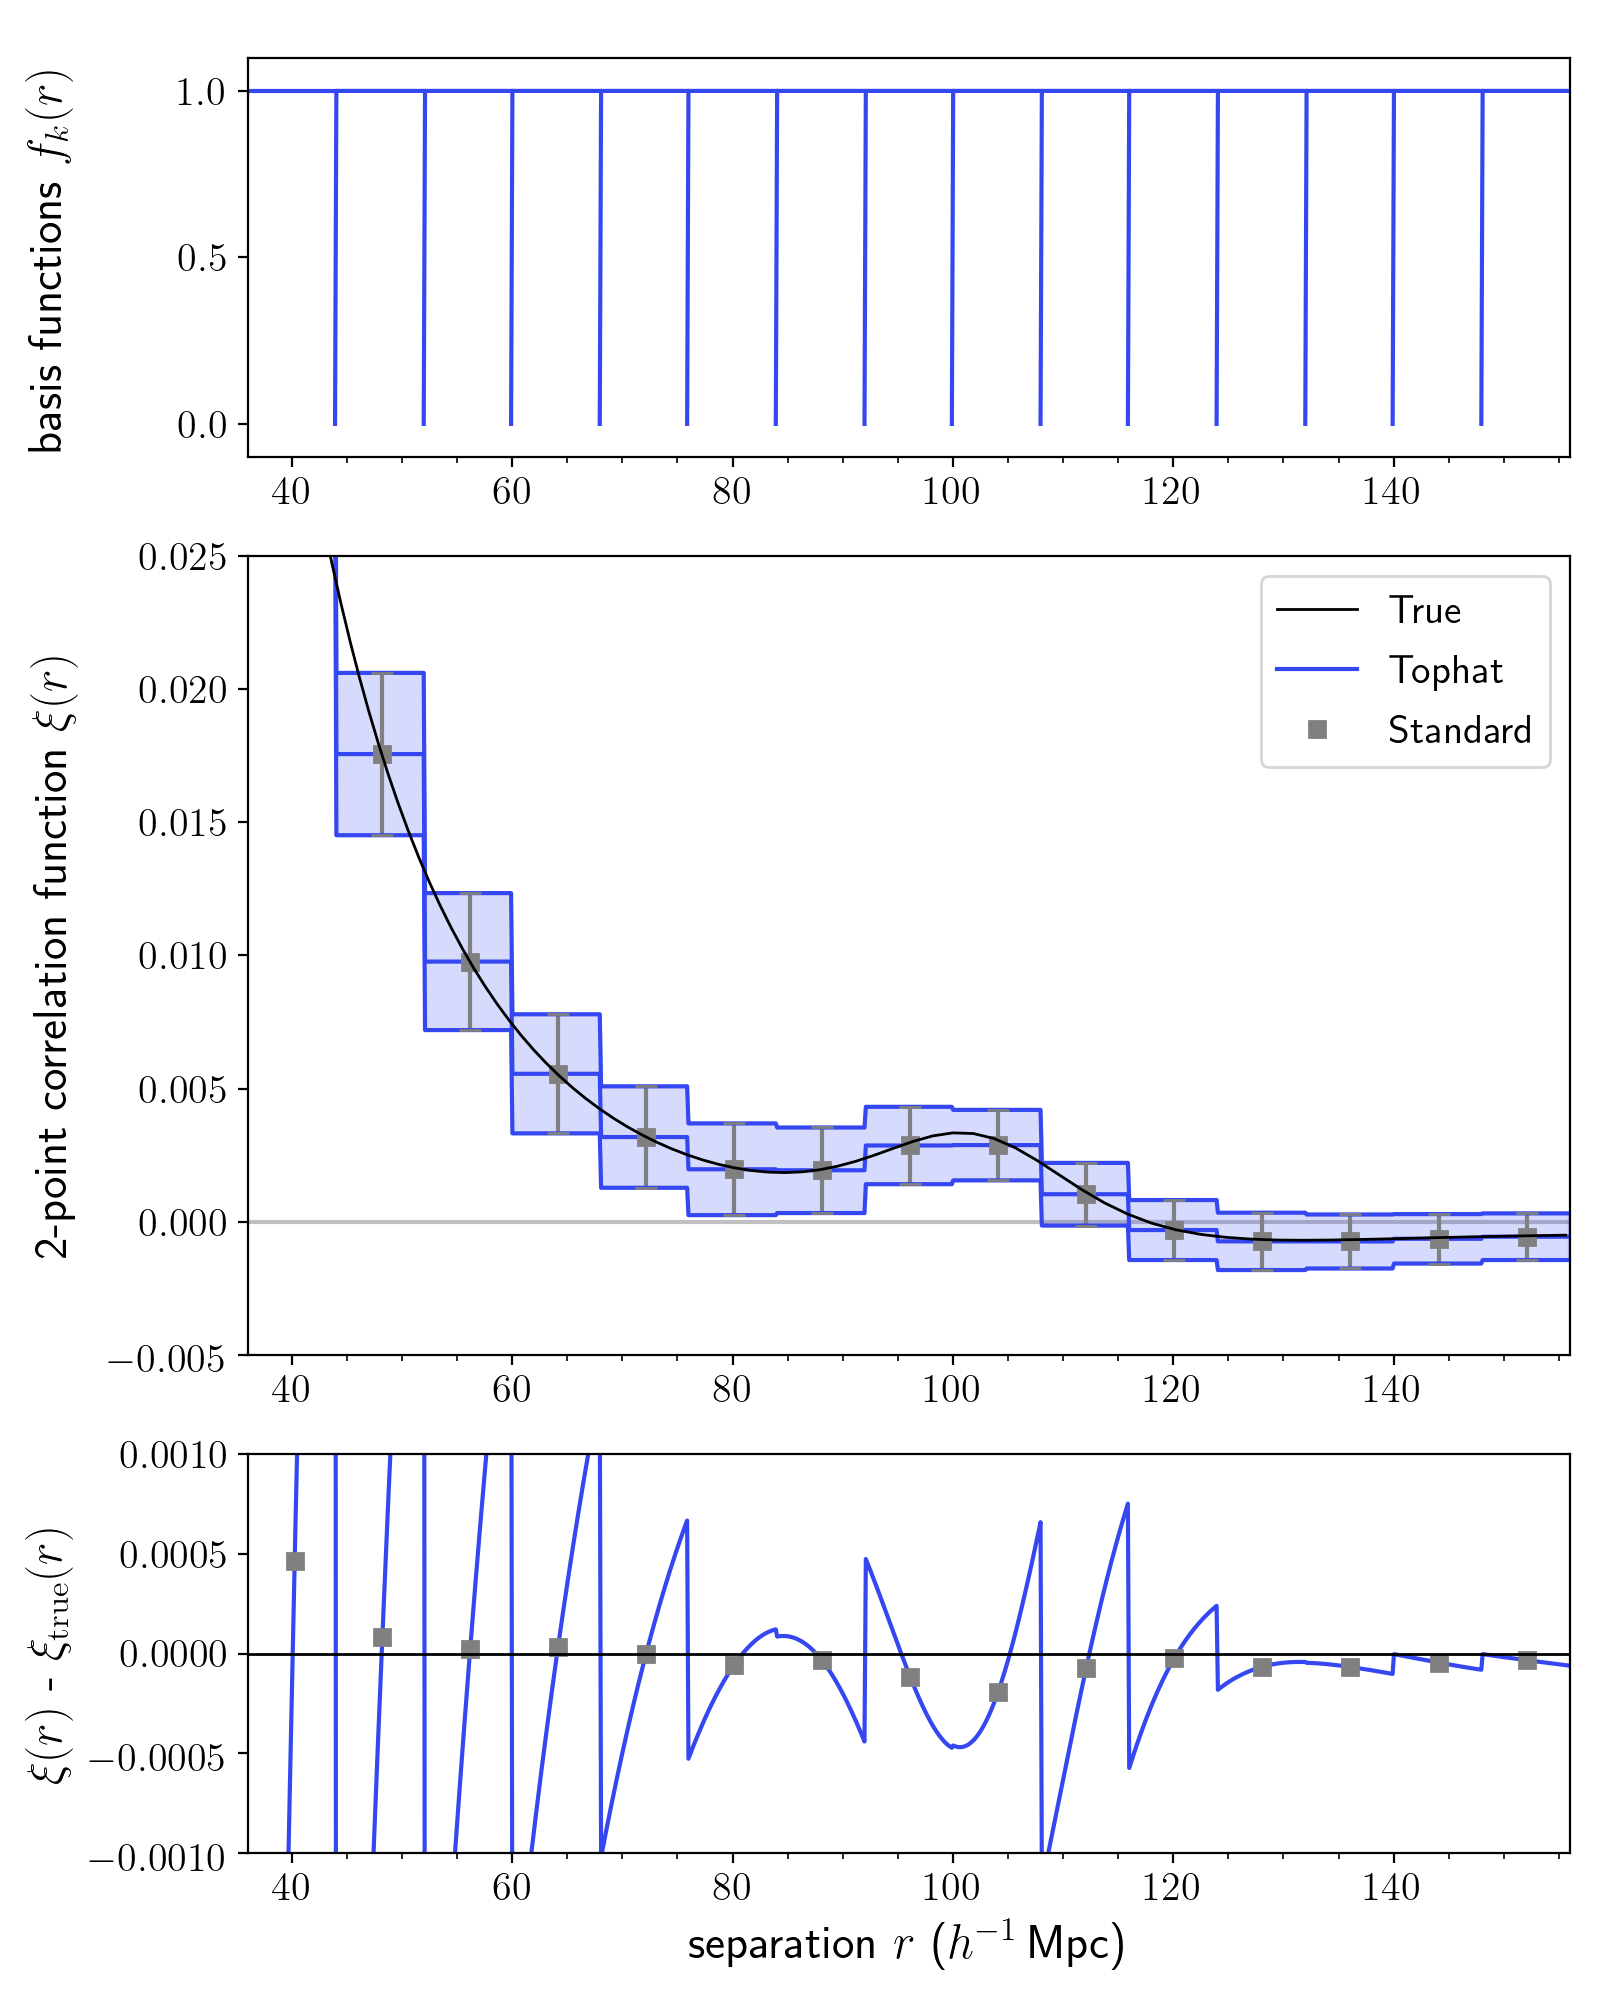
\includegraphics[width=0.8\textwidth]{xicomparison_2e-4_tophat8_theory8}
    \caption{A comparison between \est with a tophat basis (thin blue lines) and the standard estimator (grey squares). The top panel shows the basis functions used for the tophat estimator. The middle panel shows the mean of the estimated correlation functions for 1000 mock catalogs, compared to the true input \cf (thin black line); the shaded region and error bars are the standard deviation of the \cf estimate. The lower panel shows the absolute error between the estimate and true \cf. \Est with a tophat basis is exactly equivalent to the standard estimator, but in a continuous form, emphasizing the fact that binning results in a poor representation of the true \cf.}
    \label{fig:tophat}
\end{figure}
    
We first estimate the correlation function of our mocks using the the standard estimator.
We choose 15 separation ($r$) bins in the range $36 < r < 156$ \hmpc, each with a width of 8 \hmpc; this was found to be the optimal bin width by \cite{Percival2014}, and is standard for two-point analyses.
We apply the estimator to each of our 1000 mock catalogs.
The mean of these estimated correlation functions is shown in Figure~\ref{fig:tophat}; the error bars show the standard deviation of the 1000 mocks in each bin.
We also show the true input correlation function, and the bottom panel shows the absolute error between the estimated and true correlation functions.

There remains an ambiguity in the $r$-value at which to plot the result of the standard estimator. 
The volume-weighted average is often used, or a weighted average depending on the pairs in the bin; this choice propagates to differences in comparing the estimate to models (though at the precision of current surveys these differences are not significant).
Here we plot the standard estimator with the volume-weighted average.

We demonstrate \est with a tophat basis function.
We choose tophat functions with the same locations and widths as the bins used for the standard estimator; these are shown in the top panel of Figure~\ref{fig:tophat}. 
As this estimator computes the \cf in a continuous form, we plot the result as a continuous function at every $r$-value.
In practice, this means choosing a fine grid of $r$-values at which to evaluate $\hat{\xi}(r)$; here we choose 1000 $r$-values across the separation range.
This results in a step function form for the correlation function.
The values of the \cf at each step exactly align with the result of the standard estimator.
In fact, this step function is exactly what the standard estimator is estimating; we have just made explicit the fact that the each estimate applies to the entire bin.
When we look at the error with respect to the truth (bottom panel), the error blows up at the edges of each bin, where the continuous estimate deviates most significantly from the truth.
\new{We recognize that in typical analyses one does not consider the error across the entire bin as shown; rather, one compares the \cf in the bin at some effective $r$-value to a model evaluated at that value.
However, we show the tophat errors here to emphasize  how the standard binned estimator is a poor representation of the true \cf.}

\subsection{Demonstration using Spline Basis Functions}
\label{sec:spline}

A natural extension of tophat basis functions is the B-spline.
B-splines of order $n$ are piecewise polynomials of order $n-1$; they constitute the basis functions for spline interpolation \citep{deBoor1987}.
They have the nice property that the functions and their derivatives can be continuous, depending on the order; \new{this might be important in inference contexts where it is useful to have differentiable models with respect to the parameters of interest, and generally aligns with our belief that physical models of the universe are analytic (i.e. have derivatives of all orders).}
Additionally, B-splines are well-localized, which provides a more direct comparison to the typical tophat basis (which is entirely localized).
For this demonstration we use fourth-order B-splines, which constitute the set of basis functions for a cubic spline, as they are the lowest-order spline to have a continuous first derivative.

We compare the estimator with a cubic-spline basis to the \new{\LS estimator, both in the standard binned representation and reformulated as continuous functions using a tophat basis;} the results are shown in Figure~\ref{fig:spline}.
The basis functions are shown in the top panel of the figure.
We use the same tophat basis as above.
For the cubic-spline basis, we use the same $r$-range and number of basis functions, and knots chosen to evenly span the range. 
The cubic-spline bases on the edge have different shapes such that they remain normalized; we note that generally, one should choose the basis functions such that the \cf range of interest does not depend on the range of the basis functions.

\new{The middle panel shows that \est} using the cubic-spline basis clearly produces a better fit to the true correlation function in its shape and smoothness at every point across the scale range, compared to the estimator using the tophat basis.
The bottom panel shows the error with respect to the truth; the \new{cubic-spline estimator is similar in accuracy}, and directly comparable to the truth (or model) at every scale.
On the other hand, in order to compare the binned \cf to a model, one must integrate the model over the bin range, though in practice the model is often just evaluated at the effective $r$ of each bin.

This comparison demonstrates that there exist other sets of basis functions that produce better representations of the data compared to the standard tophat/binned estimator.
The choice of a high-order spline may be useful for cases in which one wants a mostly localized yet representative estimate of the \cf, or smooth derivatives.
Generally, the choice of basis functions should be tailored to the scientific goal; in the next section we explore the case of a BAO analysis.

\begin{figure}[ht]
    \centering
        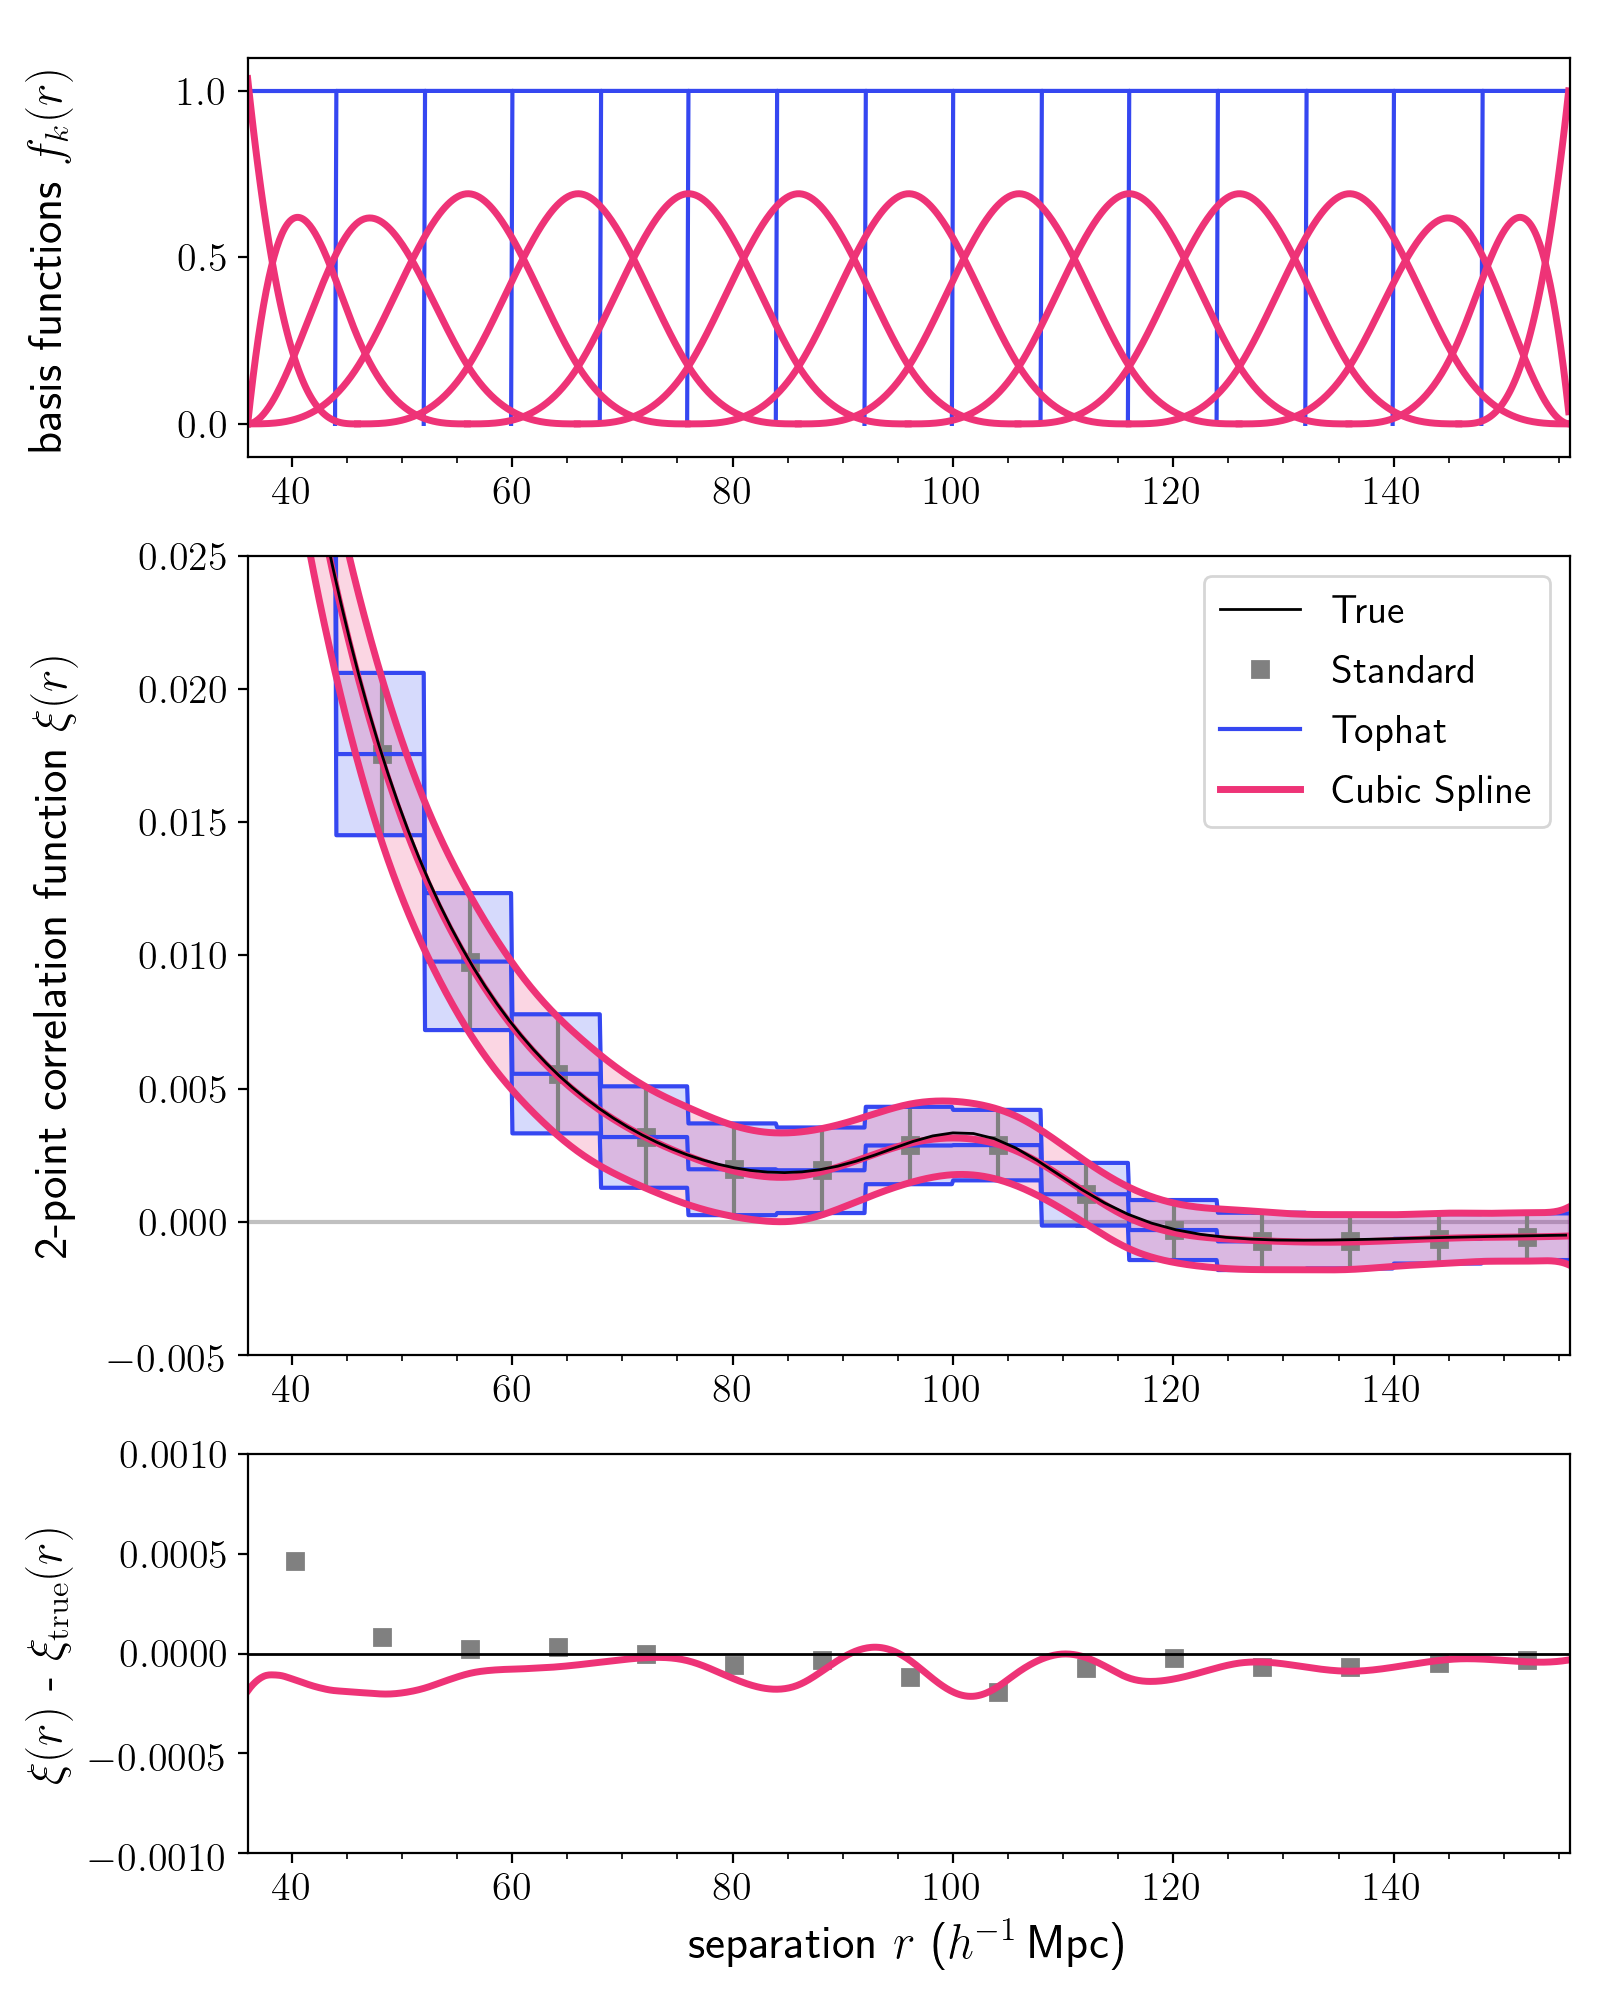
\includegraphics[width=0.8\textwidth]{xicomparison_2e-4_tophat8_spline}
        \caption{\new{A demonstration of} \est with cubic-spline basis functions (thick red). \new{We compare the cubic-spline estimate to the standard binned Landy--Szalay estimate (grey squares), and to the continuous-function estimate with a tophat function (thin blue).} The top panel shows the basis functions used for each measurement. The middle panel shows the mean of the estimated correlation functions for each of the 1000 mock catalogs compared to the true input \cf (thin black); the shaded region \new{and error bars} are the standard deviation. The lower panel shows the absolute error between the estimate and true \cf; \new{we do not show the tophat error for clarity}. It is clear that the spline basis function results in a correlation function that is a better representation of the true \cf in its shape and smoothness.}
        \label{fig:spline}
    \end{figure}    

\subsection{BAO Scale Estimation Test}
\label{sec:bao}

The measurement of the baryon acoustic oscillation (BAO) scale provides an apt use case for our estimator.
The BAO feature is a peak in clustering on large scales, $\sim$150 Mpc ($\sim$100\hmpc), making it less sensitive to small-scale astrophysical effects.
It is one of the best tools for constraining cosmological models, in particular the distance--redshift relation \citep{Cole2005, Eisenstein2005, Kazin2010, Anderson2012, Anderson2014, Alam2017}.

We base our BAO analysis on the method of the BOSS DR10 and 11 analysis \citep{Anderson2014}.
We estimate the spherically averaged 3-dimensional correlation function, $\hat{\xi}(r)$, where $r$ is the separation between pairs.
(BAO analyses are typically done in redshift space, estimating $\hat{\xi}(s)$, where $s$ is the redshift-space separation between pairs, but here we are using a periodic box in which we know the true galaxy positions, so we just use the real-space distance $r$.)
In order to extract information about the baryon acoustic feature from galaxy clustering, we must choose a fiducial cosmological model to convert redshifts to distances.
If we choose an incorrect model, the scales in the power spectrum will be dilated, so the oscillation wavelength{\emdash}and thus the BAO peak position{\emdash}will be shifted.
We can model this shift as a scale dilation parameter, $\alpha$, which is a function of the relevant distance scales in the true and fiducial cosmologies, defined as
\begin{equation} \label{eq:alpha}
\alpha = \Bigg( \frac{D_\mathrm{A}(z)}{D_\mathrm{A}^{\text{mod}}(z)} \Bigg)^{2/3} \Bigg( \frac{H^{\text{mod}}(z)}{H(z)} \Bigg)^{1/3} \Bigg( \frac{r_\mathrm{s}^{\text{mod}}}{r_\mathrm{s}} \Bigg) ~,
\end{equation}
where $D_\mathrm{A}$ is the angular diameter distance, $H$ is the Hubble parameter, $z$ is the redshift, $r_\mathrm{s}$ is the sound horizon scale at the drag epoch, and the superscript ``$\text{mod}$'' denotes the value for the chosen fiducial model (the non-superscripted parameters are the true values).
Qualitatively, if the fit prefers $\alpha>1$, this suggests the true position of the BAO peak is at a smaller scale than in the fiducial model, whereas if $\alpha<1$, the peak is at a larger scale.
With isotropic analyses, there is a degeneracy between $D_\mathrm{A}$ and $H$, so typically a combination of these values is reported; the degeneracy can be broken with anisotropic BAO analyses.
Our estimator could straightforwardly perform an estimate of the anisotropic correlation function, but for demonstration purposes we perform an isotropic analysis here and focus on the recovered value of $\alpha$.

In standard practice, the fitting function used to determine the value of $\alpha$ is 
\begin{equation}
\xi^{\mathrm{fit}}(r) = B^2 \xi^{\mathrm{mod}}(\alpha r) + \frac{a_1}{r^2} + \frac{a_2}{r} + a_3 ~,
\end{equation}
where $B$ is a constant that allows for a large-scale bias, and $a_1$, $a_2$, and $a_3$ are nuisance parameters to account for the broadband shape.
A $\chi^2$ fit is performed at intervals of $\Delta \alpha$, with $B$, $a_1$, $a_2$, and $a_3$ as free parameters. 
The resulting value for $\alpha$ is used to derive the actual values of the distance scales of interest.
\new{Typically, analyses have to correct for the broadening of the BAO peak caused by nonlinear growth \citep{Eisenstein2007}; approaches include computing the model with a damping parameter, or performing density-field reconstruction before applying the estimator.
As we use lognormal mocks, we do not need to perform this step, but a realistic analysis must either used a damped model for the basis functions or reconstruct the density field.}

The form of the standard fitting function is well-suited to our estimator, as it is a few-parameter model with a linear combination of terms.
To use our estimator to estimate $\alpha$, we add a term that includes the partial derivative of the model with respect to $\alpha$.
This allows us to have fixed basis functions, and for an initial choice of $\alpha_\mathrm{guess}$, determine the change in this value needed to improve the fit. 
Our fitting function is then
\begin{equation} \label{eq:baoiter_fit}
\xi^\mathrm{fit}(r) = B^2\,\xi^\mathrm{mod}(\alpha_\mathrm{guess}\,r) + C\,k_0\,\frac{\dd \xi^\mathrm{mod}(\alpha_\mathrm{guess}\,r)}{\dd \alpha} + a_1\,\frac{k_1}{r^2} + a_2\,\frac{k_2}{r} + a_3\,k_3 ~,
\end{equation}
where $C$ is an additional coefficient that describes the contribution of the derivative term, and $k_0$, $k_1$, $k_2$, and $k_3$ are constants that determine the initial magnitude of the basis functions.
In this case, the free parameters are $B^2$, $C$, $a_1$, $a_2$, and $a_3$.
Note that in theory the choice of $k_i$ values shouldn't matter as the estimator is affine invariant (see Appendix~\ref{sec:affine}), but in practice reasonable choices are important for stability.
The adopted $k_i$ values are noted in Appendix~\ref{sec:baoiter}.

\begin{figure}[t]
    \centering
    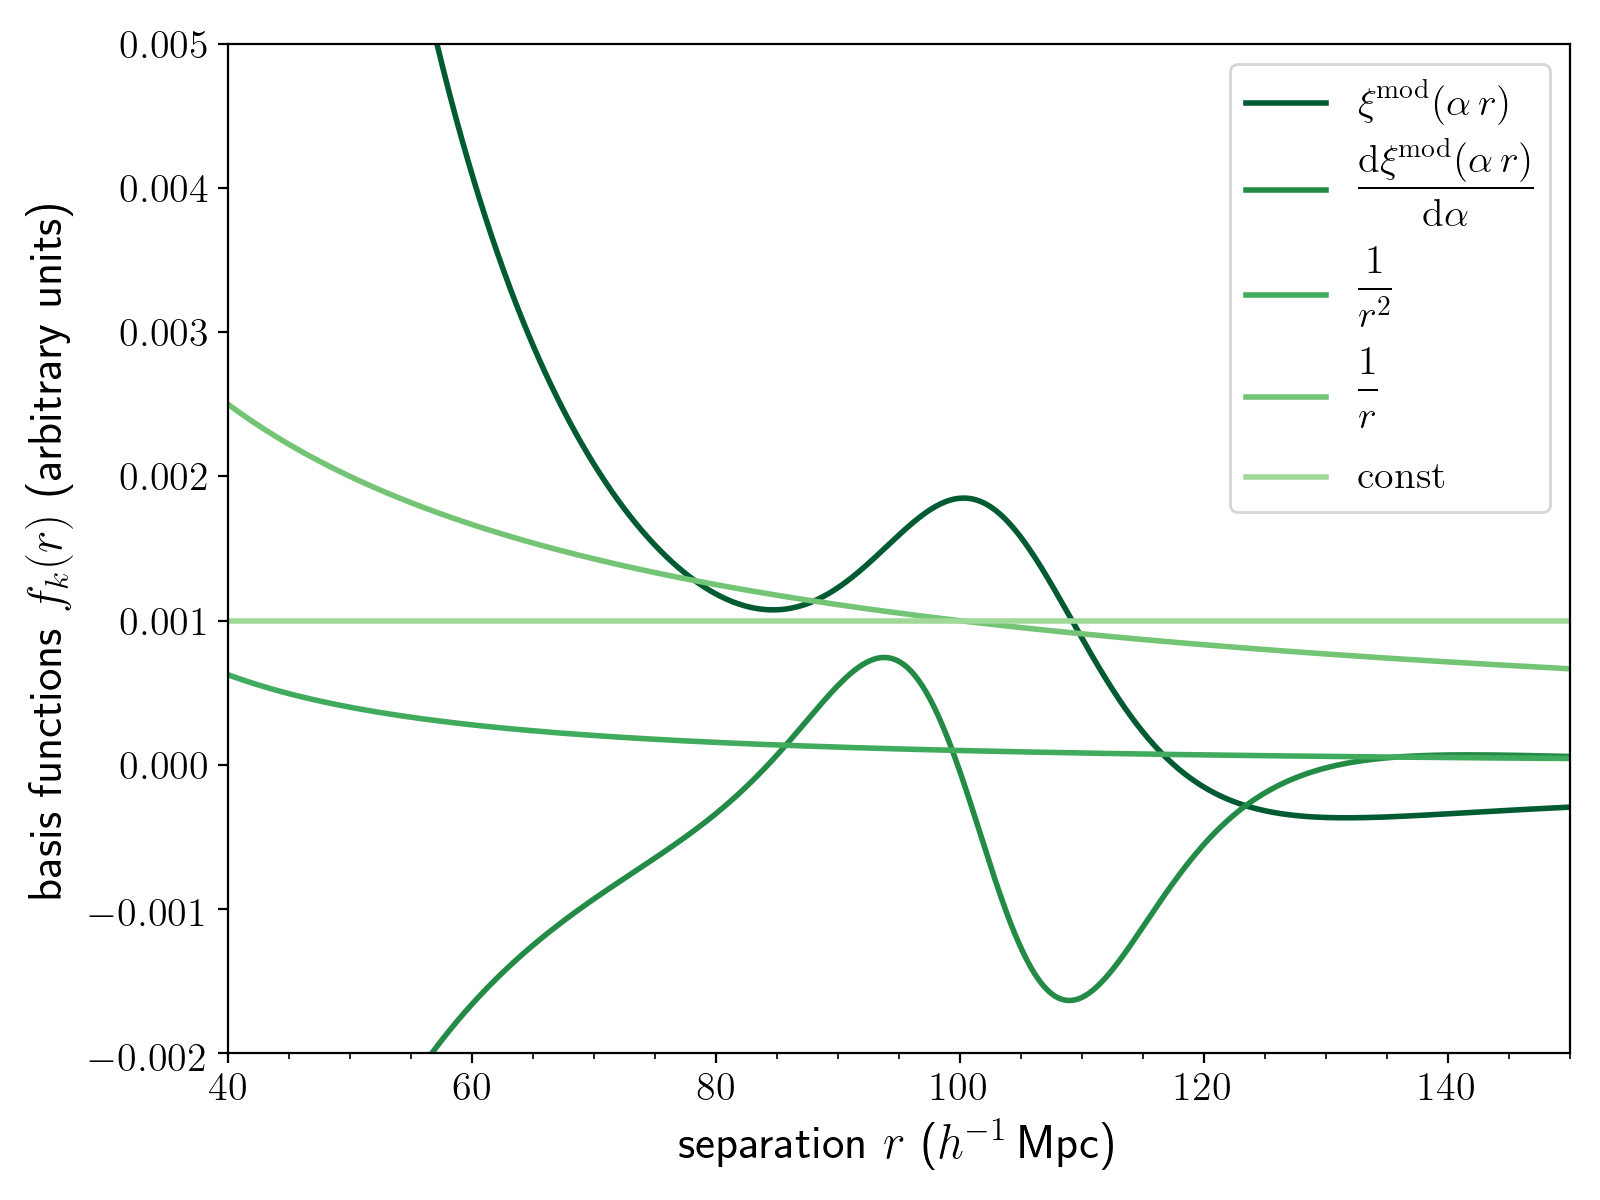
\includegraphics[width=0.8\textwidth]{bao_bases}
    \caption{The set of basis functions used to fit for the BAO scale using our estimator. The $\xi^\mathrm{mod}(\alpha\,r)$ term (darkest green) is the correlation function computed using fiducial model, with some scale dilation $\alpha$. The derivative term (second-to-darkest green) is the derivative of this model with respect to $\alpha$, which allows for the direct estimation of this parameter. The other three terms (lighter greens) are nuisance parameters to fit the broadband shape.}
    \label{fig:bao_bases}
\end{figure}

To use the estimator for a BAO measurement, we input these five terms as the five basis functions of our estimator.
The estimator outputs an amplitude vector $\bld{\hat a}$ as described in Section~\ref{sec:est}, which describes the contribution of each basis function{\emdash}precisely the values of the free parameters, scaled by $k_i$.
From the value of $C$, we can determine our estimate of the scale dilation parameter, $\hat{\alpha}$, as $\hat{\alpha} = \alpha_\mathrm{guess} + C\,k_0$, based on the definition of finite derivatives. 
With this formulation, a value of $C=0$ indicates that the current $\alpha_\mathrm{guess}$ gives the best fit to the data (given the chosen cosmological model), while nonzero values give the magnitude and direction of the necessary change in the scale dilation parameter to optimally fit the data.
In practice, we apply an iterative procedure to converge at our best estimate $\hat{\alpha}$; this procedure and other implementation details are described in Appendix~\ref{sec:baoiter}.

We demonstrate this method using our set of lognormal mock catalogs.
We construct a recovery test following that in \cite{Hinton2019}.
We assume the fiducial cosmological model used in \cite{Beutler2017}: $\Omega_{\text{m}} = 0.31$, $h = 0.676$, $\Omega_{\text{b}} = 0.04814$, $n_s = 0.97$. 
As we know the cosmology used for our mock catalogs, we can compute the true value of the scale dilation parameter, $\alpha_{\text{true}}=0.9987$.
(Here our choice of fiducial model happened to be close to the true model, so our $\alpha_{\text{true}}$ is very close to 1; this is typical, as our cosmological model is fairly well-constrained.)
With this fiducial model, we can construct the basis functions for our estimator; these are shown (with $\alpha=1$ and arbitrary scaling) in Figure~\ref{fig:bao_bases}.

\begin{figure}[t]
\centering
    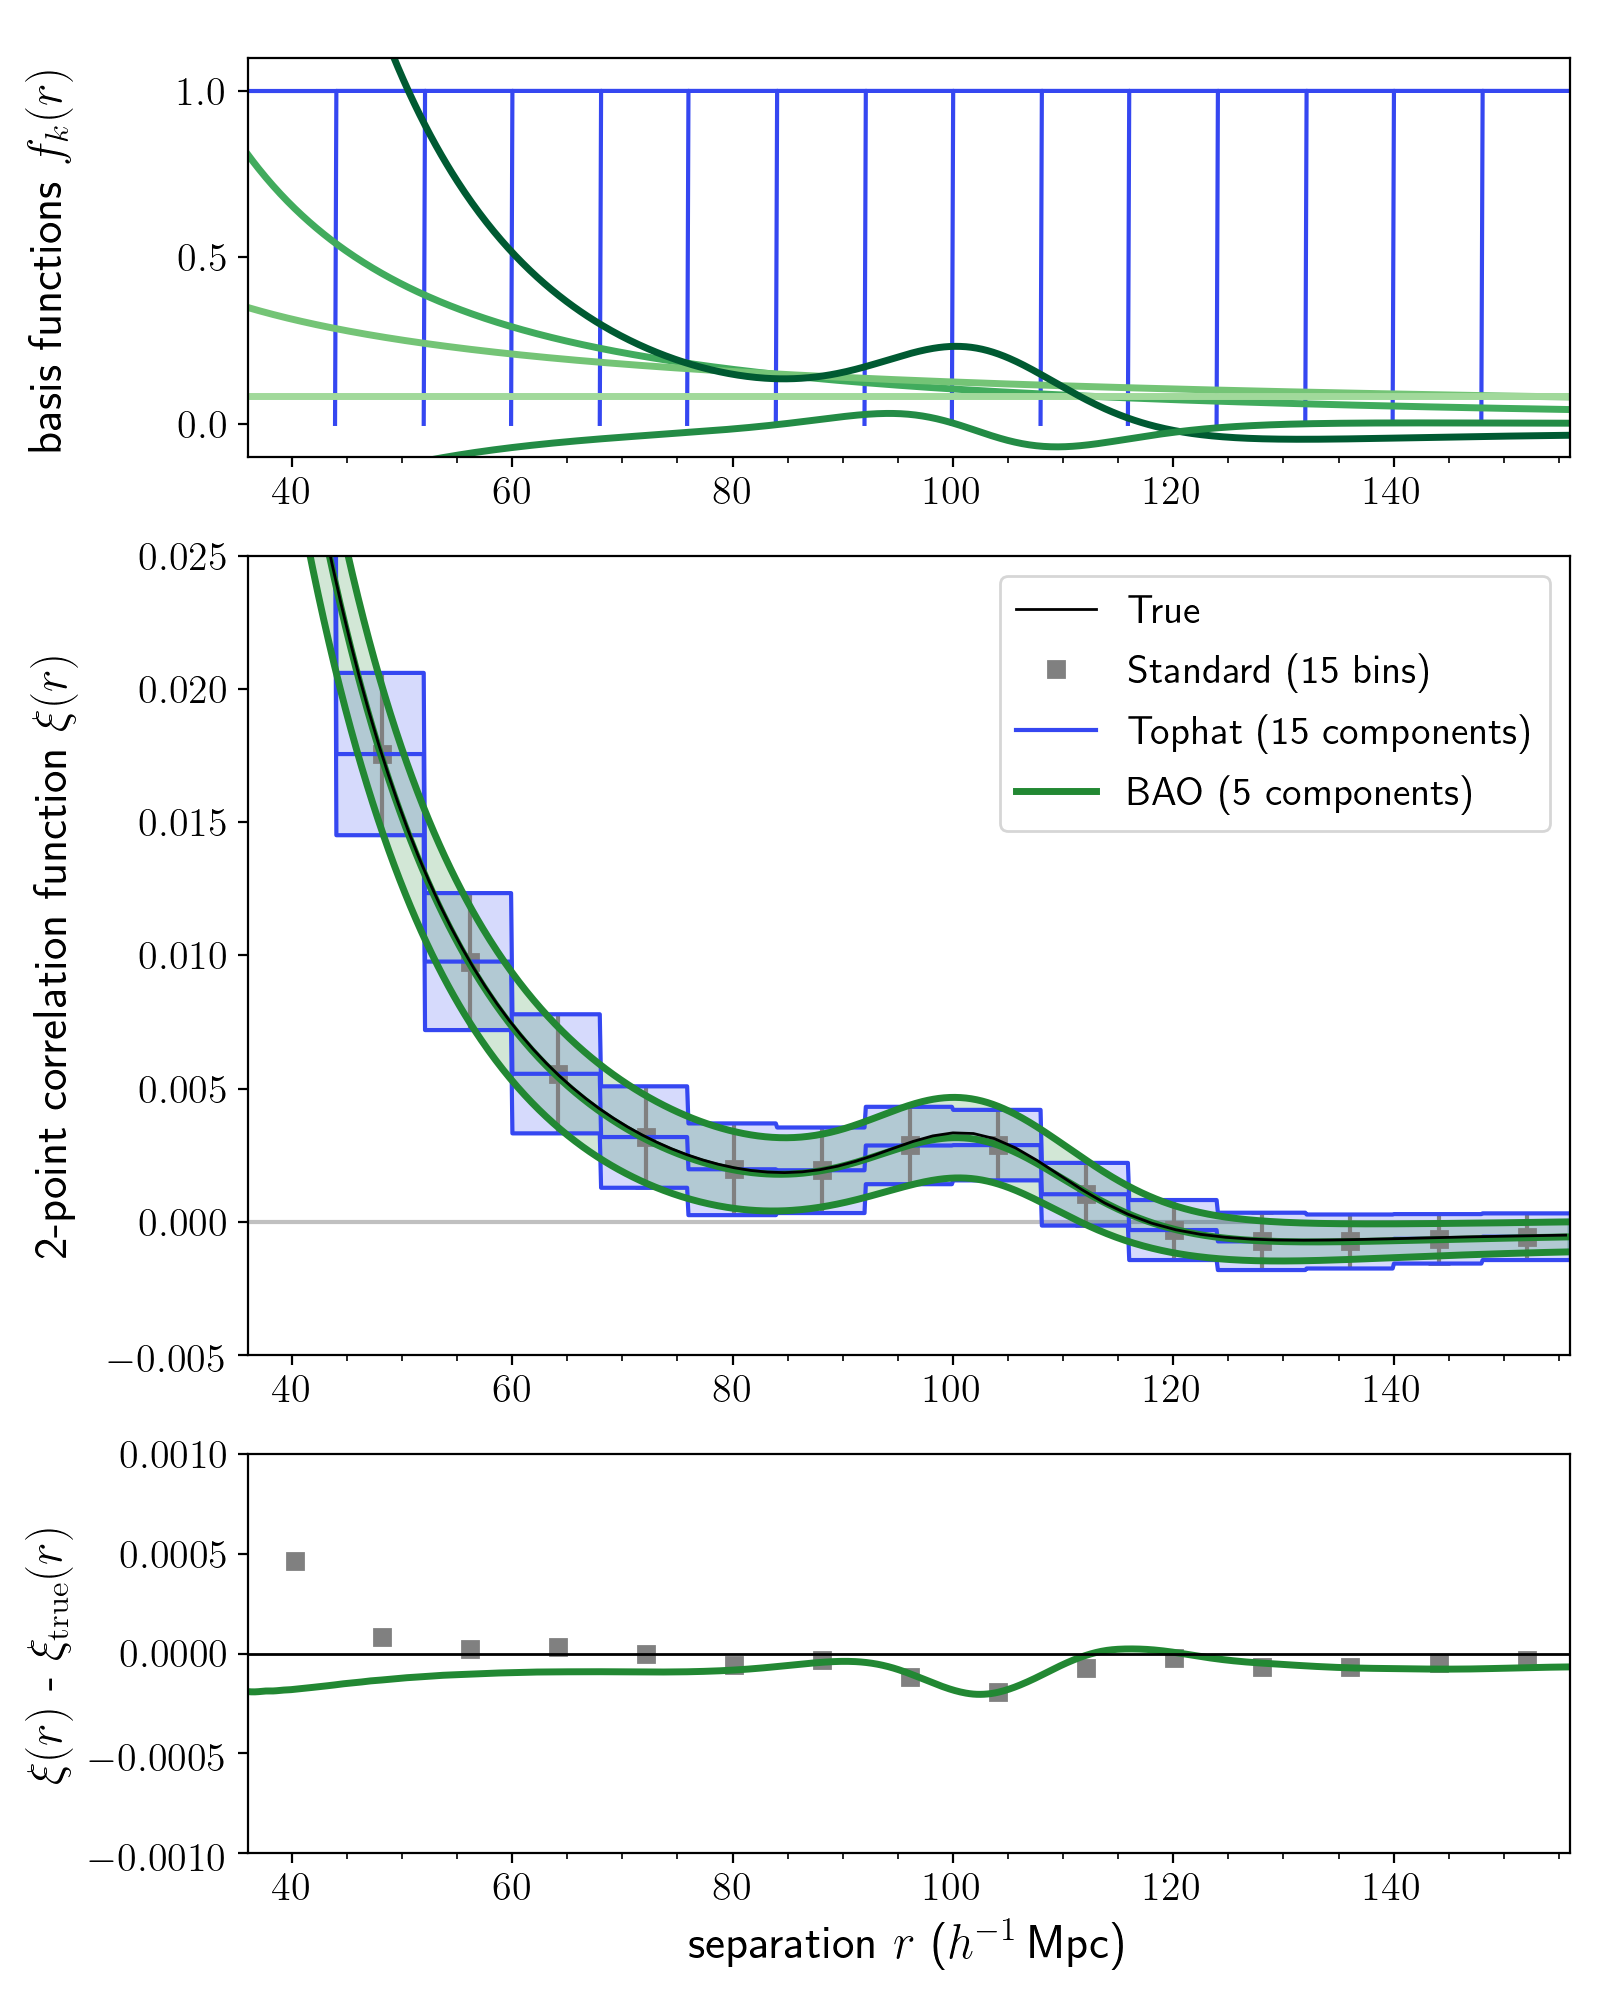
\includegraphics[width=0.8\textwidth]{xicomparison_2e-4_tophat8_baoiter}
    \caption{Estimation of the correlation function using \est with basis functions based on the BAO fitting function (thick green; same as in Figure~\ref{fig:bao_bases}, with arbitrary scaling). \new{We compare this to the standard binned Landy--Szalay estimator (grey squares), and to} \est with a tophat function (thin blue). \new{The panels are the same as in Figure~\ref{fig:spline}.}}
    \label{fig:bao}
\end{figure}

We apply our iterative estimation procedure to each of the 1000 mocks; the mean of the resulting estimates for the correlation function is shown in Figure~\ref{fig:bao}.
We show the BAO basis functions in the top panel, as in Figure~\ref{fig:bao_bases}.
We compare \est using the BAO bases with that using tophat bases, as in the previous sections; \new{we also show the standard representation of the binned estimator.}
The correlation function estimated with the BAO bases clearly produces a more representative estimate at all scales.
The estimate is also smoother than that produced using the cubic-spline basis functions (Figure~\ref{fig:spline}).
More importantly, it is scientifically motivated: the estimator produces the relative contributions of the terms of the BAO fitting functions.
\new{This gives us the best-fit model for each of the 1000 mock catalogs, without the need for intermediate binning and fitting steps, and} allows us to directly estimate the best-fit value of $\alpha$ for each one.
The median estimate of the recovered scale dilation parameter is $\alpha=0.9975 \pm 0.0290$, where the uncertainty is based on the 16th and 84th percentiles; our estimate is very close to the true value of $\alpha = 0.9987$.

We emphasize that the BAO-based estimate requires only five components, while the tophat basis requires 15 components (or bins, in the standard approach) in the same scale range.
This is critical for the efficient computation of a precise covariance matrix, as the errors depend on the number of components used for the estimate, as described in Section~\ref{sec:covariance}.
\Est with the BAO basis functions could reduce the number of mocks needed to achieve the same precision by a factor of a few to an order of magnitude; as these expensive cosmological simulations are currently the limiting step in two-point analyses, this could be highly impactful.

We note that these basis functions are significantly different than the tophat or B-spline bases previously explored.
One important difference is that they are not localized.
This means that data at all scales could contribute to all basis functions.
It is then critical for the investigator to ensure that the range of scales chosen is reasonable for the scientific problem at hand and that the final estimate of the parameter of interest does not depend on the details of this choice.
The nonlocality also means that the covariance matrix between the components will have a very different structure than typical binned covariance matrices.
We return to this issue in Section~\ref{sec:covariance}.


\section{Technical Details}

\subsection{Affine Invariance of the Estimator}\label{sec:affine}

The estimate of the \cf with \est should not depend on the scaling of the chosen basis functions.
Thus we expect \est to be invariant under affine transformations of the basis functions, meaning transformations that preserve collinearity and distance ratios; the following demonstrates this affine invariance.

We represent the affine transformation by an invertible transformation matrix $\bld{M}$ that modifies the basis functions $\ff$, such that 
\begin{equation}
\ff' \leftarrow \bld{M}\,\ff ~,
\end{equation}
where the prime indicates our affine-transformed basis.
We choose $\bld{M}$ to be invertible to ensure the two bases have the same expressive capacity.
Then in the primed basis, the pair counts become
\begin{eqnarray}\displaystyle
\vv{DD}' &=& \adjustlimits \sum_{n} \sum_{n'} \ff_{n n'}' = \sum_{n n'} \bld{M}\,\ff_{n n'} = \bld{M}\,\vv{DD}
\\
\vv{DR}' &=& \sum_{n} \sum_{m} \ff_{n m}' = \sum_{n m} \bld{M}\,\ff_{n m} = \bld{M}\,\vv{DR}
\\
\vv{RR}' &=& \adjustlimits \sum_{m} \sum_{m'} \ff_{m m'}' = \sum_{m m'} \bld{M}\,\ff_{m m'} = \bld{M}\,\vv{RR} ~,
\end{eqnarray}
where we use the shorthand $\ff_{i j} = \ff(\GG{i j})$ and we have omitted the normalization factors for clarity.
In the last step, we have factored $\bld{M}$ out of the summation and written the primed projection vectors in terms of the unprimed vectors. 

For the random--random tensor we have
\begin{eqnarray}\displaystyle
\TT{RR}' &=& \adjustlimits \sum_{m} \sum_{m'} (\bld{M}\,\ff_{m m'}) \cdot (\bld{M}\,\ff_{m m'})\T \\
&=& \bld{M}\left[ \adjustlimits \sum_{m} \sum_{m'} \ff_{m m'} \cdot \ff_{m m'}\T \right] \bld{M}\T \\
&=& \bld{M}\,\TT{RR}\,\bld{M}\T ~.
\end{eqnarray}
Then the amplitudes in the primed basis become
\begin{eqnarray}\displaystyle
\bld{\hat a}' &=& \TT{RR}\invp \cdot (\vv{DD}' - 2\,\vv{DR}' + \vv{RR}') \\
\bld{\hat a}' &=& [\bld{M} \TT{RR} \bld{M}\T]\inv \cdot [\bld{M}\,\vv{DD} - 2\,\bld{M}\,\vv{DR} + \bld{M}\,\vv{RR}] \\
&=& (\bld{M}\T)\inv \, \TT{RR}\inv \, \bld{M}\inv \cdot \bld{M}\,[\vv{DD} - 2\,\vv{DR} + \vv{RR}] \\
&=& (\bld{M}\T)\inv \, \TT{RR}\inv \cdot [\vv{DD} - 2\,\vv{DR} + \vv{RR}] \\
&=& (\bld{M}\T)\inv \, \bld{\hat a}
\end{eqnarray}
and the estimator $\bld{\hat{\xi}}'$ in the primed basis, using the shorthand $\hat{\xi}_{\ell \ell'} = \hat{\xi}(\GG{\ell \ell'})$, is 
\begin{eqnarray}\displaystyle
\hat{\xi}_{\ell \ell'}' &=& \bld{\hat a}\Tp \cdot \ff_{\ell \ell'} \\
\hat{\xi}_{\ell \ell'}' &=& [(\bld{M}\T)\inv \, \bld{\hat a}]\T \cdot (\bld{M}\,\ff_{\ell \ell'}) \\
&=& \bld{\hat a}\T \, [(M\inv)\T]\T \cdot (\bld{M}\,\ff_{\ell \ell'}) \\
&=& \bld{\hat a}\T \, \bld{M}\inv \cdot \bld{M}\,\ff_{\ell \ell'} \\
&=& \bld{\hat a}\T \cdot \ff_{\ell \ell'} \\
&=& \hat{\xi}_{\ell \ell'} ~.
\end{eqnarray}
Thus after an affine transformation of the basis function, the resulting estimator is equivalent to the estimator in the original basis.
The method is shown to be affine invariant.


\subsection{Computing the Random--Random Terms Analytically}\label{sec:analytic}

The autocorrelation of the random catalog is meant to approximate the autocorrelation of the window function. 
When we have a periodic cube, we can compute this $\vv{RR}$ term analytically in the standard approach to correlation function estimation.
Here we derive this, and then derive the equivalent for our continuous-basis $\vv{RR}$ and $\TT{RR}$ terms.

Our goal is to estimate the normalized number of pairs in a periodic cubic volume filled uniformly with tracers, $\vv{RR}^\mathrm{ana}$. 
We first consider an annulus indexed by $k$ around a single galaxy, with radial edges $g_k$ and $h_k$. 
This annulus has a volume $V_k$.
Taking the box to have an average number density $\bar{n}$, the number of galaxies expected in the annulus is $N_k = V_k \, \bar{n}$, and thus our selected galaxy contributes $N_k$ pairs to the count.   
We do this for each of the $\NN{R}-1$ other galaxies, and after including a factor of $\frac{1}{2}$ to account for the fact that this double counts pairs, we find a total pair count of $\frac{1}{2} \, (\NN{R}-1) \, N_k = \frac{1}{2} \, (\NN{R}-1) \, V_k \, \bar{n}$.
For a cubic volume, $\bar{n} = \NN{R}/L^3$, so our final pair count for the annulus is  $\frac{1}{2} \, \NN{R}(\NN{R}-1) \, V_k \, / L^3$.
We want the normalized pair counts, so we divide by the number of unique pairs, $\NN{R}(\NN{R}-1)/2$; this cancels out all instances of $\NN{R}$, as it should as this approximation is not actually using random catalog, and leaves us with $\left[ \vv{RR}^\mathrm{ana} \right]_k = V_k / L^3 ~.$

We now need to compute $V_k$; for hard-edged radial bins, we can compute $V_k$ simply as the difference between spherical volumes. 
We can represent this more generally as an integral,
\begin{equation} \label{eq:vol_tophat}
V_k = \int_{g_k}^{h_k} dV = 4\pi \int_{g_k}^{h_k} r^2 \, dr ~,
\end{equation}
where we assume spherical symmetry.
We can generalize this to any basis function $f_k(r)$ that is only a function of $r$,
\begin{equation}
V_k = 4\pi  \int_{g_k}^{h_k} f_k(r) \, r^2 \, dr ~,
\end{equation}
where $k$ is now the index of the basis functions.
This reduces to \eqt{eq:vol_tophat} when $f_k(r)$ is the tophat function (returning 1 or 0 depending on whether or not $r$ falls between $g_k$ and $h_k$).

Combining the above equations gives us our full generalized analytic random--random projection vector $\vv{RR}^\mathrm{ana}$, which has elements
\begin{equation}
\left[ \vv{RR}^\mathrm{ana} \right]_k = \frac{1}{L^3} \, 4\pi \, \int_{r_\mathrm{min}}^{r_\mathrm{max}} f_k(r) \, r^2 \, dr ~,
\end{equation}
where we are now integrating over all values of $r$ we are interested in from some $r_\mathrm{min}$ to $r_\mathrm{max}$.
(For non-localized basis functions, the fully correct thing would be to integrate from $-\infty$ to $\infty$, though some bounds must be chosen in practice.)

Based on the definition of $\TT{RR}$ in \eqt{eq:Trr} as the sum of outer products of the basis function vectors and their transposes, the elements of the analytic random--random tensor $\TT{RR}^\mathrm{ana}$ can be written as
\begin{equation}
\left[ \TT{RR}^\mathrm{ana} \right]_{kk'} = \frac{1}{L^3} \, 4\pi \, \int_{r_\mathrm{min}}^{r_\mathrm{max}} f_k(r) \, f_{k'}(r) \, r^2 \, dr ~.
\end{equation}
This could be further generalized to account for basis functions that take properties other than pair separation as input.

For the periodic box case, we can think about the cross-correlation term $\vv{DR}$ similarly; now we are taking each of the $\NN{D}$ galaxies in the data catalog and estimating the normalized pair counts of their cross-correlation with a theoretical random catalog.
It turns out that the resulting projection vector for the cross-correlation is exactly the same as for the random autocorrelation, $\vv{RR}^\mathrm{ana}  = \vv{DR}^\mathrm{ana}$.
Thus the Landy-Szalay estimator reduces to the natural estimator, and we can compute the analytic amplitudes $\bld{\hat a}^{\mathrm{ana}}$ for \est as
\begin{equation}
\bld{\hat a}^{\mathrm{ana}} = \left[ \TT{RR}^\mathrm{ana} \right]\inv \cdot \left( \vv{DD} - \vv{RR}^\mathrm{ana} \right) ~.
\end{equation}
Finally, we use these amplitudes to compute the correlation function $\bld{\hat{\xi}}^{\mathrm{ana}}$ as before in \eqt{eq:xi_proj}.

This analytic form for the continuous estimator could be extended to basis functions that depend on other tracer properties in addition to pair separation.
In this case, one would have to integrate over these axes as well, but the idea is the same.


\subsection{Implementation of Estimation with BAO Basis Functions}\label{sec:baoiter}

\subsubsection{Iterative Procedure}

\Est can be used to measure the baryon acoustic oscillation (BAO) scale by choosing the basis functions to terms of a BAO fitting function, as described in Section~\ref{sec:bao} and shown in Figures~\ref{fig:bao_bases} and~\ref{fig:bao}.
For this application, we need to choose a fiducial cosmology for our bases, which will be offset from the true cosmology.
This offset can be encoded by a scale dilation parameter $\alpha$, which contains the information about the BAO scale; see \eqt{eq:alpha}. 
As our fitting function requires a fiducial model and an initial guess of this parameter, $\alpha_\mathrm{guess}$, and then determines the change needed, an iterative procedure is needed to converge to the best-fit value.

We start with assuming that we have chosen our fiducial model to match our true cosmology (we in all likelihood have not, but it's not a bad initial guess), giving us an initial $\alpha_\mathrm{guess} = 1.0$. 
We then apply \est to perform the measurement, and obtain the magnitude of the projection $C$ for the derivative term in our model as in \eqt{eq:baoiter_fit}. 
This gives us our estimate $\hat{\alpha}$ of the scale dilation parameter from this initial model; for the $i$th iteration, we have
\begin{equation}
    \hat{\alpha}_{i} = \alpha_{\mathrm{guess},i} + C_i \, k_0 ~,
\end{equation}
where $k_0$ is the chosen scaling parameter for the derivative basis function as in \eqt{eq:baoiter_fit}.

We choose the convergence criterion to be when the fractional change in $\hat{\alpha}$ between subsequent iterations falls below a threshold, $c_\mathrm{thresh}$,
\begin{equation}
    \left| \frac{\hat{\alpha}_i - \hat{\alpha}_{i-1}}{\hat{\alpha}_i} \right| < c_\mathrm{thresh} ~.
\end{equation}
For our application we choose $c_\mathrm{thresh} = 0.00001$.

To achieve convergence, we need to be careful in choosing our next $\alpha_{\mathrm{guess},i}$.
If it is far from the best estimate, $C_i$ will be large, and our resulting estimate $\hat{\alpha}_{i}$ will be inaccurate.
We thus include a damping parameter $\eta$ between 0 and 1 to improve our convergence.
Our next guess is then
\begin{equation}
    \alpha_{\mathrm{guess},i+1} \leftarrow \alpha_{\mathrm{guess},i} + \eta\,C_i\,k_0 ~.
\end{equation}
The choice of $\eta$ is important for stability and speed of convergence; too large a value can lead to a back-and-forth cycle in which the result hops between two values and never converges, and too small a value would make convergence take a very long time.
In our application, we start with $\eta=0.5$.
We check if our estimate is jumping over the true value by checking if the error changes sign; if it does, we reduce $\eta$ by a factor of $0.75$.

\subsubsection{Implementation Details}

We implement the partial derivative in the fitting function of \eqt{eq:baoiter_fit} as a finite difference between model with the our chosen value of $\alpha_\mathrm{guess}$, and the model with a value shifted by a small $\Delta \alpha$,
\begin{equation}
    \frac{\dd \xi^\mathrm{mod}(\alpha \, r)}{\dd \alpha} \leftarrow \frac{\xi^\mathrm{mod}(\alpha_\mathrm{guess} \, r) - \xi^\mathrm{mod}((\alpha_\mathrm{guess} + \Delta \alpha) \, r)}{\Delta \alpha} ~.
\end{equation}
In our implementation we take $\Delta \alpha = 0.001$; we have checked that our results are insensitive to this choice.

We choose the magnitudes of the basis functions $k$ to set them at similar scales, providing improved stability.
We use the values $k_0=0.1$, $k_1=10.0$, $k_2=0.1$, and $k_3=0.001$, though we check that the results are insensitive to choices near these values.




\section{Discussion} \label{sec:discuss}

\subsection{Estimator Usage and Limitations}

In this \documentname we have performed a few example applications of \est (for others see Section~\ref{sec:applications_cfe}); these demonstrate the problems solved and opportunities created with the estimator.
In removing the need for binning, the estimator can produce a much more \textit{representative} correlation function; a mixture of tophats is a very poor representation of the \cf. 
We almost always expect some sort of continuity in the functions we work with; nature does not bin.

One of the problems with binning is that there are choices to be made in bin widths and locations.
We note that our approach does not actually help with these choice issues.
In fact, \est expands investigator choice almost infinitely, as the space of possible basis functions is far larger than the space of possible binnings.
That said, \new{there are ways to make a well-motivated selection of basis functions.
In cases where there is a clear scientific model that can be represented as a linear combination of terms, choosing this will result in the most direct recovery of the parameters of interest (e.g., our BAO estimate in Section~\ref{sec:bao}).
When the investigator would like to remain more model-agnostic and obtain a continuous estimate, the choice of a basis such as splines, wavelets, Fourier components, or a power law may be appropriate.
There are various ways to compare the choice of basis functions; one approach is to perform cross-validation, which has proven useful in choosing histogram bins and kernels for density estimation \citep{Rudemo1982, Hogg2008}.}

\new{We also note that \est could be prone to both over- and under-fitting.
If a model that contains a particular feature is used directly as basis functions, and that feature is not present in the data, the estimator may output a \cf that is not representative of the data.
On the other hand, if a feature is not present in the basis functions but exists in the data, \est could smooth out or obscure it.
However, both of these issues arise in similar ways with the standard approach of binning and then fitting to a model that is not representative of the data, and binning may further erase features narrower than the bin width.
Still, it is true that the binned data may capture certain features that the chosen model doesn't.
Additional model flexibility could be included when using \est to address this concern.
We also suggest that investigators perform exploratory analysis with the standard estimator at various bin widths, and compare these to the results given by \est with the chosen set of basis functions.}

Our approach has a few other notable limitations.
One restriction is the fact that the \cf forms of interest must be representable in terms of a linear combination of basis functions; this makes \est less appropriate in the case of nonlinear models \new{(though often a linearization can be performed).}
\new{It is also difficult to restrict the space of the amplitudes, for instance to ensure a particular parameter remains positive, as could be done in binning-and-fitting approaches.}
The estimator must also evaluate the basis functions for every pair of objects, so highly complex functions may become intractable.
Finally, our estimator inherits many of the limitations of the Landy--Szalay estimator, including the fact that it contains a bias on clustered data and has non-optimal variance properties.
However, \est is further generalizable to other forms of the estimator (Section~\ref{sec:beyondls}), so in principle there is a formulation that further ameliorates these \LS-related limitations.

\subsection{Relationship to Other Estimators of Second-Order Statistics}
\label{sec:otherest}

On the surface, \est appears similar to \new{other second-order statistics} and two-point function projects.
\new{These include unbinned estimators for the correlation integral,} kernel density estimators, and the marked correlation function.
While \est shares some properties with these formulations, it ultimately solves a different problem.

\new{The problem of computing two-point statistics with non-trivial survey boundaries is a topic of significant study in the statistical point process literature \citep{Ripley1981, Illian2008, Diggle2013}.
Much of this work focuses on the correlation integral $C(r)$, which measures the average number of data points in a sphere of radius $r$ centered on a typical point; this is related by a factor of the density to the Ripley K-function \citep{Ripley1976}. These are closely connected to the two-point correlation function by an integral relation.
Estimators for $C(r)$ involve various ways of correcting for the survey boundary, such as local weights to correct for points near survey edges, and corrections based on the set covariance of the window function.
These typically do not require binning, as they are measuring an average of quantities local to each point, and can be computed at any value of $r$.
These $C(r)$ estimators are directly related to estimators for the \cf; the $DR$ and $RR$ pair counts are in fact Monte Carlo versions of the geometric $C(r)$ corrections mentioned \citep{Kerscher1999}.
However, the required shift to finite bins when estimating the two-point correlation function results in increased variance from shot noise, and even the best estimator studied (\LS) is only unbiased in the limit of zero bin width for unclustered data.
As we rely on the two-point correlation function for our standard cosmological analyses because of its theoretical interpretability, the unbinned correlation integral estimators do not represent viable alternatives to current \cf estimators.
While \est shares the avoidance of binning of these $C(r)$ estimators, it is not related in a more fundamental manner, instead generalizing directly from the the binned \LS estimator.}

Kernel density estimation (KDE) is a class of methods for estimating a probability density function from a set of data.
KDE methods essentially smooth the data with a given kernel, often a Gaussian.
This is useful when we want to reconstruct a distribution without making many assumptions about the data, as is required in parametric methods.
KDEs have found been applied in many areas of astrophysics, for example to measure the 21cm power spectrum with reduced foreground contamination \citep{Trott2019}, and to estimate luminosity functions with superior performance compared to binned methods \citep{Yuan2020}.
\cite{Hatfield2016} uses a KDE approach to estimate the angular correlation function, in order to address the issues of information loss and arbitrary bin choice inherent to binning; they optimize for the kernel choice, and find a correlation function consistent with that of the binned method.
\new{Another method closely related to KDE approaches involves the convolution of the 3-dimensional overdensity field with particular types of 3-dimensional kernels, even when only 2-dimensional transverse pair separations have been measured.
These have been used to make measurements of overdensities around individual galaxies \citep{Eisenstein2003}, amplitudes of small-scale clustering \citep{Padmanabhan2006}, and the scale of the baryon acoustic feature \citep{Xu2010}.}

\new{Some of these kernel-based methods are similar in spirit to \est, as they customize the functional form of the statistic to the scientific question of interest.}
However, KDE approaches perform a fundamentally different task: they smear out the data by taking the contribution of each data point to be a kernel function centered on that value, and sum these to determine the full distribution.
This achieves a smooth result, though in most contexts it produces biased estimates of the correlation function.
In contrast, \est projects each data point onto fixed basis functions, and uses the data to directly infer the best-fit contribution of each basis function.
This preserves the information in the data to the degree given by the chosen set of basis functions, which can in fact enhance features rather than smooth them.

Another method that shares similarities with \est is the marked correlation function (MCF, \citealt{Beisbart2000}; \citealt{Sheth2005}).
This estimator weights the two-point statistic by ``marks,'' which are typically properties of the tracers.
The MCF is useful for studying the connection between galaxies and their spatial clustering.
\cite{Skibba2006} used it to determine that luminosity-dependent clustering is a straightforward consequence of mass dependence.
\cite{Armijo2018} applied the MCF to test a class of modified gravity theories by marking with local density, demonstrating that there is additional information in the environmental dependence of clustering.
The MCF has also been shown to break the degeneracy between halo occupation distribution parameters and the cosmological parameter $\sigma_8$ \citep{WhitePadmanabhan2009}.

\Est can easily incorporate the \textit{idea} behind marks by choosing the basis functions to be functions of the desired properties of the tracer in addition to pair separation.
Combined with the choice of tophat basis functions and proper normalization, this would indeed be closely related to the measurements that can be made by the MCF.
However, \est can generalize this concept even further. 
Rather than still producing a two-point function that is only a function of separation, weighted by the marks, our estimator can elevate the marking properties to another continuous axis.
That is, it can estimate a multi-dimensional correlation function as a function of both separation and the given property.
This provides a more flexible way to look at the dependence of the \cf on the property, and has similar applicability to breaking parameter degeneracies.
We elaborate on the use cases for incorporating further tracer information into the choice of bases functions in Section~\ref{sec:applications_cfe}.

\subsection{Beyond the Landy--Szalay Estimator}
\label{sec:beyondls}

While we have formulated our estimator as a generalization of \LS, as this is the standard used in \cf analyses and has optimal properties under certain conditions, we can also reformulate it for other estimators.
Our formulation currently requires a normalization term (i.e. denominator) based on the random--random counts; for \LS we replace this with our $\TT{RR}$ term (\eqt{eq:Trr}).
This is also the case for the \cite{PeeblesHauser1974} (natural) estimator and the \cite{Hewett1982} estimator:
\begin{eqnarray}
    %using text so hyphens show up properly
    \bld{\hat{\xi}}_\text{P-H} &=& \frac{\vv{DD} - \vv{RR}}{\vv{RR}} \rightarrow \TT{RR}\inv \cdot \left( \vv{DD} - \vv{RR} \right)\\
    \bld{\hat{\xi}}_\text{Hew} &=& \frac{\vv{DD} - \vv{DR}}{\vv{RR}} \rightarrow \TT{RR}\inv \cdot \left( \vv{DD} - \vv{DR} \right) ~.
\end{eqnarray}
We can also straightforwardly generalize estimators which have a data--random cross-correlation as the normalization term, such as the \cite{DavisPeebles1983} estimator,
\begin{equation}
    \bld{\hat{\xi}}_\text{D-P} = \frac{\vv{DD} - \vv{DR}}{\vv{DR}} \rightarrow \TT{DR}\inv \cdot \left( \vv{DD} - \vv{DR} \right) ~,
\end{equation}
where we define
\begin{equation}
    \TT{DR} = \frac{1}{\NN{DR}} \sum_{n} \sum_{m} \ff(\GG{n m}) \cdot \ff\T(\GG{n m}) ~.
\end{equation}

The continuous form of these estimators can be extended to cross-correlations in the straightforward way expected.
This formulation could also be extended to nearly any linear combination of pair counts.
The estimator of \cite{VargasMagana2013}, for instance, selects the optimal combination of pair counts; our estimators could be combined to create an even more generalized estimator.
However, some estimator formulations use powers of these terms that are nontrivial to reformulate as normalization tensors for our estimation approach; we leave this problem for future work.

\subsection{Implementation and Computational Performance}
\label{sec:comp}

We implement \est within the correlation function package \texttt{Corrfunc} (\citealt{SinhaGarrison2019,Sinha2020}, \url{https://github.com/manodeep/Corrfunc}).
\new{\texttt{Corrfunc} is the state-of-the-art package for computing correlation functions and other clustering statistics; it is written in C with python bindings and utilities.
It is used in many published analyses, and it is modular, user-friendly, and open-source.}
\texttt{Corrfunc} performs extremely fast pair identification, and can estimate correlation functions on both theoretical boxes and on-sky data.
Our implementation of \est capitalizes on the power of \texttt{Corrfunc}, adding the necessary functionality into the existing framework.
We allow the user to define the basis functions for continuous-function estimation, and for every pair identified, we pass the separation and any additional required tracer information to the basis functions.
We output the projection vector and the projection tensor, as well as the traditional pair counts.
We include additional functions to compute the amplitudes from these projections, and then to evaluate the continuous correlation function for these amplitudes at the desired points in parameter space, giving the user a high level of control at every step.
\new{Our implementation of \est is also open-source and available at \url{https://github.com/kstoreyf/suave}.}

The computational scaling for our estimator is by definition the same as the traditional method, as pair-finding remains the limiting factor.
However, because \est must evaluate the set of basis functions for each pair of galaxies, \new{it can decrease the computational performance (i.e. decrease the speed and increase the computational cost) compared to the traditional estimator}.
For simple basis functions like splines, this will only marginally decrease performance.
For more complicated functions, \est may incur significant extra computational expense.
Basis functions can also be input on a grid (of separation or any other property) and then interpolated; the performance is then similar for all functions, depending on how the interpolation is done, but interpolating each function for each pair does somewhat decrease the performance.
Though the performance at the time of estimation may be slower than the traditional estimator, the choice of basis may significantly save computational time in other areas, such as reducing the number of mock catalogs required for covariance matrix estimation; see Section~\ref{sec:covariance}.

We detail a number of implementation choices here.
Our formulation of \est requires the inverse of the random--random tensor $\TT{RR}$ to compute the amplitudes (\eqt{eq:amplitude}).
However, we don't compute this inverse directly, \new{as it can be unstable}, and is not in fact the end result we are interested in: we want the dot product between $\TT{RR}\inv$ and the numerator $\vv{}$ of the estimator.
For this reason, we use the ``solve'' operation which computes the solution $\bld{\hat a}$ of the well-determined matrix equation $\TT{RR}\,\bld{\hat a}=\bld{v}$.
We also make sure to report the condition number of the tensor, as numerical precision decreases as the condition number rises.
If the condition number large, then a rescaling of the basis functions or a rotation in the basis space can improve stability.

\subsection{Effect on Covariance Matrix Estimation}
\label{sec:covariance}

\new{We have shown that \est, with a proper choice of basis functions, results in \cf estimates that are just as accurate using fewer components compared to binned estimates (or, by extension, more accurate for the same number of components).}
This reduction in component number is critical when estimating the covariance matrix, which is required for standard parameter inference.
The covariance matrix is difficult to compute analytically, though there is promising progress on this front (e.g., \citealt{Wadekar2020}).
For major analyses, it is usually estimated by evaluating the \cf on a large number of mock catalogs and computing the covariance between the bins (e.g., \citealt{Reid2010}; \citealt{Anderson2014}).
The unbiased estimator for the sample covariance matrix is (e.g., \citealt{Anderson2003})
\begin{equation}
%using \big and \bigg instead of \left and \right because the different sides give different sizes with the latter two
\big[ \bld{\hat{C}}^\mathrm{ML} \big]_{ij} = \frac{1}{\NN{mocks}-1} \sum_{q=1}^{\NN{mocks}} \bigg( \big[\bld{\xi}_q \big]_i - \bar{\bld{\xi}}_i \bigg) \bigg([\bld{\xi}_q \big]_j - \bar{\bld{\xi}}_j \bigg)\T ~,
\end{equation}
where $q$ denotes the index of the mock, $i$ and $j$ denote the index of the bin or component, $\bld{\xi}$ denotes the estimate in that bin for that mock, and $\bar{\bld{\xi}}$ denotes the mean value of the estimate in that bin across the mocks, where we have omitted the hat for clarity.

We typically require the inverse covariance matrix for analyses, but its form is nontrivial, as the inverse of an unbiased estimator is not necessarily unbiased.
Standard practice applies a correction factor \citep{Hartlap2007},
\begin{equation}
\bld{\hat{C}}\inv = \frac{\NN{mocks}-\NN{bins}-2}{\NN{mocks}-1} \left( \bld{\hat{C}}^\mathrm{ML} \right) \inv ~.
\end{equation}
However, this does not correct for errors in the covariance matrix; these propagate to the uncertainties on the estimated cosmological parameters, resulting in an overestimation of the error bars (\citealt{Dodelson2013}; \citealt{Percival2014}; \citealt{TaylorJoachimi2014}).
Assuming that $\NN{mocks} >> \NN{bins}$ (with both much larger than the number of parameters to be estimated), and that the measurements are Gaussian-distributed, the error bars are inflated by a factor of $(1 + \NN{bins}/\NN{mocks})$ (i.e., the true constraints are tighter than the derived ones).
This factor becomes critical at the precision of cosmological parameter estimation \citep{Percival2014}.

Typically, this is dealt with by generating a very large number of mocks.
For the Baryon Oscillation Spectroscopic Survey (BOSS, \citealt{Dawson2013}) DR9 analysis, 600 mocks were needed and the two-point correlation function used 41 bins \citep{Sanchez2012} (though they also perform a restricted 15-bin analysis over the BAO peak scales). 
For the BOSS DR14 fiducial \cf results, 1000 mocks and 18 bins were used \citep{Ata2017}.
Some surveys have already turned to approximate methods for these mock catalogs instead of performing full cosmological simulations, as the cost is prohibitive.
Future surveys will have even more costly requirements on mock catalogs, with larger simulations necessary to cover the larger survey volumes and more realistic mocks required to achieve the desired accuracy and precision on the covariance matrix.

An alternative to increasing $\NN{mocks}$ is decreasing $\NN{bins}$ to achieve the same error on precision.
In the binned standard method, this is shown to \emph{increase} the statistical variance, albeit only slightly \citep{Percival2014}.
A substantial increase in bin width would prevent capturing information in finer clustering features; even the relatively broad BAO peak requires a bin size on the order of its width of $\sim$10\hmpc.
In fact, in the standard method more bins would typically be desireable, but the number is limited by the available number of mocks for covariance matrix computation.

We have shown that we can use \est to estimate the \cf using fewer components, without sacrificing accuracy.
This means that we can safely reduce $\NN{bins}$, or in our case, the number of components (or basis functions) $K$.
The covariance matrix will then express the covariance between these components (rather than bins, as we have obviated binning).
To then achieve the same precision on the error on the cosmological parameters, a lower value of $\NN{mocks}$ becomes possible.
This will significantly reduce requirements on mock catalog construction, which will be particularly important for upcoming large surveys. 
Alternatively, with the same number of mock catalogs, one can achieve increased precision just using \est as an alternative to the standard estimator.
\new{We note that in addition to galaxy clustering analyses, this is particularly relevant to weak lensing surveys \citep{Mandelbaum2018a}, and the estimator presented here could be straightforwardly adapted to this application.}

Another issue with the covariance of the standard estimator is that the uncertainty is highly correlated across bins.
Thus the diagonal terms of the covariance matrix are poor representations of the true error on each bin.
The errors can be decorrelated by choosing a new estimator that is a linear combination of the original \cf bins. 
\cite{Hamilton2000} proposed a transformation using the symmetric square root of the Fisher matrix, and this was shown in \cite{Anderson2014} to significantly suppress the off-diagonal elements of the covariance matrix.
While this decorrelated covariance matrix is not used in the fitting in that analyses, it is useful for visualizing the uncertainty of the \cf estimates.
\Est could also be used to obtain a decorrelated covariance matrix.
One could perform an initial estimation with standard bins or basis functions, and then apply a transformation to decorrelation them.
These decorrelated bins could then be passed to the estimator as basis functions, and the analysis run again, in order to obtain a direct estimation that produces representative diagonal errors.
This might be particularly important for non-localized basis functions such as the BAO basis functions, which are expected to have highly correlated errors.
Any covariance estimate will have to estimate these covariances well, but of course this is also true for the tophat basis where the covariances are nontrivial.

\subsection{Further Applications}
\label{sec:applications_cfe}

The formulation of \est opens up many possibilities for extracting information from the correlation function.
The most straightforward applications are standard basis functions or linearizable astrophysical models, as we have shown for the standard BAO fitting function (Section~\ref{sec:bao}).

One natural set of applications is extensions of the isotropic real-space analyses presented in this work.
We could extend the spherically-averaged BAO analysis to a full anisotropic analysis, estimating the correlation function $\hat{\xi}(s, \mu)$ as a function of both the redshift-space separation $s$ and the cosine $\mu$ of the angle between $s$ and the line-of-sight direction (e.g. \citealt{Anderson2013}).
This is typically done with a fine binning along the $\mu$ direction and then compressed into angular moments via multipoles or clustering wedges \citep{Kazin2012}; \est could obviate this line-of-sight binning in addition to the binning along separation as we have shown.
Our estimator could similarly be extended to the 2-dimensional correlation function  $\hat{\xi}(r_p, \pi)$ used to separate out the effects of redshift-space distortions, with a parameterization of the pair separations parallel ($\pi$) and perpendicular ($r_p$) to the line of sight; this can then be integrated to give the projected real-space correlation function $w_p(r_p)$ \citep{DavisPeebles1983}.
This projected \cf provides another useful way to test $\Lambda$CDM (e.g. \citealt{Nuza2013}).
Our estimator could also be directly related to a power spectrum analysis by selecting a Fourier basis as our set of continuous functions, which would directly project the data onto Fourier modes.
This could represent a step towards unifying correlation function and power spectrum estimation.

\Est could be applied to the direct estimation of cosmological parameters beyond the distance-redshift relation.
For instance, one perform an analysis focused on the growth rate of cosmic structure $f$ \citep{Reid2014, Satpathy2016}, or the primordial non-Gaussianity in the local density field $f^{local}_{NL}$ \citep{Karagiannis2014}.
One could take this idea even further by choosing as basis functions a parametrized model of the \cf and the derivatives of this model with respect to all the parameters of interest, including cosmological parameters or halo occupation distribution parameters.
\Est would then directly output the projection of the \cf onto the derivative terms, which would then be translatable to changes in the  model that best fits the data.
This is analogous to the BAO analysis performed in Section~\ref{sec:bao}, but with a higher-dimensional space of derivatives of parameters of interest.
This approach would essentially perform a direct estimation of the parameters, without the need for the intermediate steps of binning and fitting.     

Another class of applications involves a choice of basis functions that depend not only on the separation between tracer pairs, but also on the properties of the tracers themselves.
One such use case is the redshift dependence of the Alcock--Paczynski effect \citep{AlcockPaczynski1979}, which can be used to constrain the matter density $\Omega_m$ and the dark energy equation of state parameter $w$ \citep{Li2016}.
The basis functions $f$ in this case would take the form
\begin{equation}
    \label{eq:ff_redshift}
    f_k(\GG{n n'}) = f_k(|\bld{r}_n - \bld{r}_{n'}|, z_n, z_{n'}) ~,
\end{equation}
where $z$ is the redshift of tracer $n$ or $n'$.
\Est would then output a \cf that is a function of both separation and redshift, providing a continuous way to look at the redshift dependence of clustering.

This approach would also lend itself to analyzing how the LSS relates to galaxy formation, a connection critical for understanding this astrophysical process.
The traditional way of doing this involves binning by galaxy luminosity, and then computing the correlation function of the galaxies in each bin (e.g., \citealt{Budavari2003}, \citealt{Zehavi2011}, \citealt{Durkalec2018}).
\Est can remove the need for this extra layer of binning by using basis functions that depend on both the pair separation and on some function of the luminosities of the two galaxies.
Similarly to the example of redshift dependence in \eqt{eq:ff_redshift} above, in this case the data payload $\GG{n n'}$ would contain the galaxy luminosities $L_n$ and $L_{n'}$ in addition to the pair separation $|\bld{r}_n - \bld{r}_{n'}|$, and the basis functions $f_k$ would take all of these as parameters.
This would result in a direct way to look at the \cf luminosity dependence.
This could be extended to other galaxy properties, such as color or Hubble type (e.g., \citealt{Li2006}, \citealt{Skibba2014}), as well as environmental properties like the local density (e.g., \citealt{Abbas2006}).
\Est provides the flexibility to explore such a high-dimensional parameter space, while binned methods become quickly limited by number statistics as one tries to include more parameters.

Beyond these standard use cases, the estimator gives us the opportunity to investigate more subtle or exotic signals which are anomalous with respect to our conventional models.
Anomalies could appear as inhomogeneities or anisotropies in the data.
For example, \cite{MukherjeeWandelt2018} investigated whether there is a directional dependence in estimated cosmological parameters across the sky, by performing analyses on patches of the Cosmic Microwave Background.
Another possibility is anisotropy in the cosmic acceleration, which could leave signatures in measurements made using various phenomena including baryon acoustic oscillations \citep{Faltenbacher2012} and Type Ia supernovae \citep{Colin2019}.
With our estimator, we could introduce a dependence on location or direction into our basis functions, and constrain the potential deviation from homogeneity or isotropy.
\Est would allow for a more precise estimate of this dependence as it doesn't require any sort of patches or spatial binning, instead estimating a multi-dimensional continuous \cf.
While these effects would be highly degenerate with systematics, our estimator combined with robust systematics mitigation opens investigation channels into new physics.


\section{Summary}
\label{sec:summary_cfe}

In this \documentname, we have presented a new approach to estimating the two-point correlation function for large-scale structure analyses, \est, without the need for binning.
It generalizes the standard \cf estimator in a manner inspired by least-squares fitting: it projects the data onto a set of user-chosen basis functions, and applies a normalization based on a random catalog.
\new{\Est has many advantages over traditional \cf estimation, including that it can
\begin{itemize}
    \item produce continuous two-point correlation functions that can be evaluated at any pair separation, removing the need for binning in  separation,
    \item incorporate other tracer properties into the basis functions, removing the need for binning along other axes (such as galaxy mass, or angle with respect to the line of sight),
    \item produce correlation functions that reflect our prior beliefs about the smoothness and shape of the \cf, given a well-motivated choice of basis functions,
    \item use basis functions that are tailored to the scientific goal, such as directly using the model as bases, avoiding an intermediate fitting step, and
    \item result in correlation functions that are more accurate with fewer components, lowering  requirements on costly mock catalog for covariance estimation.
\end{itemize}
There remain some limitations of \est, most notably that it inherits many of the issues of the Landy--Szalay estimator upon which it is based, including non-optimal variance properties, a bias at large scales, and a reliance on a random catalog.}

We demonstrated \est on a set of artificial mock catalogs.
We first showed that our method exactly reproduces the results of the standard approach with the choice of tophat basis functions, but in a way that demonstrates what the estimator is really measuring, namely a constant amplitude of clustering at every point within a radial separation bin.
We next showed that \est has the capacity to be much more expressive than the standard estimator: we demonstrated this with the choice of cubic-spline basis functions, which results in a correlation function estimate that is representative of the expected shape and smoothness of the \cf.
Further, we demonstrated that \est can be tailored to the scientific use case.
We applied to it a toy baryon acoustic feature analysis, choosing basis functions to be the terms of a modified BAO fitting function.
This produced an estimate of the \cf that inherently reflects our beliefs about its form, and resulted in a direct estimate of the scale dilation parameter with a high level of accuracy.

\new{\Est provides the opportunity for improved precision and accuracy in current and future large-scale structure surveys, as well as for the detection of novel signals in clustering analyses.}


\section{Chapter Acknowledgements}
KSF was supported by the Future Investigators in NASA Earth and Space Science and Technology (FINESST) award number 80NSSC20K1545 during the completion of this work.
KSF would like to acknowledge significant code feedback and support from Manodeep Sinha and Lehman Garrison.
The authors thank Michael Blanton, Jeremy Tinker, Roman Scoccimarro, David Grier, Alex Barnett, \new{Ashley Ross,} Lucia Perez, James Rhoads, Sangeeta Malhotra, Drew Jamieson, \new{Martin White, Nicholas Tessore, Ben Wibking}, Chris Lovell, and the members of the Flatiron Astronomical Data Group for helpful discussions and feedback.
\new{We also thank the anonymous referee for comments that improved the paper.}
All of the code used in this \documentname is available open-source at \url{https://github.com/kstoreyf/suave} and \url{https://github.com/kstoreyf/continuous-estimator}. 



\chapter{Emulation of beyond-standard galaxy clustering statistics to improve cosmological constraints}
\setcounter{section}{-1}
\label{chp-aemulus}
%This chapter is under review at \emph{The Astrophysical Journal} with title ``The Aemulus Project VI: Emulation of beyond-standard galaxy clustering statistics to improve cosmological constraints'' and full author list Kate Storey-Fisher, Jeremy Tinker, Zhongxu Zhai, Joseph DeRose, Risa H. Wechsler, and Arka Banerjee \citep{storey-fisher_aemulus_2022}.


\graphicspath{{figures/figures_aemulus/}}

% % Alter some LaTeX defaults for better treatment of figures:
%     % See p.105 of "TeX Unbound" for suggested values.
%     % See pp. 199-200 of Lamport's "LaTeX" book for details.
%     %   General parameters, for ALL pages:
     \renewcommand{\topfraction}{0.9}	% max fraction of floats at top
     \renewcommand{\bottomfraction}{0.7}	% max fraction of floats at bottom
%     %   Parameters for TEXT pages (not float pages):
     \setcounter{topnumber}{2}
     \setcounter{bottomnumber}{2}
     \setcounter{totalnumber}{2}     % 2 may work better
     \setcounter{dbltopnumber}{2}    % for 2-column pages
     \renewcommand{\dbltopfraction}{0.9}	% fit big float above 2-col. text
    \renewcommand{\textfraction}{0.1}	% allow minimal text w. figs
     %   Parameters for FLOAT pages (not text pages):
     \renewcommand{\floatpagefraction}{0.9}	% require fuller float pages
 	% N.B.: floatpagefraction MUST be less than topfraction !!
     \renewcommand{\dblfloatpagefraction}{0.9}	% require fuller float pages
% 	% remember to use [htp] or [htpb] for placement


\section{Chapter Abstract}
There is untapped cosmological information in galaxy redshift surveys in the non-linear regime.
In this work, we use the \aemulus suite of cosmological $N$-body simulations to construct Gaussian process emulators of galaxy clustering statistics at small scales ($0.1-50 \: \hMpc$) in order to constrain cosmological and galaxy bias parameters.
In addition to standard statistics{\emdash}the projected correlation function $\wprp$, the redshift-space monopole of the correlation function $\cfm$, and the quadrupole $\cfq$---we emulate statistics that include information about the local environment, namely the underdensity probability function $\upf$ and the density-marked correlation function $\mcf$.
This extends the model of \aemulus III for redshift-space distortions by including new statistics sensitive to galaxy assembly bias.
In recovery tests, we find that the beyond-standard statistics significantly increase the constraining power on cosmological parameters of interest: including $\upf$ and $\mcf$ improves the precision of our constraints on $\sig$ by 33\%, $\om$ by 28\%, and the growth of structure parameter, $\fsig$, by 18\% compared to standard statistics.
We additionally find that scales below $4 \: \hMpc$ contain as much information as larger scales.
The density-sensitive statistics also contribute to constraining halo occupation distribution parameters and a flexible environment-dependent assembly bias model, which is important for extracting the small-scale cosmological information as well as understanding the galaxy--halo connection.
This analysis demonstrates the potential of emulating beyond-standard clustering statistics at small scales to constrain the growth of structure as a test of cosmic acceleration.
Our emulator is publicly available at \url{https://github.com/kstoreyf/aemulator}.



\section{Introduction}

Galaxy redshift surveys contain a wealth of information about the cosmological model.
Galaxies trace the underlying matter distribution, and their clustering gives us detailed insight into the growth history of the universe.
Recent spectroscopic surveys, including SDSS \citep{York2000} and its extensions BOSS \citep{Dawson2013} and eBOSS \citep{Dawson2015}, have provided impressive constraints on cosmology using galaxy clustering.
Upcoming surveys such as DESI \citep{Aghamousa2016}, the Subaru Prime Focus Spectrograph \citep{takada_extragalactic_2014}, and eventually Euclid \citep{Laureijs2011} and the Nancy Grace Roman Space Telescope \citep{Green2012}, will measure tens of millions of spectroscopic redshifts, allowing for unprecedented cosmological measurements.

Most of the current state-of-the-art constraints from these data sets are based on galaxy clustering at large scales.
One of the main probes used to measure the growth of structure in spectroscopic analyses is redshift-space distortions (RSDs), anisotropies in clustering induced by galaxy peculiar velocities.
For the scales over which the RSD effect is typically analyzed, around $\simo40-150 \, \hMpc$, the evolution of matter is close to linear and can be modeled with linear perturbation theory (e.g. \citealt{Alam2017}).
While this approach has been very successful, current and future surveys will be most precise at much smaller scales, given their requirements on galaxy number density.
It is not currently known how much additional information exists at these small scales, but recent work suggests that it is significant and may even exceed the information content at large scales \citep{Zhai2019}.
Extracting this information requires accurately modeling the nonlinear dynamics of dark matter down to these scales.
Cosmological $N$-body simulation have been remarkably successful at this (e.g. \citealt{Klypin2011}); however, they are very expensive to run, and including hydrodynamics is intractable for complete cosmological inference purposes.

In order to use $N$-body simulations for cosmological analysis, we require a galaxy bias model to populate the dark matter distribution with galaxies.
\citealt{Seljak2000, BerlindWeinberg2002, CooraySheth2002, Zheng2005}), which probabilistically describes the occupation number of galaxies in dark matter halos as a function halo mass.
The simple HOD model reconstructs galaxy clustering to a reasonable degree of accuracy; however, it has been shown that occupation has a small but non-negligible dependence on secondary halo properties, known as galaxy assembly bias (see e.g. \citealt{Wechsler2006, Croton2007, Zentner2014, WechslerTinker2018}).
Modeling assembly bias is critical for obtaining the most accurate cosmological constraints, as well as understanding the galaxy--halo connection.

Late-time galaxy clustering analyses have put increasingly strong constraints on the growth of structure parameter $f \sigma_8$.
While some of these agree with results from the cosmic microwave background as measured by Planck \citep{eboss_collaboration_completed_2021,zhang_boss_2022}, others are in $1-4 \sigma$ tension (e.g. \citealt{Macaulay2013, Sanchez2014, deMattia2021}).
A series of recent studies focusing on small-scales have also found a few sigma tension \citep{Chapman2021, Lange2022, Zhai2022, Yuan2022}, and these agree with the resulst of weak lensing studies (e.g. \citealt{MacCrann2015, Leauthaud2017, joudaki_kidsviking-450_2020}).
Improving the constraining power from clustering analyses is important for determining if the tension still holds; one avenue for doing this is expanding beyond RSD to include other clustering statistics.

Current cosmological analyses focus on a small set of two-point statistics of galaxy clustering which are well-understood theoretically.
While these statistics are highly informative, it has been shown that there is significant additional information in other non-standard observables.
For instance, \cite{Tinker2006, Tinker2008} demonstrated that the void probability function and underdensity probability function contribute complementary information to two-point statistics thanks to their sensitivity to the environmental dependence of halo occupation.
Other work has demonstrated the constraining power in these and other related counts-in-cells statistics \citep{WalshTinker2019, Wang2019, Beltz-Mohrmann2020}.

The marked correlation function \citep{Sheth2004} has also been shown to contain information complementary to that in standard statistics.
\cite{WhitePadmanabhan2009} demonstrated that when using a local density-based mark, the statistic is useful in constraining the cosmological parameter $\sig$ by breaking degeneracies in HOD modeling; \cite{White2016} found that it is sensitive to modifications to general relativity.
Recently, \cite{Szewciw2022} aimed to optimally constrain the galaxy--halo connection, and confirmed that including the marked correlation function, as well as counts-in-cells statistics and others including the group multiplicity function and group velocity dispersion, significantly improve constraints on halo model parameters at fixed cosmology.

In this work, we combine the use of beyond-standard clustering statistics with the emulation approach.
Emulation has recently been explored as a method for making highly accurate predictions for cosmology at nonlinear scales while minimizing requirements on cosmological simulations \citep{Heitmann2009, Heitmann2010, Lawrence2010}.
The idea is to first construct a sparse training set of high-resolution $N$-body simulations that span the allowable parameter space.
Then a model can be trained to make fast predictions of the output of the simulations, or summary statistics of the output, given the input parameters.
This can finally be used in inference to fully explore the parameter space, essentially interpolating in high dimensions over the regions between input simulations.
Machine learning models are often used for this purpose because of the need to model such a high-dimensional space and produce quick predictions.

Cosmological emulators typically aim to predict summary statistics of the matter and galaxy distributions.
Two-point statistics, namely the power spectrum and its real-space counterpart the correlation function, are the key observables used to constrain cosmological models.
There has been significant work emulating the matter power spectrum \citep{Heitmann2009, Lawrence2017, Giblin2019, Ho2022}.
Recent work has extended and improved upon this approach, such as the incorporation of dynamical dark energy and massive neutrinos into emulators \citep{Angulo2021}, and the development of fully differentiable power spectrum emulators \citep{SpurioMancini2022, derose_neural_2022}.
Other emulators predict the galaxy power spectrum \citep{Kwan2015, Pellejero-Ibanez2020, kokron_cosmology_2021}, and \cite{Wibking2019} recently emulated the galaxy correlation function along with galaxy--galaxy lensing.

Simulation-based emulators have been used to improve precision on cosmological parameter constraints from recent surveys:
\cite{Miyatake2021} constrain $S_8$ from the HSC-Y1 and SDSS data using the \textsc{DarkEmulator} \citep{Nishimichi2019}.
\cite{Neveux2022} apply a Gaussian process emulator to the BOSS galaxy and eBOSS quasar samples, obtaining similar constraints as SDSS using half the amount of data.
\cite{EuclidPrepII} constructed the \textsc{EuclidEmulator} to predict the nonlinear correction of the matter power spectrum in preparation for the upcoming Euclid survey; the improved version, \cite{EuclidPrepIX}, achieves 1\% accuracy or better for $0.01 \: \Mpch \leq k \leq 10 \: \Mpch$.

This work is part of the \aemulus Project, which uses a suite of high-resolution $N$-body simulations expressly designed for emulation at small scales to improve cosmological constraints.
The previous papers in the project introduce the simulation suite \citep{DeRose2018} and construct emulators of the halo mass function \citep{McClintock2018}, the galaxy correlation function \citep{Zhai2019}, and halo bias \citep{McClintock2019}.
The \aemulus emulator has been used to constrain the growth rate of structure in the BOSS-LOWZ sample \citep{Lange2022} and the eBOSS LRG sample \citep{Chapman2021}, both obtaining nearly a factor of two increase in precision compared to standard measurements at linear scales.
Most recently, the \aemulus project constructed two-point function emulators that include models of assembly bias and deviations from general relativity (GR) to provide improved precision on the growth rate of structure parameter from the BOSS survey \citep{Zhai2022}.

In this paper, we extend the work of \aemulus III \citep{Zhai2019} to include emulation of two beyond-standard observables:
The underdensity probability function $\upf$, defined as the probability that a randomly placed sphere has a galaxy density less than some threshold (e.g. \citealt{HoyleVogeley2004}), and the marked correlation function $\mcf$, the two-point correlation function with galaxy pairs weighted by their properties \citep{Sheth2004}.
We extend the HOD model of \aemulus III to include a model of assembly bias, based on the local density.
We also incorporate several more HOD parameters for increased flexibility, as well as a parameter that scales that velocity field to model deviations from GR, following \aemulus V.

This paper is organized as follows:
In \S\ref{sec:sims_gals}, we describe the $N$-body simulations and halo occupation distribution model used, and in \S\ref{sec:observables}, we outline the five clustering statistics we use for inference.
We detail our emulation and inference methods in \S\ref{sec:methods}, and show the results of recovery tests on both \aemulus mocks and an external mock catalog in \S\ref{sec:results_aemulus}.
In \S\ref{sec:discussion_aemulus}, we discuss the implications of these results and our conclusions.


\section{Simulations and Galaxy Bias Model}
\label{sec:sims_gals}

In this section we detail the \aemulus $N$-body simulations that are used as the basis for our emulation (\S\ref{sec:aemulus}), and the halo occupation distribution model used to model the galaxy--halo connection and populate the simulations to construct mock galaxy catalogs (\S\ref{sec:hod}). 

\subsection{The Aemulus simulations}
\label{sec:aemulus}

We use the \aemulus simulations, a suite of 75 high-resolution $N$-body simulations \citep{DeRose2018}.
They have a box size $L = 1.05$ $\hGpc$ with $1400^3$ dark matter particles, and a mass resolution of $\simo3.5\times10^{10}h\inv\text{M}_{\odot}$ (depending on the cosmology).
The training set consists of 40 different $w$CDM cosmologies, selected using a Latin hypercube to optimally span the parameter space.
The test set is comprised of 7 different cosmologies, with 5 realizations with different initial conditions for each cosmology, totaling 35 test boxes.
We use the redshift $z=0.55$ snapshot for this work.
We use the training set to train our emulator, and the test set to verify its performance as well as to estimate the sample variance.

Our cosmological model consists of seven parameters: the matter energy density $\om$, the baryon energy density $\Omega_{b}$, the amplitude of matter fluctuations $\sig$, the dimensionless Hubble constant $h$, the spectral index of the primordial power spectrum $n_{s}$, the dark energy equation of state parameter $w$, and the number of relativistic species $N_{\text{eff}}$.
These simulations are based on GR, so we include a scaling parameter $\gamma_f$ to capture non-GR effects; it is defined as the amplitude of the halo velocity field relative to the $w$CDM+GR prediction.
The parameters of interest for this work are $\om$, $\sig$, and $\gamma_f$; we do not expect our approach to be particularly sensitive to the other parameters \citep{Zhai2019}, and these are marginalized over.
Most importantly, we are interested in the growth of structure parameter $f \sigma_8$, and we parameterize it to be independent of GR by including the velocity field scaling parameter $\gf$ \citep{Reid2014}.
We henceforth compute and refer to the growth of structure parameter as $\gfs$.


\subsection{Halo occupation distribution model}
\label{sec:hod}

To create mock galaxy catalogs from these simulations, we use the halo occupation distribution to model the galaxy--halo connection.
The HOD framework starts from the assumption that the number of galaxies $N$ in a given dark matter halo depends only on the mass of the host halo $M$, and gives a probability distribution for N given M: $P(N|M)$.  
We base our HOD model on those of \cite{Zheng2005} and \cite{reddick_connection_2013}, which separate the contribution of central and satellite galaxies, $\langle N(M) \rangle$ = $\langle N_\mathrm{cen}(M) \rangle$ + $\langle N_\mathrm{sat}(M) \rangle$.
The central galaxy occupation function is modeled as a Bernoulli distribution with a mean of
\begin{equation}
	\langle N_\mathrm{cen}(M) \rangle = \frac{1}{2} \left[ 1 + \mathrm{erf}
	\left(\frac{\mathrm{log}_{10} M - \mathrm{log}_{10} M_\mathrm{min} }{\sigma_{\mathrm{log}M}}\right) \right] ~,
\end{equation}
where \texttt{erf()} is the error function. 
The number of satellite galaxies is drawn from a Poisson distribution with a mean of 
\begin{equation}
	\langle N_\mathrm{sat}(M) \rangle = \left( \frac{M}{\msat} \right)^\alpha
	\mathrm{exp} \left( - \frac{M_\mathrm{cut}}{M} \right) N_\mathrm{cen}(M) ~.
\end{equation}
The parameters are defined as follows: $M_\mathrm{min}$ is the mass at which half of the halos host a central galaxy, $\sigma_{\mathrm{log}M}$ controls the scatter of halo mass at fixed galaxy luminosity, $\alpha$ is the power-law index for the mass dependence of the number of satellites, $\msat$ is a typical mass for halos to host one satellite, and $M_\mathrm{cut}$ varies the cutoff mass in the satellite occupation function.
We fix the number density to $\bar{n} = 2 \times 10^{-4} (\hMpc)^{-3}$.
We note that this is somewhat lower than the peak BOSS number density, but similar to a Luminous Red Galaxy (LRG) sample, and is designed to produce a sample closer to volume limited; it is the number density used in the \aemulus V analysis of BOSS LOWZ+CMASS \citep{Zhai2022}.
We then compute the value of $M_\mathrm{min}$ to satisfy this number density after varying the other HOD parameters.

We include three additional parameters related to halo occupation, following \cite{Zhai2019}.
In addition to the parameter $\gf$ described in \S\ref{sec:aemulus} which rescales all halo velocities, we include velocity bias parameters for galaxies relative to the virial velocity of their DM halo $\sigma_\mathrm{halo}$.
We define $v_\mathrm{bc}$ as the velocity bias of central galaxies, which rescales the velocity of centrals $\sigma_\mathrm{cen}$ relative to that of host halos as $\sigma_\mathrm{cen} = v_\mathrm{bc} \,\sigma_\mathrm{halo}$.
The velocity bias of satellite galaxies $v_\mathrm{bs}$ is defined in the same way as $v_\mathrm{bc}$.
We also include a concentration parameter relating satellite and halo concentrations, where the concentration $c$ is defined as the ratio between the halo outer radius and the scale radius (which depends on the halo density profile).
We define the concentration ratio $c_\mathrm{vir}$ as the ratio between the concentration of satellites and DM halos, $c_\mathrm{vir} = c_\mathrm{sat}/c_\mathrm{halo}$.

We extend this standard HOD model to take into account the dependence on properties other than just the host halo mass; this secondary dependence is known as assembly bias.
Here we use the 3-parameter assembly bias model of \cite{WalshTinker2019}, which includes a dependence on the local dark matter density around a halo, as we might expect the external environment of halos to play a role in galaxy formation.
Specifically, we define $\delta$ as the relative density in a sphere of radius 10 $\hMpc$ around a halo center.
The assembly bias model adjusts the minimum halo mass needed to host a central galaxy, $M_\mathrm{min}$, to a threshold $M_\mathrm{min}'$ based on the local density.
It is defined as
\begin{equation}
	M_\mathrm{min}' = M_\mathrm{min} \left[ 1 + \fenv \, \mathrm{erf}
	\left(\frac{ \delta - \delta_\mathrm{env} }{\sigma_\mathrm{env}}\right) \right] ~,
\end{equation}
where $\fenv$ controls the strength of the environmental dependence, $\delta_\mathrm{env}$ is the density threshold at which to move around satellites, and $\sigma_\mathrm{env}$ controls the sharpness of the transition between overdense and underdense regions.
A value of $\fenv > 0$ means that a halo in a higher-density environment requires a higher mass to host a central galaxy, and a halo in a lower-density environment needs a lower mass, effectively moving galaxies from high- to low density regions.
Conversely, $\fenv < 0$ moves galaxies from low- to high-density regions.
Setting $\fenv = 0$ turns off assembly bias.

We populate each simulation box with multiple different HOD models to obtain mock galaxy catalogs.
We then input redshift-space distortions by projecting the real-space positions along one of the axes $x_\mathrm{r}$ into redshift-space positions $x_\mathrm{s}$:
\begin{equation}
    x_\mathrm{s} = x_\mathrm{r} + (1+z)\frac{v}{H(z)} ~,
\end{equation}
where $z$ is the redshift of the simulation, $v$ is the velocity of the galaxy, and $H(z)$ is the Hubble parameter at that redshift for the given cosmology.

We populate each of the 40 training boxes with 100 unique HOD models, and the test boxes with another independent set of 100 HOD models (for the test set we use the same 100 models to populate each of the 35 boxes, while for the training set every model is different).
This results in a training set of 4000 catalogs and a test set of 3500 catalogs for the emulator. 
For the recovery tests, we use a subset of this test set consisting of 70 catalogs, with 10 unique HOD models per cosmology.
Our complete model has 7 cosmology parameters plus $\gf$, 7 HOD parameters, and 3 assembly bias parameters, for a total of 18 free parameters.
These are the parameters that will be the inputs to our emulators and that we will later infer through Markov Chain Monte Carlo, based on the measured observables.



\section{Observables}
\label{sec:observables}

The goal of this work is to investigate the information in small-scale clustering using both standard statistics and other, beyond-standard observables that may contain important information.
(Note that we use the words ``observables'' and ``statistics'' interchangeably in this work.)
The standard observables we use are:
\begin{itemize}
    \item The projected correlation function, $\wprp$ (\S\ref{sec:wprp})
    \item The monopole of the two-point correlation function, $\cfm$ (\S\ref{sec:cfs})
    \item The quadrupole of the two-point correlation function, $\cfq$ (\S\ref{sec:cfs})
\end{itemize}
The beyond-standard observables we include are:
\begin{itemize}
    \item The underdensity probability function, $\upf$ (\S\ref{sec:upf})
    \item The marked correlation function, $\mcf$ (\S\ref{sec:mcf})
\end{itemize}
We discuss the covariances between these statistics in \S\ref{sec:cov}.
The statistics measured in the given bins are shown in Figure~\ref{fig:emu_accuracy} (circles in top panel), for the 3500 test set models.

\subsection{The projected correlation function, \texorpdfstring{$\wprp$}{wp(rp)}}
\label{sec:wprp}

The two-point correlation function is defined as the excess probability above a Poisson random distribution that two galaxies separated by a given distance $r$.
In practice, we work in redshift-space with vector distance $\bm{\mathrm{s}}$, defining  $\bm{\mathrm{s}} = \bm{\mathrm{s}}_2 -  \bm{\mathrm{s}}_1$ and  $\bm{\mathrm{l}} = ( \bm{\mathrm{s}}_1 + \bm{\mathrm{s}}_2)/2$.
We measure the two-dimensional correlation function $\xi_\mathrm{Z}(r_\mathrm{p}, \pi)$ on a grid, where the subscript Z denotes redshift-space, $\pi$ is the transverse separation, and $r_\mathrm{p}$ is the line-of-sight separation, defined as
\begin{equation}
	\pi = \frac{\mathbf{s}\cdot\mathbf{l}}{|\mathbf{l}|}, 
	\quad r_{p}=\mathbf{s}\cdot\mathbf{s}-\pi^2 ~.
\end{equation}
Then, the projected correlation function is
\begin{equation}
	\wprp = 2 \int_{0}^{\infty} d\pi \, \xi_\mathrm{Z}(r_\mathrm{p}, \pi) ~.
\end{equation}
In practice, we cut off the integral at a scale of $\pi_\mathrm{max} = 40 \, \hMpc$.
This choice of a somewhat low $\pi_\mathrm{max}$ does not eliminate RSDs in the two-halo term, but this preserves some cosmological information, and in any case is consistent in the constructed emulator so will not lead to a bias in parameter recovery.

We must use an estimator to measure the correlation function in data.
As we are working with periodic simulation boxes in this analysis, there is no complex window function to introduce biases, so we can use the natural estimator \citep{PeeblesHauser1974},
\begin{equation}
	\xi(r_\mathrm{p}, \pi) = \frac{DD}{RR} - 1,
\end{equation}
where DD is the number of data--data pairs in an $(r_\mathrm{p}, \pi)$ bin, and RR is the number of random--random pairs in a uniform random catalog of the same size as the data, each normalized by the total number of galaxy pairs in the respective catalog pair.
Given our periodic boxes, we can analytically compute the RR term, so we only have to numerically compute the DD term.

We measure $\wprp$ in 9 logarithmically spaced bins between $r_p = 0.1-50 \, \hMpc$.
We use the software package \texttt{corrfunc} \citep{SinhaGarrison2019, Sinha2020} to compute this observable.

\subsection{The two-point correlation function multipoles, \texorpdfstring{$\cfm$ and $\cfq$}{xi0(s) and xi2(s)}} 
\label{sec:cfs}

We also measure the multipoles of the redshift-space correlation, now defining the coordinates $s = |\bm{\mathrm{s}}|$ and $\mu = r_\mathrm{p}/s$:
\begin{equation}
\xi_{\ell}(s) = \frac{2\ell+1}{2}\int_{-1}^{1} L_{\ell}(\mu) \, \xi_\mathrm{Z}(s, \mu) \, d\mu ~,
\end{equation}
where $L_{\ell}$ is the Legendre polynomial of order $\ell$ (and $\ell$ indexes the multipole).
Most of the information is contained in the few lowest-order multipoles, so for this analysis we use only the monopole $\cfm$ and the quadrupole $\cfq$.
We use the \cite{LandySzalay1993} estimator as in the previous section to measure the correlation functions in practice.

For $\cfm$ and $\cfq$, we use the same 9 bins as we did for $\wprp$, between $s = 0.1-50 \, \hMpc$, and we use 15 $\mu$ bins.
We use \texttt{corrfunc} \citep{SinhaGarrison2019, Sinha2020} and \texttt{halotools} \citep{Hearin2017} to compute these statistics.


\subsection{The underdensity probability function, \texorpdfstring{$\upf$}{P(s)}}
\label{sec:upf}

The first beyond-standard statistic we use in our analysis is the underdensity probability function, $\upf$ (e.g. \citealt{HoyleVogeley2004}).
$\upf$ is defined as the fraction of randomly placed spheres that are underdense compared to some threshold density.
This is a more robust metric to measure than the void probability function, which uses a threshold of zero and is more sensitive to issues such as the angular selection function, shot noise, and fiber collisions.
We can write $\upf$ as
\begin{equation}
	\upf = \frac{1}{N} \sum_i^N \mathbb{1}(n_i(s) < n_\mathrm{thresh}) ~,
\end{equation}
where $i$ indexes the $N$ spheres, $n_i(s)$ is the number density of galaxies in sphere $i$ with radius $s$, $\mathbb{1}()$ is an indicator function that is 1 if its argument is true and 0 otherwise, and $n_\mathrm{thresh}$ is the threshold number density. 
We choose $N=10^6$ and $n_\mathrm{thresh} = 0.2 \bar{n}$, where $\bar{n}$ is the mean number density of the mock; this is the same value chosen by \cite{HoyleVogeley2004}, which is slightly denser than the mean underdensity of large voids in the 2dF Galaxy Redshift Survey \citep{Colless2003}.

The $\upf$ does not vary significantly at small scales across different cosmology and HOD models (see the sample variance at small scales in Figure~\ref{fig:emu_accuracy}), so these scales are not as useful for parameter inference.
Thus we use nine linearly spaced radii between $s = 5-45 \, \hMpc$.
To compute the statistic, we modify a standard $k$-d tree code\footnote{\url{https://github.com/jtsiomb/kdtree}} to work on a periodic box.\footnote{\url{https://github.com/kstoreyf/clust}} 

\subsection{The marked correlation function, \texorpdfstring{$\mcf$}{M(s}}
\label{sec:mcf}

The other beyond-standard statistic we investigate is the marked correlation function, $\mcf$ \citep{Sheth2004}.
$\mcf$ is a generalization of the two-point correlation function with each galaxy weighted by some mark $m$.
It is defined as 
\begin{equation}
	\mcf = \frac{1}{N_\mathrm{p}(s) \bar{m}^2} \sum_{ij} m_i m_j ~,  
\end{equation}
where the sum is over all pairs with separation $s = s_{ij}$, $N_\mathrm{p}$ is the number of galaxy pairs at $s$, and $\bar{m}$ is the mean of the marks.
Following \cite{WhitePadmanabhan2009}, we choose the marks to be a function of the galaxy number density $\rho_i$ around  galaxy $i$, computed within a sphere of radius $10 \, \hMpc$.
Specifically, we use a mark of $m_i = [\rho_* + \bar{\rho}/(\rho_* + \rho_i)]^n$, where $\bar{\rho}$ is the mean density, following \cite{White2016} and \cite{Satpathy2019}. 
This mark tends to unity for $\rho \sim \bar{\rho}$, is less than unity for $\rho > \bar{\rho}$ and greater than unity for $\rho < \bar{\rho}$, serving to upweight underdense regions and downweight overdense regions.
The parameters $\rho_*$ and $n$ control the sharpness of the transition.
We test a grid of  $\rho_*$ and $n$ values and choose the values that balance two criteria.
We first select three unique cosmology+HOD models that have a a minimal distance between their measured $\wprp$ values.
We then measure $\mcf$ for these catalogs on a grid of varying $\rho_*$ and $n$ values, and see which values maximize the distance between their $\mcf$ values, compared to the variance of the entire test set.
The idea is that we want $\mcf$ to discriminate between models that are indistinguishable with just $\wprp$.
We also want to maximize the variance of the $\mcf$ values overall, so that the predictions can be better distinguished.
These criteria prefer different directions along the $\rho_*$ and $n$ axes, and we choose the values that optimally balance both of them: $n=1$ and $\rho_*=8 \: \bar{\rho}$.

We measure $\mcf$ with the same binning we did $\wprp$, $\cfm$, and $\cfq$, from $s = 0.1-50 \, \hMpc$.
We compute the marks using our modified kd-tree code, and use \texttt{corrfunc} \citep{SinhaGarrison2019, Sinha2020} to compute the $\mcf$.


\section{Methods}
\label{sec:methods}

To perform our analysis, we first construct a Gaussian process emulator for each observable, as explained in \S\ref{sec:gp}.
Our inference will require the covariances between the observables and bins; we describe this computation in \S\ref{sec:cov}.
We finally perform the inference using our emulator in combination with Markov Chain Monte Carlo, discussed in \S\ref{sec:inference}.

\subsection{Gaussian process emulation}
\label{sec:gp}

We use a Gaussian process to emulate the function relating the input cosmological, HOD, and assembly bias parameters to the observables.
A Gaussian process is a collection of random variables for which any finite sample is Gaussian distributed.
It can be described as a multivariate normal distribution generalized to infinite dimensions.
Here we follow the notation of \cite{RasmussenWilliams2006}; a full discussion of GPs can be found in that text.

Given a training set with $N_\mathrm{train}$ inputs, each with $N_\mathrm{param}$ features $\bm{x}$ and a scalar output $y$, we can construct a design matrix $X$ of shape ($N_\mathrm{param}$, $N_\mathrm{train}$) and a target vector $y$ of length $N_\mathrm{train}$.
We also have a test set with $N_\mathrm{test}$ inputs $\bm{x}_*$ from which we can similarly construct a design matrix $X_*$, and a target vector $y_*$.
We assume that these observations can be described by a function $f$, such that $y = f(\bm{x}) + \epsilon$, where $\epsilon$ is a noise model given by $\epsilon \sim \mathcal{N}(0, \sigma_n^2)$.

The Gaussian process is a function $f(\bm{x})$ relating the input parameters to the output targets.
We take it to have zero mean without loss of generality, and a covariance of $k(\bm{x}, \bm{x'})$, described by a kernel function $k$. 
Extending this to our full design matrices for the training set and including the noise model, the covariance on the targets becomes $\mathrm{cov}(\bm{y}) = K(X,X) + \sigma_n^2\,I$.
We can define the joint distribution of the training target values $\bm{y}$ and the function evaluated at the test inputs $\bm{f}_*$ as
\begin{equation}
    \begin{bmatrix}
    \bm{y}\\
    \bm{f}_*
    \end{bmatrix}
    \sim \mathcal{N}\left( \bm{0}, 
    \begin{bmatrix}
    K(X,X) + \sigma_n^2\,I & K(X,X_*)\\
    K(X_*,X) & K(X_*,X_*)
    \end{bmatrix}
    \right) ~,
\end{equation}
where $K(X,X_*)$ is the covariance matrix of the training and test set inputs, and the other covariances are defined similarly.

Then we can define the predictive function $\bm{f}_*$  as
\begin{equation}
\label{eq:gp_pred}
    \bm{f}_* | X, \bm{y}, X_* \sim \mathcal{N}\left( \bar{\bm{f}}_*, \mathrm{cov}(\bm{f}) \right)
\end{equation}
where the mean $\bar{\bm{f}}_*$ is defined as
\begin{equation}
    \bar{\bm{f}}_* = K(X_*, X) [K(X,X) + \sigma_n^2\,I]\inv \, \bm{y} 
\end{equation}
and the covariance  $\mathrm{cov}(\bm{f}_*)$ as
\begin{multline}
    \mathrm{cov}(\bm{f}) = K(X_*, X_*) \\ 
    - K(X_*, X)[K(X,X) + \sigma_n^2\,I]\inv K(X,X_*) ~.
\end{multline}

Next, we must choose our kernel function, which describes the expected properties of the function we are trying to learn.
We assume the kernel to have only a dependence on the distance between the inputs in parameter space, $r = |\bm{x} - \bm{x'}|$. 
We test common kernels and combinations, and choose the one that performs the best on our test set:
\begin{equation}
    k(r) = k_\mathrm{exp}(r)\,k_\mathrm{const}(r) + k_\mathrm{M3/2}(r)
\end{equation}
where $k_\mathrm{exp}(r)$ is the exponential squared kernel,
\begin{equation}
    k_\mathrm{exp}(r) = \mathrm{exp}\left( -\frac{r^2}{2l^2} \right) ~,
\end{equation}
$k_\mathrm{const}$ is a constant kernel,
\begin{equation}
    k_\mathrm{const}(r) = c ~,
\end{equation}
and $k_\mathrm{M3/2}$ is a special case of the general Mat\'ern kernel with $\nu=\frac{3}{2}$,
\begin{equation}
    k_\mathrm{M3/2}(r) = \left( 1 + \frac{\sqrt{3}r}{l} \right) \mathrm{exp}  \left( -\frac{\sqrt{3}r}{l} \right) ~,
\end{equation}
where $l$ is a characteristic length scale, and $c$ is a constant.

We train the GP on our set of training catalogs to find the kernel hyperparameters that maximize the log marginal likelihood,
\begin{equation}
    \mathrm{log}\,p(\bm{y}|X) = -\frac{1}{2} \bm{y}\T (K + \sigma_n^2\,I)\inv\bm{y}
    - \frac{1}{2} \, \mathrm{log}|K + \sigma_n^2\,I| - \frac{n}{2} \, \mathrm{log}2\pi ~.
\end{equation} 
We can then use these hyperparameters to evaluate the kernels in Equation~\eqref{eq:gp_pred}, and use it to predict the target value for our test set inputs.

We train a separate GP model for each bin of each observable.
To perform the Gaussian process computations, we use the \texttt{george} code \citep{Ambikasaran2016}, which is optimized for large data sets.


\subsection{Covariance matrix construction}
\label{sec:cov}

\begin{figure*}%[htp!]
\centering
\subfloat[\label{fig:cov_aemulus}]{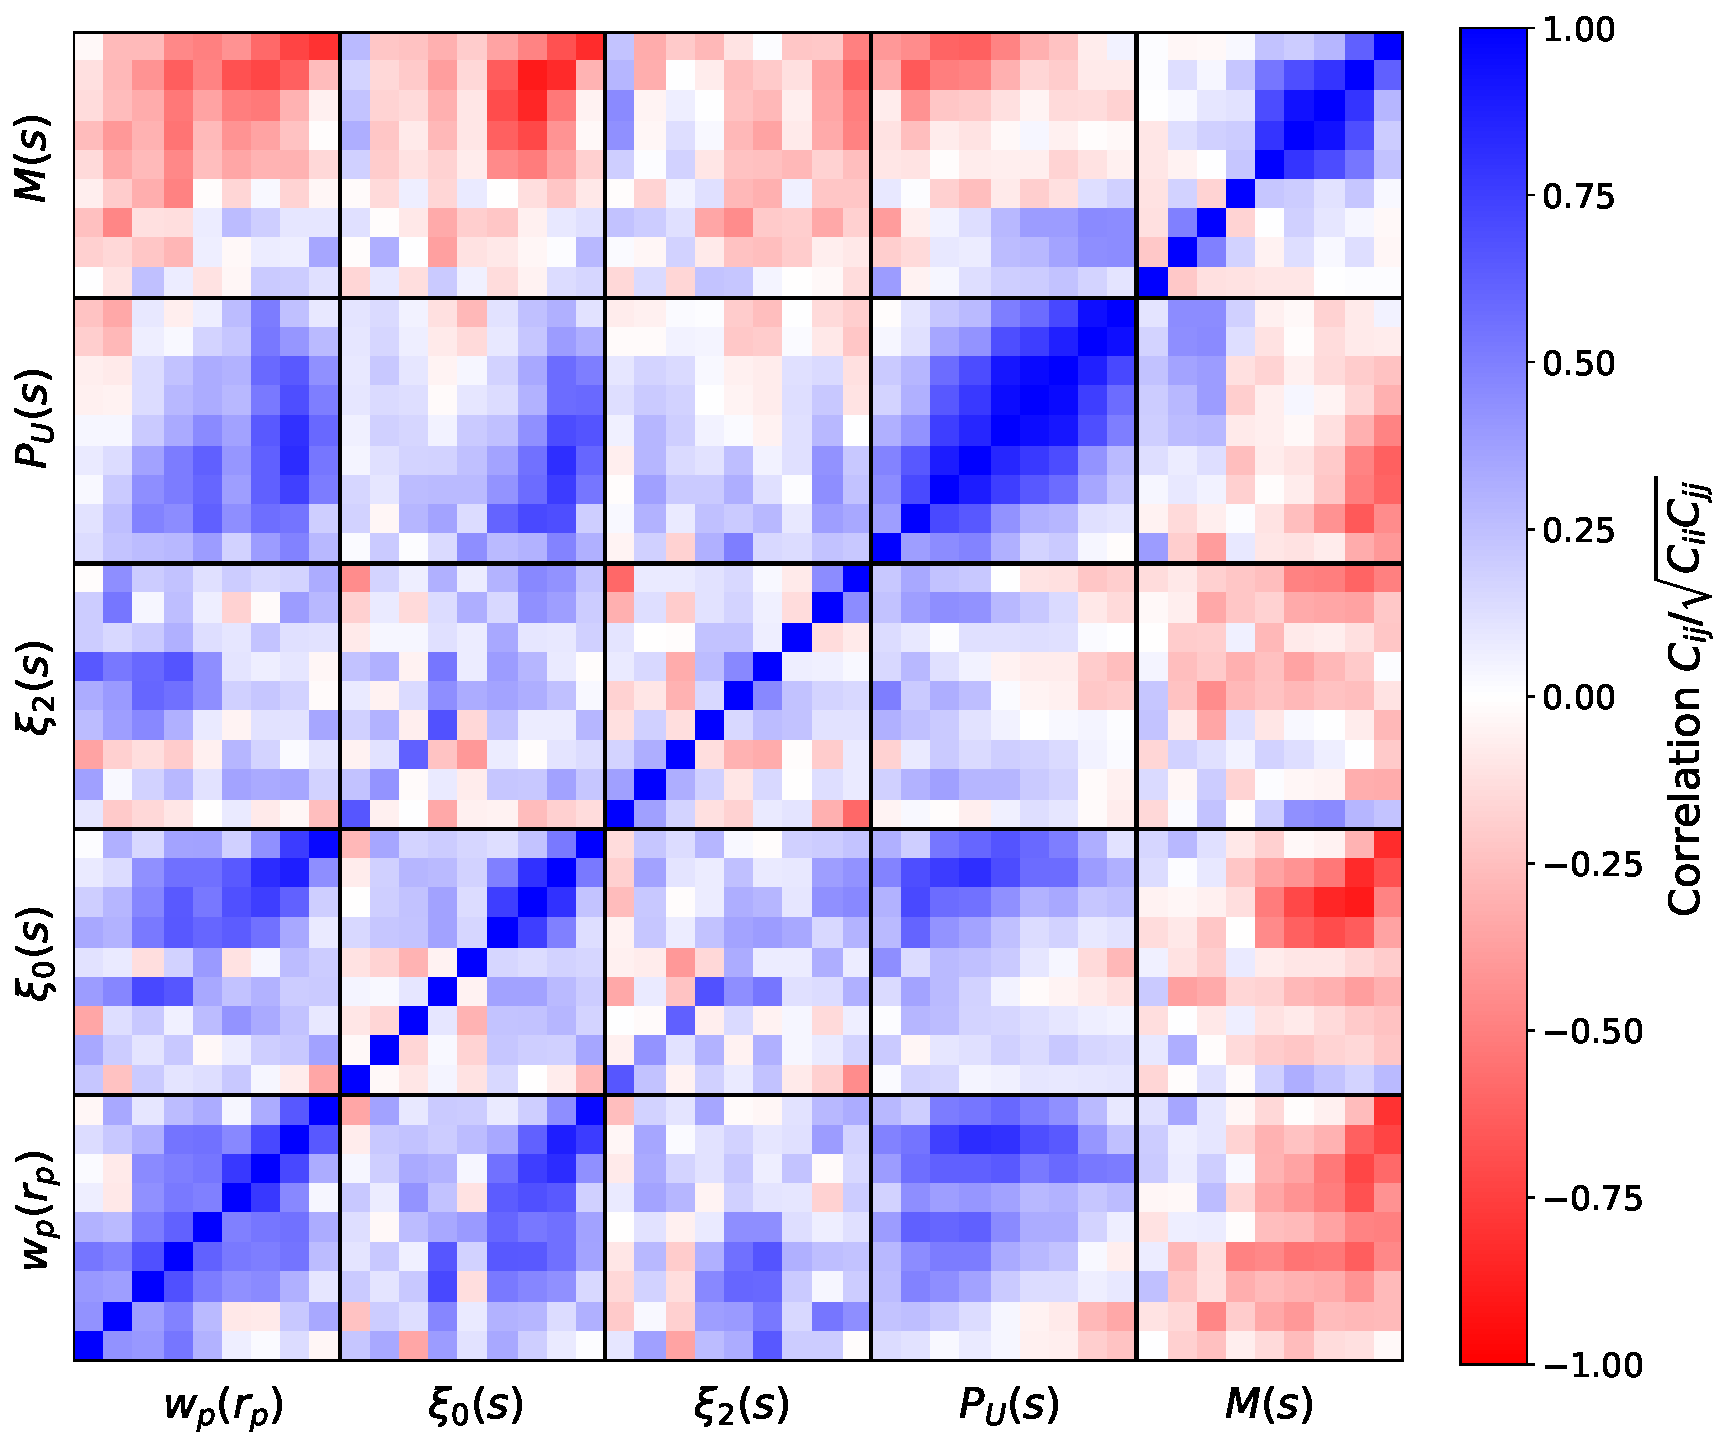
\includegraphics[width=0.33\textwidth]{corr_aemulus}}
\subfloat[\label{fig:cov_emuperf}] {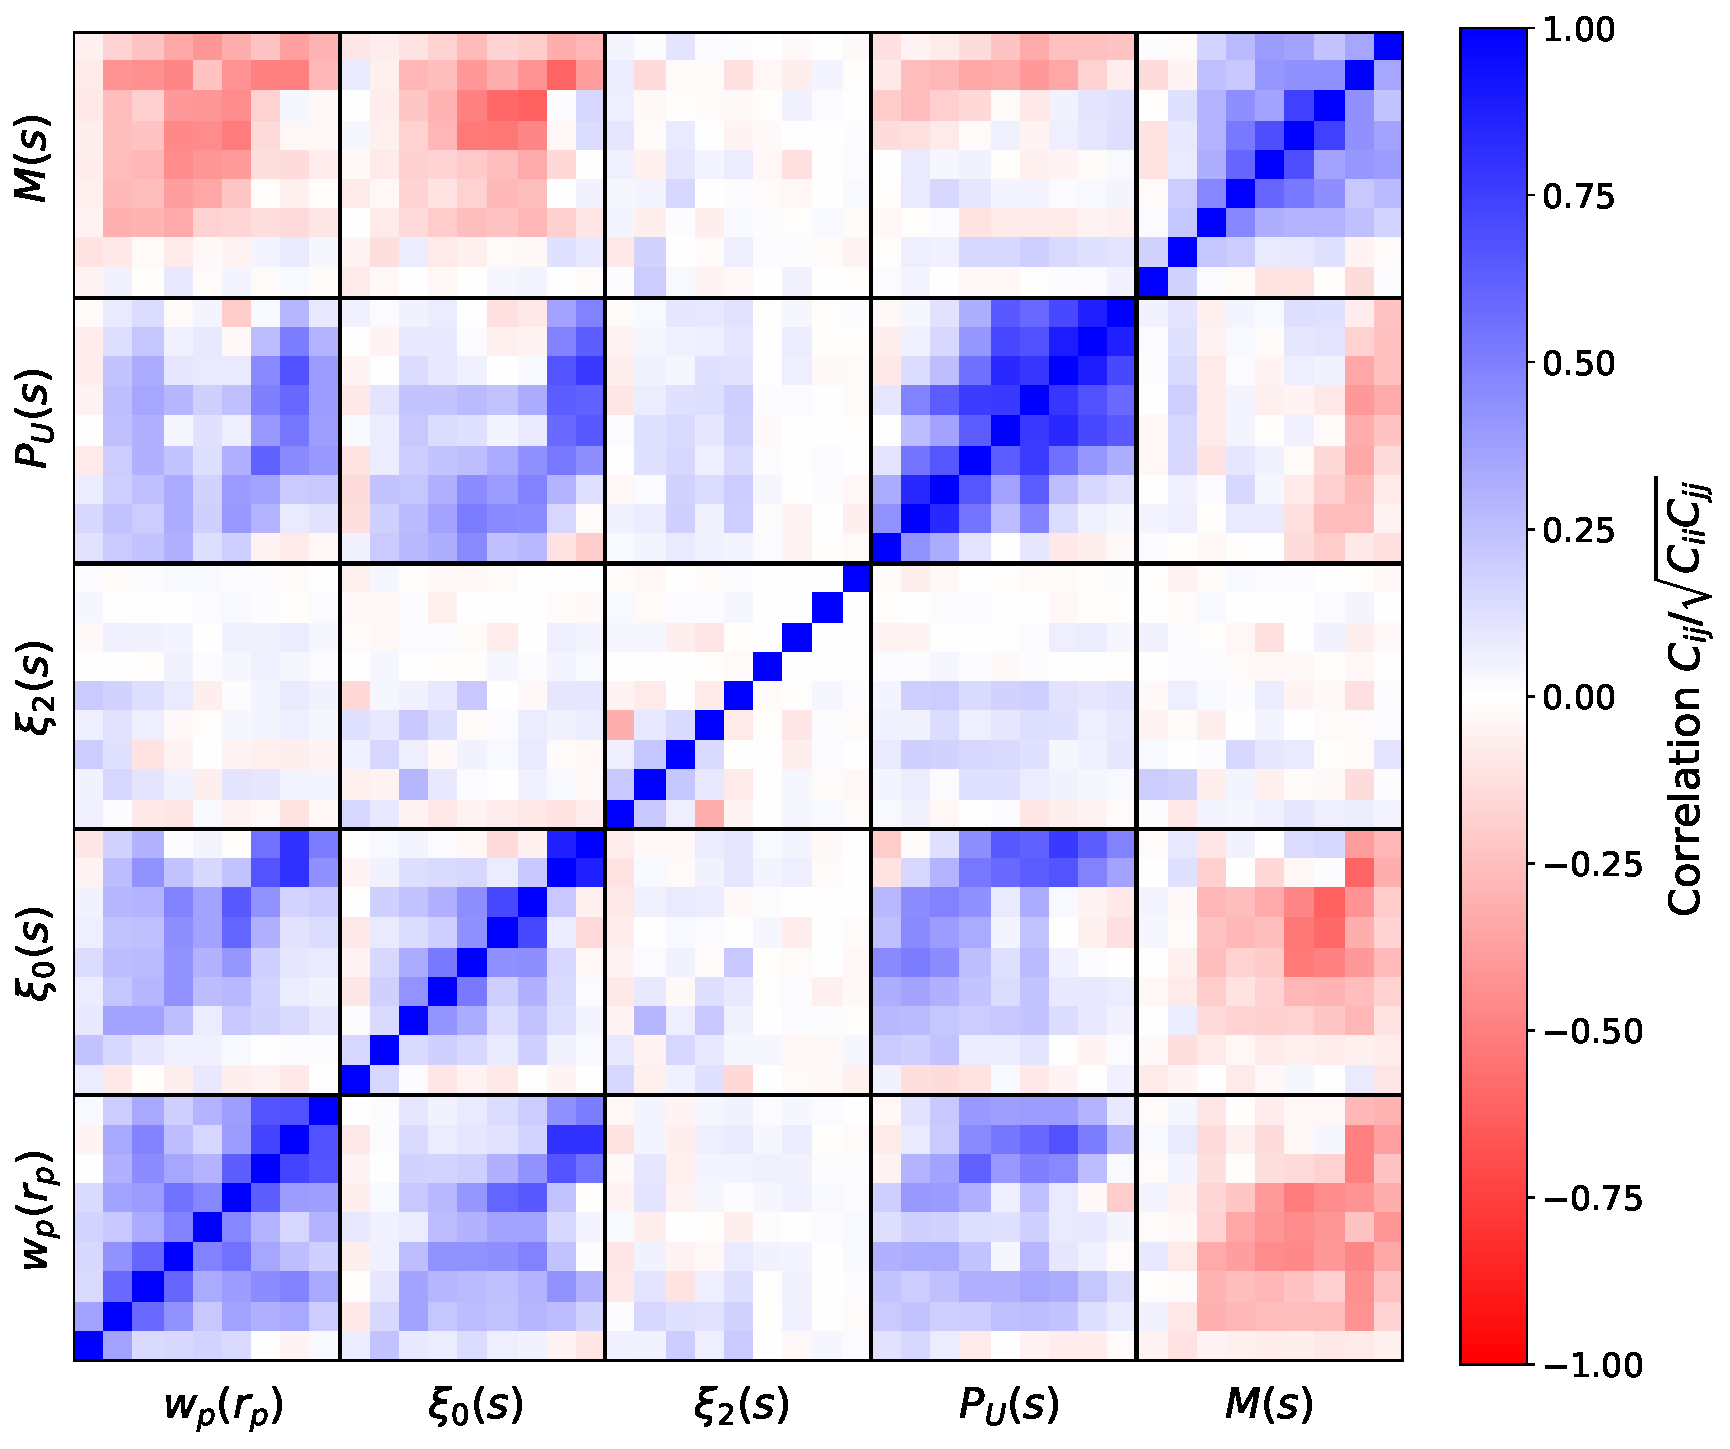
\includegraphics[width=0.33\textwidth]{corr_emuperf}}
\subfloat[\label{fig:cov_smooth_emuperf}]{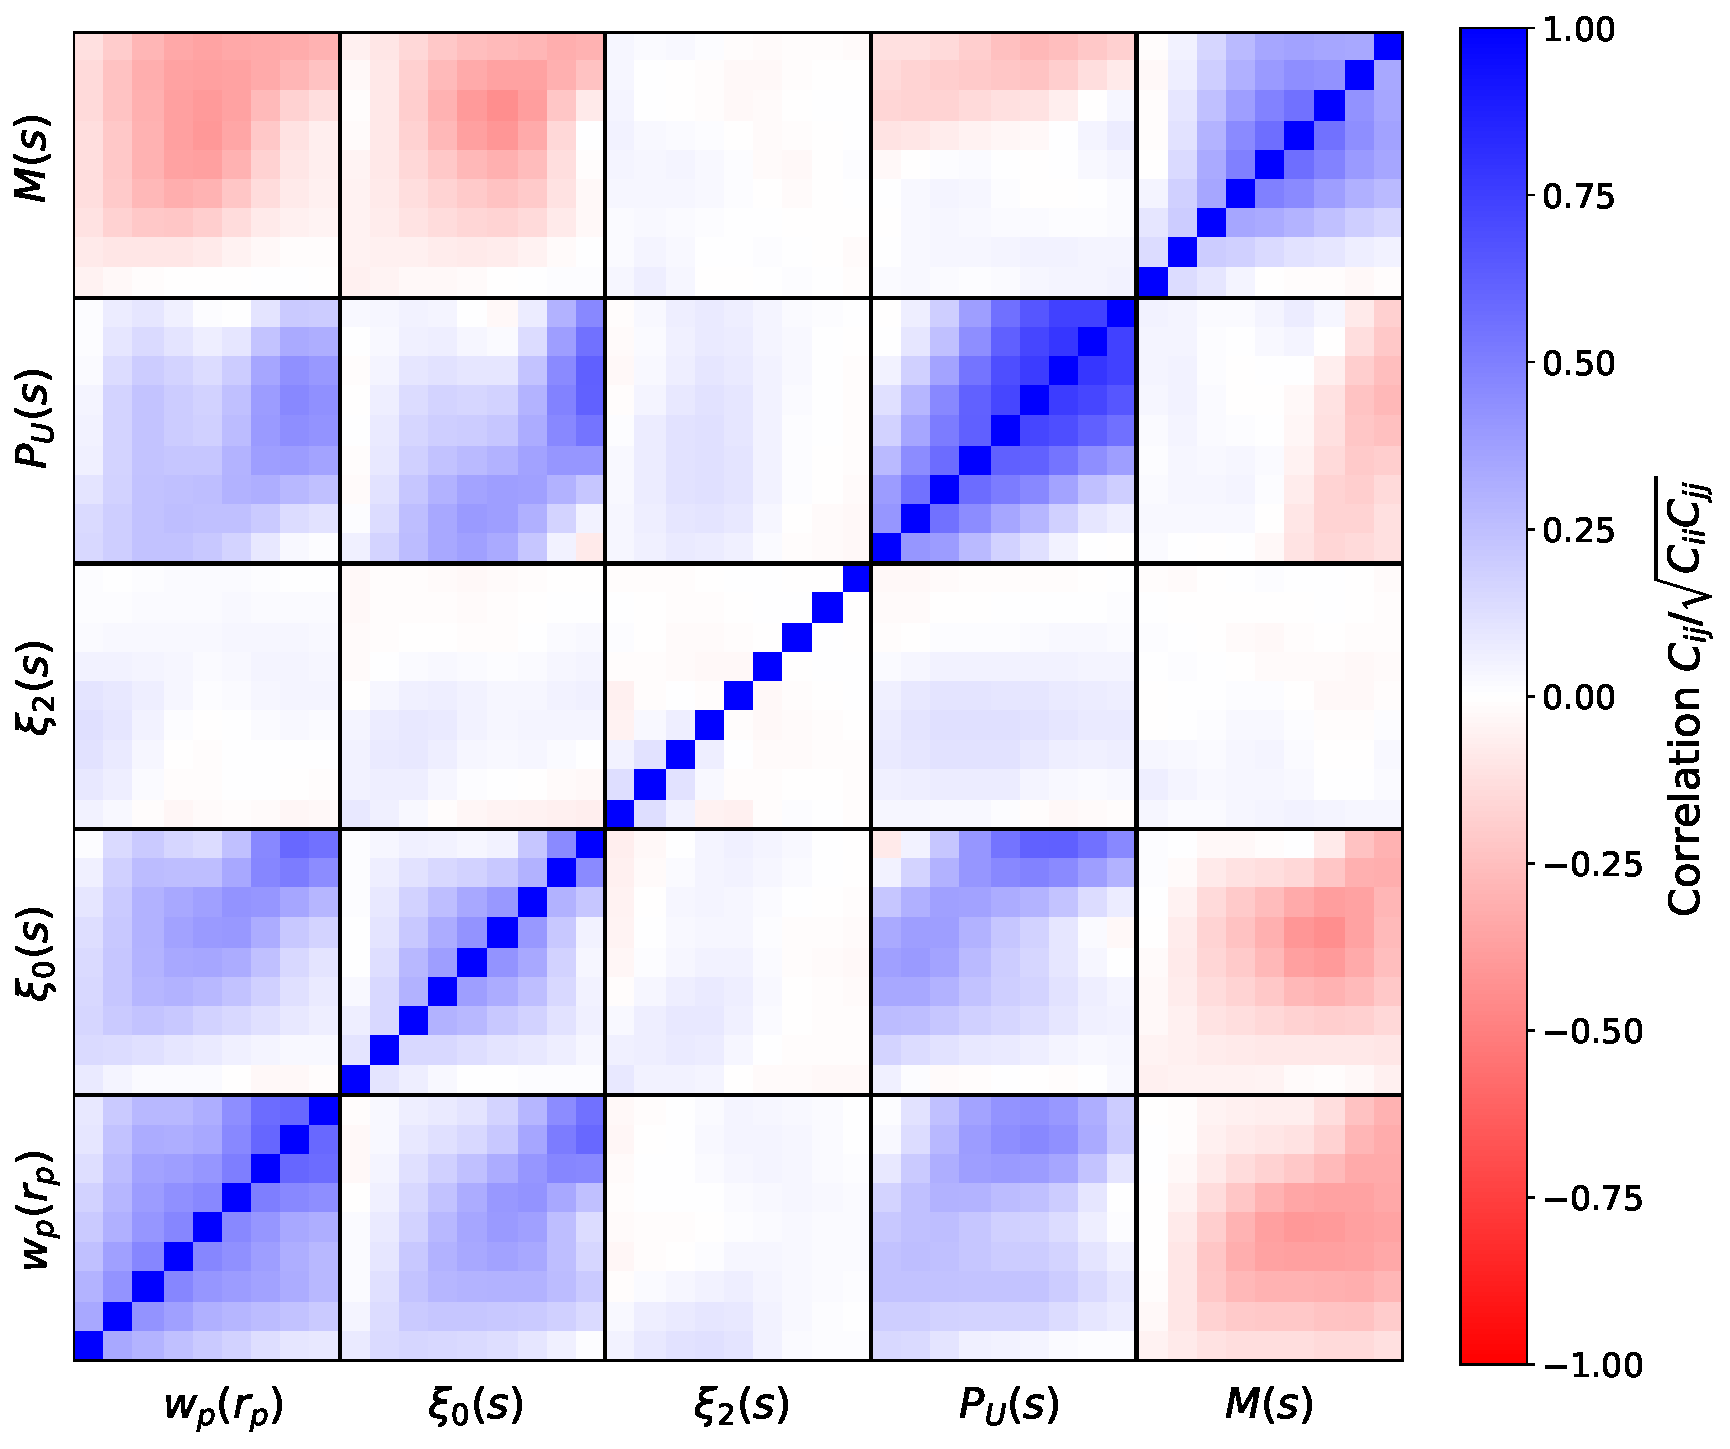
\includegraphics[width=0.33\textwidth]{corr_smoothgauss_emuperf}}
\caption{Correlation matrices for visualizing the covariance matrices used in the analysis, for all five observables. The panels show correlation matrices constructed from (a) the \aemulus sample covariance $\cov{aemulus}$, (b) the emulator performance covariance $\cov{perf}$, and (c) the performance covariance with a Gaussian smoothing $\cov{perf,smooth}$. The color bar shows the correlation quantity $C_{ij}/\sqrt{C_{ii}C_{jj}}$, where $C_{ij}$ are elements of the correlation matrix.}
\label{fig:covs}
\end{figure*}

To perform inference using our emulator, we require a covariance matrix describing the correlations between the observables, as well as between the bins of a single observable.
This covariance includes both the uncertainties introduced by the emulator, contained in $\cov{emu}$, and the sample variance of the data on which we are performing parameter recovery, $\cov{data}$.
We combine these into the total covariance $\covtot$ that we will use in our likelihood function (see \S\ref{sec:inference}),
\begin{equation}
    \covtot = \cov{emu} + \cov{data}.
\end{equation}

We define the overall emulator performance covariance $\cov{perf}$ as the combination of both the intrinsic emulator prediction error ($\cov{emu}$) and the covariance of the data on which the emulator is tested, $\cov{test}$, so to obtain $\cov{emu}$ we must subtract off $\cov{test}$:
\begin{equation}
     \cov{emu} = \cov{perf} - \cov{test}.
\end{equation}
We obtain $\cov{perf}$ by computing the covariance of the fractional error between the emulator predictions and the measurements on the data (and then smoothing this matrix to handle noise from our limited number of simulations, as described below).
The performance covariance on our test set with $N_\mathrm{test}=3500$ observations indexed by $n$ is then:
\begin{eqnarray}
    \label{eq:frac_pred}
    \cov{perf} &=& \frac{1}{N_\mathrm{test}-1} \sum_n^{N_\mathrm{test}} \bm{f}_n \cdot \bm{f}_n\T ~, \\
    \bm{f}_n &=& \frac{ \bm{y}_{n,\mathrm{pred}} - \bm{y}_{n,\mathrm{test}} }{ \bm{y}_{n,\mathrm{test}} },
\end{eqnarray}
where $\bm{y}$ is a vector of the measured observables (which can be a concatenation of multiple observable vectors).
Note that we know the expectation value of these fractional errors should be zero, so we assume $\bar{\bm{f}}_{n}=0$ when computing the covariance.
The computed $\cov{perf}$ is visualized in Figure~\ref{fig:cov_emuperf}, for all 5 observables.

We compute $\cov{test}$ using the \aemulus test set, which has $N_\mathrm{cosmos}=7$ different cosmologies $c$, and $N_\mathrm{box}=5$ boxes (realizations) $b$ for each cosmology. 
These are each populated with $H=100$ HOD models $h$. 
We utilize the fact that we have multiple boxes per cosmology to estimate the sample variance.
We choose a single HOD model in the middle of the parameter space, and for each cosmology populated with this HOD, we compute the mean value of the observable $\bar{\bm{y}}_{c}$ of the $N_\mathrm{box}$ boxes,
\begin{equation}
    \bar{\bm{y}}_{c} = \frac{1}{N_\mathrm{box}} \sum_b^{N_\mathrm{box}} {\bm{y}_{b,c}} .
\end{equation}
We compute the fractional deviation from this mean $\bm{d}_{b,c}$ for each of box of a given cosmology,
\begin{equation}
    \bm{d}_{b,c} = \frac{ {\bm{y}_{b,c} - \bar{\bm{y}}_{c}} } {\bar{\bm{y}}_{c}} .
\end{equation}
We finally compute the covariance of these deviations from the mean,
\begin{equation}
    \cov{aemulus} = \frac{1}{N_\mathrm{box}N_\mathrm{cosmos}-1} \sum_{b}^{N_\mathrm{box}} \sum_{c}^C \bm{d}_{b,c} \cdot \bm{d}_{b,c}\T ~.
\end{equation}
The computed $\cov{aemulus}$ is shown in Figure~\ref{fig:cov_aemulus}.

When we compute Equation~\eqref{eq:frac_pred} used in $\cov{perf}$, the observable values $\bm{y}_{n,\mathrm{test}}$ we use are the mean observable over the $N_\mathrm{box}$ test boxes for each cosmology.
This essentially increases the volume of the test set by a factor of $N_\mathrm{box}$, and uncertainty scales inverse proportionally to volume \citep{KlypinPrada2018}.
Thus in order to combine $\cov{perf}$ and $\cov{test}$, we need to scale the latter to match the effective volume of the former,
\begin{equation}
    \cov{test} = \frac{1}{N_\mathrm{box}} \, \cov{aemulus} .
\end{equation}

We can now use $\cov{test}$ to construct $\cov{emu}$, and combine it with $\cov{data}$ to obtain the total covariance.
For our tests, we are performing parameter recovery on the \aemulus\ test simulations themselves, so we have $\cov{data} = \cov{test}$, and we get simply $\covtot = \cov{perf}$.
In future applications to real data, we will need to include both $\cov{data}$ and $\cov{test}$ in the covariance matrix construction.

We do use the \aemulus covariance $\cov{test}$ as input to the Gaussian process emulator.
The GP requires an estimation of the uncertainty on the training set.
As the training and test sets are from the same simulation suite, but the test set contains multiple realizations of the same cosmology, we use the test set to estimate the training set uncertainty.
We use the diagonal elements of $\cov{test}$ as the variances $\sigma_n^2$ in Equation~\eqref{eq:gp_pred}.

We perform a smoothing on the total covariance matrix, here $\cov{perf}$, to avoid inference issues caused by the initially noisy matrix.
Our procedure follows that of \cite{Lange2022}, and has been shown by \cite{Mandelbaum2013} to give essentially the same results as applying the Hartlap correction to unbias the inverse covariance matrix \citep{Hartlap2007}.
We first compute the correlation matrices, with elements given by $C_{ij}/\sqrt{C_{ii}C_{jj}}$, where $C_{ij}$ are the elements of the covariance matrix.
The diagonal elements of the correlation matrix must be equal to 1, as each element is perfectly correlated with itself, and the surrounding elements are typically much smaller, so we start by replacing the diagonal elements with the mean of its four neighbors.
We then apply a basic Gaussian kernel with width one, to smooth the matrix.
Finally we replace back the diagonal elements.
The smoothed total covariance matrix, $\cov{perf,smooth}$, is shown in Figure~\ref{fig:cov_smooth_emuperf}.
A comparison between using the smoothed and original covariance matrices for parameter inference is shown in Appendix~\ref{appendix:cov}.


\subsection{Inference with Emulator+MCMC}
\label{sec:inference}

We use Markov Chain Monte Carlo (MCMC) to infer the parameters of the mock catalog given the measured statistics, using the trained Gaussian process emulator to predict the statistic at each set of parameters.
For the MCMC process, we use the package \texttt{dynesty} \citep{Speagle2020}, which implements dynamic nested sampling.
Nested sampling is a method for both obtaining posterior values from a likelihood function and estimating the Bayesian evidence \citep{Skilling2006}; dynamic nested sampling improves upon this by varying the number of live points used in the computation \citep{Higson2019}.
While we don't directly make use of the evidence in this work, dynamic nested sampling is faster and more robust than other standard MCMC approaches.

For the HOD and assembly bias parameters, as well as $\gf$, we use a uniform prior with a range given in Table 3 of \cite{Zhai2022}, with an additional constraint on $\msat$ to be above $10^{11.5} \: M_\odot$.
For the cosmological parameters, we use a multi-dimensional Gaussian prior defined by the mean and covariance of the cosmology training set parameter space (see Figure 3 in \cite{DeRose2018}).
We also try a flat prior and a high-dimensional ellipsoid, and find no change in the results; we choose to use the multi-dimensional Gaussian to improve stability and speed of the MCMC runs.

We use a likelihood $\like$ of
\begin{equation}
    \mathrm{ln} \, \like = -\frac{1}{2} \bigg( \frac{\bm{y}_\mathrm{pred} - \bm{y}_\mathrm{test}}{\bm{y}_\mathrm{test}} \bigg)\T \covtot\inv \bigg( \frac{\bm{y}_\mathrm{pred} - \bm{y}_\mathrm{test}}{\bm{y}_\mathrm{test}} \bigg)
\end{equation}
where $\covtot$ is the covariance matrix described in \S\ref{sec:cov}, and $\bm{y}$ is a vector containing the concatenated observables.
Here $\bm{y}_\mathrm{test}$ is the statistics measured directly on the test set mock catalog on which we are performing parameter recovery, averaged over the $N_\mathrm{box} = 5$ boxes per cosmology and HOD model, and $\bm{y}_\mathrm{pred}$ is the emulator prediction for the observables at the given point in parameter space. 


\section{Results}
\label{sec:results_aemulus}

We present the results of our emulation and inference on the \aemulus test suite.
We show the emulator performance (\S\ref{sec:emuperf}), the results of recovery tests on a single test model (\S\ref{sec:recovery_single}) and a larger test sample (\S\ref{sec:recovery_statistical}), and an analysis of the scale dependence of our results (\S\ref{sec:scaledep}).

\subsection{Emulator performance}
\label{sec:emuperf}

\begin{figure*}[htp!]
\centering
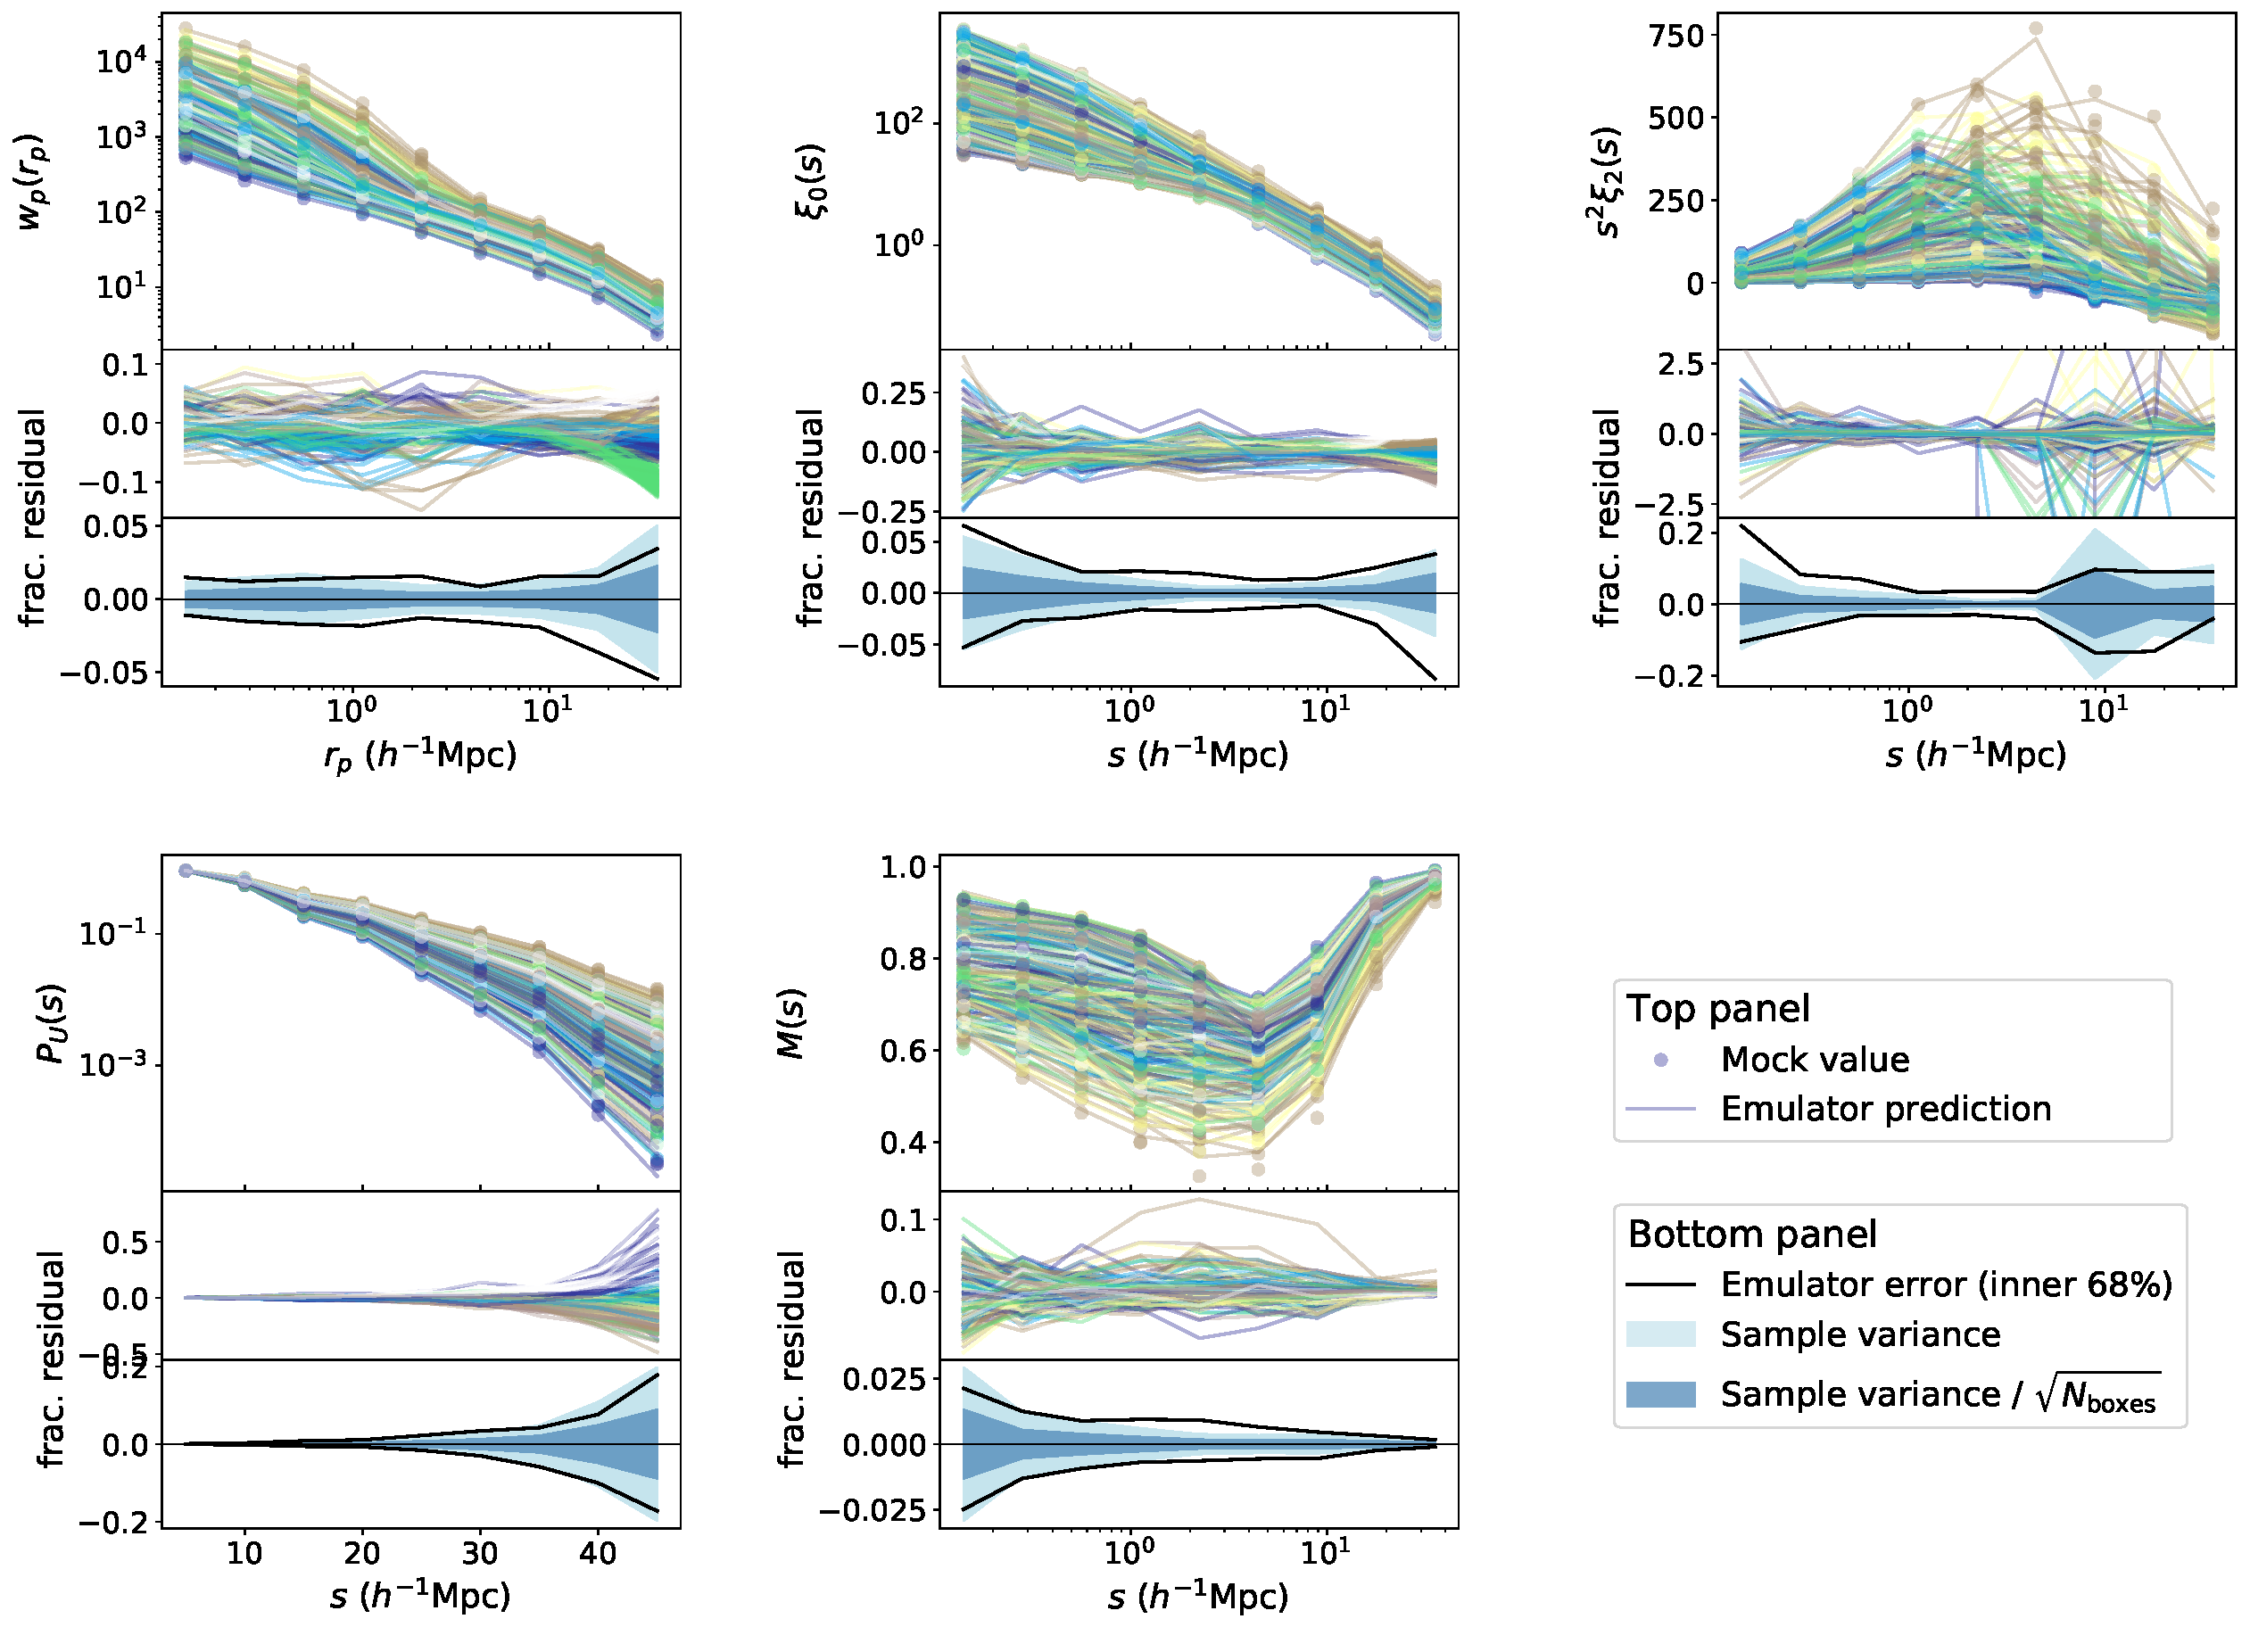
\includegraphics[width=0.9\textwidth]{emu_accuracy}
\caption{The accuracy of our Gaussian process emulator predictions for the projected correlation function $w_{\rm p}(r_{\rm p})$, monopole and quadrupole of the two-point correlation function $\xi_o(s)$ and $\xi_2(s)$, underdensity probability function $P_U(s)$, and marked correlation function $M(s)$. Top panels show the  measured statistics (circles), averaged over $N_\mathrm{box}$ test boxes for each model, and the corresponding emulator predictions (lines) for each cosmology+HOD model. The colors denote different cosmologies. The middle panels show the fractional error of each of the predictions. The bottom panels show the inner 68\% region of the fractional errors (black line), compared to the sample variance of the simulations (light blue). The sample variance scaled by $\sqrt{N_\mathrm{box}}$ adjusts for the effective increase in volume of comparing emulator predictions to the mean of $N_\mathrm{box}$ measurements.}
\label{fig:emu_accuracy}
\end{figure*}

The performance of the emulators is shown in Figure~\ref{fig:emu_accuracy}, for each of the observables for all 700 test models.
For each test cosmology, we compute the statistic for each of the $N_\mathrm{box}=5$ realizations, and take the measured statistic to be the mean of these.
We compute the fractional error between the predicted and measured statistic, and define the error as the symmetrized inner 68\% error.
We compare this error to the sample variance, the square root of the diagonal of $\cov{aemulus}$ for the given observable, as well as this uncertainty scaled by $\sqrt{N_\mathrm{box}}$.
This scaled uncertainty takes into account the increased precision provided by comparing to the mean over multiple boxes; the covariance matrix scales as the inverse volume, as explained in \S\ref{sec:cov}, and averaging over multiple boxes effectively increases the volume, so we obtain this factor of $\sqrt{N_\mathrm{box}}$ (the result is equivalent to taking the square root of the diagonal of $\cov{test}$).

Our emulators achieve very good accuracy across most observables and scales.
For $\wprp$, we obtain $\simo2\%$ error on scales up to 10 $\hMpc$, and $2$--$5\%$ error up to 50 $\hMpc$.
For $\cfm$, we achieve $\simo2\%$ error on scales between $1$--$10 \, \hMpc$, and up to $5\%$ outside that range.
$\cfq$ has the lowest performance because of high noise levels, with $\simo5\%$ error from $1$--$5 \, \hMpc$ and $10$--$20\%$ error at other scales.
For $\upf$, we see extremely small errors of $<0.5\%$ below $20 \, \hMpc$ scales, as a result of the low variation of the statistic there; up to $35 \, \hMpc$, we still achieve $\simo5\%$ error.
Finally for $\mcf$, we achieve $1$--$2.5\%$ error on scales up to 10 $\hMpc$, and $<1\%$ error at larger scales.

At most scales, we see that our emulator error is comparable to the raw sample variance of the \aemulus simulations.
Comparing to the sample variance adjusted for the effective volume, we see that the emulator prediction error is somewhat greater than this quantity; this is expected, as the emulation performance error includes both the sample variance and the emulator prediction error.


\subsection{Parameter inference recovery tests on single mock}
\label{sec:recovery_single}

We apply our approach with our GP emulator and MCMC to obtain the posterior distributions of the 18 parameters for a given cosmology+HOD model.
As we have 5 realizations of each test cosmology, we populate all of these with the same HOD and measure the desired statistics on each of them, and then take the mean of these to obtain the measured statistic. 
These are the values that we compare to the emulator prediction at each step of the MCMC chain.
The \aemulus test volume summed over the 5 boxes is $N_\mathrm{box} \times \, (1.05 \hGpc)^3 = 5.79 \, (\hGpc)^3$.
This is significantly larger than the volume of the highest-redshift shell used in \aemulus V: $1.63 \, (\hGpc)^3$, based on the redshift range $0.48 < z < 0.62$ and the CMASS+LOWZ area of 8447 deg$^2$.
For that analysis, the CMASS data was subsampled to a number density of $2 \times 10^{-4} (\hMpc)^{-3}$, the same as used here, and thus we can make a direct comparison of the volumes. 
The larger volume of the \aemulus test boxes by a factor of a few suggests that these are a meaningful test of the precision we will achieve when we apply the approach to data.

\begin{figure*}%[htp!]
\centering
\subfloat[\label{fig:contour_single_cosmo}]{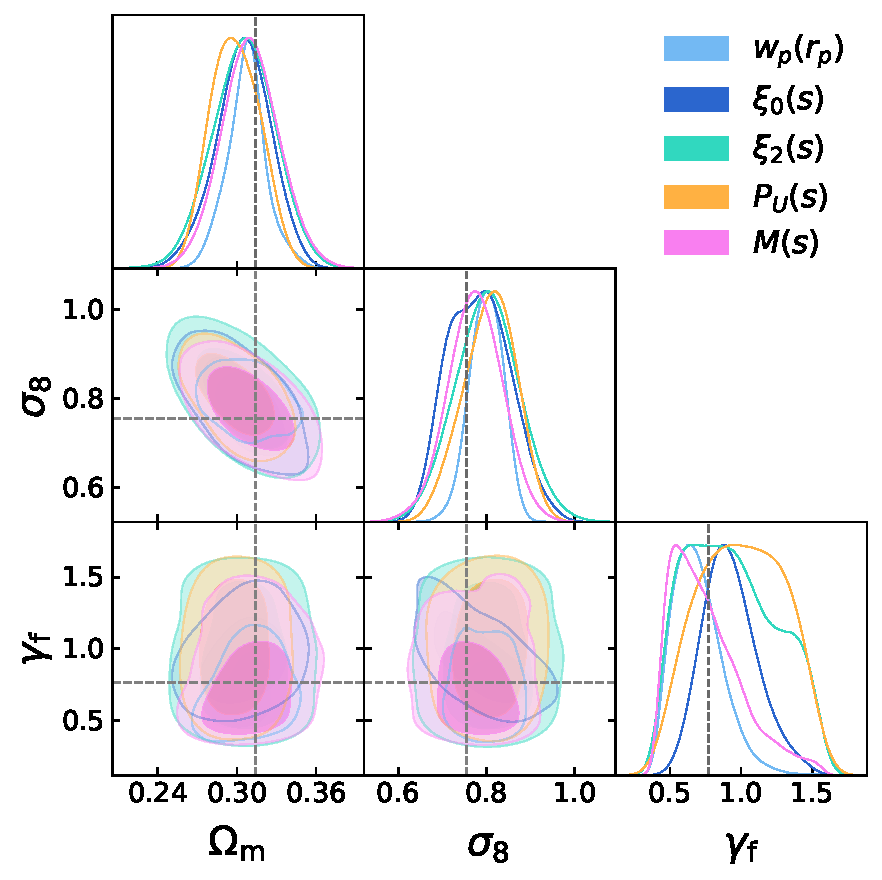
\includegraphics[width=0.4\textwidth]{contour_single_cosmo}}
\hspace{0.07\textwidth}
\subfloat[\label{fig:contour_single_hodab}] {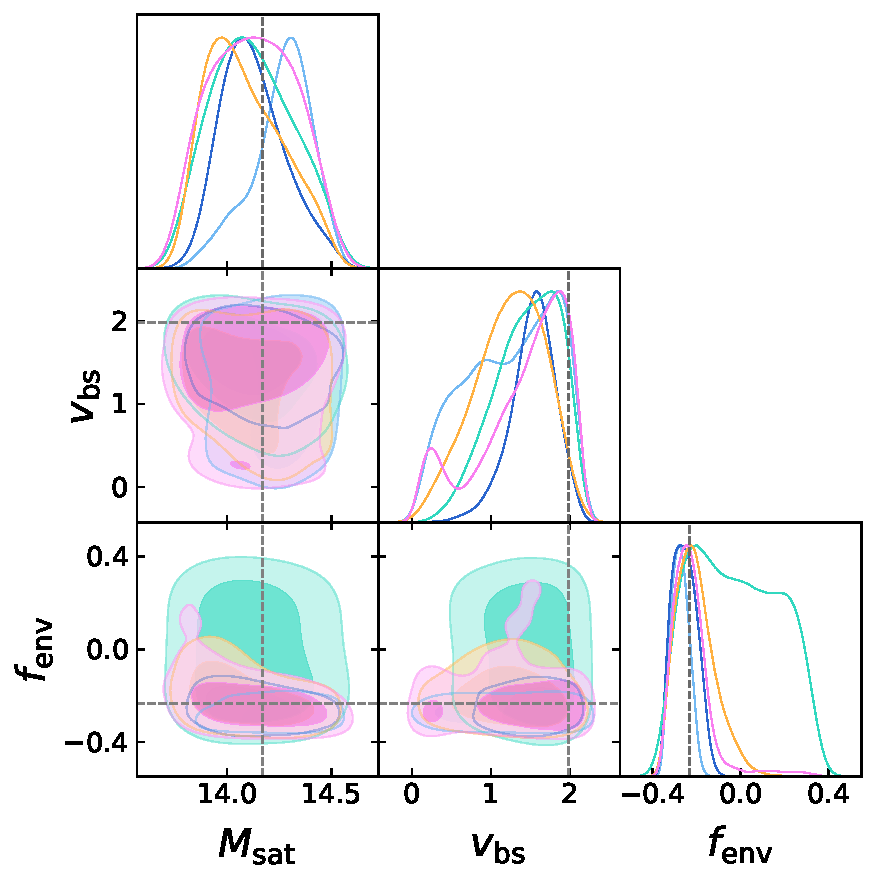
\includegraphics[width=0.4\textwidth]{contour_single_hodab}}
\caption{Recovery tests for a single cosmology+HOD model, using a single observable for each MCMC chain. Contours are shown for (a) key cosmological parameters and (b) key HOD and assembly bias parameters.}
\label{fig:contours_single}
\end{figure*}

We start by performing the inference based on each of the five observables alone. 
In Figure~\ref{fig:contours_single}, we show the results on a single cosmology+HOD model; Figure~\ref{fig:contour_single_cosmo} shows key cosmological parameters, and Figure~\ref{fig:contour_single_hodab} shows key HOD and assembly bias parameters.
We have chosen the latter set of parameters as they are particularly degenerate with cosmological parameters.
We see that the different observables have varying effectiveness at constraining the parameters. 
For instance, $\wprp$ and $\mcf$ provide strong constraints on their own on the cosmological parameters, while $\cfq$ and $\upf$ constrain them more weakly, in particular in the case of $\gamma_f$. 
For the HOD and assembly bias parameters, $\wprp$ provides a slightly tighter constraint on $\msat$ than the other observables, $\cfm$ constrains $\vbs$ well on own, and $\cfq$ provides little constraining power on $\fenv$; otherwise, all the observables constrain these parameters to a similar precision.
Note that this is just a single test model, but is somewhat representative of overall trends.

\begin{figure*}
\centering
\subfloat[\label{fig:contour_addin_cosmo}]{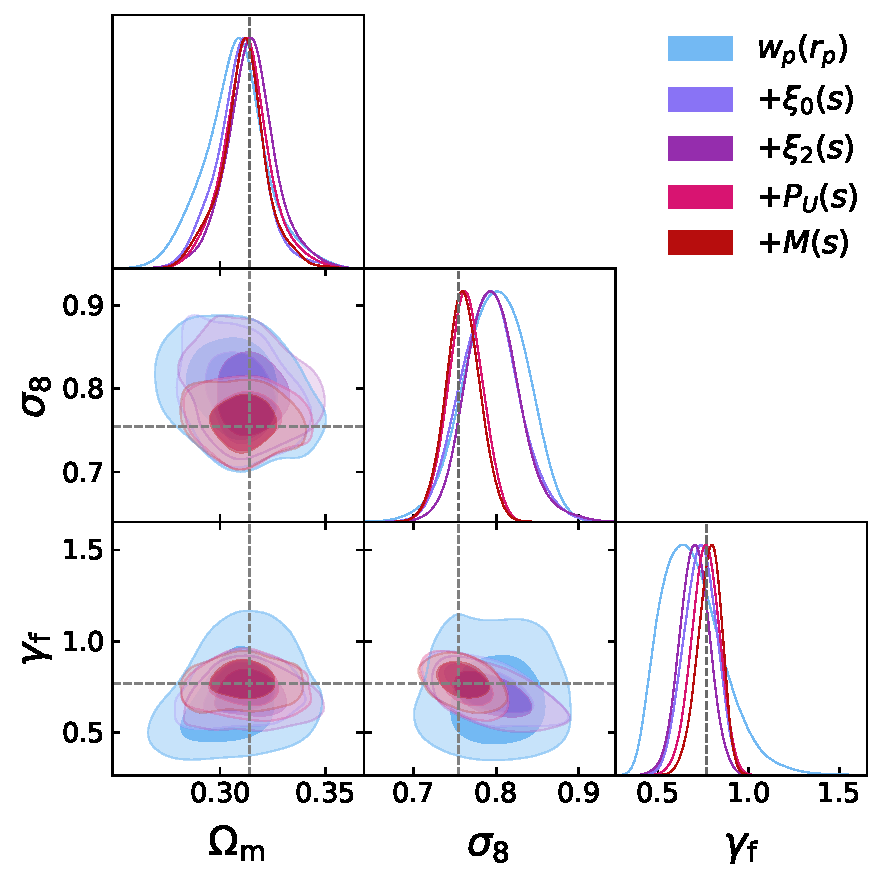
\includegraphics[width=0.4\textwidth]{contour_addin_cosmo}}
\hspace{0.07\textwidth}
\subfloat[\label{fig:contour_addin_hodab}] {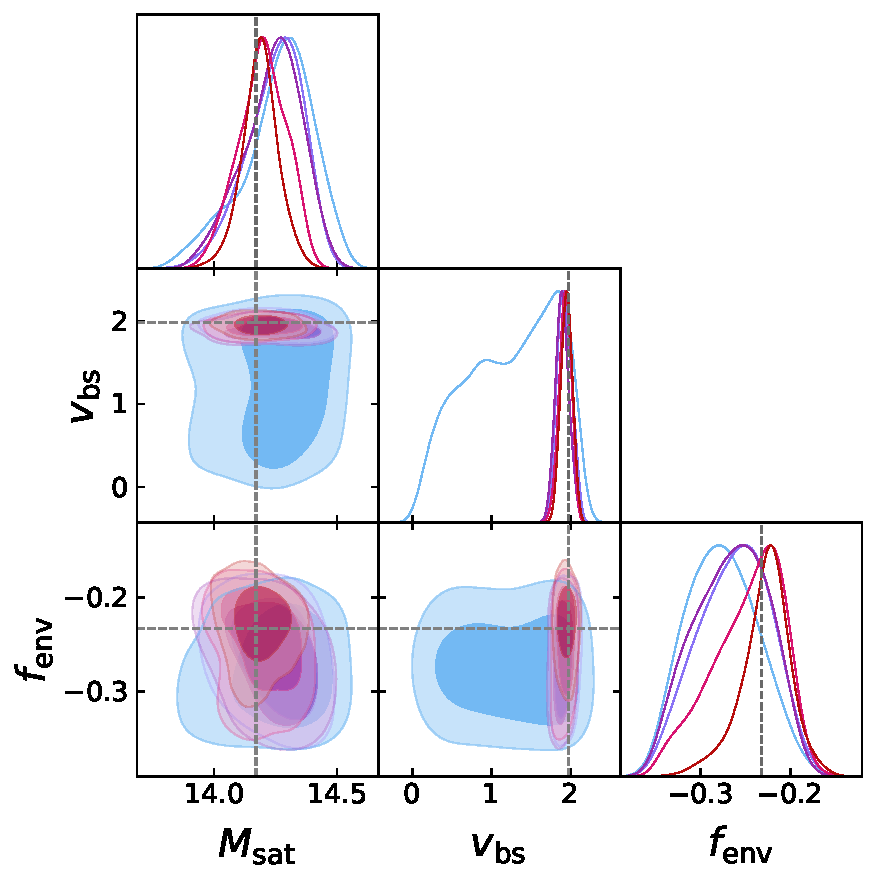
\includegraphics[width=0.4\textwidth]{contour_addin_hodab}}
\caption{Recovery tests for a single cosmology+HOD model, successively adding in the observables. Contours are shown for (a) key cosmological parameters and (b) key HOD and assembly bias parameters.}
\label{fig:contours_addin}
\end{figure*}

Next, we explore the constraining power of combining the observables when running the MCMC chains.
We start with just $\wprp$, and then one at a time add in $\cfm$, $\cfq$, $\upf$, and $\mcf$.
The results are shown in in Figure~\ref{fig:contours_addin} for the same model and parameters as Figure~\ref{fig:contours_single}.
As additional observables are added, we obtain tighter and tighter constraints on the parameters.
In particular, we can compare the constraints with the three standard observables to those when including the two beyond-standard statistics.
For the parameters $\sigma_8$, $M_\mathrm{sat}$, $\fenv$, and $\delta_\mathrm{env}$, we see a sharp increase in precision and accuracy when including these new statistics. 
The other parameters show a smaller but still significant increase.
This is promising for the power of the beyond-standard statistics to add additional cosmological information beyond that provided by typical statistics.

\begin{figure*}%[htp!]
\centering
\subfloat[\label{fig:recovery_single}]{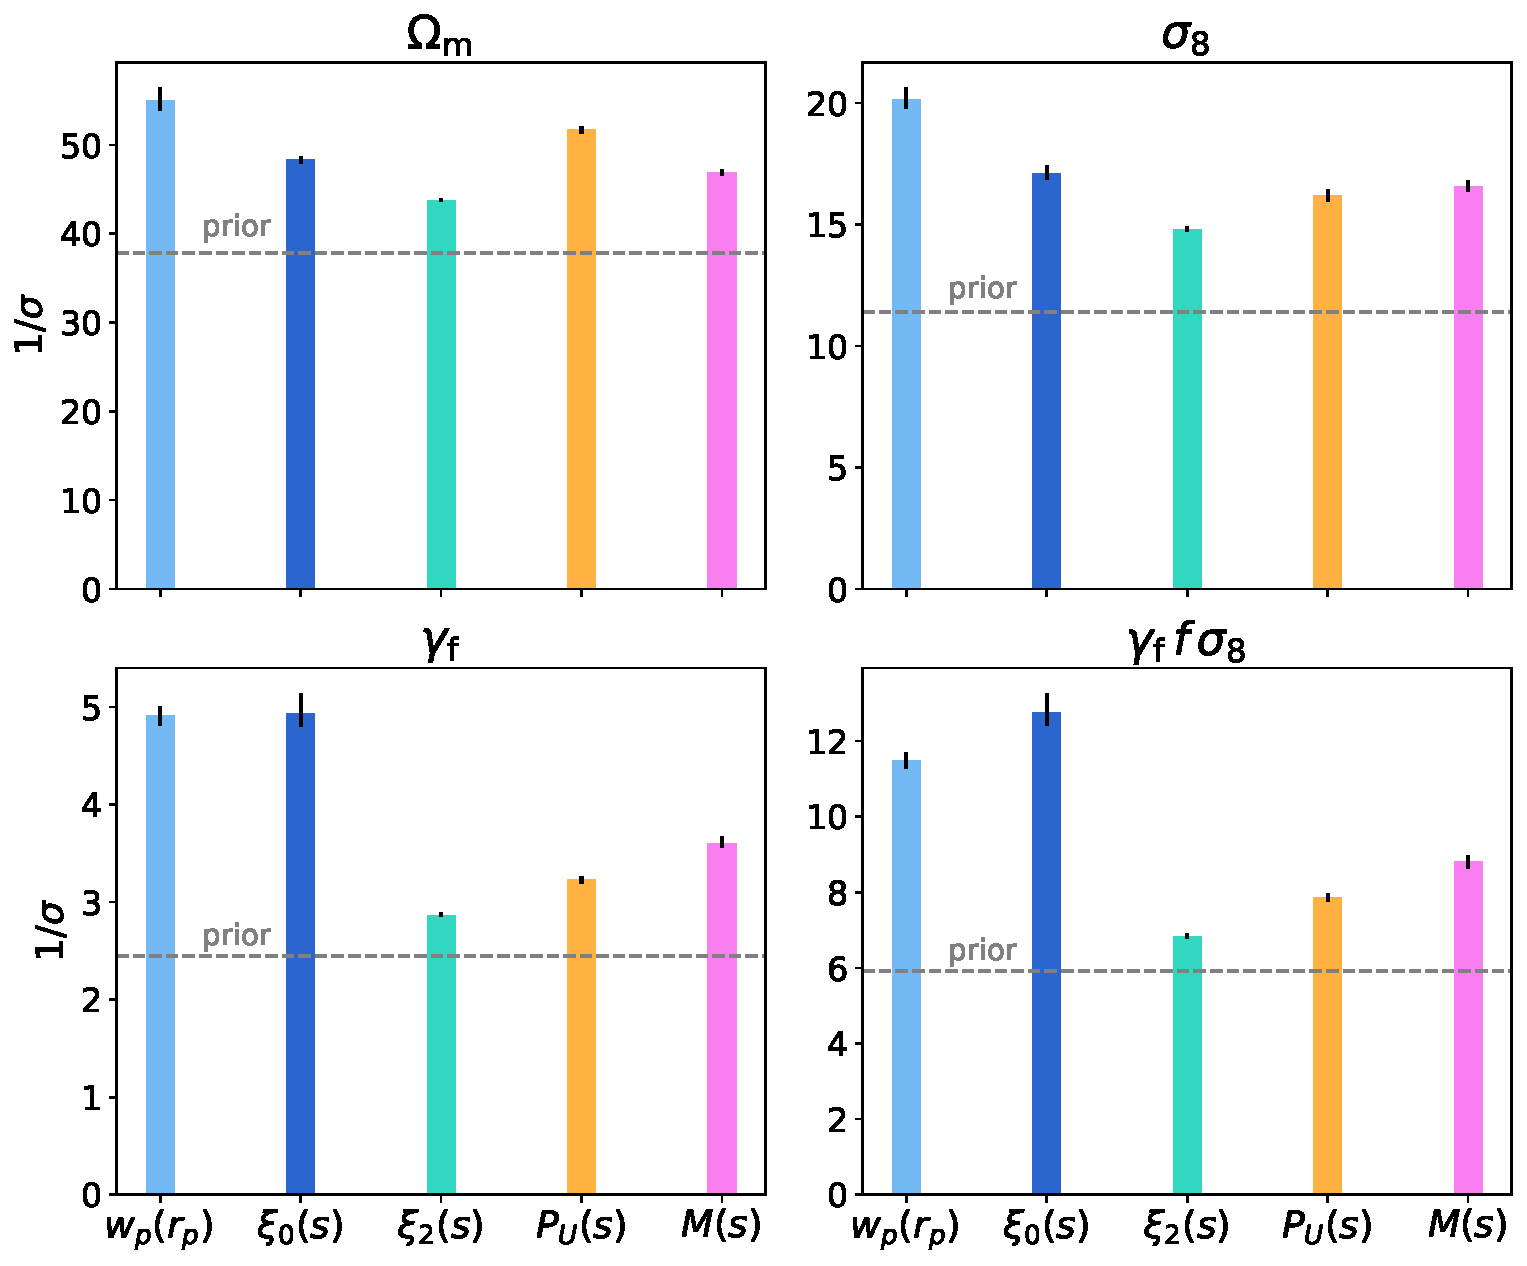
\includegraphics[width=0.465\textwidth]{recovery_single}}
\hspace{0.04\textwidth}
\subfloat[\label{fig:recovery_addin}] {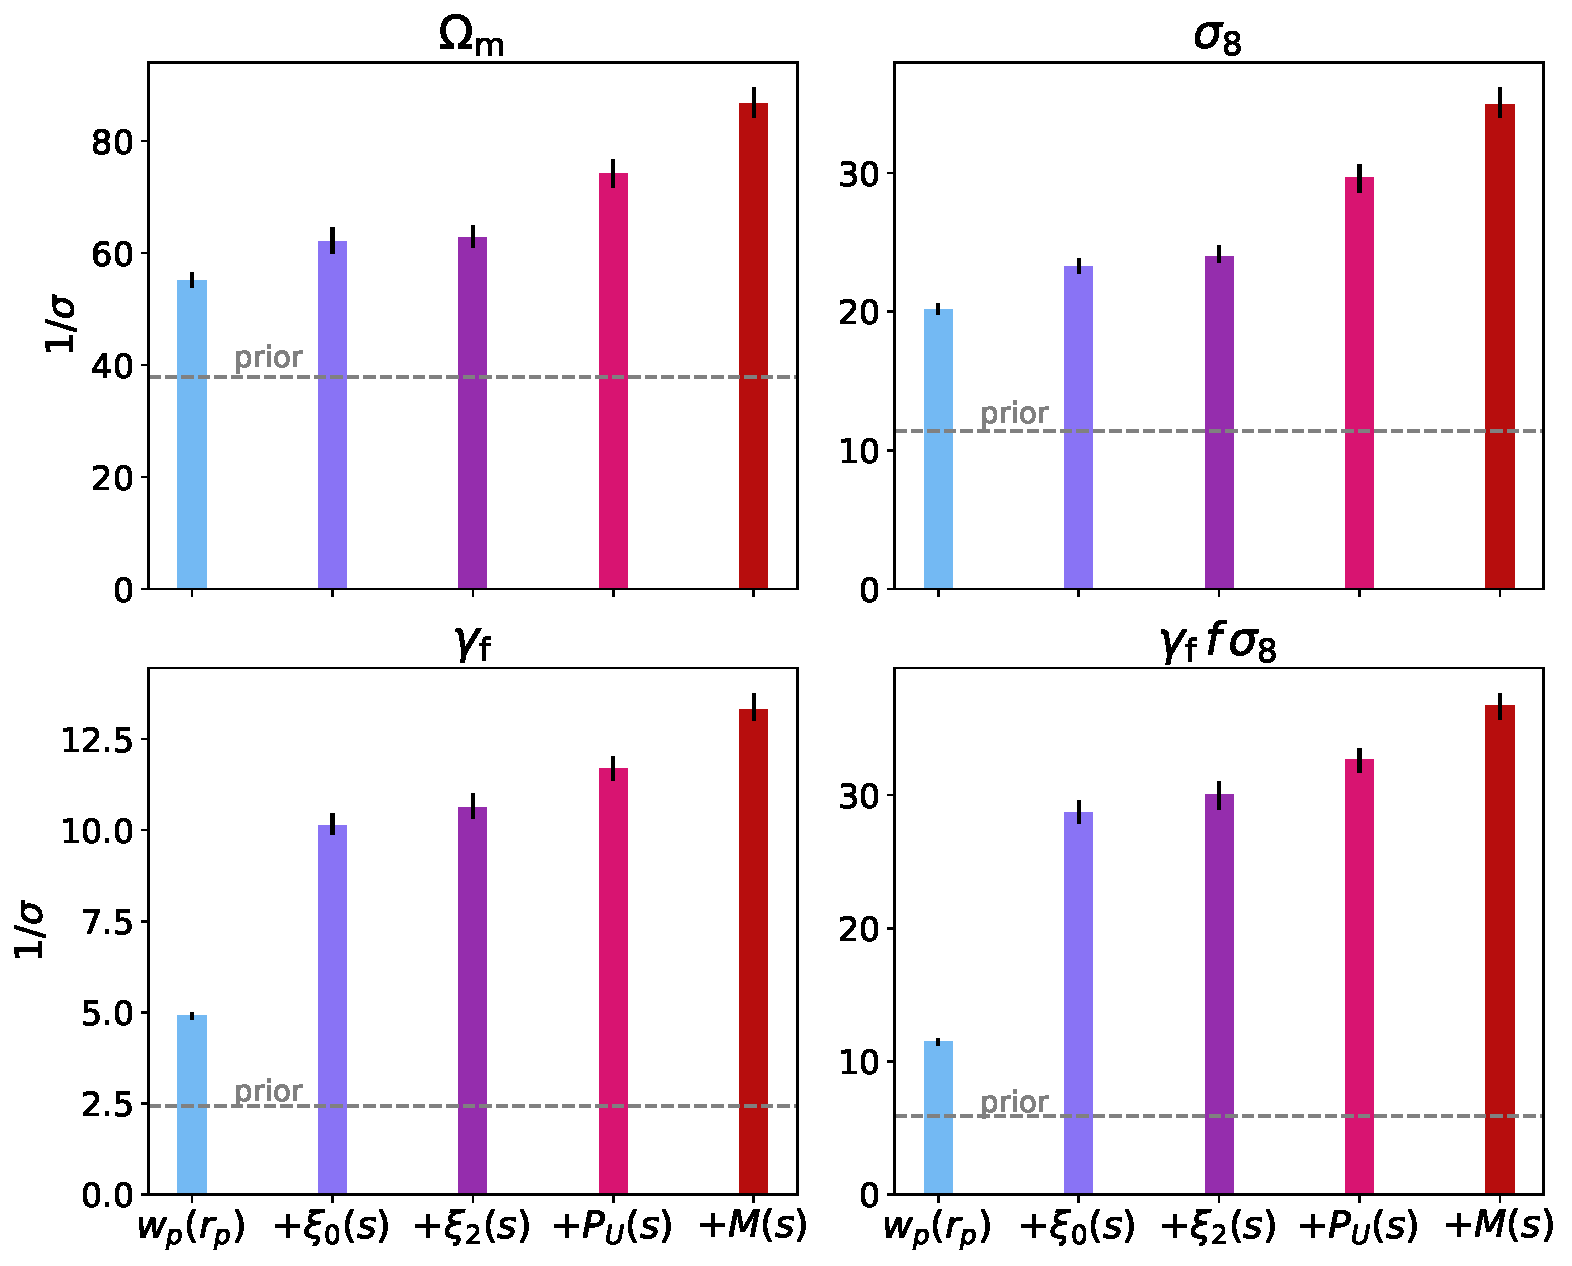
\includegraphics[width=0.48\textwidth]{recovery_addin}}
\caption{The precision of recovery tests for key parameters, averaged over the 70 test models. The quantity 1/$\sigma$ is the inverse uncertainty on the posterior marginalized over the other parameters, with $\sigma$ defined as the symmetrized inner 68\% region. The precision using only the prior is shown by the grey dashed line. Black bars shown the uncertainty on  1/$\sigma$ using bootstrap estimation. Panel (a) shows the precision for tests with single observables, and panel (b) for successively adding in each observable.}
\label{fig:recovery}
\end{figure*}

\subsection{Statistical results of recovery tests}
\label{sec:recovery_statistical}

We perform this MCMC inference for all 70 of our recovery test models (7 cosmologies populated with 10 unique HODs each, averaged over the 5 realizations).
For each parameter, we compute the uncertainty $\sigma$ on the posterior, defined as the symmetrized inner 68\% confidence region, marginalized over the other parameters.
In Figure~\ref{fig:recovery_single}, we show the inverse uncertainty $1/\sigma$ for each of the key cosmological parameters, including the combined quantity $\gfs$, averaged over all 70 test models, when using each of the statistics alone for the inference.
Note that larger bars indicate tighter constraints.
We compare this to the uncertainty obtained when just using the prior.
We see that all of the statistics on their own provide additional constraining power over the prior, for all parameters: $\wprp$ provides the most information for $\om$, $\sig$, and $\gf$, and $\cfm$ constrains $\gfs$ the most strongly.
The amount of information from $\wprp$ is significantly higher than found by other analyses (e.g. \citealt{Lange2022}); we find that this is largely a result of our choice to integrate out to only $40\,\hMpc$ along the line of sight, which preserves information in RSDs.
We test integrating out to $80\,\hMpc$ and find much less information content in $\wprp$ alone, though it still contains some.
For the beyond-standard statistics, it is noteworthy that $\upf$ and $\mcf$ do provide information on their own, particularly $\upf$ for $\om$ and $\mcf$ for $\gf$. 

We next perform recovery tests adding in each observable one at a time for the full test suite.
We show the results in Figure~\ref{fig:recovery_addin}, again for the mean of 70 test models.
We see that the inverse uncertainty monotonically increases as we add in additional observables.
Our main result is that the constraining power increases significantly between using only the combined standard observables, $\wprp$+$\cfm$+$\cfq$ (purple), and when adding in the beyond-standard statistics as well, $\wprp$+$\cfm$+$\cfq$+$\upf$+$\mcf$ (dark red).
The change in precision for these two cases tells us the amount of additional information contained in these new statistics: 
The precision increases (defined as the fractional decrease in the uncertainty $\sigma$) by 28\% for $\om$, 33\% for $\sig$, 20\% for $\gf$, and 18\% for the combined growth of structure parameter $\gfs$.
These are significant increases given the current precision of cosmological measurements.

\begin{figure*}%[htp!]
\centering
\subfloat[\label{fig:cdf_single}]{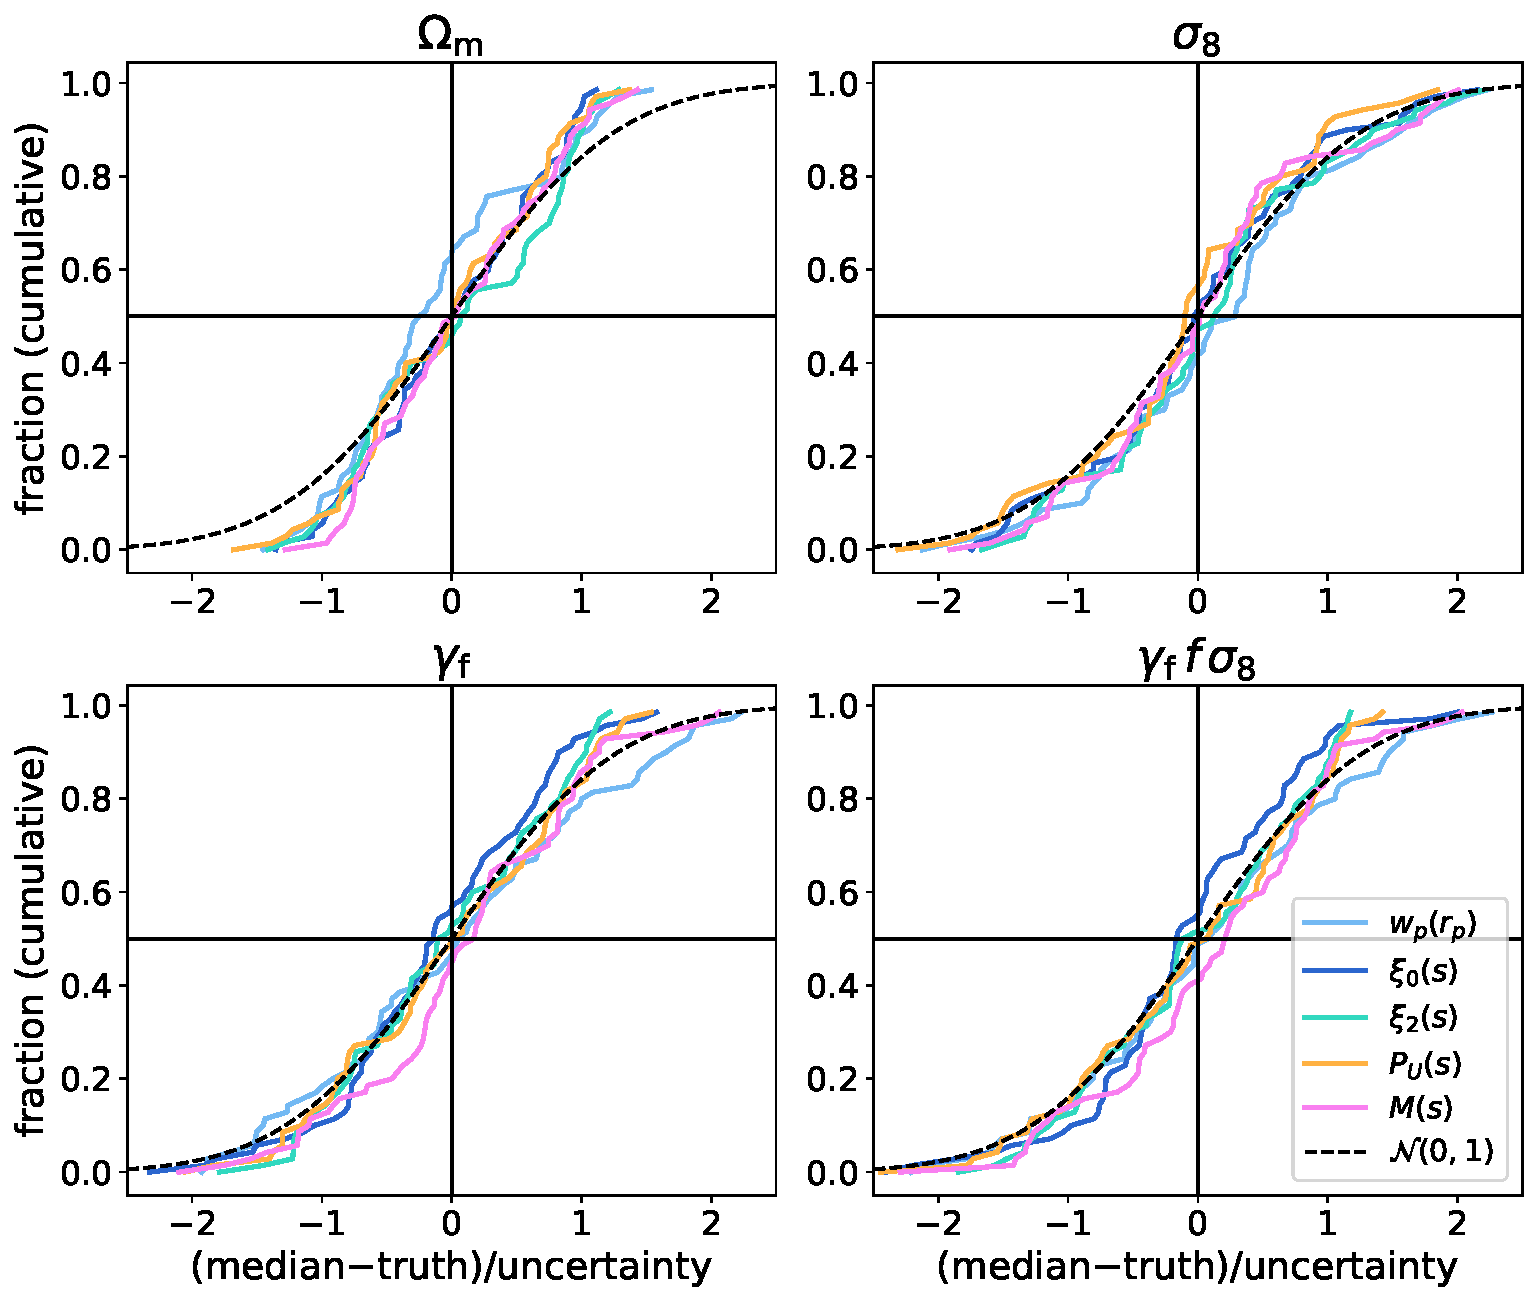
\includegraphics[width=0.46\textwidth]{cdf_single}}
\hspace{0.06\textwidth}
\subfloat[\label{fig:cdf_addin_wpmaxscale6}] {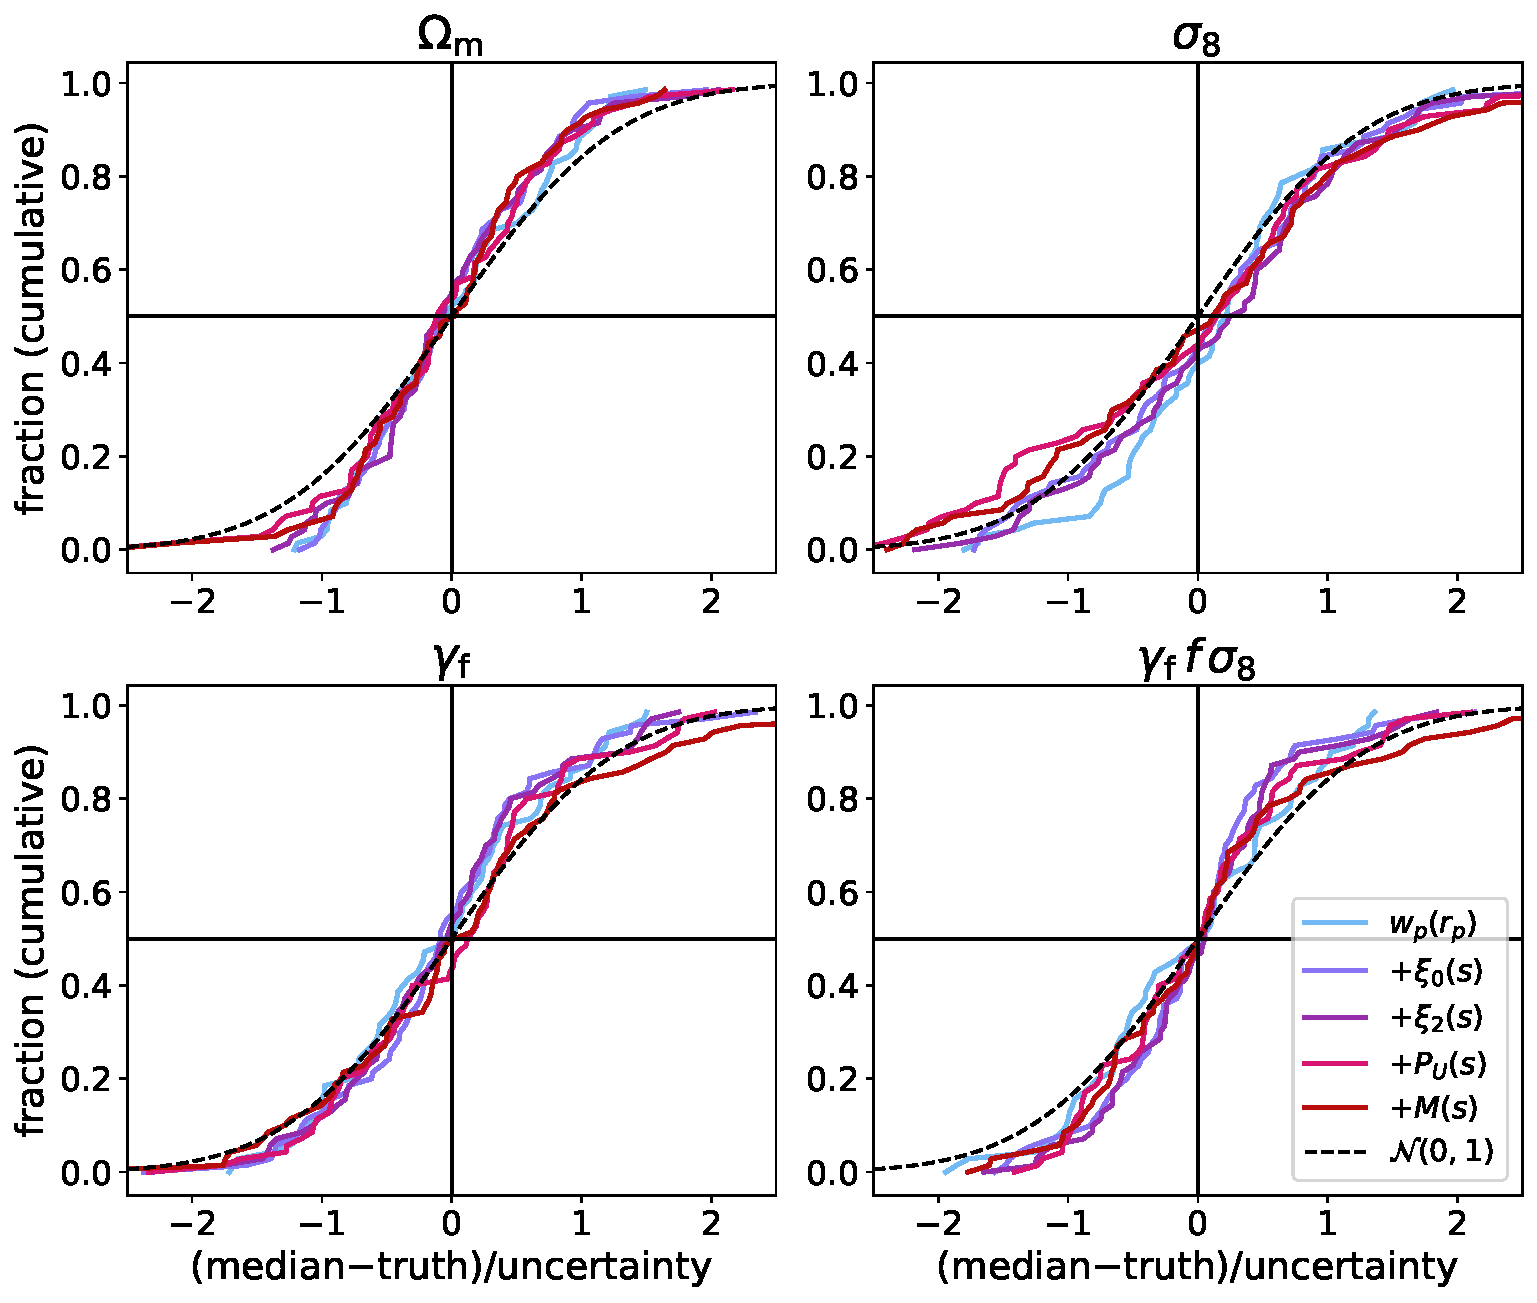
\includegraphics[width=0.46\textwidth]{cdf_addin_wpmaxscale6}}
\caption{Cumulative distribution functions (CDFs) of the differences between the true parameter value and the median of MCMC chain samples, divided by the uncertainty $\sigma$. Panel (a) shows CDFs for each of the observables on their own, and panel (b) adding in the observables successively; panel (b) excludes the two largest-scale $\wprp$ bins from all combinations, because of a bias discussed in the text. The dashed line shows the CDF of a unit normal distribution for comparison.}
\label{fig:cdf}
\end{figure*}

We assess the accuracy of the recovered parameters by computing the cumulative distribution function (CDF) of the error on the inferred parameter (difference between the median and truth), normalized by the uncertainty, for the 70 recovery test models.
Figure~\ref{fig:cdf_single} shows this CDF for each of the observables used for inference on their own.
We find that for most of the parameters of interest, the CDF follows a unit normal distribution, which is an indication that the recovery is unbiased.
(We note that the CDF is not an ideal statistic to measure bias, as the function values are dependent on all previous values, but a histogram with only 70 samples is too noisy to make statements about accuracy.)
The exception is $\om$ when using $\wprp$; we find that the distribution is biased by $\simo0.5\sigma$ to lower values of $\om$.
This is small but surprising, as it is such a standard statistic.

We investigate this issue by excluding successively larger scales of $\wprp$ from our analysis, as large-scale clustering should be the most affected by $\om$.
We find removing the two largest-scale bins, above 12.5 $\hMpc$ (with logarithmic averages of 17.7 and 35.4 $\hMpc$) results in an unbiased CDF of recovered $\om$ values.
To see if the issue could be attributed to small-number statistics, we run a larger set of recovery tests with $\wprp$ as the sole observable (including all bins), using the full 700-model test suite (each of the 7 cosmologies populated with the same 100 HOD models).
We compute the CDF of these 700 results and see that the same bias towards low $\om$ values persists.
With this larger sample, the histogram is less noisy, and the bias is small but clearly visible in the histogram as well.
One possibility is that there are degeneracies with other cosmological or HOD parameters that contribute to $\wprp$ favoring lower $\om$ values, but this is difficult to disentangle.

We check the effect of this bias on the precision of the recovered parameters by rerunning our recovery tests excluding the two largest-scale bins from $\wprp$ (but including these bins for the other observables that use them).
We find that when excluding these scales, the precision we obtain on $\om$ using only $\wprp$ decreases by less than 5\% (averaged over 70 test models); this is similar when using the three standard statistics, as well as when including all five statistics.
For the quantity $\gfs$, removing these two bins does significantly decrease the precision by $\simo40$\% when using only $\wprp$, but when including the other statistics in the inference, the change is only at the 3\% level.
This corresponds to a change in our main result, the increased precision when including the beyond-standard statistics to $\gfs$, of only 3.3\%.
These changes are quite small, and while it is curious that these two bins have significant power to affect the accuracy of the recovered $\om$ parameter yet not the precision, this small bias does not change our main result. 
Finally, we note that there is also a very small bias towards high $\sig$ when using just $\wprp$, which does not change when removing the two largest-scale bins; however, it does mostly disappear using the larger 700-model test sample, so we are not greatly concerned with this result.

We show the CDF when using combinations of successively more observables in Figure~\ref{fig:cdf_addin_wpmaxscale6}.
Here we have excluded the two largest bins of $\wprp$ for all recovery tests.
We note that when we do include all $\wprp$ bins, the recovery of $\om$ for all the combinations (which all contain $\wprp$) remains biased to the same level as seen with just $\wprp$.
As this bias is small and contained, as explained above, we still include these large scales in the rest of our analysis.
We find that these distributions are now generally unbiased for all of the cosmological parameters.
A slight bias to high $\sig$ is visible, most significantly for $\wprp$ and less so the other combinations.
Based on our analysis of the bias in $\om$ with $\wprp$, we expect that this even smaller bias will not change our final results, though future work should investigate this further.
The CDFs for these combined-observable results generally follow the unit normal distribution.
Both $\om$ and $\gfs$ show distributions slightly tighter than the normal distribution, indicating that we have overestimated our errors.
This means that our errors may be conservative, but the difference is small and we do not expect this to have significant effects on our results.



\subsection{Scale dependence}
\label{sec:scaledep}

\begin{figure*}
\centering
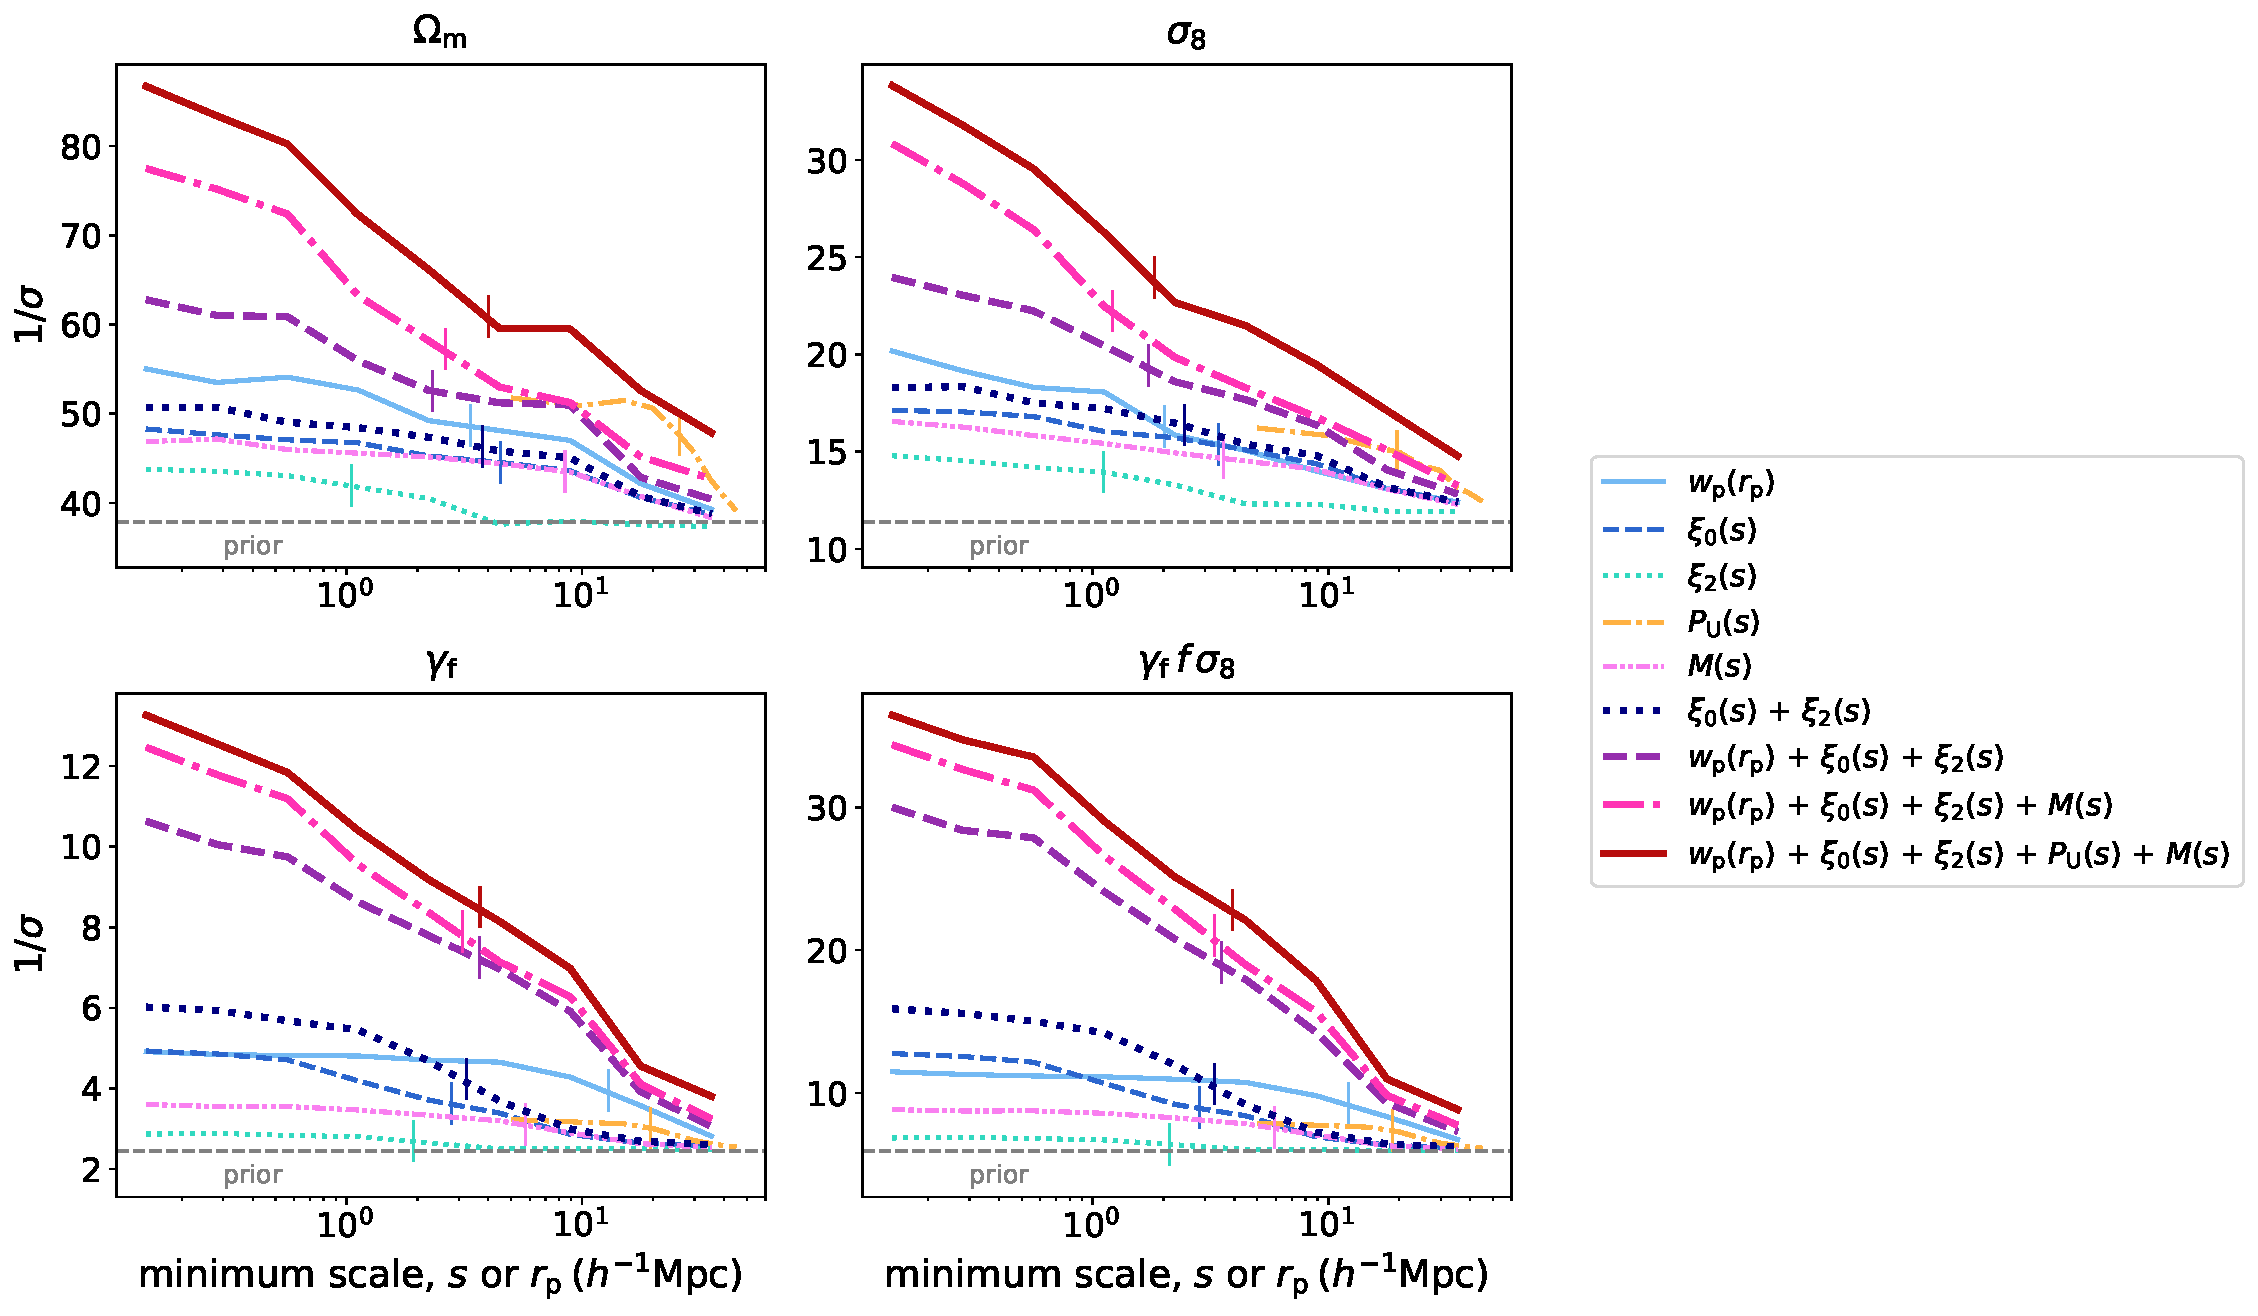
\includegraphics[width=0.9\textwidth]{scale_dependence}
\caption{The precision of recovery tests as a function of the minimum scale used in the analysis, averaged over the 70 test models. The maximum scale remains fixed at the maximum bin value. The precision is shown for chains using a single observable, as well as for several multi-observable combinations. The vertical bars indicate the scale at which half of the constraining power for that observable is in larger scales and half in smaller scales. Note that $\upf$ is measured on different scales than the other observables, from $5-45 \, \hMpc$, so at a minimum scale below $5 \, \hMpc$ it results in an overall shift in precision.}
\label{fig:scale_dependence}
\end{figure*}

We investigate the dependence of our parameter constraints on the scales used in the inference.
To analyze the contribution of small scales, we vary the minimum scale bin used and re-run the MCMC chains, for each parameter individually as well as the five-observable combined constraint.
The results are shown in Figure~\ref{fig:scale_dependence}, averaged over the 70 test models.
We note that the $\upf$ uses a different binning scheme than the other observables, so it is only shown on the scales on which it is computed, $5-45 \, \hMpc$, and when it is included in combination with the other observables, it results in an overall shift in precision below $5 \, \hMpc$.
For this reason, we add the $\upf$ and $\mcf$ in the opposite order as the rest of this paper.
We also include using just the combination $\cfm + \cfq$, as many analyses do.
Similarly, we run recovery tests varying the maximum scale.
The $1/\sigma$ lines for the minimum and maximum scale variation will cross each other at a particular scale; this scale is marked by a vertical bar, and indicates the scale at which equal information is provided by scales smaller than and larger than this scale.
Thus, a vertical bar far in the small scale regime means that most of the information comes from small scales (as only the smallest scales are needed on their own to equal the information content in all the larger scales), and conversely, a vertical bar at large scales means that most information comes from large scales. 

As we include smaller scales, the precision increases monotonically.
Using the vertical bars described above, we find that for $\gfs$ for the 4-observable constraint, scales from $0.1-4 \, \hMpc$ provide as much information as the scales $4-50 \, \hMpc$.
We also find that significant amounts of information are added all the way down to the smallest bin with minimum scale $0.1 \, \hMpc$.
This is a remarkable finding given that previous analyses either have not pushed to scales this small, or did not find as significant a contribution from small scales; we discuss this further in \S\ref{sec:discussion_aemulus}.

To understand this result, we look at the constraints from individual observables for $\gfs$.
For $\cfq$, half of the information comes from scales below 2 $\hMpc$; for $\cfm$, below 3 $\hMpc$; for $\mcf$, below 6 $\hMpc$; and for $\wprp$, below $\simo10 \hMpc$ (for $\upf$, this is $\simo20 \hMpc$).
Given that $\cfm$ contains much more information than $\cfq$, it seems that $\cfm$ is driving the large amount of information on $\gfs$ at small scales, perhaps with contributions from combinations of the other observables.
We also look at the constraints on the individual key cosmological parameters $\om$, $\sig$, and $\gf$; for the five-observable constraint for each of these, half of the information comes from scales below $\simo 2-4 \, \hMpc$, indicating that small scales contribute to improved constraints on all of these parameters individually which in turn aids in constraining $\gfs$.
We also see that the contribution from small scales is less significant for observable combinations containing only standard statistics. 
For $\cfm + \cfq$, the precision nearly flattens out for scales below $\simo 1 \, \hMpc$ for all parameters.
Including $\wprp$ does add some constraining power at small scales, particularly for $\gf$ and $\gfs$.
Finally, adding in $\upf$ and $\mcf$ accesses a significant amount of additional information at smaller scales, particularly for $\om$ and $\sig$.

Notably, the significant additional constraining power adding in $\wprp$ to $\cfm + \cfq$ is different than the findings of \cite{Lange2022}, who found that it only marginally improved constraints.
Given that the effect of $\wprp$ is strongest for $\gf$ and $\gfs$ in our analysis, and \cite{Lange2022} do not include this velocity field rescaling parameter, it seems that the increase in constraining power we find is a result of the sensitivity of $\wprp$ to velocity information.
Indeed, we only integrate out to $\pi_\mathrm{max}=40\,\hMpc$, while \cite{Lange2022} uses a value of $\pi_\mathrm{max}=80\,\hMpc$.
We perform a test using this larger value, and find as expected that in this case $\wprp$ does not add much more constraining power to either $\gf$ or $\gfs$.
Thus we conclude that our choice of $\pi_\mathrm{max}$ preserves significant velocity information that allows $\wprp$ to constrain the growth of structure parameter through its dependence on the halo velocity field.


\subsection{Recovery tests on Uchuu mocks}

One important difference of our analysis compared to perturbation theory approaches is that the latter require a large number of nuisance parameters to model higher-order statistics such as the bispectrum (e.g. \citealt{philcox_cosmology_2022}).
Instead, we use the HOD, which is a more compact parameterization that incorporates more physically and empirically motivated assumptions about galaxy formation than perturbation theory does.
However, these assumptions have the potential to make our approach less flexible.
We thus test our approach on a catalog constructed with a different galaxy formation prescription that breaks some of these assumptions, namely Subhalo Abundance Matching (SHAM, e.g. \citealt{vale_linking_2004, kravtsov_dark_2004, conroy_modeling_2006}).
This is an important validation step before applying our emulators to real data.
When we adapt our emulators for the full data analysis, we will perform additional tests in this vein to ensure that our framework encompasses the range of expected galaxy formation scenarios.

For this test, we use mock catalogs generated from the Uchuu simulations \citep{ishiyama_uchuu_2021}, to additionally check that our framework generalizes beyond the \aemulus N-body simulations.
The Uchuu simulation we use has a mass resolution of $3.27 \times 10^7 \, h^{-1} M_\odot$ and a volume of $(2 \, \hGpc)^3$, nearly a factor of 8 larger than the \aemulus boxes, so the clustering statistic measurements are very precise.
To test that our approach is robust to our use of an HOD model with environment-dependent galaxy assembly bias, we instead populate the Uchuu simulations using the SHAM approach.
SHAM assigns galaxies to subhalos based on a rank-ordered relation between galaxy mass and subhalo mass, with some additional parameters to regulate the scatter, and is able to reproduce galaxy assembly bias to some extent.
We specifically use the SHAM method of \cite{lehmann_concentration_2016} to generate our Uchuu mocks.

For this test, we require a data covariance matrix for the Uchuu mock data.
As there is only one realization of the Uchuu simulation, we use the GLAM Particle-Mesh simulations \citep{KlypinPrada2018} for this purpose, which have many independent realizations; we use 986 boxes for our covariance estimate.
These are all at the same cosmology; we consider the covariance of the fractional differences from the mean for each statistic.
The GLAM boxes have a volume of $(1 \, \hGpc)^3$, so we rescale the covariance matrix for the Uchuu mock volume.
We use the emulator covariance matrix $ \cov{emu}$ described in \S\ref{sec:cov}, and add this to the data covariance to obtain to the final covariance matrix we use in the likelihood function.

We make a few tweaks to our emulation procedure for application to Uchuu.
First, we found that the range of the HOD parameter $\msat$ used for the \aemulus mocks is not large enough to fit the Uchuu data.
Thus, we extended the range of this parameter to $14.0 \leq \mathrm{log}(\msat) < 15.5$, generated a new set of mock catalogs from the \aemulus simulations, and reconstructed the emulators.
(Two of these mocks resulted in unphysical values of clustering statistics; we discarded these from our training set.)
We found that this did not change our emulator accuracy or recovery tests on \aemulus test simulations significantly. 
Second, some of the clustering statistics of the Uchuu mock data do not lie in the center of the statistics of our training set, leading to difficulty in ensuring the emulators explore the relevant region of parameter space.
To alleviate this, we chose the 2000 (out of 4000) training mock catalogs with clustering statistics closest to those of the Uchuu data, using a $\chi^2$ metric with the variance given by the diagonal of the GLAM covariance matrix used for the data covariance discussed above.
We then reconstructed the emulators with just these mocks, and used these in MCMC chains to recover the Uchuu parameters.
Finally, we faced the issue that the $\upf$ of the Uchuu data is on the edge of our training data set, as the training parameter space was chosen based only on standard summary statistics.
Because of this, the MCMC is unable to find a reasonable fit when including the $\upf$.
To address this, we inflate the error on the $\upf$ (the diagonals of that block of the covariance matrix) by a factor of two.
When we apply the framework to real data, we will have to ensure that our training set appropriately spans the space of all of the observables used, but this is sufficient for this proof-of-concept check.

\begin{figure*}
\centering
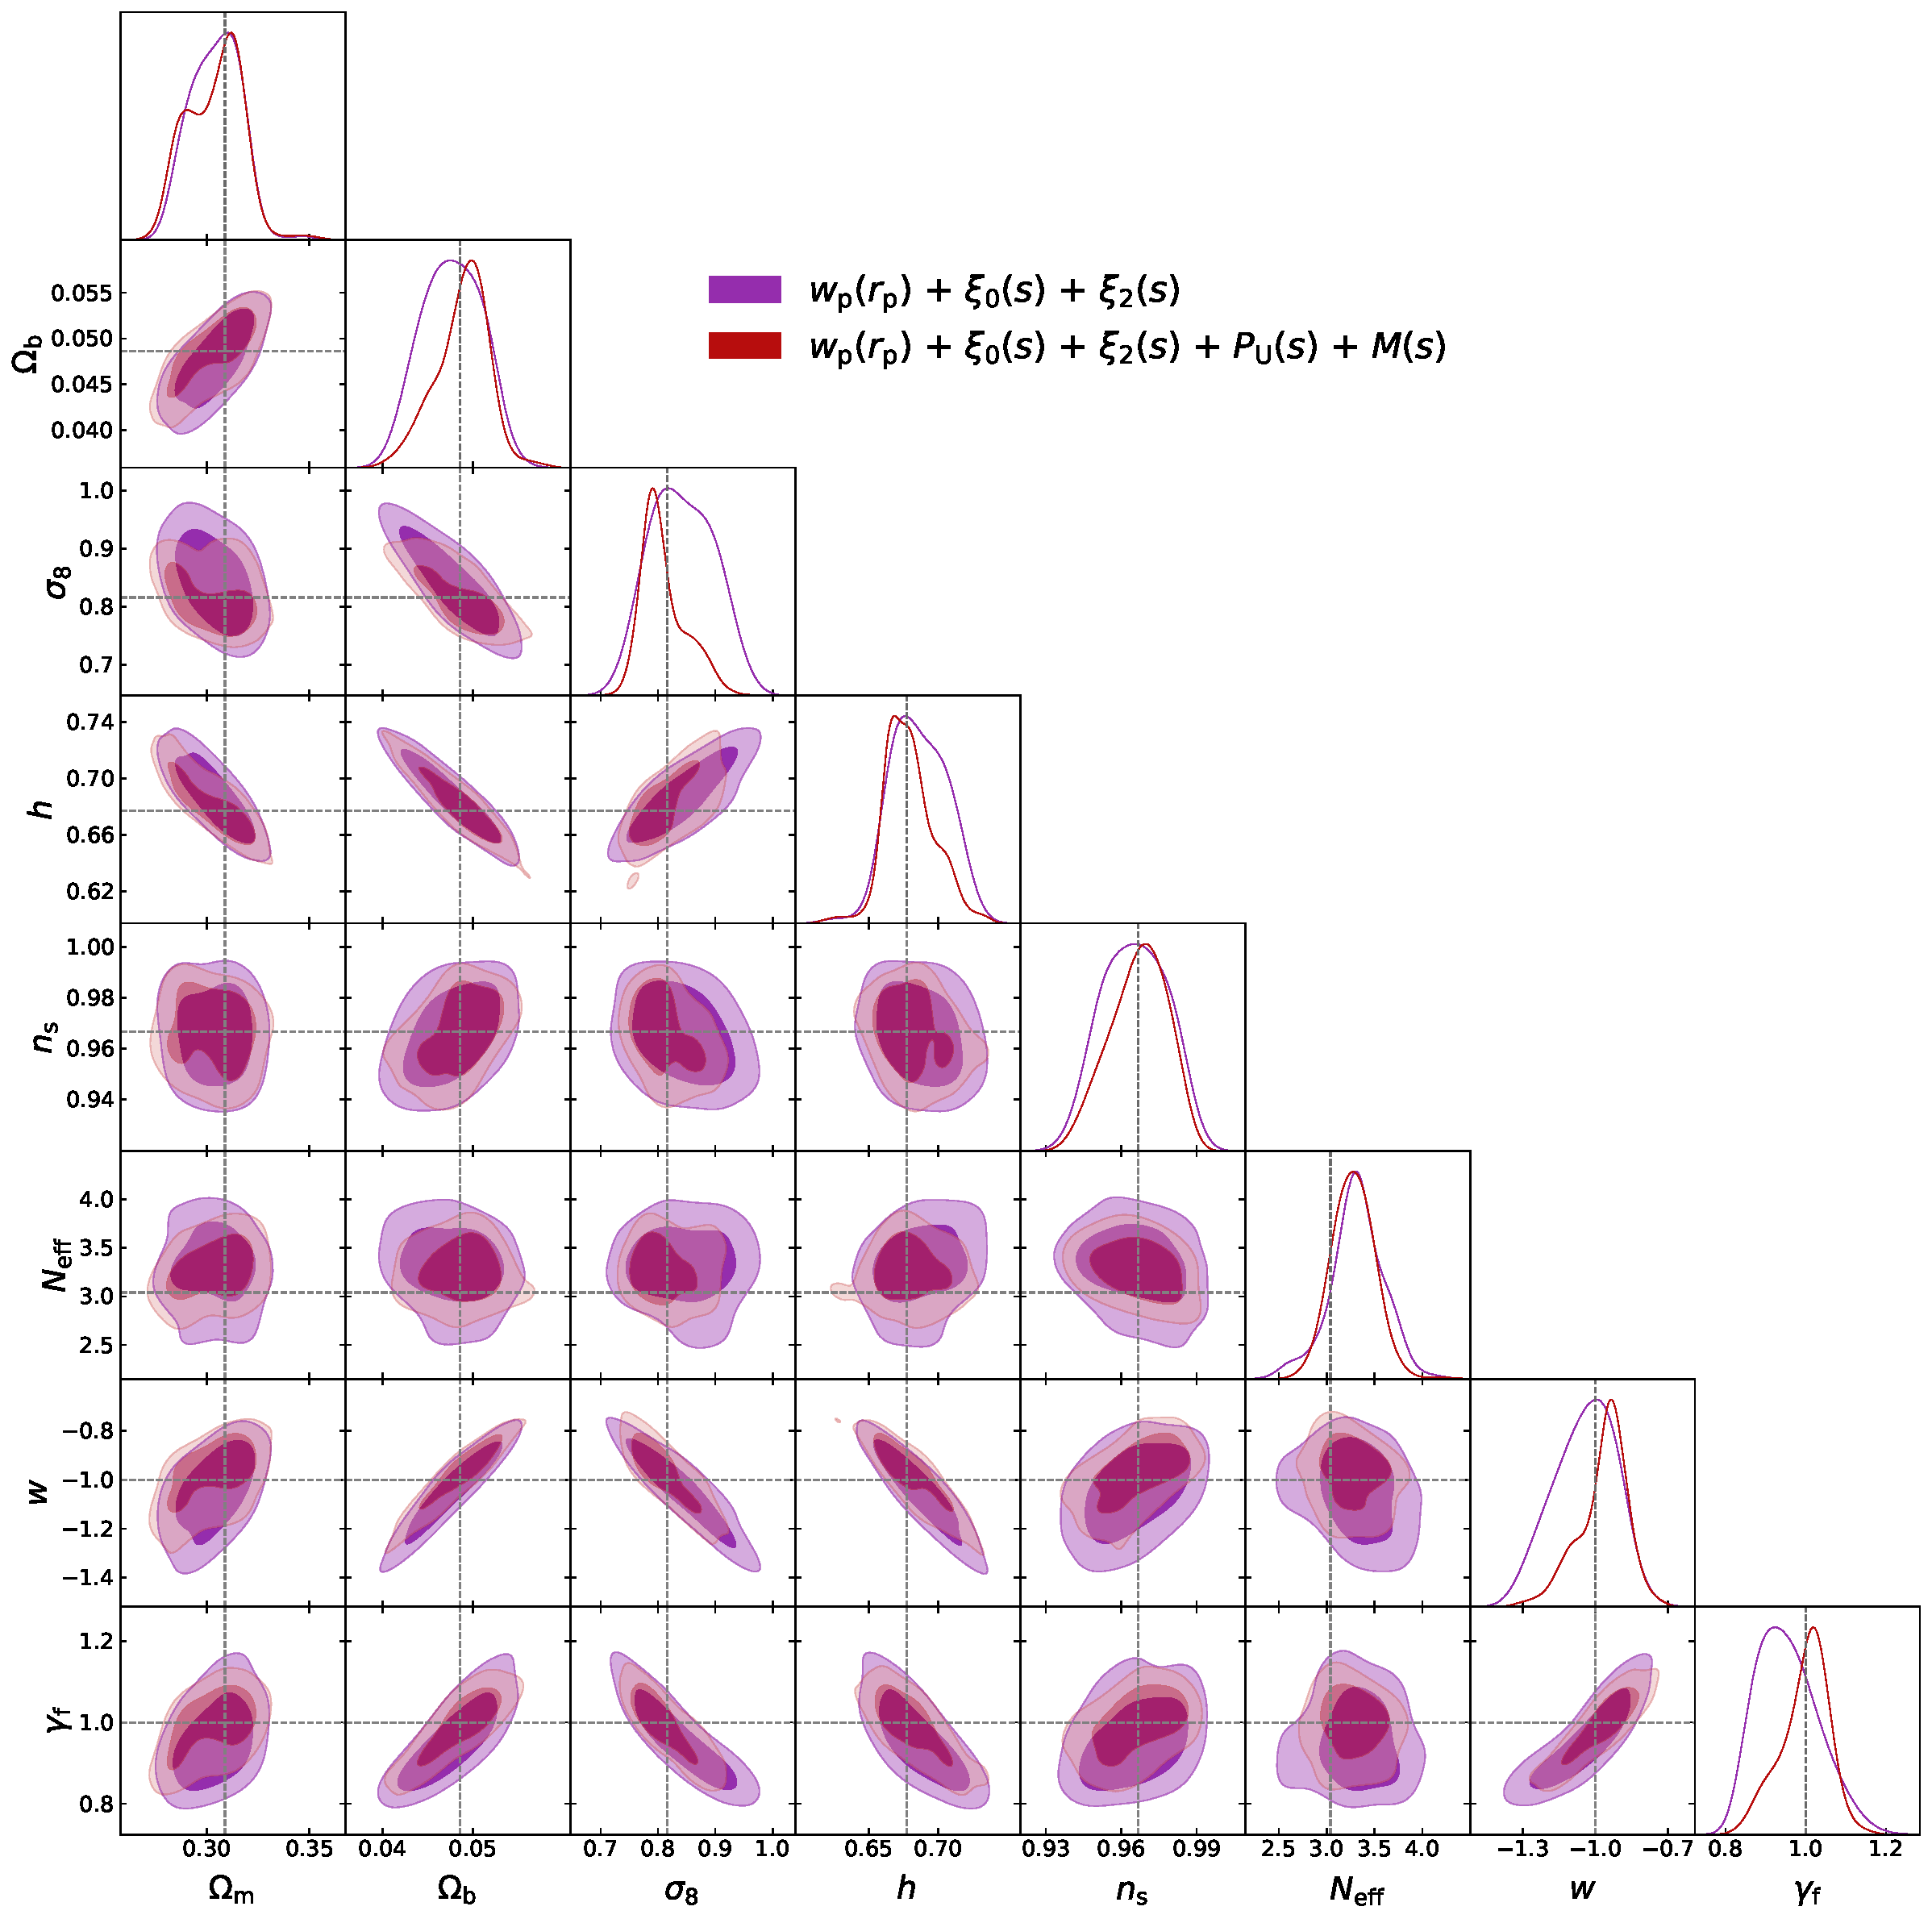
\includegraphics[width=0.6\textwidth]{uchuu_recovery}
\caption{Recovery test on the Uchuu mock catalog. Constraints are shown for all the cosmological parameters and $\gf$ when using just the standard statistics (purple), and when including the $\upf$ and $\mcf$; the true parameter values are shown in the dashed grey lines. The parameters are recovered accurately, with the beyond-standard statistics adding increased precision on most of the parameters.}
\label{fig:uchuu_recovery}
\end{figure*}

The results of our Uchuu recovery test are shown in Figure~\ref{fig:uchuu_recovery}, using just standard statistics and including the beyond-standard statistics.
We find that in both cases, we can accurately recover the Uchuu cosmological parameters, with the additional statistics adding constraining power for most parameters.
The final set of best-fit statistics using all five observables has a reduced $\chi^2$ of 1.16, and the cosmological parameters are recovered to within $0.5\sigma$, besides $N_\mathrm{eff}$ which is recovered to within $1\sigma$.
We also recover $\gf$ accurately (significantly more accurately than when using just the standard statistics).
The inclusion of the beyond-standard statistics results in an increase in precision of 34\% on $\sig$, similar to our findings with \aemulus recovery tests.
The precision on $\gf$ increased by 25\%, and on $h$ by 18\%. 
We note that the constraints on $\om$ and $\gfs$ get slightly worse when including $\upf$ and $\mcf$; this is likely related to the aforementioned issues with $\upf$, as tests with only the standard statistics and $\mcf$ show an improvement on $\om$ constraints (though the precision on $\gfs$ remains constant).
These results are promising for the application of this framework to real data sets.

When we apply the emulation approach to real data, we will ensure that the measured statistics fall well within the space of the statistics of the training models.
This will address both of the issues we found when performing this test, and ensure that we are able to find a good fit to the data.



\section{Additional Results and Tests}

\subsection{Full posterior plots}

\begin{figure*}[p!]%[htpb]
\centering
\subfloat[\label{fig:contour_addin_allcosmo}]{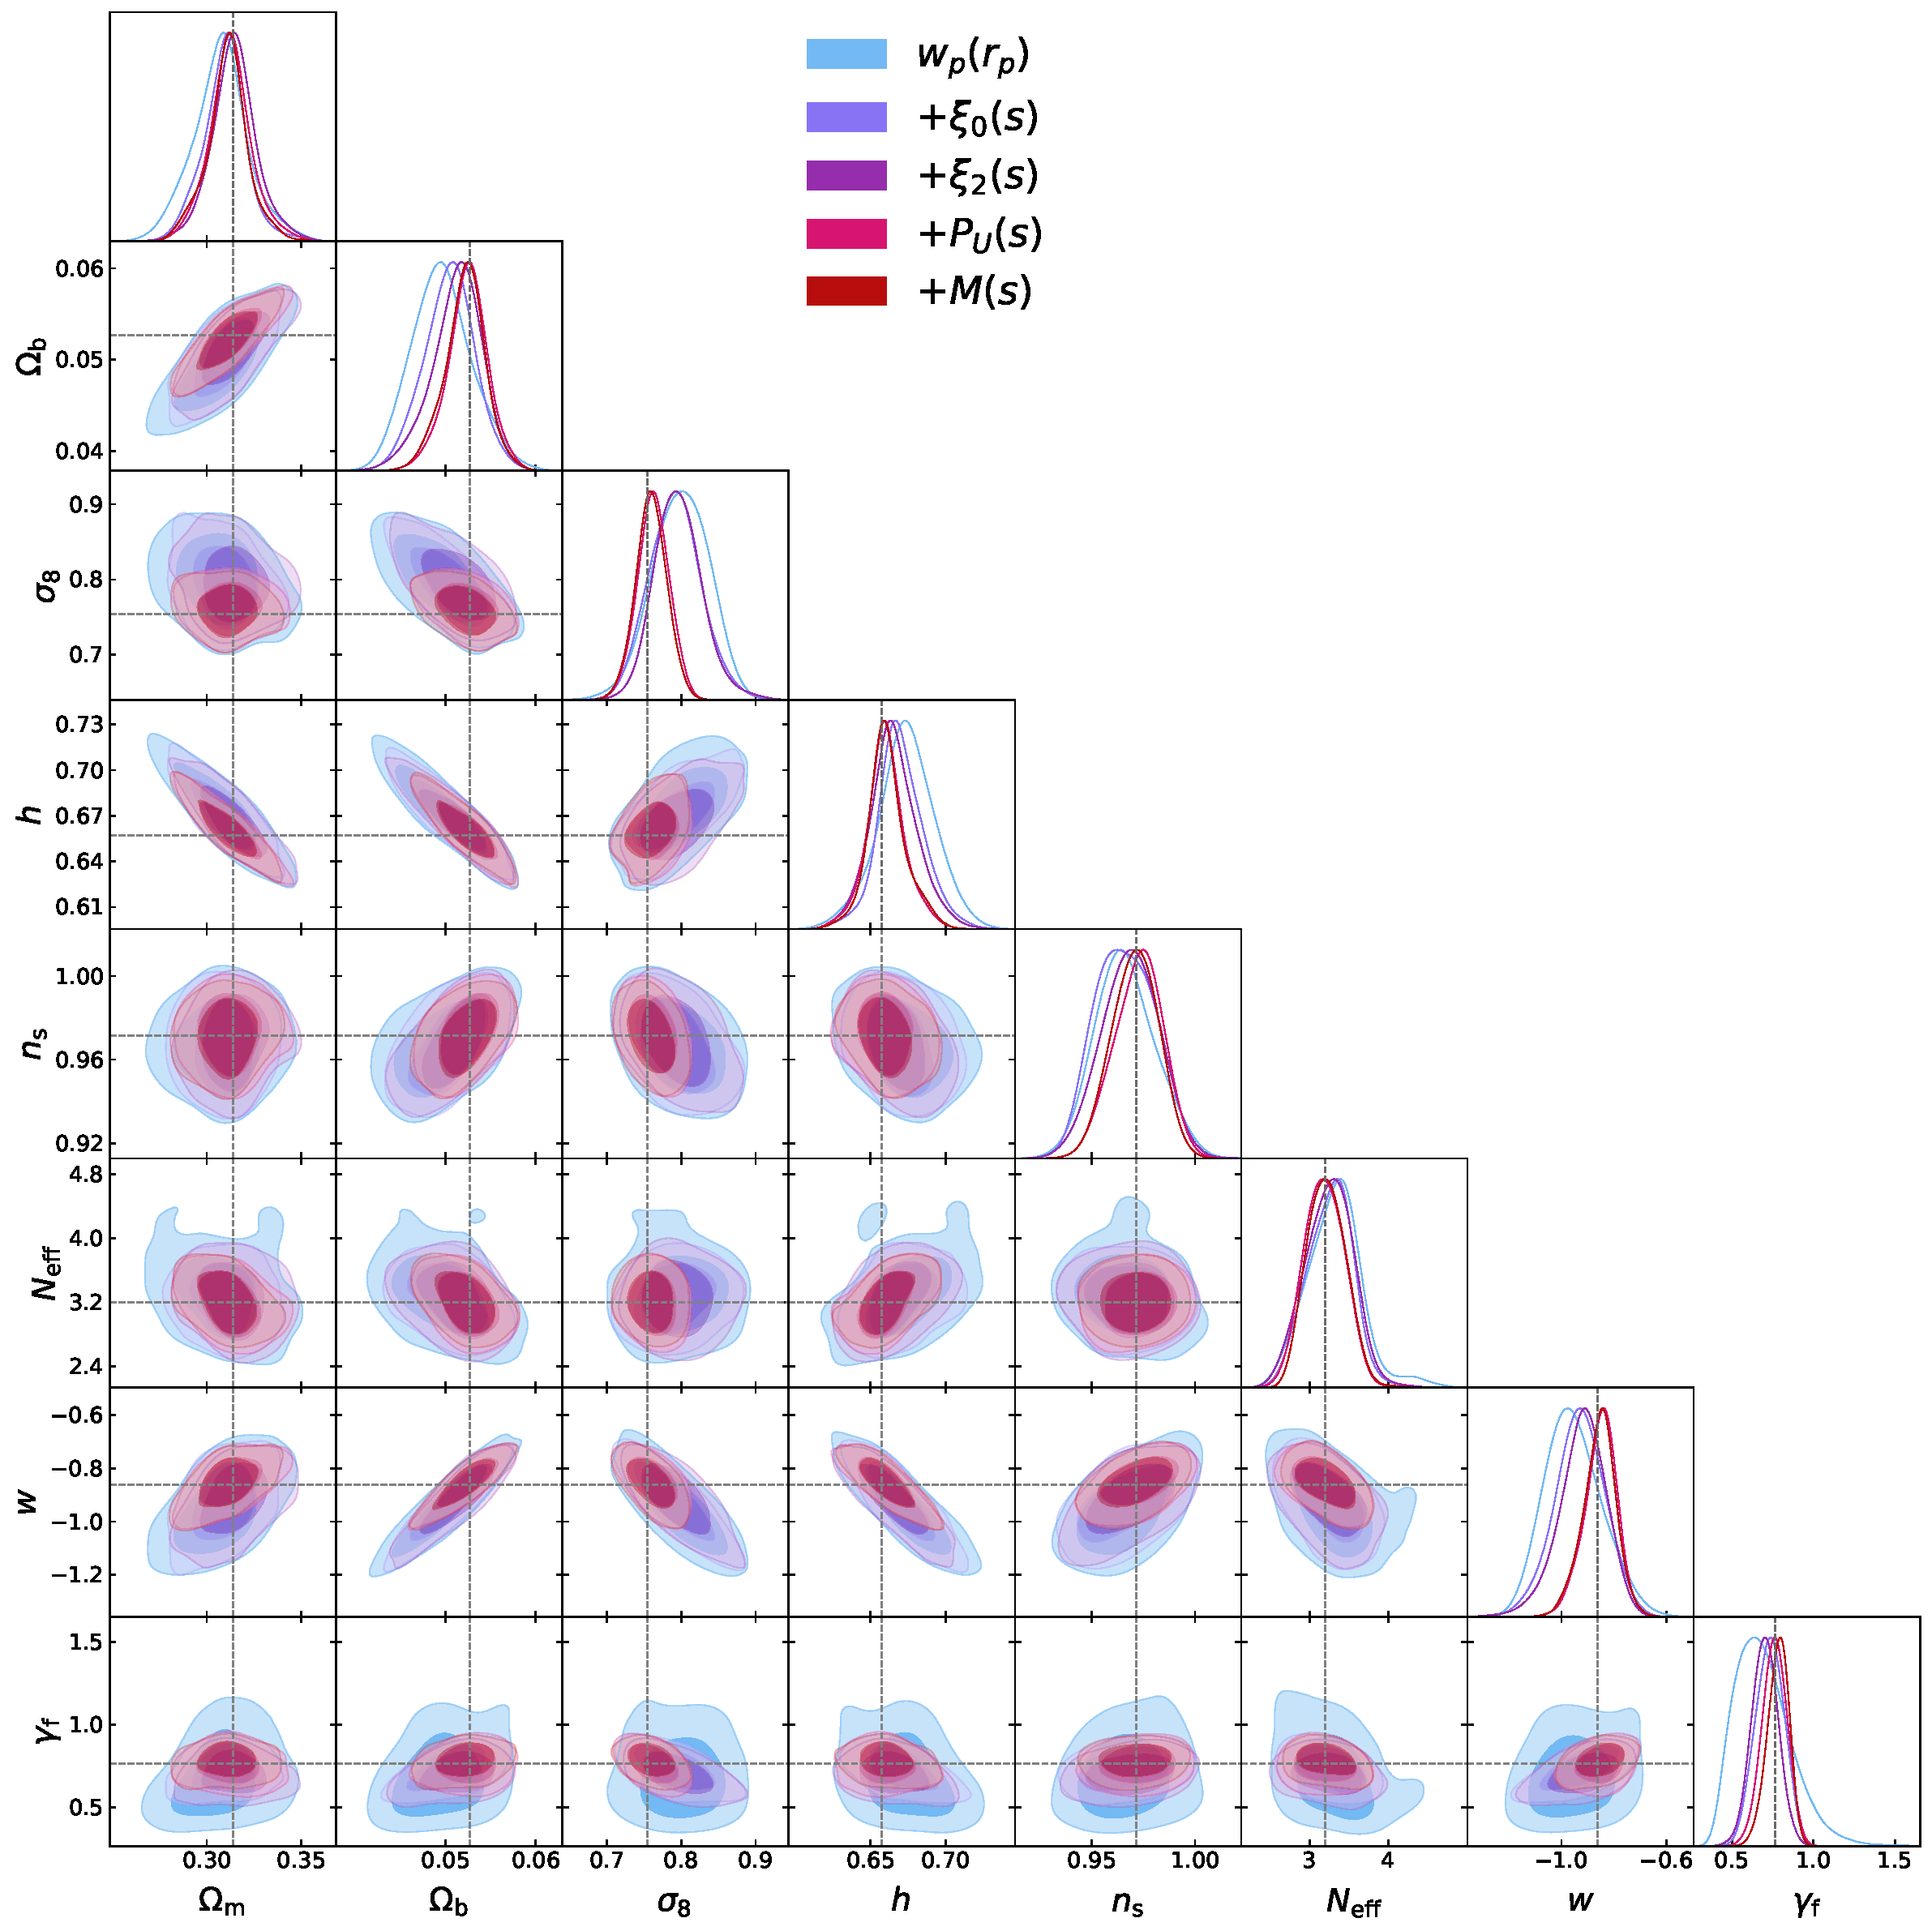
\includegraphics[width=0.6\textwidth]{contour_addin_allcosmo}}
\vspace{1em}
\subfloat[\label{fig:contour_addin_keymix}]{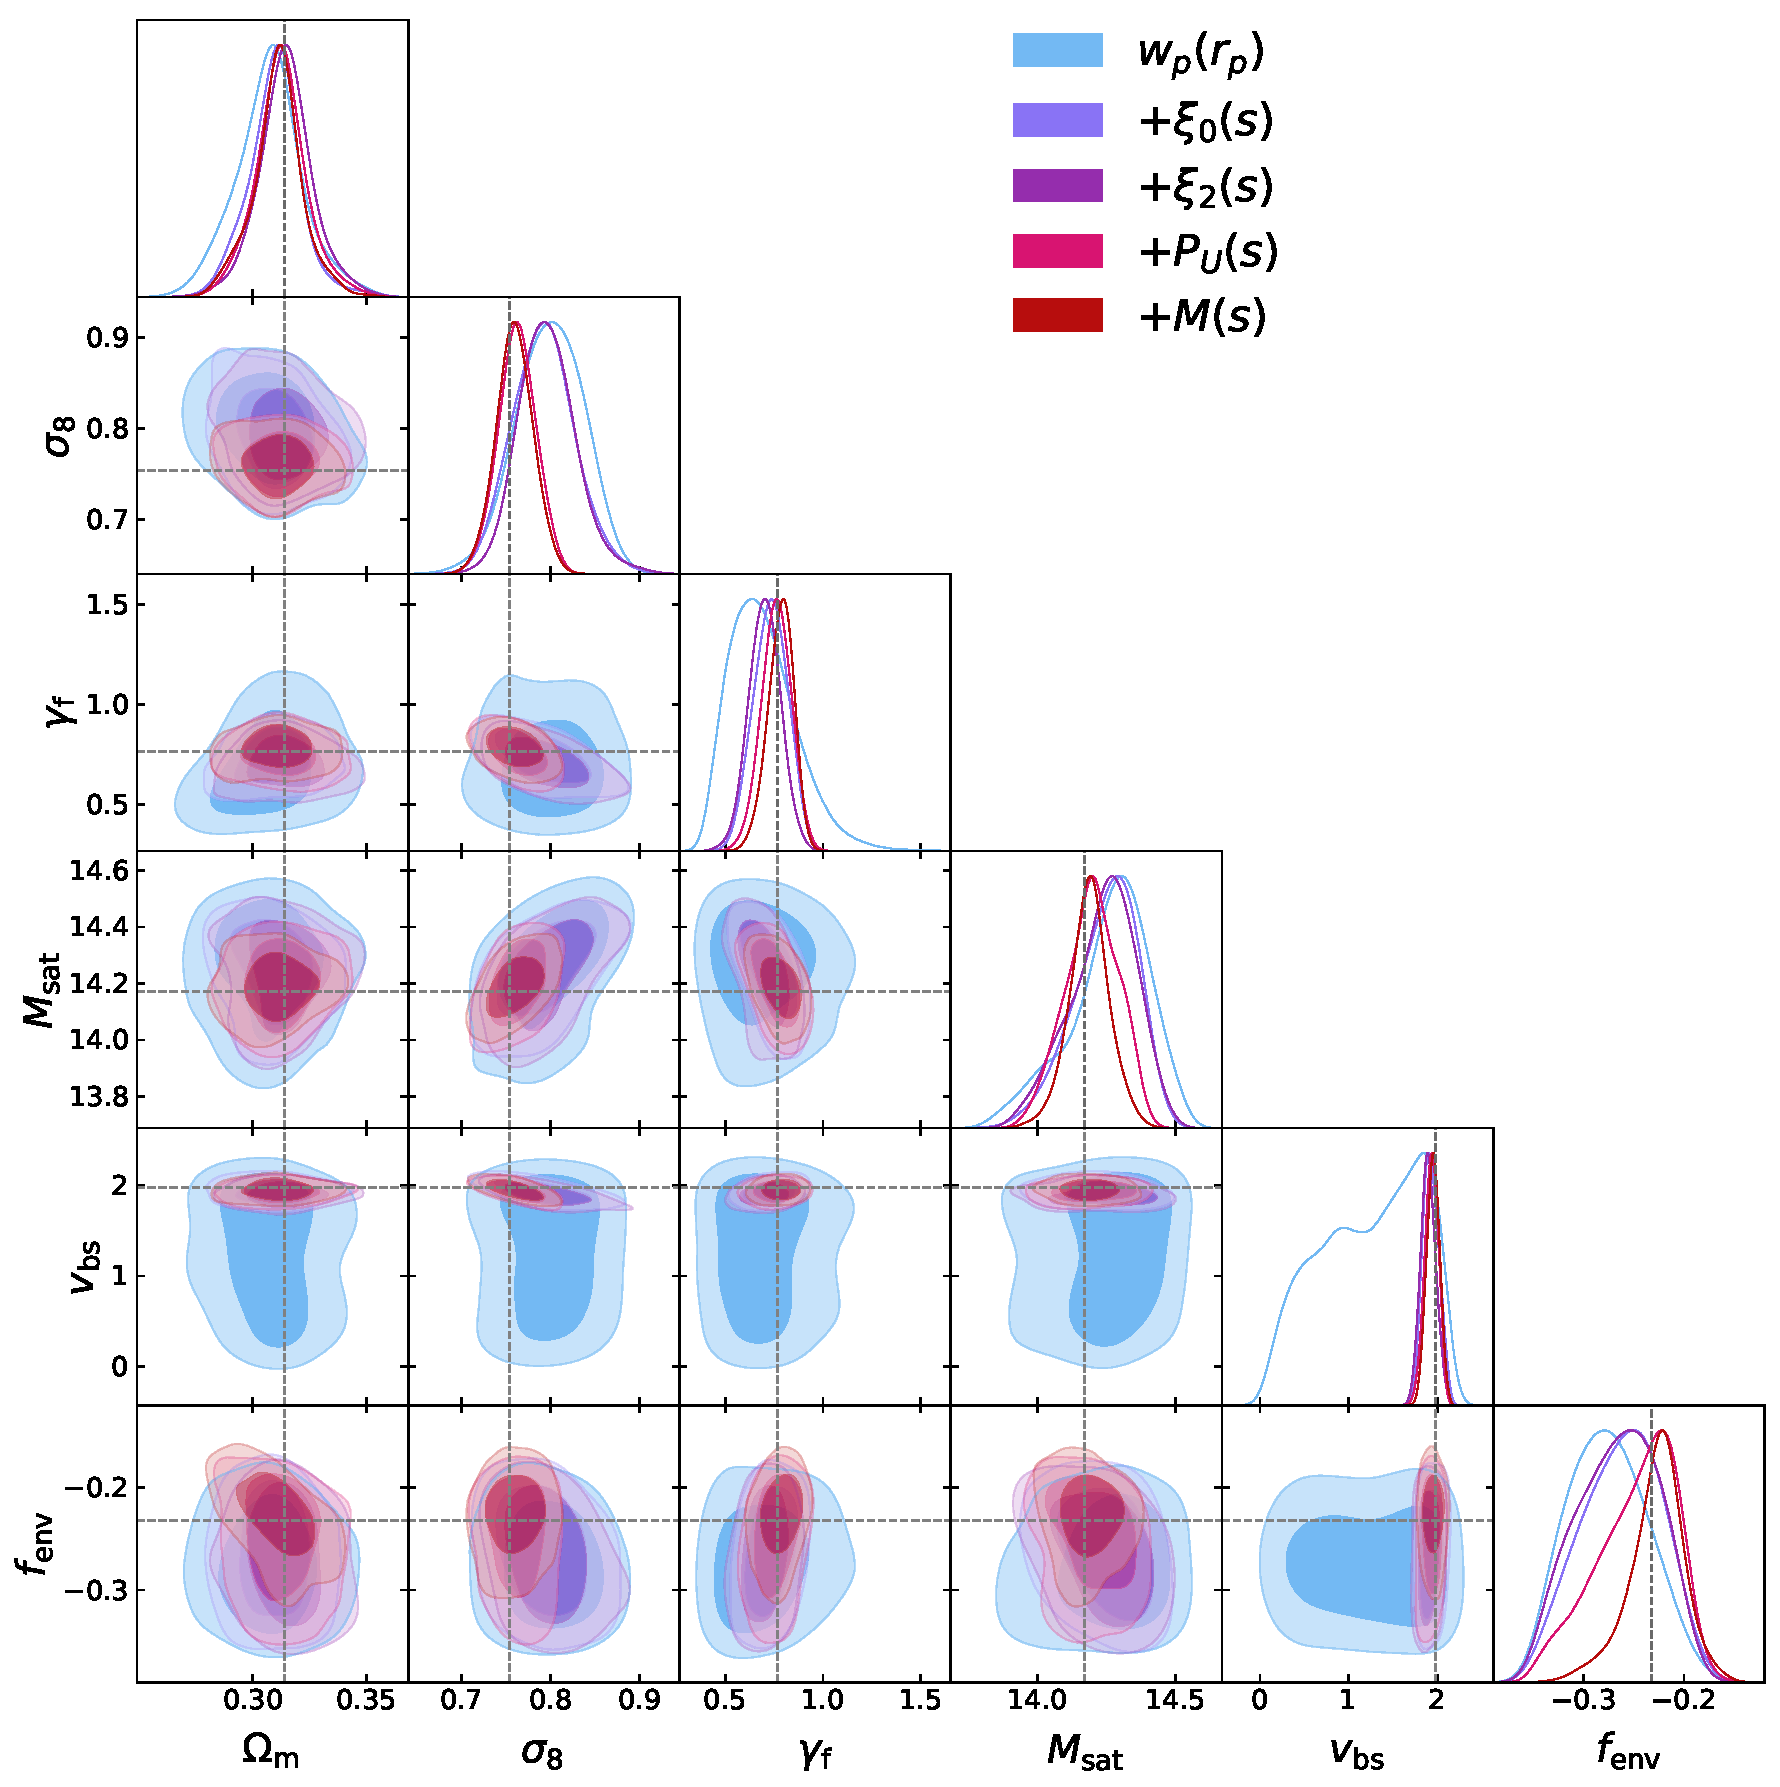
\includegraphics[width=0.5\textwidth]{contour_addin_keymix}}
\caption{Posteriors for all free parameters in our recovery test of a single cosmology+HOD model, when adding in observables successively. Contours are shown for (a) all cosmological parameters, (b) a mix of the key cosmological, HOD, and assembly bias parameters, and (c) all HOD and assembly bias parameters.}
\end{figure*}

\begin{figure*}[p!]\ContinuedFloat
\centering
\subfloat[\label{fig:contour_addin_allhodab}]{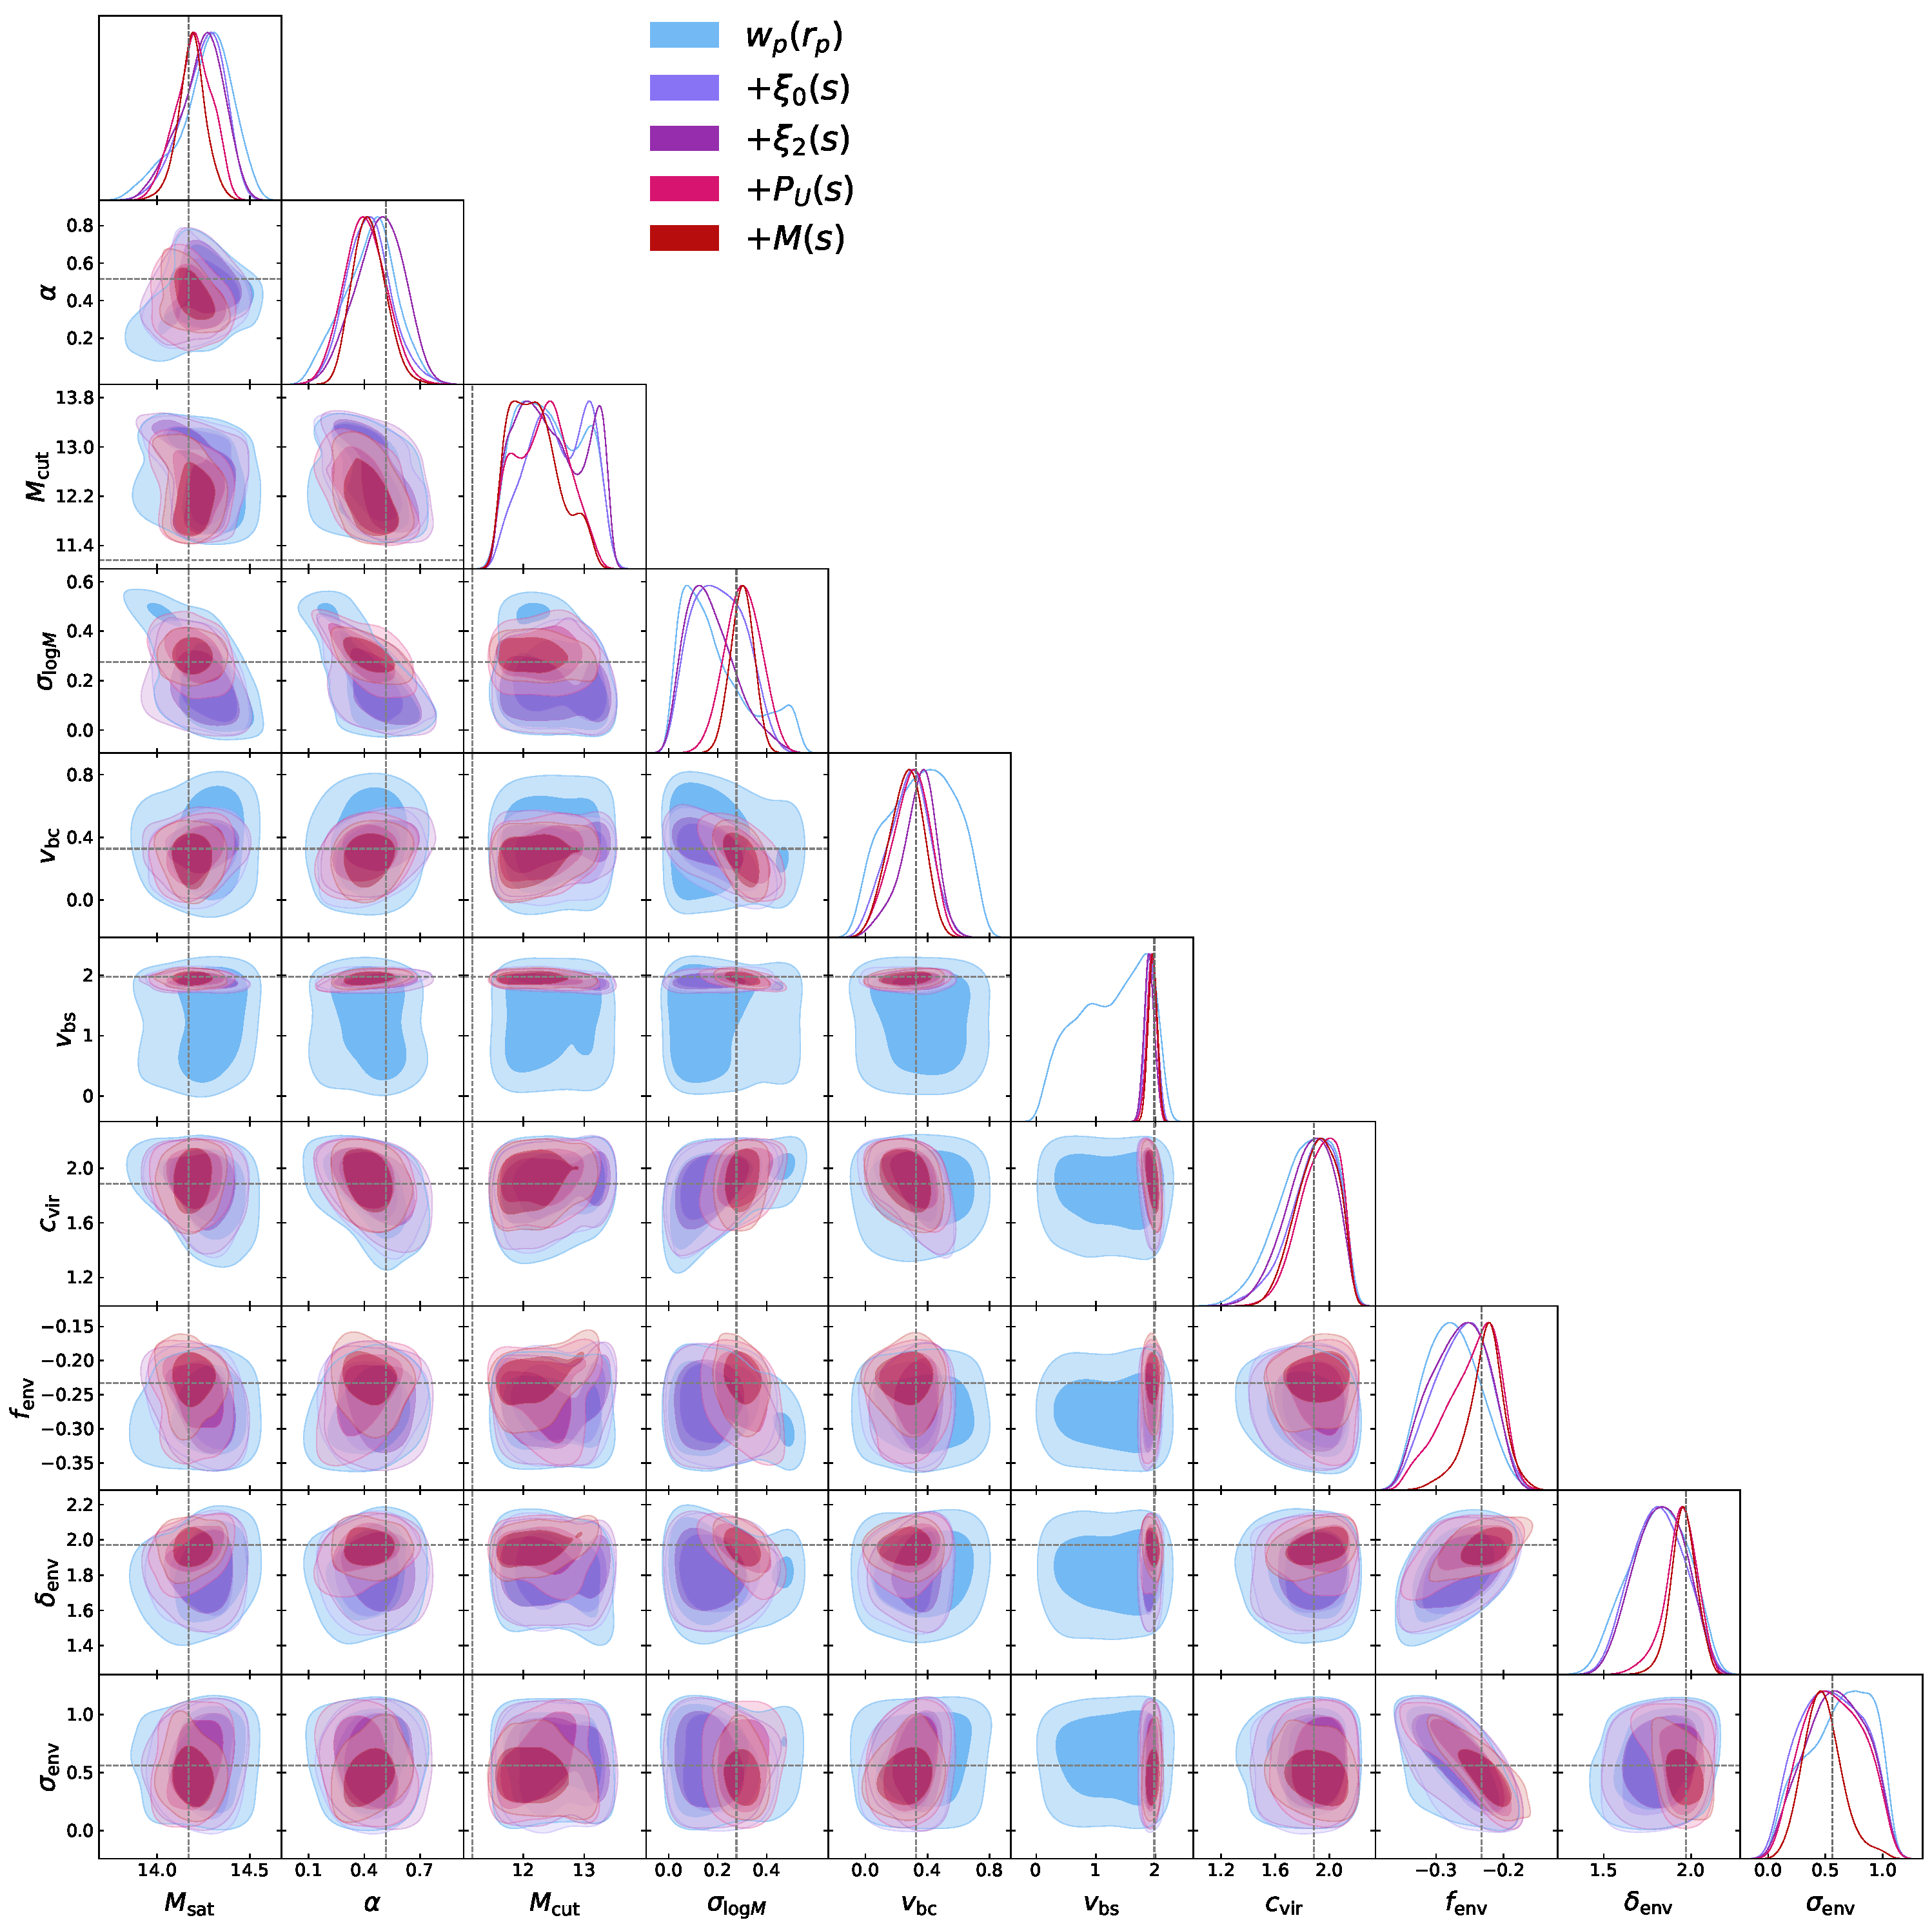
\includegraphics[width=0.8\textwidth]{contour_addin_allhodab}}
\caption{Continued from previous page.}
\label{fig:contours_full}
\end{figure*}

We show contour plots of all the recovered parameters for a single cosmology+HOD test model in Figure~\ref{fig:contours_full}, when successively adding in our observables.
In Figure~\ref{fig:contour_addin_allcosmo}, we show the cosmological parameters; in Figure~\ref{fig:contour_addin_keymix}, a combination of the key cosmological, HOD, and assembly bias parameters; and in Figure~\ref{fig:contour_addin_allhodab}, all the HOD and assembly bias parameters.
We can clearly see the degeneracies between many of the parameters here, and for many of these, including the beyond-standard statistics breaks the degeneracy. 
This is true for degeneracies between cosmological parameters and HOD parameters, as with $\sig$ and $\msat$; between HOD parameters, as with $\vbs$ and $\sigma_{\mathrm{log}M}$; and between assembly bias parameters, as with $\fenv$ and $\sigma_\mathrm{env}$.
This helps explain how the combination of our flexible assembly bias model and the emulation of beyond-standard statistics improves our precision on cosmological parameter constraints.


\subsection{Covariance matrix comparison}
\label{appendix:cov}

\begin{figure*}[t]
\centering
\subfloat[\label{fig:contour_cov_c1h12}]{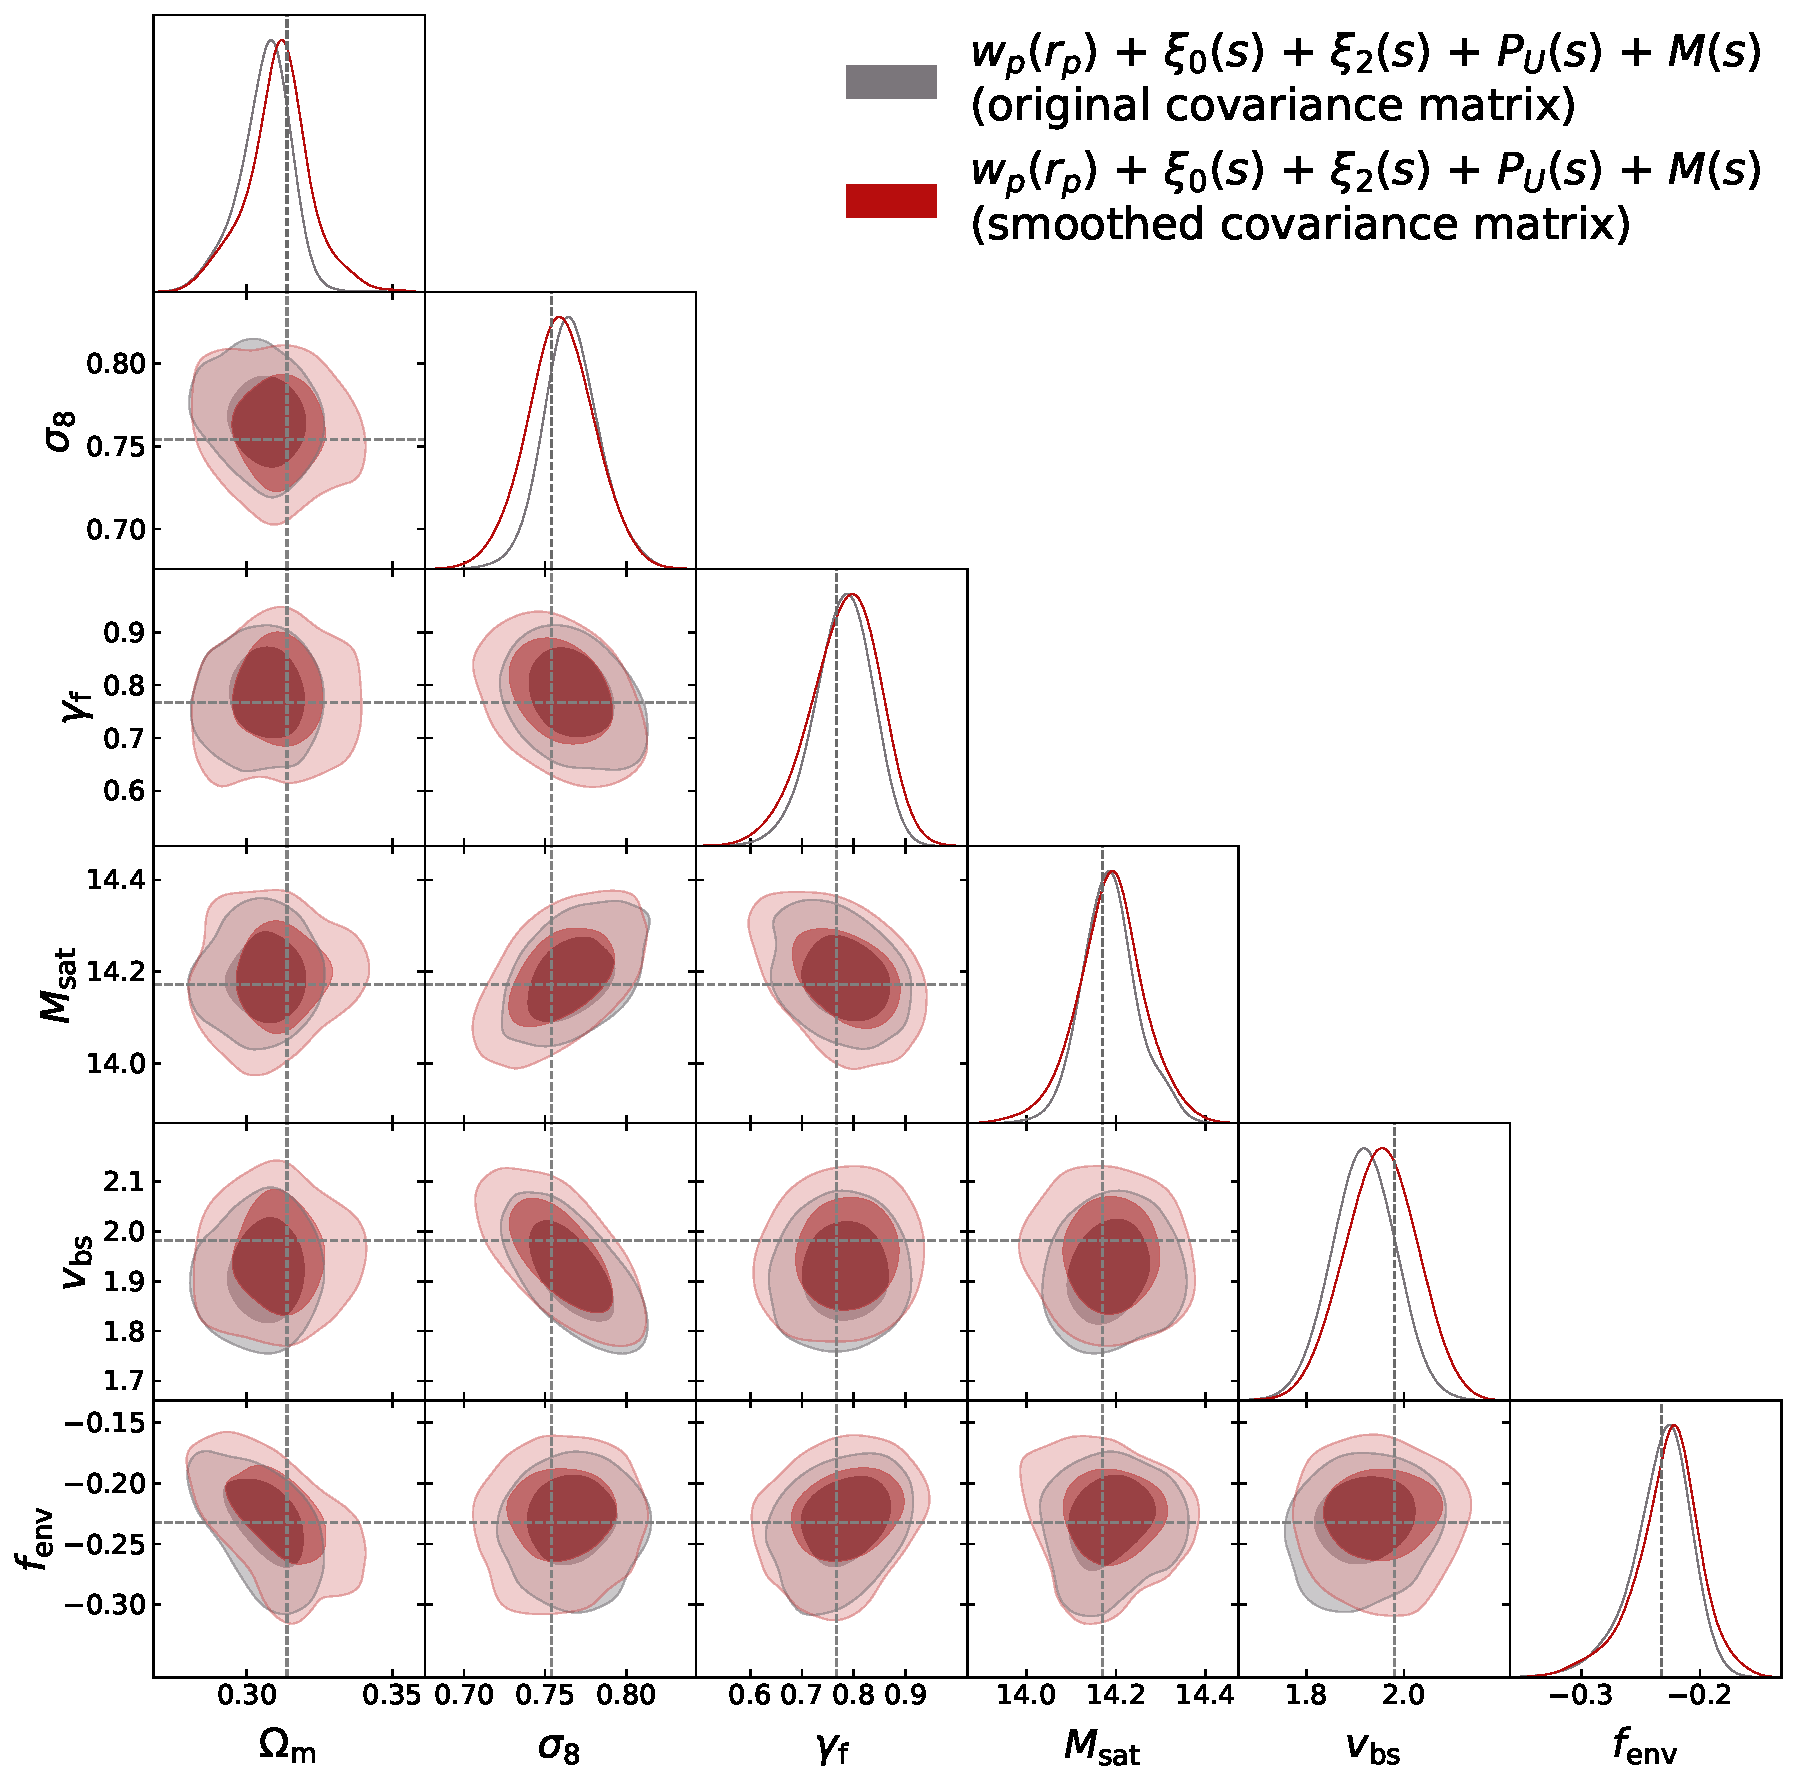
\includegraphics[width=0.47\textwidth]{contour_cov_c1h12}}
\hspace{1em}
\subfloat[\label{fig:contour_cov_c6h62}]{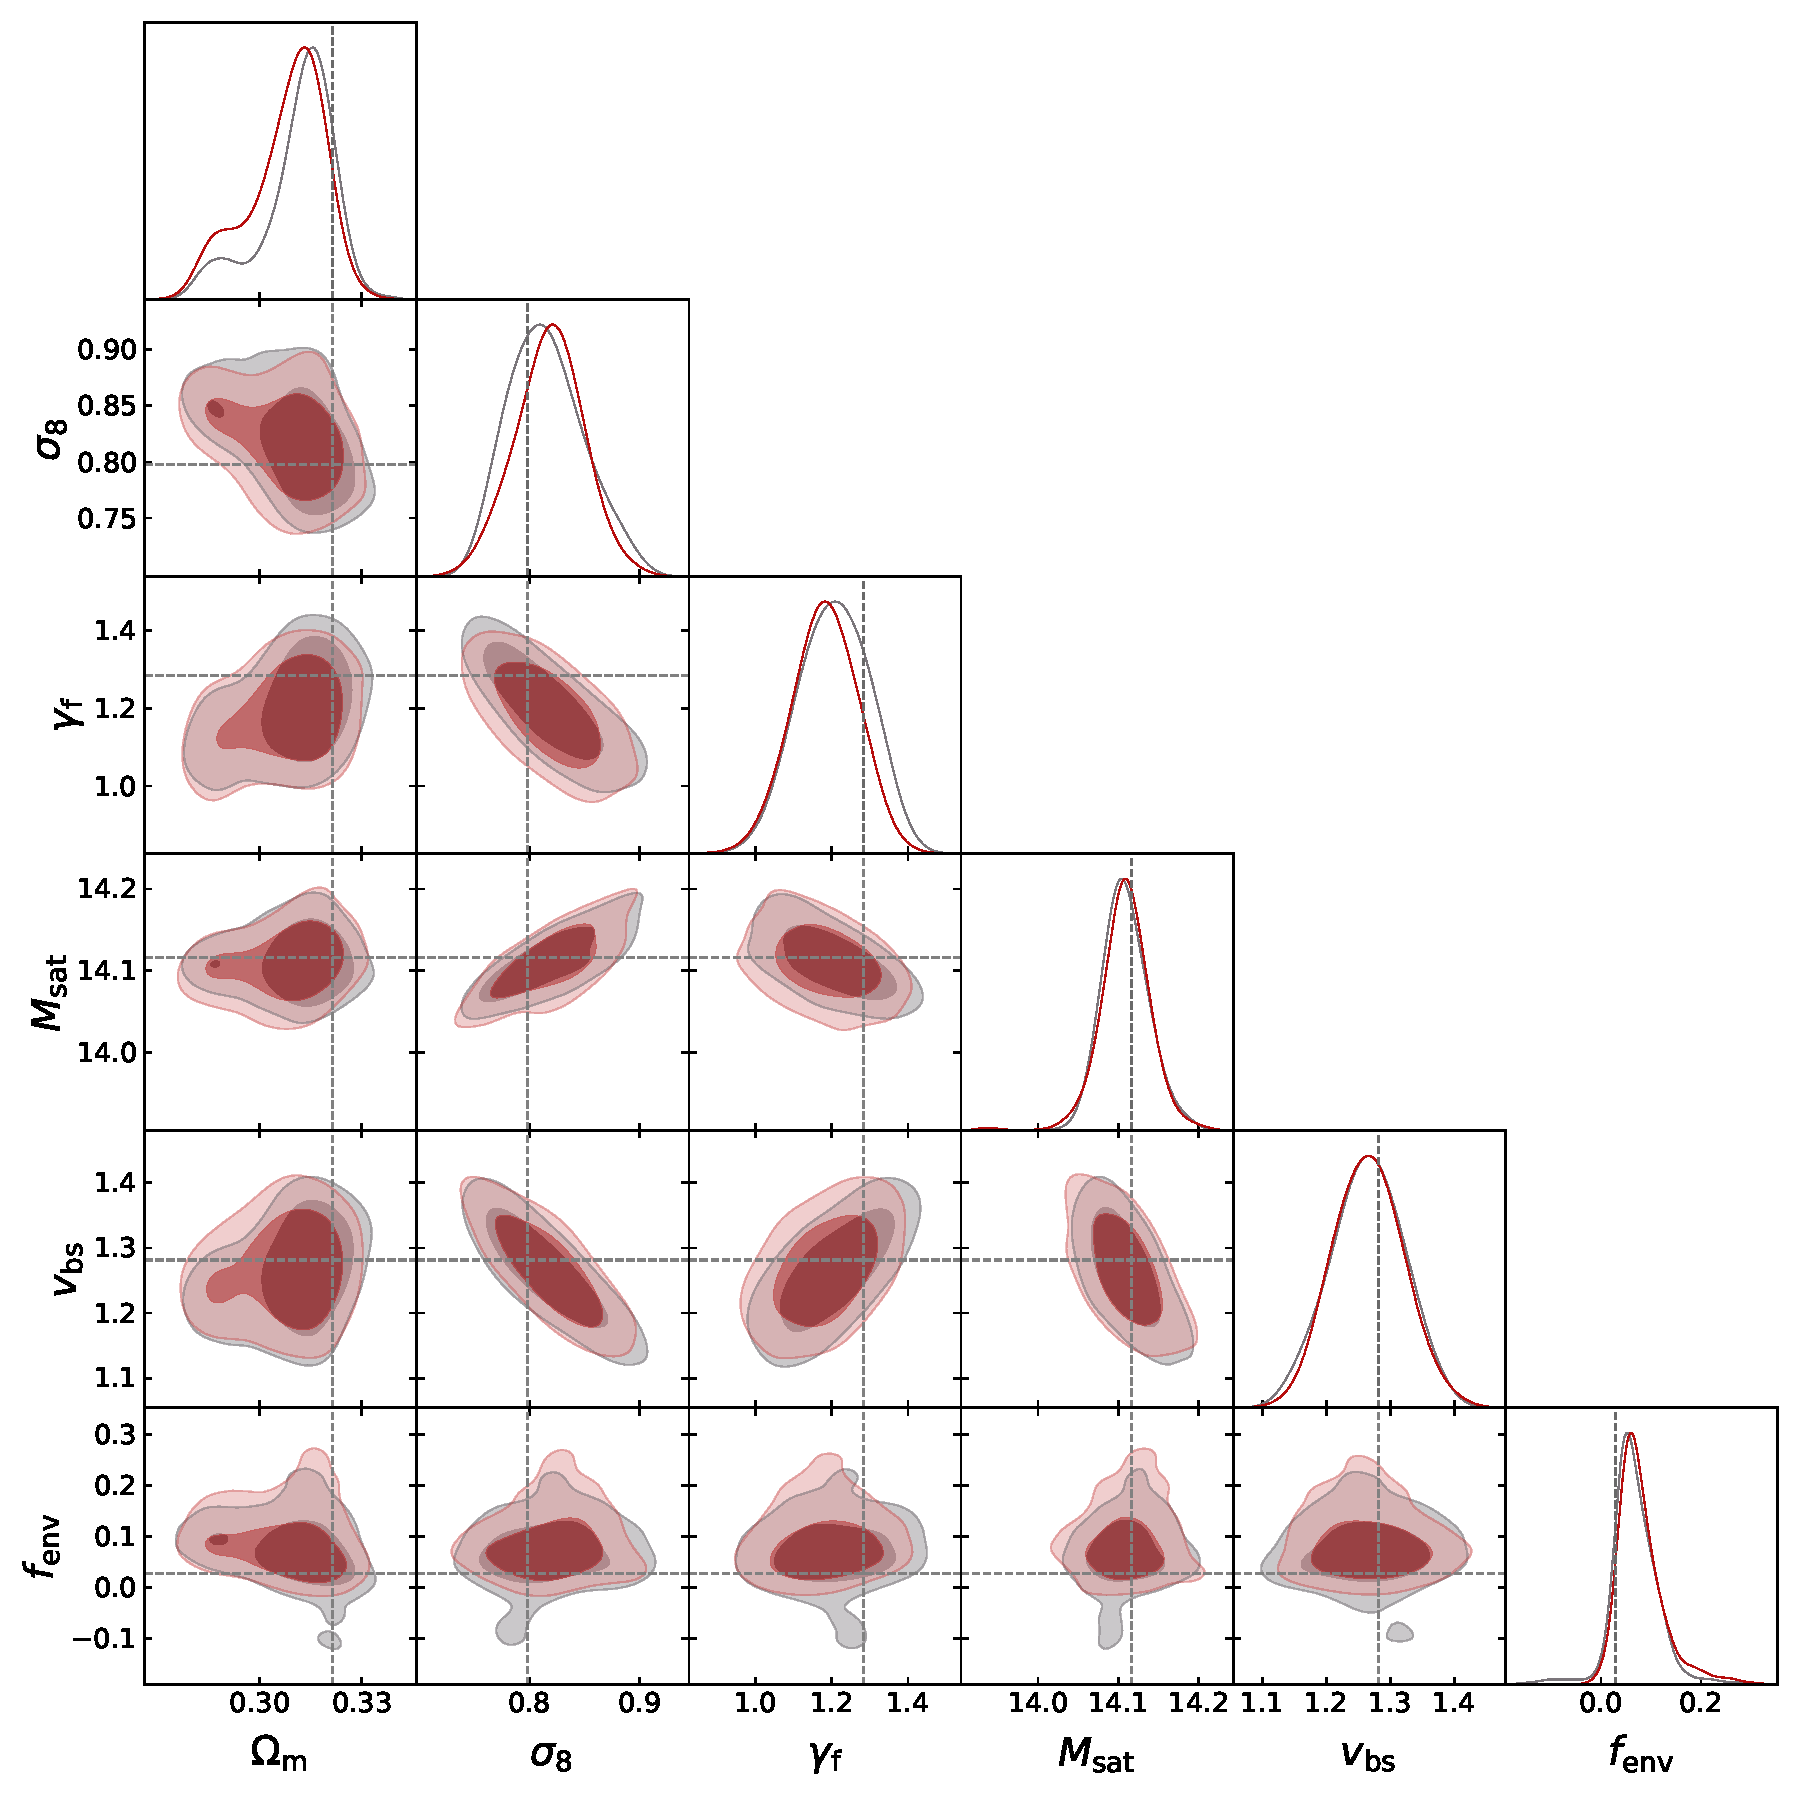
\includegraphics[width=0.47\textwidth]{contour_cov_c6h62}}
\caption{A comparison of the effect of the covariance matrix on recovered parameters. Panels (a) and (b) show recovery tests of key parameters for two different cosmology+HOD models, using all five observables, with the original covariance matrix compared to the covariance matrix with a Gaussian smoothing.}
\label{fig:contour_cov}
\end{figure*}

We compare the posteriors of recovery tests when using the original noisy covariance matrix compared with the Gaussian-smoothed covariance matrix, as described in \S\ref{sec:cov}.
The results are shown in Figure~\ref{fig:contour_cov} for two different cosmology+HOD models for a mix of key cosmological and HOD parameters.
We find that for the generally well-behaved model, Figure~\ref{fig:contour_cov_c1h12}, the posteriors are similar between the two covariance matrices, with the smoothed matrix resulting in slightly more accurate parameter estimates.
For the less well-behaved model, shown in  Figure~\ref{fig:contour_cov_c6h62}, the posteriors are quite noisy with the original covariance matrix.
Using the smoothed version cleans up some of the spurious modes in the posteriors, suggesting that the smoothing does help in avoiding issues related to noise in the covariance matrix. 
However, some of the modes persist even when using the smoothed matrix, indicating that perhaps we are still not properly sampling our parameter space, or that some of these regions of parameter space may be actual good fits to the observables and indicate true degeneracies in the parameters.


\subsection{Recovery test results for HOD \& assembly bias parameters}

\begin{figure*}[t]
\centering
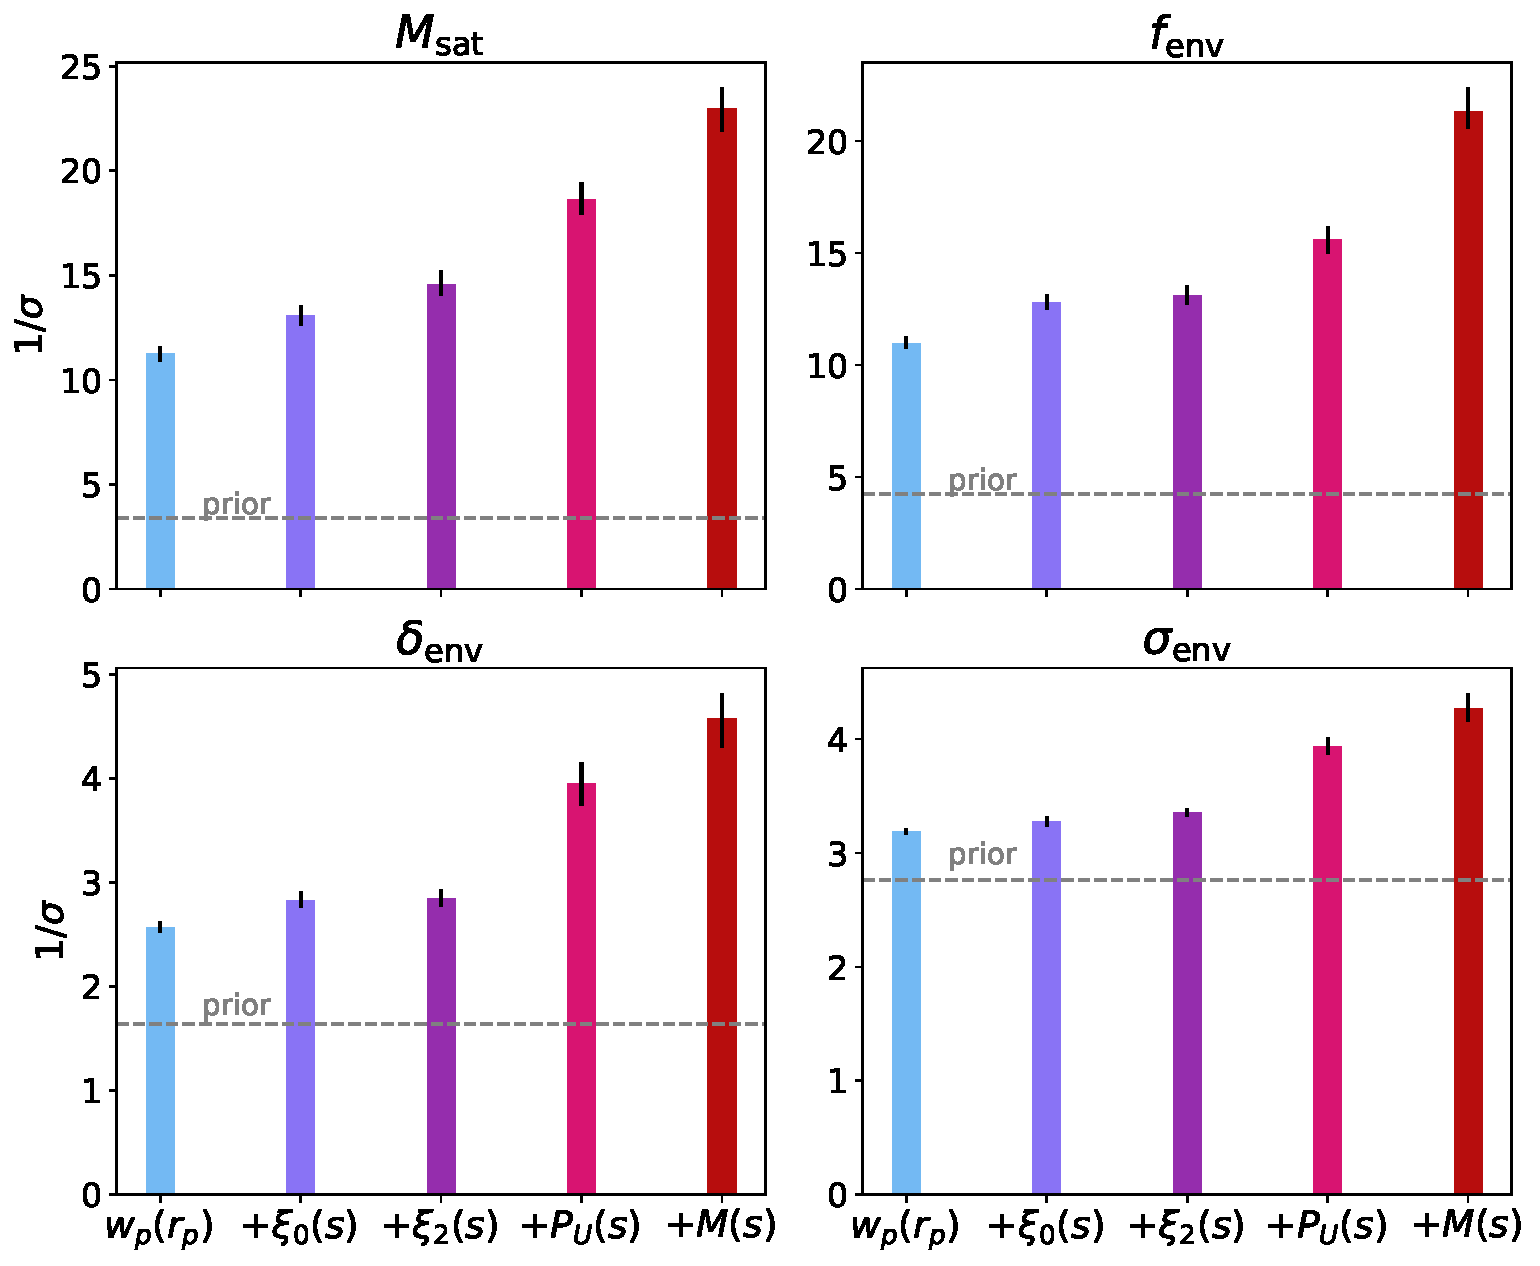
\includegraphics[width=0.6\textwidth]{recovery_hodab}
\caption{The precision of recovery tests when successively adding in observables, averaged over the 70 test models, for the HOD parameter $\msat$ and the three assembly bias parameters. Definitions are the same as in Figure~\ref{fig:recovery_single}.}
\label{fig:recovery_hodab}
\end{figure*}

We show the precision of our recovery tests for the HOD parameter $\msat$ and the three assembly bias parameters, $\fenv$, $\delta_\mathrm{env}$, and $\sigma_\mathrm{env}$, in Figure~\ref{fig:recovery_hodab}.
Results are shown averaged over the 70 test models, when successively adding in each of our five observables.
We see that for all of the parameters, each of the observables provides additional information on the parameter, with the exception of $\cfq$.
The two beyond-standard statistics $\upf$ and $\mcf$ provide significantly increased precision compared to the standard statistics alone.
This indicates that the additional constraining power from these statistics for the cosmological parameters may be related to their heightened sensitivity to assembly bias, and the ability of the combination of many observables to constrain the flexible HOD model.

It is somewhat surprising that $\wprp$ on its own provides significant constraining power over the prior on $\fenv$, the amplitude of environmental assembly bias.
Investigating the relationship between these, we find that with the rest of the parameters fixed, at large scales $\wprp$ decreases as $\fenv$ is increased. 
This makes sense as positive $\fenv$ values effectively transfer halos from high- to low- density regions, reducing overall clustering which translates to a lower two-halo term.
It is notable that this effect is significant enough to be able to constrain this parameter, and highlights the importance of including a flexible model of environmental assembly bias. 



\section{Discussion \& Conclusions}
\label{sec:discussion_aemulus}

We have constructed Gaussian process emulators for galaxy clustering statistics using the \aemulus simulation suite, including the non-standard statistics the underdensity probability function $\upf$ and the marked correlation function $\mcf$, which we expect to contain additional information relevant to constraining cosmological parameters of interest.
We achieve typical prediction errors of $\simo2\%$ with our emulator, depending on the scale and statistic, with a range of $<1\%-\simo10\%$.
Using held-out test simulations, we perform recovery tests to determine how well we can constrain the input parameters.
We find that including the beyond-standard statistics significantly increases the precision on the recovered parameters, by 33\% on 
$\sig$, 28\% on $\om$, and 18\% on $\gfs$.
We confirm that our framework is robust to different simulations and galaxy bias models by testing it on mock catalogs constructed from the Uchuu simulations and the SHAM method, on which we achieve unbiased constraints. 

To follow this proof-of-concept work, we will apply these emulators to measure the growth of structure in a current galaxy sample (BOSS or DESI). 
We expect that our combination of beyond-standard statistics with small-scale emulation will improve constraints; for instance, \cite{Satpathy2019a} used the marked correlation function to analyze the BOSS data and found that their results were limited by modeling RSD effects on small scales.
This analysis will require a careful treatment of many issues and subtleties in real data. 
We will have to handle redshift evolution, by working in redshift slices with emulators trained at the proper redshift.
We will require a sample constant in number density, both to match our emulators and because void- density-based statistics are particularly sensitive to variations in number density.
One of the main issues when applying to BOSS data will be fiber collisions, which lead to galaxies without measured redshifts, producing a nontrivial impact on clustering measurements especially at small scales (e.g. \citealt{Zehavi2002}).
Additionally, we will have to handle survey geometry effects including edges and bad fields.
The underdensity probability function and the local density-based marks used for the marked correlation will both be especially sensitive to these issues; we will apply fiber collision weights to the statistics and volume corrections to the spheres used for the density computations, and perform robust tests to ensure that we can recover unbiased parameters.

The application of this work to the BOSS sample will extend the project of \aemulus V \citep{Zhai2022}.
The \aemulus V analysis used $\wprp$, $\cfm$, and $\cfq$, the standard statistics discussed in this paper, and obtained tight constraints on the growth of structure parameter $\fsig$ in three redshift bins.
The analysis obtained a low value of $\fsig$ compared to Planck constraints based on a $\Lambda$CDM+GR model, adding to a recent wave of similarly low results based on small-scale clustering \citep{Chapman2021, Lange2022, Yuan2022}.
These studies are also based on standard clustering statistics; bringing in additional statistics and thus additional constraining power will allow for clearer tests of internal consistency between these analyses, as well as testing the demonstrated tension with Planck results.

There are multiple effects that could be contributing to this $\fsig$ tension.
One is additional baryonic effects that influence galaxy formation and are unmodeled in the HOD, introducing errors; while these are unlikely to be relevant at current precision, in future surveys they may become important.
Future work will incorporate additional flexibility in the galaxy bias and assembly bias models to test this hypothesis, and this will in turn require increased constraining power from the data.
The complementary information provided by non-standard statistics, as shown in this work, will be important in offsetting this flexibility to obtain high-precision constraints on $\fsig$ and help confirm or rule out this explanation for the $\fsig$ tension.
Another potentially relevant effect is that of massive neutrinos, which suppress the growth of structure in a scale-dependent way.
The next generation of the \aemulus simulations will incorporate massive neutrinos (The \aemulus Collaboration, in preparation), and the emulation of non-standard statistics will also be important in obtaining precise small-scale constraints from this updated model.

The effects of galaxy assembly bias are not yet a concern given the current precision of our surveys, as shown in the \cite{Zhai2022} BOSS RSD analysis, but as both our data and constraining power of methods improve, this will become a key source of uncertainty.
Previous works have found a small but significant dependence on halo environment (e.g. \citealt{Zehavi2018, Yuan2021}).
The density-sensitive statistics we investigate here, namely the $\mcf$ with marks as the galaxy number density on $10 \, \hMpc$ scales and the $\upf$ which measures underdense regions across a large range of scales, target this environmental bias.
The fact that incorporating these statistics improves our precision on recovering cosmological parameters suggests that galaxy occupation at fixed halo mass, and in turn galaxy clustering, does depend on the halo environment.
This is particularly clear when comparing the information in the $\mcf$ to the monopole $\cfm$, as these are similar statistics but with the former including local density information. 
We have shown that the density-sensitive statistics analyzed in this work are well-positioned to constrain environmental assembly bias and make precise cosmological parameter measurements.
Other sources of assembly bias, such as halo formation time, concentration, and spin, could be analyzed with marked correlation functions based on these properties, or other similarly targeted statistics; these can be readily incorporated into our emulation framework.

More broadly, this work confirms that additional clustering statistics can increase the constraining power in existing data with little added cost.
This approach could be extended to include other statistics that depend on the goals of the analysis.
These could include the three-point function (e.g. \citealt{TakadaJain2003, McBride2011}), the $k$NN-CDF \citep{Banerjee2021a}, and galaxy group statistics such as the group multiplicity function (e.g. \citealt{BerlindWeinberg2002}) and the group velocity dispersion.
We will explore some of these in future work.

One of the primary goals of the \aemulus project is to extract information from small-scale clustering, which is difficult to model theoretically and expensive to simulate fully.
Here, we have shown that there is significant information at small scales for nearly all of the statistics we analyze.
For the constraint on $\gfs$, we find that scales from $0.1 - 4 \, \hMpc$ contribute half of the information content, and that there is additional information all the way down to $0.1 \, \hMpc$
This confirms a similar result by \cite{Zhai2019}, which uses $\wprp$, $\cfm$, and $\cfq$, and includes the halo velocity field scaling parameter $\gf$. 
Some recent analyses have not found as much additional information at these small scales.
\cite{Lange2022} concludes that for their low-redshift sample, which is closer in number density to the one analyzed here, scales between $1-2 \hMpc$ increase the constraining power on $\fsig$ by a small amount, and scales below $\simo1 \hMpc$ not at all.
As discussed in \S\ref{sec:scaledep}, they do not incorporate a $\gf$ parameter to scale the velocity field, and they do not use $\wprp$ as we do.
This model flexibility, which \cite{Zhai2019} also includes, combined with that statistic sensitive to velocity information, may allow us to extract additional information from small scales.
The analysis by \cite{Lange2022} does include an assembly bias model using the decorated HOD framework \cite{Hearin2016}, but this is not as flexible as our three-parameter environmental assembly bias model.
Our increased flexibility on this front may also contribute to the discrepancy, though future work should revisit these hypotheses.

Finally, in this work we built emulators at fixed redshift and scale.
To apply to different data sets, we will require predictions at various redshifts, for which suites of emulators can be constructed and trained at the needed redshifts; an extension of this work could construct emulators that are able to make predictions as a continuous function of redshift.
In a similar vein, here we emulated the clustering statistics at fixed scale, with a different model trained for each bin. 
In future work, we could train the model on all bins simultaneously to include the full covariance properties; even better, we could include scale as an input parameter and make predictions at any scale.


\section*{}
 
\textit{Software:} numpy \citep{VanDerWalt2011}, IPython \citep{Perez2007}, scipy \citep{Virtanen2020}, matplotlib \citep{Hunter2007}, corrfunc \citep{SinhaGarrison2019, Sinha2020}, halotools \citep{Hearin2017}, dynesty \citep{Speagle2020}, george \citep{Ambikasaran2016}, getdist \citep{Lewis2019}.
Our emulator and related data products are publicly accessible at \url{https://github.com/kstoreyf/aemulator}.

\section{Chapter Acknowledgements}

K.S.F. thanks Sean McLaughlin, Johannes Lange, Sihan Yuan, David W. Hogg, and the Astronomical Data group at the Center for Computational Astrophysics for helpful discussions.
This work received support from the U.S. Department of Energy under contract number DE-AC02-76SF00515 and from the Kavli Institute for Particle Astrophysics and Cosmology.
K.S.F. is supported by the NASA FINESST program under award number 80NSSC20K1545.
J.L.T. acknowledges support of NSF grant AST-2009291.
J.D.~is supported by the Lawrence Berkeley National Laboratory Chamberlain Fellowship.
This research made use of computational resources at SLAC National Accelerator Laboratory and the NYU Department of Physics; authors thank the SLAC computational team and Mulin Ding at NYU for computational support.
This research used resources of the National Energy Research scientific Computing Center, a DOE Office of Science User Facility supported by the Office of Science of the U.S. Department of Energy under Contract No. DE-AC0205CH11231.




\chapter{Characterizing Dark Matter Halos using Exact Physical Symmetries}
\setcounter{section}{-1}
\label{chp-eqcosmo}
This chapter is based on work in collaboration with David W. Hogg, Shy Genel, and Soledad Villar.

\graphicspath{{figures/figures_eqcosmo/}}


\section{Chapter Abstract}
The laws of physics obey exact symmetry properties.
The method of invariant scalars is a lightweight and physically motivated way to encode these symmetries in analysis methods, by compressing inputs into scalars that are invariant to rotations, translations, and permutations (particle labeling).
We apply this approach to analyze the relationship between dark matter (DM) and baryons in cosmological simulations, which is critical for understanding the galaxy--halo connection and inferring cosmological parameters from large-scale structure.
Using IllustrisTNG simulation data, we build a training set consisting of DM halos in the DM-only simulation and their corresponding central galaxies in the matched hydrodynamical simulation. 
For each DM halo, we construct a large set of invariant scalars based on geometric phase-space properties of the DM particle distribution.
With these scalars as inputs, we use a neural network to predict the properties of the corresponding galaxies, most importantly the stellar mass.
We show that our approach outperforms the use of standard halo summary properties as the features, as well as using the same geometric information but not compressed into invariant quantities.
The exact symmetries inherent to our method impose informative constraints while preserving the known invariance properties of large-scale structure.
Further, our results are interpretable in terms of the information in DM phase-space and give insight into the connection between galaxy and DM halo properties, relevant to open questions in galaxy formation including the importance of assembly bias on the galaxy--halo connection.


\section{Introduction}

Overdense regions of dark matter (DM) in the universe collapse to form DM ``halos'', which merge and grow to form the underlying structure of the cosmic web (e.g. \citealt{davis_evolution_1985,bond_how_1996,boylan-kolchin_resolving_2009}). 
These DM halos play host to the galaxies that populate our universe, and DM evolution and galaxy formation are deeply intertwined. 
The merger history of halos affects how their galaxies develop, and galactic feedback can in turn affect the growth of structure.
This relationship, known as the galaxy--halo connection \citep{WechslerTinker2018}, is core to both galaxy formation and large-scale structure.

Cosmological hydrodynamic simulations have become extremely powerful tools to model the formation of structure and galaxies (e.g. \citealt{springel_gadget_2001, genel_introducing_2014,dave_simba_2019}).
However, they are very computationally expensive, consuming millions of CPU-hours; even their DM-only counterparts are relatively expensive.
Recently, there have been efforts to \emph{emulate} these cosmological simulations with faster tools, such as machine learning (ML) techniques.
These offer the opportunity to both help us understand the key physical processes affecting structure galaxy formation, as well as construct the large number of mock galaxy catalogs needed to analyze current galaxy surveys. 

There is a growing body of work on learning the relationship between dark matter and galaxy properties using ML-based approaches.
Many of these use a small set of properties of identified DM halos as input features, and focus on predicting the galaxy stellar mass as well as other baryonic properties.
\cite{jo_machine-assisted_2019} show that using extremely randomized trees (ERTs) and including a two-stage learning approach and environmental property features produce accurate galaxy property predictions in the IllustrisTNG simulation.
\cite{lovell_machine_2021} use ERTs to learn the relationship between halos in the EAGLE simulation and galaxies in the zoom C-EAGLE simulations of galaxy clusters.
\cite{de_santi_mimicking_2021} compare the performance of different ML models on predicting galaxy properties from IllustrisTNG, and find success in predicting the stellar mass and reproducing galaxy power spectra.
\cite{delgado_modeling_2021} use a random forest regressor to identify key secondary halo properties for modelling the galaxy--halo connection using IllustrisTNG.
\cite{stiskalek_scatter_2022} also explore how secondary halo properties affect the galaxy--halo connection, specifically analyzing the scatter in the stellar-to-halo mass relation in IllustrisTNG using a neural network ensemble.   
\cite{jespersen_learning_2022} use graph neural networks on DM halo merger trees of halos in the DM-only IllustrisTNG simulation to predict galaxy properties computed from semi-analytic models.

Other works use the dark matter density field as inputs, rather than halo features.
This approach operates on inputs closer to the raw data, but presents its own challenges such as the high sparsity in the stellar mass distribution.
\cite{yip_dark_2019} implement a cascade of convolutional neural networks (CNNs) to predict the 3D galaxy distribution from a voxelization of the IllustrisTNG DM-only simulation.
Along a similar vein, \cite{kasmanoff_dm2gal_2020} predict the stellar mass in voxels centered on subhalos using CNNs in IllustrisTNG.

Another line of inquiry seeks to use ML to emulate and understand structure formation in the dark sector.
Many works have explored using neural networks to map the initial displacement field of a particle grid as to the final displacement field, targeting a full or approximate N-body simulation \citep{he_learning_2018,jamieson_field_2022}.
Others aim to map the final displacements from a very inexpensive N-body simulation substitute to a more realistic output \citep{piras_fast_2023}. 
To develop a deeper understanding of structure formation, \cite{lucie-smith_insights_2022} use gradient-boosted trees to predict late-time mass profiles of DM halos based on input initial conditions and elucidate the relevant scales at play.
\cite{etezad-razavi_unravelling_2023} investigate the role of the velocity field on DM halo masses using CNNs.

While ML techniques are extremely powerful at making predictions, they are generally agnostic to the underlying physical processes they model.
One key aspect of physical laws is \emph{symmetries}: we expect that our results will change in exact ways, or not change at all, under certain transformations.
Some ML models are naturally \emph{equivariant} to certain symmetries, such as convolutional neural networks to translations and graph neural networks to permutations.
Recently, additional ML approaches that enforce physical symmetries have been developed.
CNNs have been extended to incorporate rotational symmetries \citep{cohen2019gauge,wang2021incorporating,ocampo_scalable_2023}.
Most relevant to our focus on simulated dark matter halos,neural networks that operate on point clouds have been developed that enforce rotation, translation, and permutation equivariance using a variety of approaches.
These include irreducible representations \citep{thomas2018tensor}, self-attention mechanisms \citep{fuchs2020se}, and convolutions \citep{kondor2018covariant,zhang2019rotation}, as well as extensions of graph neural networks \cite{Satorras2021}.

Approaches to learning the galaxy--halo connection that are based on a set of halo properties are often naturally obey obey the relevant symmetries; for instance, mass and concentration are invariant to rotations, translations, and permutations of the DM halo particles.
On the other hand, ML models operating directly on the dark matter density field do not typically respect all of these symmetries.
Recent work has applied explicitly equivariant neural network architectures and approaches to structure formation and the galaxy--halo connection in cosmological simulations.
\cite{dai_learning_2020} use Lagrangian Deep Learning to reproduce both dark matter evolution and hydrodynamical outputs, based on an initial linear density field; this approach respects translational and rotational symmetries.
\cite{thiele_predicting_2022} use permutation- and rotation-invariant DeepSets to predict the thermal Sunyaev-Zel'dovich field in galaxy clusters in IllustrisTNG.

In this work, we propose an equivariant approach to characterizing the dark matter distribution that enforces the known symmetries of cosmological simulations. 
We use the method of \emph{invariant scalars} introduced by \cite{Villar2021a}, which offers a lightweight approach to representing invariant and equivariant functions using a collection of scalar quantities.
The core idea is that geometric objects---such as vectors of particle positions and velocities---can be \emph{contracted} to form scalars that are invariant to transformations, namely translations, rotations, velocity boosts, and permutations.

Recent work has shown that this ``scalars'' approach improves performance on prediction tasks.
\cite{yao_simple_2021} demonstrated the approach on a toy dynamical system and showed that it outperformed state-of-the-art approaches in both speed and accuracy.
It has recently been applied to large-scale structure problems: \cite{villanueva-domingo_learning_2022} used scalars in combination with graph neural networks applied to simulated galaxy catalogs to perform cosmological inference.
\cite{thiele_predicting_2022} constructed invariant scalars from input dark matter particles as well as galaxy cluster-scale features as inputs to their DeepSet architecture.

We apply the invariant scalars approach to the particle distribution of DM halos in the IllustrisTNG DM-only simulation.
To obtain a uniform set of features across halos while preserving detailed structure, we first compress the DM halo particles into geometric multipole moments in radial bins, and then combine these into invariant scalar features.
This provides a characterization of DM halos that encodes interpretable, high-order phase-space structure while preserving physical symmetries.
To learn the mapping from DM halos to baryonic properties, we construct a set of matched DM halos in the DM-only simulation to central galaxies in the TNG hydrodynamical simulation.
We use a XXX model with the scalars as inputs to predict galaxy properties, and compare this approach to benchmark feature sets. 
We also demonstrate that these features allow for accurate predictions of the mass assembly history of the DM halos.

In this work, we use the following notation: 
Scalars are denoted by lowercase variables, vectors by lowercase bold variables, and tensors by uppercase variables.

This paper is outlined as follows.
In \S\ref{sec:sim_sample}, we introduce the simulation used and our halo and galaxy sample selection. 
We discuss our approach to constructing invariant scalars from dark matter halo particle distributions in \S\ref{sec:scalars_approach} 
In \S\ref{sec:features_model}, we detail the fiducial scalar feature set and other benchmark feature sets we use as inputs, and describe the prediction model.
In \S\ref{sec:results}, we present the results of predicting the mass assembly history and galaxy properties from DM halo features, and in \S\ref{sec:discussion}, we interpret these results and discuss their implications and applications.
We summarize our results and conclusions in \S\ref{sec:summary}.


\section{Simulation and Sample Construction}
\label{sec:sim_sample}

\subsection{The IllustrisTNG simulations}
\label{sec:sim}

The Illustris TNG simulations are cosmological magnetohydrodynamical simulations that co-evolve dark matter and baryons to model galaxy formation \citep{springel_first_2018,nelson_first_2018,pillepich_first_2018,naiman_first_2018,marinacci_first_2018}.\footnote{Data products from the TNG Project are publicly accessible at \url{https://www.tng-project.org/}.}
The simulations are run starting from initial conditions at $z=127$ with cosmological parameters from \cite{ade_planck_2016} $\Omega_m = \Omega_{dm} + \Omega_b = 0.3089$, $\Omega_b = 0.0486$, $\Omega_\Lambda = 0.6911$, Hubble constant $H_0 = 100$ $h$ km s$\inv$ Mpc$\inv$ with $h = 0.6774$, $\sigma_8 = 0.8159$, and $n_s = 0.9667$.
They model baryonic processes including ionizing background radiation, star formation and stellar feedback, stellar evolution and chemical enrichment, pressurization of the interstellar medium from supernovae, and the growth of and feedback from supermassive black holes.   
We use the TNG-100-1 simulation, which has a size of $L = (75 \hMpc)^3$, $1820^3$ DM particles and the same number of gas cells, and mass resolutions of $m_\text{DM} = 7.5 \times 10^6 \Msun$ and $m_\text{gas} = 1.4 \times 10^6 \Msun$.
The simuluation also evolves star/wind and black hole particles.
It has a matched DM-only simulation run with the same initial conditions, TNG-100-1-Dark, with mass resolution of $8.9 \times 10^6 \Msun$.
We refer to the DM-only simulation (TNG100-1-Dark) as \dark and the hydrodynamical simulation (TNG100-1) as \hydro in the rest of this work.
For most of this work, unless otherwise stated, we use the $z=0$ snapshot.

We use the DM halo catalogs provided by the TNG project as the starting point for our sample.
Halos are defined by a Friends-of-Friends (FoF) algorithm on DM particles, with a linking length of 0.2 times the mean inter-particle separation; other types of particles are assigned to the same halo as their nearest DM particle.
Subhalos within halos are found using the Subfind algorithm, which identifies gravitationally bound structures across all particle types.


\subsection{Halo and galaxy sample selection}
\label{sec:select}

One of our goals with this project is to propose a characterization of DM halos that is useful for predicting the properties of the galaxies they host, as well as their assembly history.
Given this, we operate on the halos in the \dark (DM-only) simulations, with the idea of learning the results of the hydrodynamic galaxy formation model.
To that end, we construct a sample of paired DM halos in the \dark simulation and galaxies in the \hydro (full hydrodynamical) simulation. 
We consider only central galaxies in this work; the approach could be straightforwardly extended to satellite galaxies.

We first make a cut on the \dark halos, choosing only halos with a mass $\Mfof > 10^{10.25} \, \hMsun$, where $\Mfof$ is the mass of all the particles that are part of the FoF group within $\Rtwoh$, and $\Rtwoh$ is the radius enclosing a mass of 200 times the mean density of the simulation.
We use this mass definition, as opposed to the typical $\Mtwoh$ which includes all particles both part of and not part of the FoF group, as our approach will operate only on the FoF particles and this keeps the mass definitons consistent; however, this is just for technical reasons, and only differs at the few percent level.
We require that the halos have at least one subhalo.
We use the matched subhalo catalogs provided by the TNG Project, which match subhalos in the dark simulation to subhalos in the paired hydrodynamical simulation; we call these subhalo pairs ``twins''.
The matching is done with the ``LHaloTree'' algorithm, which selects the halo in the other simulation with the largest number of DM particles in common, and requires that both simulations agree, resulting in bijective matches.
We discard halos that do not have a \hydro match.
For every \dark halo, we take its most massive \dark subhalo.
For that \dark subhalo, we find its twin \hydro subhalo.
We consider the baryons in this subhalo to constitute the central galaxy that is associated with the original \dark halo; we call this the ``matched'' galaxy of the \dark halo. 
We note that this twin \hydro subhalo is nearly always (but occasionally not) the most massive subhalo in its parent halo in the \hydro simulation.

We make some additional cuts on this sample.
We note that some of these cuts are on the ``labels'' or otherwise require knowledge of the hydrodynamical simulation; in a full application this should be handled more carefully, such as implementing an additional prediction step. 
We discard all \dark halos for which the twin \hydro subhalo has fewer than 50 star particles.
We discard all pairs for which the mass $\Mtwoh$ of the DM halo and the matched hydro halo differ by a factor of 3 or more; we assume that this indicates a bad match, and only occurs for a very small fraction of halos.
We also require that the SC-SAM has been applied to the halos, as we use the halo assembly histories computed by the SC-SAM (discussed further in \S\ref{sec:mah}); this removes a few percent of the halos.
These selections result in XXX \dark halos and matched \hydro galaxies.
We use 70\% as a training set, 15\% as a validation set, and 15\% as a test set.


\subsection{Halo mass assembly history}
\label{sec:mah}

We aim to predict the mass assembly history of the \dark halos based only on their present-day ($z=0$) properties.
This is informative as it captures the dynamical history of the halo, which affects the formation of the galaxies it hosts.
We use the merger histories computed by \citep{gabrielpillai_galaxy_2021} as part of a comparative analysis between TNG and the Santa Cruz semi-analytic model (SC-SAM, \citealt{somerville_semi-analytic_1999,somerville_semi-analytic_2008, somerville_star_2015}); the SAM is based on these merger trees.\footnote{The merger history and other SC-SAM data is publicly accessible at \url{https://github.com/aust427/illustris_sam}.}
The merger trees are run on halos found with the \textsc{rockstar} \citep{behroozi_rockstar_2013} code and built with \textsc{consistent trees} \citep{behroozi_gravitationally_2012}, and a bijective matching is performed between the \textsc{rockstar} and TNG Subfind halos.

We consider the most massive progenitor branch of the assembly history of each \dark halo in our sample.
We compile the mass of the halo's most massive progenitor for each of the TNG snapshots. 
A natural quantity to try to predict would be the mass of the most massive progenitor halo as a function of redshift; this could be made dimensionless  by considering the fraction of mass accreted by the halo's most massive progenitor compared to its $z=0$ mass.
However, different halos can be traced back to different redshifts, and this inconsistency causes difficulties at the prediction stage.
We thus choose to learn the scale factor $a$ (related to the redshift $z$ by $a=1/(1+z)$) at which the halo has accreted a given fraction of its mass along the most massive progenitor branch, $M_\mathrm{vir}(a)$/$M_\mathrm{vir}(a=1)$, where $M_\mathrm{vir}$ is given by the \field{HalopropMvir} field (equivalent to the TNG field \field{Group\_M\_TopHat200}) of the SC-SAM data and $a=1$ is the present day.
(We note that this is a different mass definition than that used throughout this work, but we only consider mass ratios so we expect this will not matter.)
This swapped quantity, the scale factor $a$ as a function of mass fraction, gets at the same information as the natural quantity but is more stable in predictions.
We compute this at mass fractions linearly spaced by 0.025 between 0 and 1 (exclusive), giving 39 values. 
As we only have the history at a finite number of snapshots, we perform a linear interpolation between the mass fractions and scale factors to estimate the scale factor at a given mass fraction.
If the target mass fraction is outside the bounds of the data (for example, if the initial mass of the halo was a larger mass fraction than our tabulated values), we assign the scale factor to be that at which the mass fraction is closest.



\subsection{Baryonic properties and uncertainties}
\label{sec:galprops}

% TODO: add uncertainty info here
One of the aims of this work is to predict the baryonic properties of central galaxies hosted by a given dark matter halo.
In this section we detail these properties and the associated choices we make. 
We choose to predict only scalar properties for this work, as we focus on enforcing \emph{invariance} to physical symmetries, though we could also predict vector and higher order properties and enforce \emph{equivaraince}.

The primary target is the galaxy stellar mass $\mstellar$, the mass of all of the star particles belonging to the twin \hydro subhalo of the \dark halo.
We use the TNG field \field{SubhaloMassType} for star particles, and convert to units of log($\hMsun$).
Stellar mass is the main quantity used for creating mock catalogs, and is tightly coupled to nearly all other galaxy properties, so we focus on this quantity in this work.
We also aim to predict the following other baryonic properties: 
the stellar half-mass radius $\rstellar$, the specific star formation rate averaged over 1 Gyr $\ssfr$, the specific stellar angular momentum $\jstellar$, the black hole mass $\mbh$, and the color $\gminusi$. 
The stellar radius $\rstellar$ is the TNG property \field{SubhaloHalfmassRadType} of the subhalo for star particles, in units of log(kpc/$h$).
The value of $\ssfr$ is based on the star formation rate catalogs provided by the TNG Project \citep{donnari_star-formation_2019,pillepich_first_2019}.
We use the \field{SFR\_MsunPerYrs\_in\_all\_1000Myrs} field, the star formation rate including all bound star particles of the subahlo, and take the ratio with the stellar mass $\mstellar$; we use units of log(yr$\inv$).
For the galaxies that have $\ssfr=0$, we assign a small value based on the average gas mass cell and the 1 Gyr timescale ($\text{SFR}_\mathrm{zero} = 10^{-3} \hMsun \text{yr}\inv$).
We use the $\jstellar$ computed by the approach of \cite{genel_galactic_2015} in the same way as the \field{SpecificAngMom} field in the TNG Project catalog, with units km s$\inv$ kpc. 
The $\mbh$ value is that given by the TNG field \field{SubhaloBHMass} of the subhalo, in units of log($\hMsun$).
For galaxies with zero black hole mass, we assign the value to be half of the minimum black hole mass in our sample. 
We use the $g-i$ color comptuted from synthetic SDSS photometry as provided by the TNG project \citep{nelson_first_2018}; the photometry is in units of AB magnitudes. 
The distributions of these properties as a function of \dark halo mass are shown in the left column of Figure~\ref{fig:galprops}.

We estimate the uncertainties on these baryonic properties based on the effects of small initial perturbations in cosmological simulations and how these propogate to differences in baryonic properties over time.
We quantify this using the simulations of \cite{Genel2019}, which are pairs of IllustrisTNG with small random initial particle displacements.
The $z=0$ galaxies are then matched across the pairs, and the pairwise differences between their properties can be computed; the standard deviations of these pairwise differences represent a lower limit on the retrievable information on the properties.
We refer to this as the chaotic limit, and use it as a comparison for our baryonic property predictions.
Specifically, we use the $\epsilon=1$ resolution level simulations which is similar to but slightly worse than the resolution of TNG100-1, so the limit is slightly optimistic (the true lower limit is actually lower than the limit shown).


\section{The invariant scalars approach}
\label{sec:scalars_approach}

Our method for characterizing DM halos is based on the ``scalars'' approach of \cite{Villar2021a}.
The core idea is that functions invariant or equivariant to certain transformations can be expressed in terms of a set of scalars, constructed from the input quantities.  
This is motivated by the fact that the physical laws that govern the evolution of the universe---and thus cosmological simulations---obey exact classical symmetries.
We outline our approach here to apply the scalars approach to DM halo characterization and prediction tasks, and go into further detail in the rest of this section.

Our goal is to characterize DM halos in a way that captures detailed phase-space structure while enforcing invariance to transformations.
(The same approach applies to equivariance, but here we aim to predict scalar properties and thus focus on invariance.)
We specifically consider rotation, translation, velocity boosts, rotation, and permutation (of the particles); these are detailed in \S\ref{sec:symmetries}.
For each \dark halo, we use a multipole expansion to compress the particle positions and velocities of each halo into a set of ``geometric features'' that describe the phase-space structure of the halo; this is discussed in \S\ref{sec:geometric_features}.
We then construct scalar contractions of these geometric features, which are scalars, vectors, and tensors; these ``scalar features'' are invariant to transformations of the particles. 
This step is informed by Einstein summation notation, which only allows invariant scalars to be produced; the details of our scalar feature construction is discussed in \S\ref{sec:scalar_features}.
We can finally use these scalar features as the inputs for our prediction task; in our case we use a Gradient Boosted Tree model (\S\ref{sec:prediction_model}), though we note that the scalars could be used with other model choices.

In contrast to this approach, many standard approaches use a small set of hand-constructed properties of the halos, such as the mass, concentration, and spin.
While these do often obey physical symmetries, this is not enforced; further, the properties are hand-picked and can be non-trivial to compute, and they do not necessarily capture the complexity of the phase-space structure of the halos.
We use these ``standard features'' as a benchmark, detailed in \S\ref{sec:benchmarks}.
Other approaches work on the full particle distribution, or the smoothed density field; while this captures the detailed halo structure, it does not obey many of the physical symmetries (depending on implementation), and can be very expensive.
The scalars approach captures the benefits of both of these standard approaches: it allows for a flexible, lightweight set of halo features that respects symmetries and provides a more complete representation of DM structure.
\ksf{move this to discussion?}
We also expect the enforced equivariance to make the approach more generalizable, for instance to different resolutions or simulation codes.


\subsection{The physical symmetries}
\label{sec:symmetries}

% to write
%what is a geometric object? scalars, vectors, tensors - defined by their transformation properties under rotation, translation, permutation. properties that ensure that coordinate freedom preserve angular momentum, linear momentum, etc

\subsection{Geometric features}
\label{sec:geometric_features}

\begin{table}
    \caption{The geometric features we construct from the \dark halo particles, following the multipole expansion of \eqt{eq:geo}. The table gives for each feature its name in multipole moment and more readable notation, its order (rank), and its degree in mass, position, and velocity, and its physical interpretation. All of the geometric features have mass degree of 1 as the are constructed as single sums over masses.}
    \label{tab:geos}
    \vspace{0.5em}
    \centering
    \begin{tabular}{|l|l|l|l|l|l|l|}
    \hline
    moment & name & order & $m$ deg. & $\x$ deg. & $\vel$ deg. & physical interpretation \\
    \hline
    $g_{00n}$ & $m_n$ & 0 & 1 & 0 & 0 & mass in $n$th bin \\
    $g_{10n}$ & $\x_n$ & 1 & 1 & 1 & 0 & mass-weighted position of $n$th bin \\
    $g_{01n}$ & $\vel_n$ & 1 & 1 & 0 & 1 & mass-weighted velocity of $n$th bin \\
    $g_{20n}$ & $\Cxx_n$ & 2 & 1 & 2 & 0 & variance tensor of positions in $n$th bin \\
    $g_{11n}$ & $C^{(\x\vel)}_n$ & 2 & 1 & 1 & 1 & covariance of pos. and vels. in $n$th bin \\
    $g_{02n}$ & $\Cvv_n$ & 2 & 1 & 0 & 2 & variance tensor of velocities in $n$th bin \\
    \hline
    \end{tabular}
\end{table}

We first compute a set of \emph{geometric features} from our data from the particle distribution, specifically their masses, positions, and velocities. 
There are multiple reasons we do this.
Theoretically we could compute scalars directly from the particles that consitute the halo; in fact, this would be simpler as these are all scalars and vector inputs.
However, this results in an enormous number of scalars as it would require the inner product of each pair of particles, scaling as the square of the number of particles.
It also would produce a different number of particles for each halo, which is difficult to handle at the prediction stage.
Finally, the ordering of the scalars is not clear and the permutation invariance would be brittle at best.
By first condensing the particles into a uniform set of geometric features, we circumvent all of these issues.
We note that there are many ways to handle this step, and we have chosen one relatively simple option.

We choose the geometric features to be based on a multipole expansion, computing moments of the data in a set of radial shells. 
We define the geometric features $g_{\ell p n}$ as: 
\label{eq:geo}
\begin{equation}
    g_{\ell p n} = \sum_i m_i \, W_n(r_i) \, \left( \x_i^{\otimes \ell} \, \otimes \, \vel_i^{\otimes p} \right)
\end{equation}
where $i$ indexes the particle, $m_i$ is the mass of the $i$th particle, $W_n(r_i)$ is the $n$th window function (defining the radial bins), and $r_i$ is the distance between the position of the $i$th particle and some fiducial point.
% TODO: should switch this position thing in code to be clear, then update here
We choose this fiducial point, which functions as the halo center, to be the location of the most bound particle in the halo (the particle with the minimum potential energy), as given by the TNG field \field{SubhaloPos} for the halo's central subhalo (for our sample, this is equivalent to \field{GroupPos} of the \dark halo).
The quantity $x_i^{\otimes \ell}$ is the $\ell$th moment (outer product $\ell$ times) of the particle position (with respect to the fiducial point).
For $\ell = 0$, this is 1; for $\ell = 1$, this is the vector position of the particle; and for $\ell = 2$, this is a tensor computed from the outer product of the particle position with itself; and so on.
The quantity $v_i^{\otimes p}$ is the same but for the velocities, with $p$ indexing the velocity moments, where the velocities are with respect to the center of mass velocity of all the particles in the halo.

The geometric features up to second order in $\ell + p$ are shown in Table~\ref{tab:geos}.
They all have the same mass order, $O(m)=1$, as they just include a sum over particle masses.
The $\x$ and $\vel$ orders are determined by the $\ell$ and $p$ values.
We see that $g_{00n}$ are scalars, $g_{01n}$ and $g_{10n}$ are vectors, $g_{20n}$, $g_{02n}$, and $g_{11n}$ are (rank-2) tensors, and so on.
These geometric features have, at least at low order, interpretable meaning in terms of the halo shape; we give them names based on this.
In the $n$th window, $g_{00n}$ ($m_n$) is the mass of all the particles in that bin; $g_{10n}$ ($\x_n$) is their mass-weighted position (note that it is not quite the center of mass position because we do not divide out the total bin mass); $g_{01n}$ ($\vel_n$) is their mass-weighted velocity; $g_{20n}$ ($\Cxx_n$) is the variance tensor of the positions; $g_{02n}$ ($\Cvv_n$) is the variance tensor of the velocities; and $g_{11n}$ ($C^{(\x\vel)}_n$) is the covariance tensor of the positions and velocities.
In the rest of this work, we use these names for readability.
\ksf{what notation should i be using for the orders, O()? should also figure out diff bw order and degree!}

We make the following choices when computing our set of geometric features.
We compute the geometric features up to second order in position and velocity combined, $O(\x) + O(\vel) \leq 2$ (as shown in Table~\ref{tab:geos}); this means we don't have objects of higher rank than a rank-2 tensor.
We use a top-hat window function producing hard-edged bins. 
Our bins are functions of halos radius, defined by $\Rtwoh$, the radius that encloses a mass of 200 times the mean density of the universe at that time.
For our fiducial features, we choose three bins within $\Rtwoh$, chosen to represent different regions of the halo: the inner core, the middle region, and the outer halo.
These are defined by bin edges $[0, 0.1\Rtwoh, 0.4\Rtwoh, \Rtwoh]$, and we index them by $n=[0,1,2]$ in our notation.

We rescale the geometric features to make them dimensionless.
We divide out factors of $\Mfof$, $\Rtwoh$, and $\Vfof$ (computed as $\sqrt{G\Mfof/\Rtwoh}$ where $G$ is the gravitational constant) based on the mass, position, and velocity order respectively; for example, for $\x$ we divide out one factor of $\Mfof$ and one of $\Rtwoh$.

We also we must specially handle the features $C^{(\x\vel)}_n$, as the ordering of the $\x$ and $\vel$ terms in the product matters.
In this case, we can construct the symmetric feature $ \CxvS_n = \frac{1}{2} (C^{(\x\vel)}_n + C^{(\vel\x)}_n)$ and the antisymmetric feature $\CxvA_n = \frac{1}{2} (C^{(\x\vel)}_n - C^{(\vel\x)}_n)$.
These are pseudotensors, and thus require special handling when constructing the scalars, detailed in the next section.

This procedure results in 7 geometric features per bin; for our 3 fiducial bins, this is 21 features per halo.

\subsection{Invariant scalar features}
\label{sec:scalar_features}

\begin{figure}
    \centering
    %\includegraphics{}
    \caption{A selection of dark matter halos of fixed mass (M=YYY), colored by the value of one of the invariant shape scalars, XXX. The central galaxy each one hosts is shown in the bottom row, colored by its stellar mass; the invariant scalar is correlated with the stellar mass, demonstrating how it is a useful predictor for the galaxy--halo connection.}
    \label{fig:halo_viz}
\end{figure}


\begin{table}
    \caption{The scalar features constructed from the geometric features, up to second degree in $m$, and up to fourth degree in each of $\x$ and $\vel$. All of the features have order 0 as they are rank-0 scalars. The indices $n$ and $n'$ index the radial bins of the geometric features, $q$ and $q'$ index the eigenvalues, and $j$ and $k$ are the indices summed over in Einstein summation notation. We show the vector notation and/or and Einstein summation notation depending on whether there is a clear representation in that notation.} 
    \label{tab:scalars}
    \vspace{0.5em}
    \centering
    \begin{tabular}{|l|l|l|l|l|l|l|}
    \hline
    vector not. & summation not. & order & $m$ deg. & $\x$ deg. & $\vel$ deg. \\
    \hline
    $m_n$ & $m_n$ & 0 & 1 & 0 & 0 \\
    $\lambda_q(\Cxx_n)$ & & 0 & 1 & 1 & 1 \\
    $\lambda_q(\CxvS_n)$ & & 0 & 1 & 2 & 0 \\
    $\lambda_q(\Cvv_n)$ & & 0 & 1 & 2 & 2 \\
    $\x_n\T \cdot \x_{n'}$ & $[\x_{n}]_j \, [\x_{n'}]_j$ & 0 & 2 & 2 & 0 \\
    $\x_n\T \cdot \vel_{n'}$ & $[\x_{n}]_j \, [\vel_{n'}]_j$ & 0 & 2 & 1 & 1 \\
    $\vel_n\T \cdot \vel_{n'}$ & $[\vel_{n}]_j \, [\vel_{n'}]_j$ & 0 & 2 & 2 & 0 \\
     & $[\Cxx_n]_{jk} \, [\Cxx_{n'}]_{jk}$ & 0 & 2 & 4 & 0 \\
     & $[\Cxx_n]_{jk} \, [\CxvS_{n'}]_{jk}$ & 0 & 2 & 3 & 1 \\
     & $[\CxvS_{n}]_{jk} \, [\CxvS_{n'}]_{jk}$ & 0 & 2 & 2 & 2 \\
     & $[\CxvA_{n}]_{jk} \, [\CxvA_{n'}]_{jk}$ & 0 & 2 & 2 & 2 \\
     & $[\Cxx_{n}]_{jk} \, [\Cvv_{n'}]_{jk}$ & 0 & 2 & 2 & 2 \\
     & $[\CxvS_{n}]_{jk} \, [\Cvv_{n'}]_{jk}$ & 0 & 2 & 1 & 3 \\
     & $[\Cvv_{n}]_{jk} \, [\Cvv_{n'}]_{jk}$ & 0 & 2 & 0 & 4 \\
    \hline
    \end{tabular}
\end{table}

We combine these geometric features with each other to obtain \emph{scalar features}, scalar quantities that are invariant to the desired physical symmetries.
To construct these combinations, we produce all allowed \emph{contractions} of the geometric features that produce scalar quantities.
For instance, one can multiply a pair of scalars; take the inner product of a pair of vectors; take contractions of a pair of tensors; and take the trace or eigenvalues of a tensor.
In fact, when considering up to rank-2 tensors and scalars up to second order in mass, as we do here, these are all of the possible ways of combining geometric features.
(If we considered higher mass orders, we could construct features such as $\x \, \Cxx \, \x\T$.)
One natural way to enumerate these scalars is using Einstein summation notation, as it only allows invariant scalars to be produced (see Appendix~F of \citealt{Villar2021a} for a detailed discussion).
In short, to construct a scalar there must be no hanging indices, so we know that all indices used in the summation must be repeated.

We make some specific choices regarding the computed scalars.
We limit the scalars to second order in $m$, which in our case means a single geometric feature or a combination of two features.
We also limit to fourth order in $\x$ and fourth in $\vel$, though this is already constrained by our second-order limits in these quantities for the geometric feature construction.
We choose to use the eigenvalues $\lambda_q$ of each tensor, where $q=1$ is the maximum eigenvalue and $q=3$ the smallest, as these give more information than just the trace.
We include cross-terms across different bins $n$ and $n'$, and cross-terms between position and velocity geometric features.
For the pseudotensors, namely $\CxvA_n$, we can only contract them with other pseudotensors to construct true scalars (contractions of a pseudotensor with a tensor would result in a pseudoscalar).
The allowed scalar contractions are shown in Table~\ref{tab:scalars}.
With our 3 fiducial bins, this produces 102 unique scalar features.

When we make predictions with these scalar features, we additionally include the mass, radius, and velocity quantities we used to rescale the geometric features: $\Mfof$, $\Rtwoh$, and $\Vfof$. 
This allows us to encode the broad features and the halo shape separately, and understand their relative contributions to prediction tasks.


\section{Feature sets and prediction model}
\label{sec:features_model}

\subsection{Feature sets: scalars and benchmarks}
\label{sec:benchmarks}

Our fiducial feature set is the 102 scalar features per halo described in \S\ref{sec:scalar_features}.
As a baseline comparison for the predictions with our invariant scalar features, we construct other ``benchmark'' feature sets.

The first set is using only the mass, radius, and velocity: $\Mfof$, $\Rtwoh$, and $\Vfof$. 
These quantities are all directly related ($\Mfof$ is the bound mass inside $\Rtwoh$, and $\Vfof$ is proportional to the square root of the ratio of $\Mfof$ and $\Rtwoh$), so this feature set captures broad trends with these basic quantities.

The second is using standard ``catalog'' features that are used in typical approaches to this and related tasks.
We include $\ctwoh$, the halo concentration defined as the dimensionless ratio of $R_{200c}$, the radius enclosing 200 times the critical density of the universe, and $R_\mathrm{s}$, the scale radius computed by fitting an NFW profile to the DM halo density; this is the TNG field \field{c200c} computed by \cite{anbajagane_baryonic_2021}.
We use the one-dimensional velocity dispersion $\sigma_{v}$, computed from the halo's central \dark subhalo, as given by the TNG field \field{SubhaloVelDisp}; this is computed from all particles belonging to the subhalo, and is the 3D velocity dispersion divided by $\sqrt{3}$, in units $km/s$.
We also include the spin $\lambda$, computed as $\lambda = \sqrt{\lambda_x^2 + \lambda_y^2 + \lambda_z^2}$, where the spins along each axis are from the TNG field \field{SubhaloSpin} for the central \dark subhalo, which are the mass-weighted sum of the coordinate along each axis times the relative velocity of all particles.
We additionally include $\Mfof$, $\Rtwoh$, and $\Vfof$ in this set.
Other works include other features such as environmental properties of the local density around the halo, and formation history properties such as the age, formation time, or number of mergers of the halo.
As we only consider $z=0$ features and particles in the halo FoF for our invariant scalars approach in this work, we do not include this environmental and formation properties for a more direct comparison (though this is for simplication purposes and a full analysis for practical use could and should use this information for all feature sets).

We finally consider a set of features constructed from the \emph{components} of the geometric features.
That is, we unroll each geometric feature into its components in $x$, $y$, and $z$, giving 1 quantity for scalars, 3 for vectors, and 9 for tensors, and use these as the feature set. 
Including the components of both the symmetric and antisymmetric components of the position-velocity covariance tensor, this results in 43 features per bin; for our 3 fiducial bin case, this gives 129 features.
We also include the $\Mfof$, $\Rtwoh$, and $\Vfof$ features in this set.


\subsection{Prediction model}
\label{sec:prediction_model}

To predict the desired output scalars, we train a fully collected neural network.

The neural net takes as input a set of scalar features as described in \S\ref{sec:scalar_features} for a given halo, along with the overall quantities used for rescaling, $\Mtot$, $\xrms$, and $\vrms$ (we take their logarithms to reduce the dynamic range).
The labels are the scalar galaxy properties of interest.
The NN consists of XXX layers, with SELU activation functions in between; we choose these because ... 

We use a Gaussian loss function, which takes the form
\begin{equation}
    L = 
\end{equation}
The uncertainties $\sigma$ on the labels are based on the intrinsic scatter as a function of galaxy mass.
We estimate this quantity from the work of \cite{Genel2019}, which quantifies the chaotic behavior of cosmological simulations that leads to random differences in $z=0$ galaxy properties.
The uncertainties used can be found in Figure 8 of that work, for the mass resolution XXX, closest to that of the simulation used in this work.
For galaxies below the mass given in that figure, we ..., and for galaxies above that mass, we use ... \ksf{fill in}.
%Our covariance matrix for our fit $C_\mathrm{data}$ is then a diagonal matrix with the square of these uncertainties along the diagonal.


We split the data into training (70\%), validation (15\%), and test (15\%) sets.
We train the model on the training set for 1000 epochs (passes over the entire training set).
At each pass, we compute the loss over the validation set; we take the final model to be the epoch with the minimum validation loss. 

We perform hyperparameter tuning to determine the optimal learning rate and hidden layer size.
We test a grid of these values: for learning rate, XXX, and for hidden layer size, YYY.
We choose the parameters that have the best precision on the validation set





We also tested a simple linear regression model, but found that it cannot reproduce some of the complexities of the halo--galaxy property distributions.
To alleviate this, we tried inputting known functions as a base and predicting the scatter off of this function, such as the broken power law for the SHMR \citep{}.
This achieved reasonable precision, but was less flexible than the neural net and required more choices, so our final results use a neural net without any input functions.

\section{Results}
\label{sec:results}

\subsection{Predicting galaxy stellar masses}
\label{sec:pred_mstellar}

\begin{figure}
    \centering
    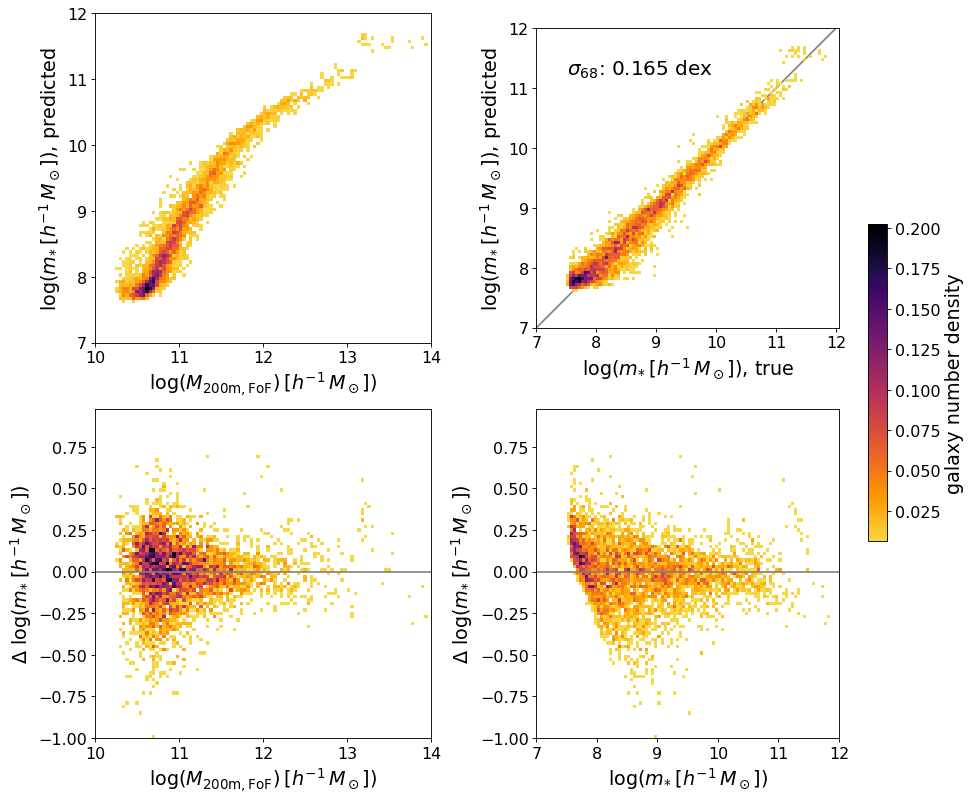
\includegraphics[width=0.7\columnwidth]{pred_mstellar.png}
    \caption{Predictions for the galaxy stellar mass $\mstellar$ using our invariant scalar features. The panels show the predicted stellar-to-halo mass relation, the predicted stellar mass compared to the true stellar mass, and the residuals of the stellar mass prediction compared to truth as a function of halo mass. The grey lines show zero error. The colorbar shows the number density of galaxies in units $(\hMpc)^{-3} \text{dex}^{-2}$, which takes into account the size of the box, the fraction of objects in the test sample, and the 2D histogram bin widths. We achieve accurate and precise predictions of the galaxy stellar mass with our invariant features.}
    \label{fig:mstellar}
\end{figure}

We focus on predicting the stellar mass of the central galaxy hosted by each DM halo, as this is the key quantity related to galaxy sample selection and is tightly correlated with other galaxy properties.
Our results with our fiducial feature set, the invariant scalar features with three radial bins, on our test sample of halos is shown in Figure~\ref{fig:mstellar}. 
In the top left we show the predicted stellar mass $\mstellar$ as a function of halo mass $\Mfof$; we see that we broadly recover the true shape of the stellar-to-halo mass relation. 
In the top right we show our predicted $\mstellar$ vs. the true $\mstellar$; our predictions are quite accurate, with a high density along the one-to-one line; the error $\sigma_{68}$, computed as the absolute symmetrized inner 68th percentile error, is 0.164 dex.

In the bottom row we show the absolute error (residuals) on our predictions as a function of halo mass and stellar mass.
We have larger errors at smaller halo and galaxy masses; this makes sense given the larger scatter in the stellar-to-halo mass relation at low halo masses, which is partially caused by shot noise dominating at those scales.
We also see an increase in error at high halo masses; this is related to the small sample size at those masses and the unbalanced training set in terms of halo size.
There is a clear artifact in the residuals as a function of stellar mass caused by our sample selection requirement that galaxies be composed of at least 50 star particles.
When the true stellar mass is very small, it is at the low edge of our training set and thus we are biased towards overpredicting it.
A practical tool could remedy this by using a wider training set than testing set to provide a buffer, or taking a multi-step approach to handle zero- and low-mass galaxies.  


\begin{figure}
    \centering
    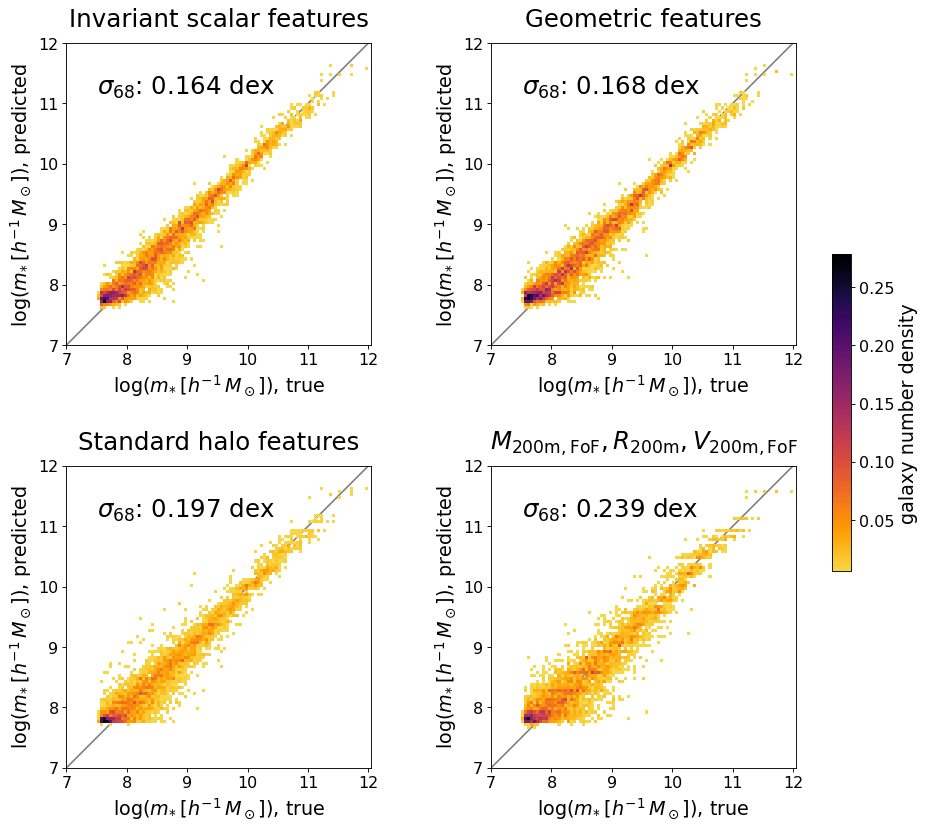
\includegraphics[width=0.7\columnwidth]{feature_comparison_mstellar.png}
    \caption{Predictions for the galaxy stellar mass based on different input feature sets: the invariant scalar features (our fiducial set); the components of the geometric features; a set of standard halo features; and only $\Mfof$, $\Rtwoh$, and $\Vfof$. These are detailed in \S\ref{sec:benchmarks}. The upper left panel is the same as the upper right panel in Figure~\ref{fig:mstellar}; the color bar is the same as in that figure as well. The invariant scalars approach outperforms the standard features in the stellar mass prediction, and significantly outperforms using only the mass and related scaling quantities. It very slightly outperforms the geometric feature set, which is not invariant to rotations.}
    \label{fig:mstellar_compare}
\end{figure}

We compare the performance our invariant scalars approach to other benchmark feature sets on galaxy stellar mass predictions in Figure~\ref{fig:mstellar_compare}.
Each panel shows the predicted vs. true stellar mass $\mstellar$ for a different feature set (detailed in \S\ref{sec:benchmarks}).
The invariant scalar features panel is reproduced from Figure~\ref{fig:mstellar}.
As expected, the worst-performing feature set is the one using only the basic global properties of the halo, $\Mfof$, $\Rtwoh$, and $\Vfof$ (recall that these are all directly related so this is essentially just a single scale), achieving just under a quarter of a dex in scatter.
We see some banding the predictions, likely due to the fact that this feature set can produce the mean stellar-to-halo mass relation but not the scatter.
The standard halo features, which includes the mass scale as well as a handful of shape and dynamical properties, performs better, with error reduced to under 0.2 dex. 

The geometric features produce still better predictions, suggesting that the detailed structure they encode---in both position and velocity space, and split into radial bins---adds significant information, giving an error 0.168 dex.
Somewhat surprisingly, we find that the invariant scalar features computed from these geometric features do not produce significantly improved predictions compared to the components of the geometric features.
The difference between these is that the geometric features are not invariant to rotations, while the scalar features are; both are invariant to translations, velocity boosts, and permutations, given how we construct the geometric features.
We expect that the invariance to rotations would become more important when using a smaller training set size, whereas the model seems able to learn the rotation invariance from our large and relatively homogenous training set.
It is also possible that the other symmetries are more dominant; in future work we could construct a benchmark that is not invariant to these symmetries for a clearer comparison.


\subsection{Predicting other baryonic properties}
\label{sec:pred_galprops}

\begin{figure}
    \centering
    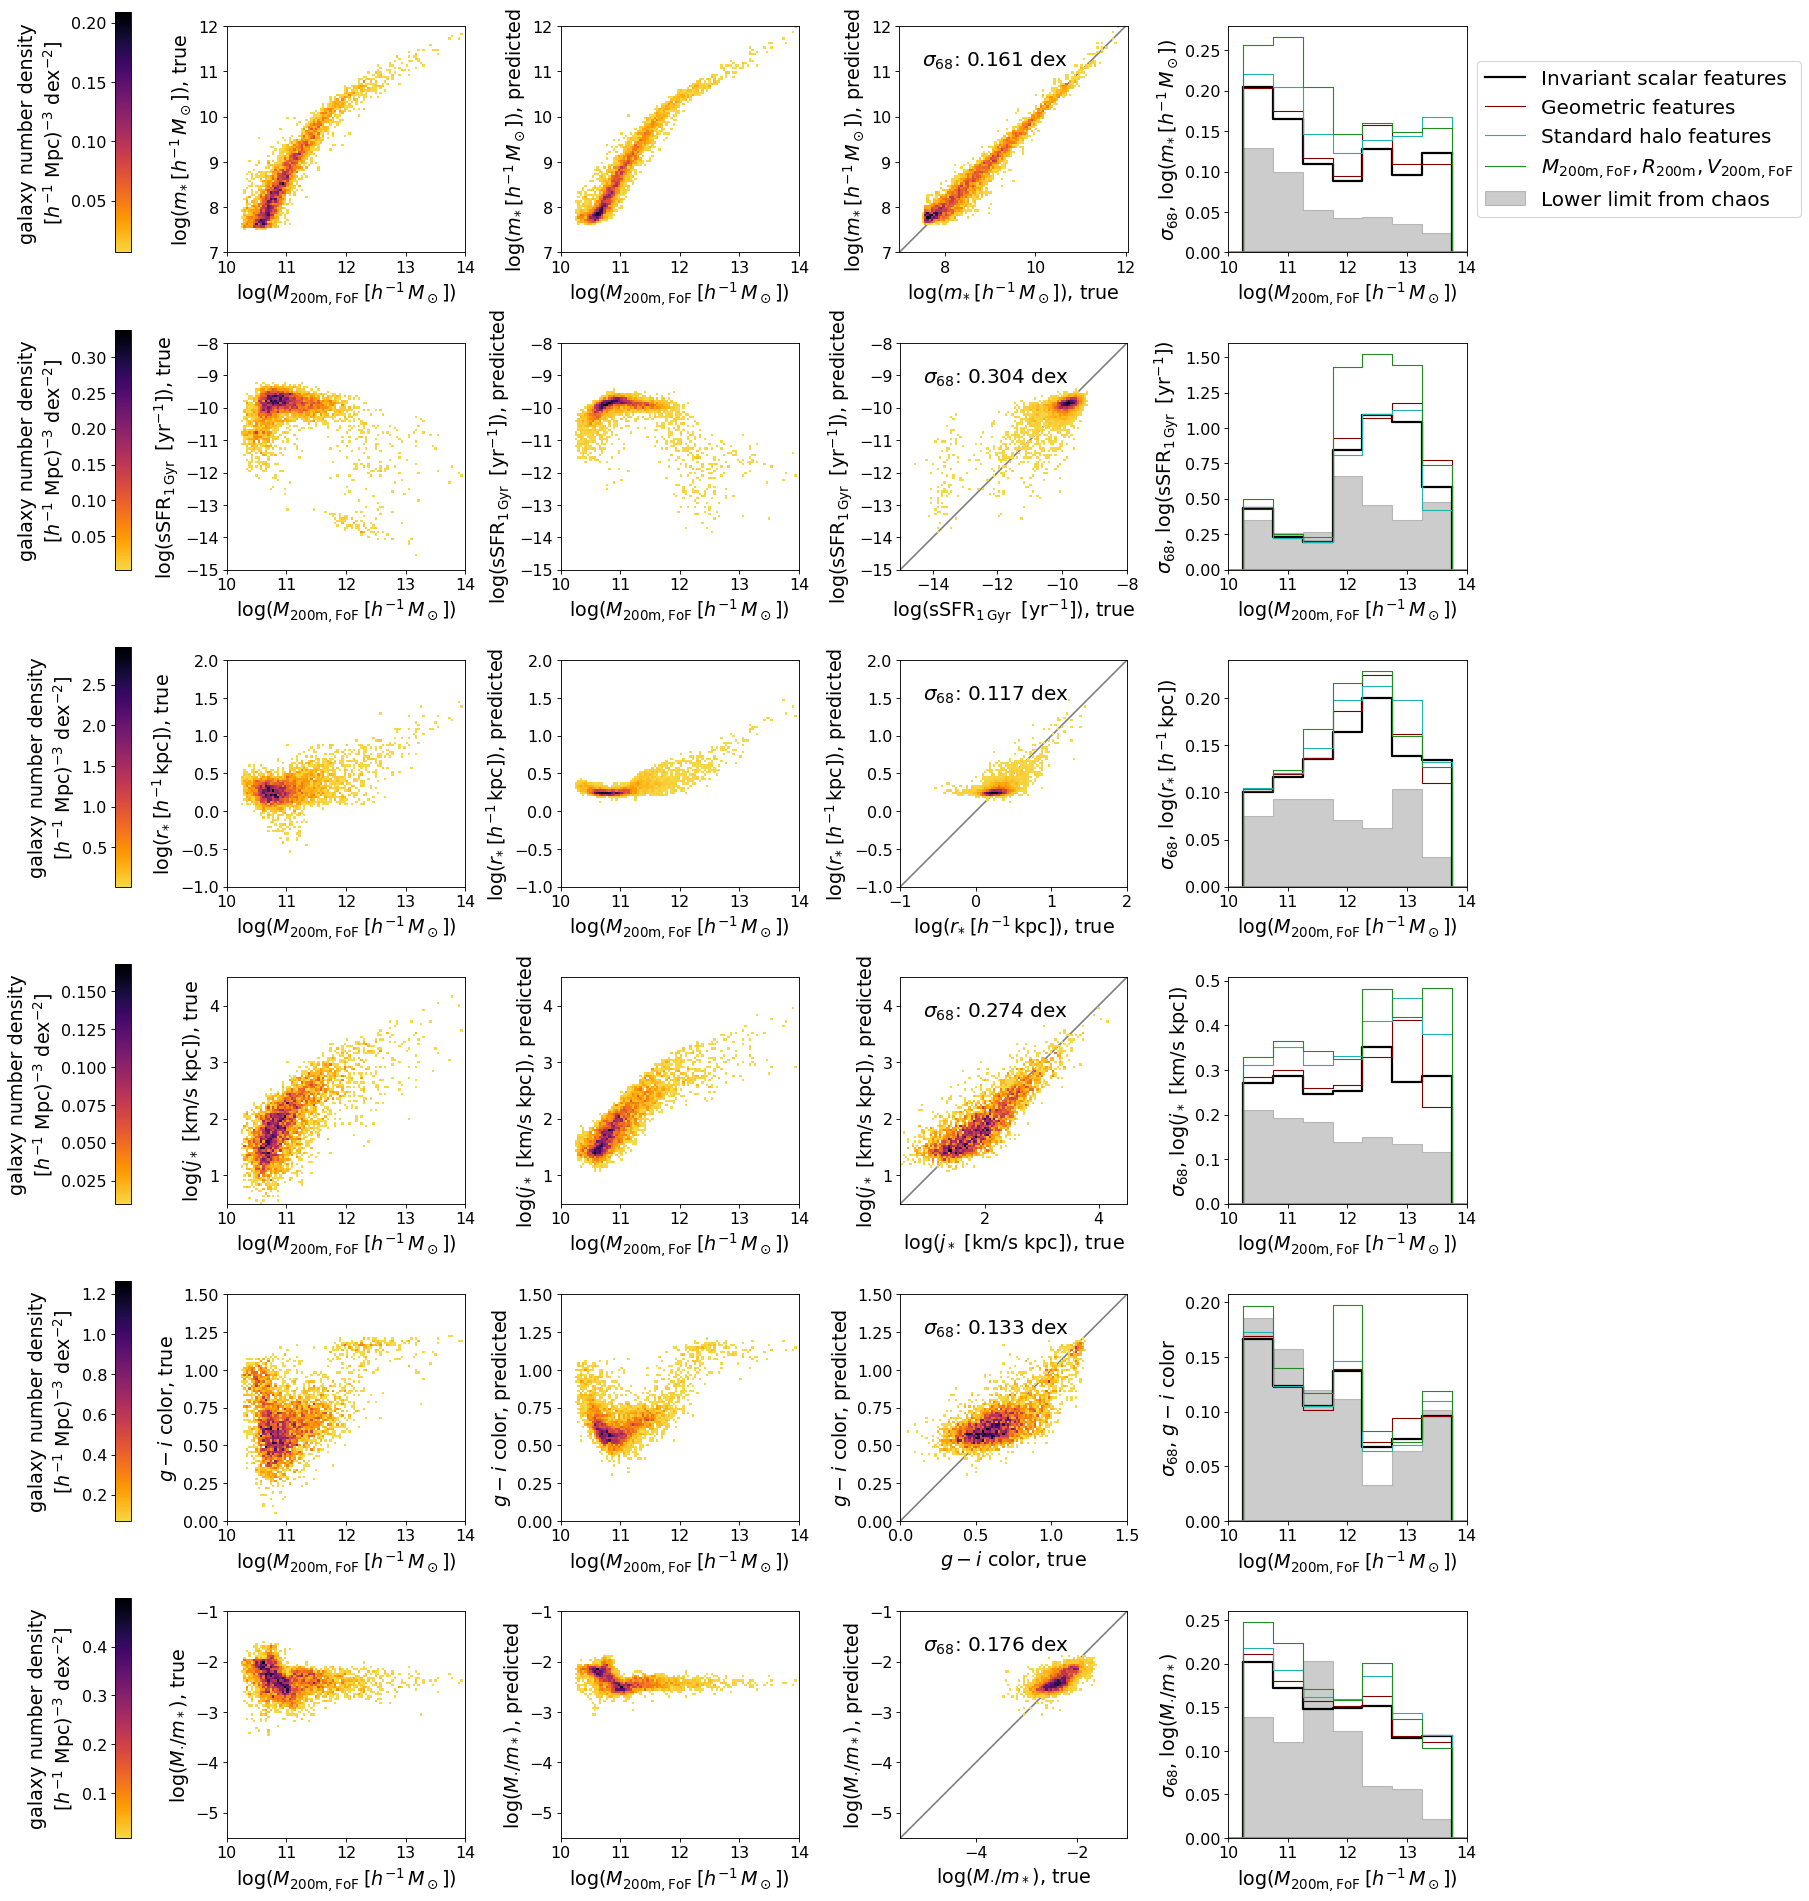
\includegraphics[width=0.87\columnwidth]{pred_galprops.png}
    \caption{Distributions and predictions of galaxy properties using our invariant scalars approach and other benchmark feature sets, for the test sample. 
    Each row shows a different galaxy property: stellar mass $\mstellar$, specific star formation rate $\ssfr$, stellar radius $\rstellar$, specific stellar angular momentum $\jstellar$, $\gminusi$ color, and black hole mass per stellar mass $\mbhpermstellar$. 
    The left column shows the property as a function of halo mass $\Mfof$. 
    The second column is the predicted distribution as a function of halo mass, and the third compared to the true property, using the fiducial invariant scalar features.
    The right is the binned error as a function of halo mass, comparing the scalar features (thick black), geometric feature components (red), standard features (blue), and mass scale features (green); the grey shaded region shows the lower limit from chaos.
    For most of the galaxy properties, the scalars slightly outperform the other features, but many properties are limited by chaos.
    }
    \label{fig:galprops}
\end{figure}

We show the results of our predictions on other galaxy and baryonic properties in Figure~\ref{fig:galprops}.
In the left two columns, we show the true and predicted distributions of properties as a function of halo mass $\Mfof$, where the predictions are with our fiducial invariant scalar features.
We see that we broadly reproduce the shape of the distribution for all of the properties. 
However, there are significant differences; noteably, nearly all of our predictions fail to reproduce the full scatter of the true distributions, tending towards the mean.
Generally, the regions of poor prediction indicate that either our features are not informative enough, our model is not performant enough, or there is a fundamental limitation in the amount of information accessible---or some combination of these three.

We investigate the final possibility by comparing the error in our results to the scatter from chaos, as computed from the ``butterfly'' simulations of \cite{Genel2019} (described in \S\ref{sec:galprops}), which represents a limit to the retrievable information.
This is shown as a function of halo mass in the grey shaded region in the final column, compared to the binned error of our predictions.
We see that for some properties in some regimes, we are indeed at or near the chaotic limit, where we expect the rest of the information is destroyed by the chaotic effects of evolution.
This is the case for the $\ssfr$ and $\rstellar$ at low halo masses, for $\gminusi$ color at all masses, and $\mbhpermstellar$ at intermediate masses.
For these cases, we are able to reproduce the relatively complex shape of the property distribution as a function of halo mass: for instance for the $\ssfr$ we accurately predict the sharp transition from large scatter at very low halo mass to low scatter at intermediate halo mass, and for $\gminusi$ color we predict the non-monotonic shape of the distribution vs. halo mass, including the large colors of the high-mass galaxy population.
In some bins we are achieving results below the chaotic limit; this may be because this is a somewhat optimistic limit as it is computed from a slightly higher resolution simulation, and also possibly due to small number statistics (generally for the butterfly simulations, and especially for the high mass bins in both).

There are some populations that our predictions fail to reproduce, somewhat separate from the low-scatter issue.
For instance, we do not predict the very low $\rstellar$ ``fin'' at low halo masses, leading to consistent over-predictions in that bin.
Our model also struggles to handle very low values, such as in the $\ssfr$ distribution where we replaced the value of galaxies with no star formation with a small limit, as can be seen in the intermediate-to-high mass regime (where galaxies are more likely to be quenched).
We see that our predictions do not separate out this population, instead predicting a continuous distribution of specific star formation rates at those masses.
While some of our predictions of baryonic properties are impressive and show that there is significant information in halo shape relevant to galaxy properties, our results broadly align with other recent findings that baryonic properties beyond stellar mass are difficult to predict using halo features \citep{de_santi_mimicking_2021,stiskalek_scatter_2022}.

In the right column of Figure~\ref{fig:galprops}, we show the comparison between our invariant scalars approach with the other benchmark feature sets.
We find that while the scalars generally outperform the other features, the differences are not particular pronounced for most properties and scales.
The clearest improvements of the scalars over the standard features are seen in predicting the stellar mass $\mstellar$, as discussed in \S\ref{sec:pred_mstellar}, and the specific stellar angular momentum $\jstellar$; the latter may be thanks to our inclusion of high-order velocity-space features, while the standard features only use the velocity dispersion and spin.
Similarly to the stellar mass case, we do not see a clear difference between predictions with the scalar features and geometric features, indicating that the model is able to learn the rotational invariance from the data even when the features are not invariant.


\subsection{Predicting the halo mass assembly history}


\begin{figure}
    \centering
    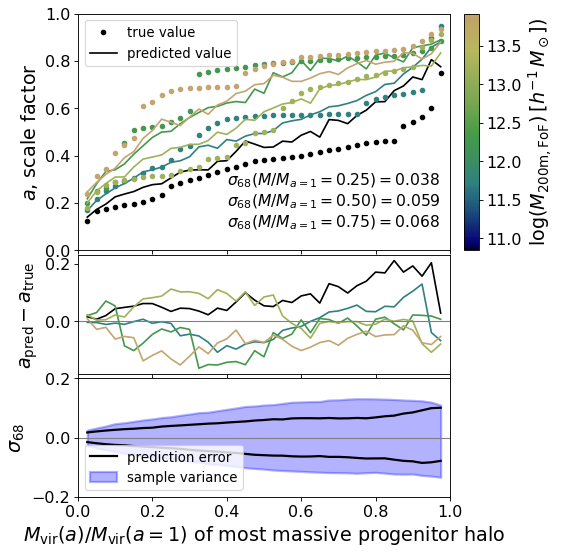
\includegraphics[width=0.6\columnwidth]{pred_amfrac.png}
    \caption{The predicted mass assembly history (MAH) of a halo based on the invariant shape scalars, parameterized by the scale factor at which the halo's most massive progenitor accreted a given fraction of its mass. The top panel shows the MAHs of a random selection of halos from the test set (closed circles), and the predicted scale factor at each mass fraction. The middle panel shows the fractional residuals between the two, and the bottom shows the inner 68th percentile of the predictions for all of our test set, compared to that of the distribution of MAHs used in training. \ksf{rn im plotting test set for latter, make sure to switch to test!}}
    \label{fig:mah}
\end{figure}


\begin{figure*}
    \centering
    \subfloat[\label{fig:pred_amfrac_hi}]{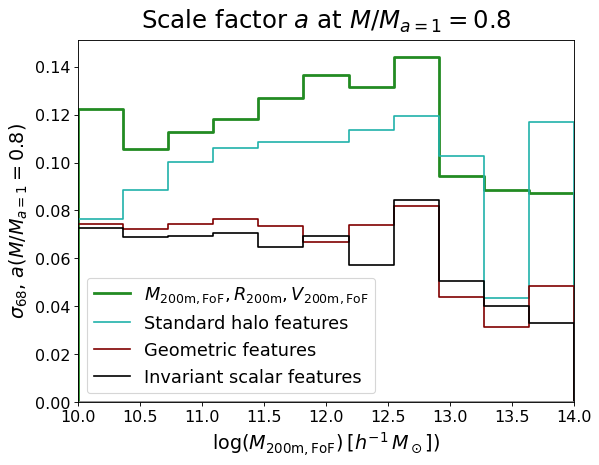
\includegraphics[width=0.45\textwidth]{pred_amfrac_hi.png}}
    \hspace{2em}
    \subfloat[\label{fig:pred_amfrac_lo}]{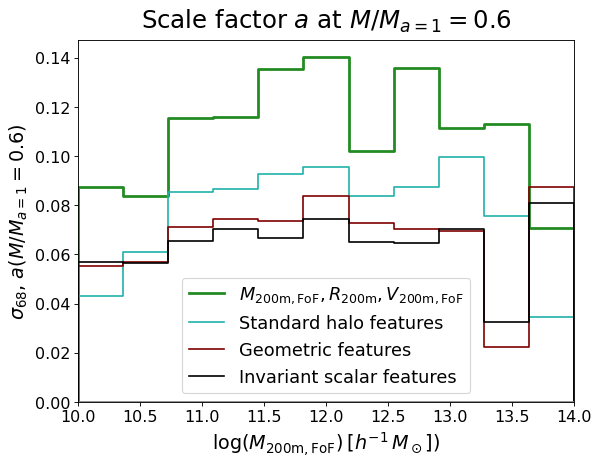
\includegraphics[width=0.45\textwidth]{pred_amfrac_lo.png}}
    \caption{}
\end{figure*}


% \subsection{Understanding the relative importance of the halo shape features}

% The feature subsets we consider are: only mass features; mass and position features; mass and velocity features; mass, position and velocity features.
% We also investigate limiting to certain orders in $O(x)+O(v)$: 0, 2, and 4.
% Finally, we consider different numbers of bins, as well as excluding cross-bins.

% \begin{figure}
%     \centering
%     %\includegraphics{}
%     \caption{The precision on the predictions of the given property when using the denoted subset of invariant scalars.}
%     \label{fig:features}
% \end{figure}


\section{Discussion}
\label{sec:discussion}

Topics/points for discussion section:
\begin{itemize}
    \item Understanding of important features (what do they mean, relationship to currently used features)
    \item Application of approach to useful tasks (constructing mock catalogs, predicting galaxy properties in larger \& higher res simulations and being able to construct many realizations)
    \item The inference problem: going from galaxies to DM
    \item Feature construction choices (e.g. could construct geometric features other ways like with spherical harmonics)
    \item Future goal to move away from halo framework and work on full particle distribution, starting from e.g. density peaks. Intermediate task is to start from halo centers but include all particles, not just those in FoF group
    \item Future work to look at impact of larger-scale environment, incorporate it in input features
    \item Other properties we should predict (position: discuss offsets bw dark and hydro; spin: pseudo-vector)
    \item particles have large time derivative; galaxy has relatively small time derivative! we could show this with our scalars. discuss time dependence.
\end{itemize}

\section{Summary}
\label{sec:summary}


\section{Chapter Acknowledgements}
The authors would like to acknowledge very helpful discussions with Soichiro Hattori, Austen Gabrielpillai, Ben Blum-Smith, Weichi Yao, Scott Tremaine, Rachel Somerville, Derek Lim, and Benjamin Wandelt.
The authors also thank useful feedback by participants of the Flatiron CCA Astrodata Group, Galaxy Formation Group, and Cosmology X Data Science Group.
This research was performed in part at the Coworking Retreat on Equivariant Machine Learning held at the Johns Hopkins University in March 2023.
K.S.F.~is supported by the NASA FINESST program under award number 80NSSC20K1545.
This research made use of computational resources at New York University; we thank the NYU high-performance computing team.

\chapter{QUaia, the \emph{Gaia}–unWISE Quasar Catalog: An All-Sky Spectroscopic Quasar Sample}
\setcounter{section}{-1}
\label{chp-quaia}
%\graphicspath{{figures/figures_quaia/}}

% % latex things
% \newcommand\minput[1]{%
%   \input{#1}%
%   \ifhmode\ifnum\lastnodetype=11 \unskip\fi\fi}

%\sloppy\sloppypar\frenchspacing

% Loads external quantities
% via https://tex.stackexchange.com/questions/321346/how-to-read-a-variable-from-a-file-in-latex
% and https://tex.stackexchange.com/questions/609934/datatools-dtlfetch-returns-last-found-value-instead-undefined-value-if-entry
\DTLloaddb[noheader, keys={thekey,thevalue}]{quantities}{data/data_quaia/quantities.txt}
\DTLnewdbonloadfalse % allows appending data
\DTLloaddb[noheader, keys={thekey,thevalue}]{quantities}{data/data_quaia/quantities_comparison.txt}

\newcommand{\val}[1]{% 
    % \DTLgetvalueforkey{<cmd>}{<key>}{<db name>}{<ref key>}{<value>}
    % This (globally) sets cmd (a control sequence) to the value of the key specified by <key> (note that this <key> is our value!)
    % in the first row of the database called <db name> which contains the key <ref key> which has the value <value>.
    \DTLgetvalueforkey{\scratchmacro}{thevalue}{quantities}{thekey}{#1}%
    % This checks if hcmdi is null where hcmdi is a control sequence, if it is, then htrue parti is done, otherwise hfalse parti is done.
    % end with xspace
    \DTLifnull{\scratchmacro}{UUU}{\scratchmacro}\xspace
}


\section{Chapter Abstract}
\Gaia DR3 contains \val{N_gall} sources that are classified as possible quasars, with estimated redshifts from low-resolution BP/RP spectra.
These quasar candidates comprise an unprecedented resource for extragalactic and large-scale structure science: they are all-sky and have a median redshift of $z \sim \val{z_med_gall}$, hence covering more comoving volume than any other quasar sample.
While the quasar candidate catalog is highly complete, it has low purity.
Further, $\val{p_outliers_gall_zgaia_dzhi_Glo}\%$ of quasar candidates with $G<\Glo$ have highly inaccurate redshift estimates ($|\dz| > \val{dzhi}$) when compared to redshifts obtained by the Sloan Digital Sky Survey (\SDSS).
In this work, we construct a quasar catalog based on the \Gaia candidates sample as well as unWISE infrared observations (based on the Wide-Field Infrared Survey Explorer survey) that is suitable for cosmological and other analyses.
To decontaminate the sample, we apply cuts based on proper motions and \Gaia and unWISE colors, reducing the number of contaminants by an estimated \val{factor_reduction_contaminants}.
We improve the redshifts by training a $k$-nearest neighbors model based on colors and \Gaia redshift estimates with \SDSS redshift labels, and achieve a sample with only $\val{p_outliers_zspz_dzhi_Glo}\%$ ($\val{p_outliers_zspz_dzmid_Glo}\%$) catastrophic redshift errors with $|\dz| > \val{dzhi}$ ($\val{dzmid}$) on our spectro-photometric redshift estimates, a reduction of \val{factor_reduction_outliers_dzhi_Glo} (\val{factor_reduction_outliers_dzmid_Glo}) compared to the \Gaia redshifts.
The final catalog, the \catalog (\cat), has \val{N_gcathi} quasar candidates with a $G<\Ghi$, and \val{N_gcatlo} candidates in the even cleaner $G<\Glo$ sample.
We construct a rigorous all-sky selection function model for the sample, incorporating dust extinction, stellar source crowding, and the \Gaia scanning law. 
We verify our catalog against other quasar catalogs, and describe possible applications and limitations.
The catalog is publicly available \texttt{here}. 


\section{Introduction}

Quasars are powerful tools for many fields of astrophysics. 
They are key probes of accretion physics (e.g. \citealt{SunyaevZeldovich1970, yu_quasar_2020}), which informs the evolution of active galactic nuclei (AGN). 
The evolution of quasars and their host galaxies are intertwined, giving insight into supermassive black hole growth (e.g. \citealt{hopkins_unified_2006}) as well as massive galaxy formation (e.g. \citealt{kormendy_coevolution_2013}).
Studies of the quasar distribution can also be used to understand black hole evolution (e.g. \citealt{powell_clustering_2020}) and halo masses and environmental effects (e.g. \citealt{dipompeo_characteristic_2017}).
Quasars are  key background sources for other cosmic phenomena such as gravitational lenses (e.g. \citealt{claeskens_gravitational_2002}), and quasar spectra encode the properties of the intergalactic medium via the Lyman alpha forest (e.g. \citealt{rauch_lyman_1998}). 

Quasars are key tracers for large-scale structure cosmology.
They reside in peaks of the dark matter distribution and their clustering can be used to measure cosmological parameters, including the baryon density $\Omega_b$, the cosmological constant $\Omega_\Lambda$, the Hubble distance $D_H$, and the growth rate of structure $f\sigma_8$ (e.g. \citealt{yahata_large-scale_2005, hou_completed_2020}).
Cross-correlations between quasars and other tracers provide measurements of key quantities, such as with photometric galaxy samples to measure the baryon acoustic feature (e.g. \citealt{}), with cosmic microwave background lensing to constrain quasar bias (e.g. \citealt{sherwin_atacama_2012}), and with foreground galaxies as a probe of weak lensing (e.g. \citealt{menard_cosmological_2002, scranton_detection_2005, zarrouk_baryon_2021}).
They can also be used as standardizable candles to measure the expansion rate of the universe (e.g. \citealt{setti_hubble_1973, risaliti_hubble_2015, lusso_quasars_2020}).
Finally, the quasar distribution provides a test of the cosmological principle of isotropy and homogeneity (e.g. \citealt{secrest_test_2021, dam_testing_2022}).

Many surveys have observed and cataloged quasars, with several million currently identified across surveys.
The latest Sloan Digital Sky Survey data release, DR16, includes a highly complete catalog of 750,414 quasars with spectroscopic redshifts \citep{lyke_sloan_2020}.
Photometric surveys observe a much larger large number of quasars, at the expense of low redshift accuracy; nearly three million quasars with reliable photometric redshifts have been cataloged \citep{kunsagi-mate_photometric_2022}, including with WISE \citep{wright_wide-field_2010} which imaged the entire sky and PAN-STARRS \citep{chambers_pan-starrs1_2019} which observed three-quarters of the sky.
Upcoming surveys will observe even more quasars: the Dark Energy Spectroscopic Instrument (DESI, \citealt{Aghamousa2016}) expects to obtain spectra for 3 million quasars, and the Rubin Observatory's LSST will photometrically observe upwards of 10 million quasars \citep{ivezic_lsst_2016}.
However, none of these quasar catalogs is both all-sky and contains precise redshift information.
The recently released \Gaia DR3 quasar candidates \citep{gaia_collab_gaia_2022} constitute a new sample that fills this gap. 

The \Gaia quasar catalog presents a new opportunity to explore these science questions.
While the \Gaia satellite was designed to map the stars in the Milky Way \citep{gaia_collaboration_gaia_2016}, it broadly observes bright objects in the sky, which includes many extragalactic sources. 
In DR3, the \Gaia collaboration released a sample of 6,649,162 quasar candidates that were incidentally observed during the survey \citep{gaia_collab_gaia_2022}.
The sources cover the entire sky and have \Gaia BP/RP spectra, low-resolution spectra covering the wavelength range 330-1050 nm. 
These spectra allow for redshift estimates of the sources, with $\val{p_acc_gall_zreliable_zgaia_dzlo}\%$ having a precision of $|\dz| < \val{dzlo}$ compared to \SDSS redshifts when no redshift warning flags are set, which is the case for $\val{p_zreliable_gall}\%$ of the sample (for the full sample, this decreases to $\val{p_acc_gall_zgaia_dzlo}\%$).
While not as precise as high-resolution spectroscopic redshifts, they are significantly better than photometric redshifts. 
The median redshift of the sample is $z=\val{z_med_gall}$. 
The \Gaia quasar candidate sample was constructed for completeness over purity, and has an estimated purity of 52\%; the \Gaia collaboration also suggests criteria for a higher purity ($\sim$95\%) sub-catalog of $\sim$1.9 million quasars.
Overall, the sample presents an unprecedented resource for quasar science and cosmology.

There are two main issues with this raw \Gaia sample.
First, the sample contains a large number of non-quasar contaminants.
Second, a significant fraction of the redshift estimates are catastrophic errors, due to emission line misidentification given the limitations of the spectra.
In this work, we construct a clean quasar catalog with low contamination and improved redshift estimates, with the particular goal of building a catalog appropriate for large-scale structure analyses, as well as other quasar science.
For both of these, we rely on cross-matches with unWISE observations of the quasars, which adds key infrared information.
To filter out contaminants, we apply color cuts based on the \Gaia and WISE photometry, as well as a proper motion cut.
To improve the redshifts, we identify quasars that are also observed by \SDSS for which we have highly precise spectroscopic redshifts, and train a $k$-Nearest-Neighbors ($k$NN) model based on their photometry and \Gaia redshift estimates.
Further, the \Gaia quasar candidates sample has strong systematic imprints from various observational effects, such as galactic dust.
We fit a model for the selection function based on observational templates using a Gaussian process; this map is a key ingredient in many analyses.

This paper is organized as follows.
In \S\ref{sec:data}, we describe the initial data sets used in the construction of the catalog.
The catalog construction is detailed in \S\ref{sec:construction}.
In \S\ref{sec:catalog}, we present the final catalog and perform verification and comparisons to other samples, and outline the data format.
We summarize the catalog and describe data access in \S\ref{sec:summary}.

\section{Initial Data Sets}
\label{sec:data}

\begin{figure}
    \centering
    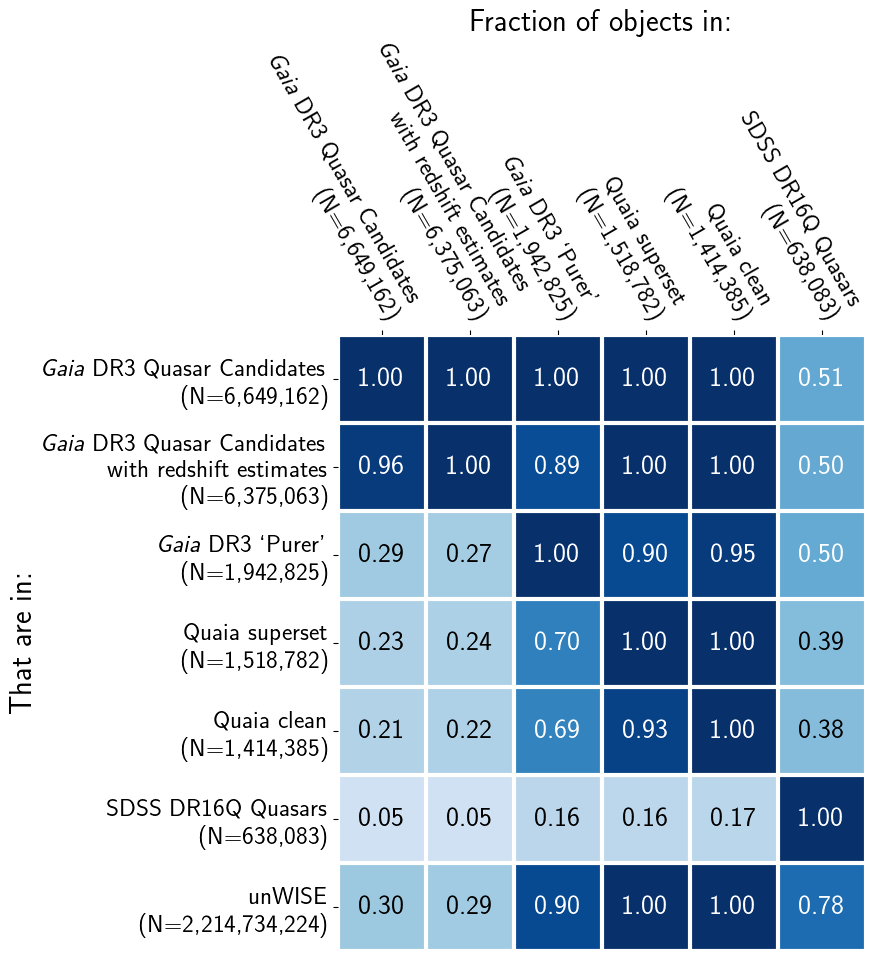
\includegraphics[width=0.6\textwidth]{frac_matrix.png}
    \caption{A summary of the overlaps between the various data sets and subsamples used in this work. The values describe the fraction of objects in each column's sample that are in each row's sample. Note that we only list \unWISE as a row because the inverse is not relevant to this work.}
    \label{fig:frac_matrix}
\end{figure}

\subsection{The \Gaia DR3 quasar candidate sample}
\label{sec:data_gaia}

\begin{figure}
    \centering
    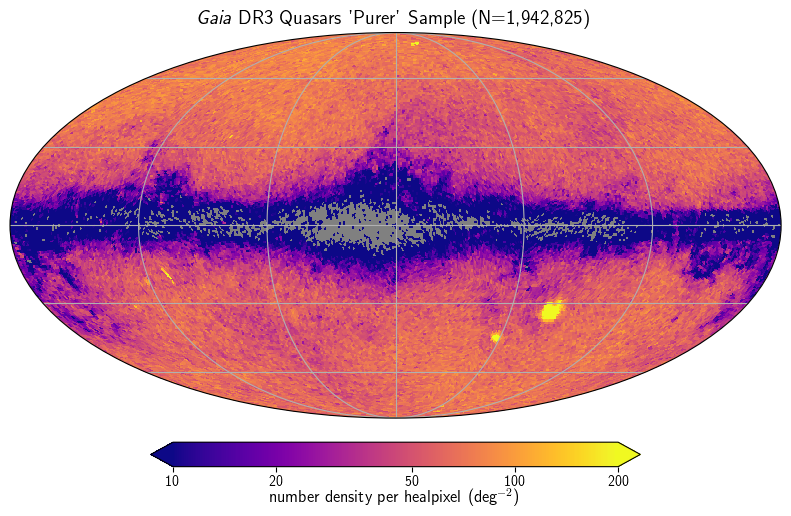
\includegraphics[width=0.6\textwidth]{gpurer_2d.png}
    \caption{Sky distribution of the quasar candidates in the \Gaia DR3 ``purer'' quasar sample, in Galactic coordinates and displayed using a Mollweide projection.}
    \label{fig:gaia_2d_purer}
\end{figure}

While performing its all-sky survey of the Milky Way, the \Gaia satellite \citep{gaia_collaboration_gaia_2016} also observed millions of extragalactic objects.
These sources---both quasar and galaxy candidates---were first released in \Gaia DR3 \citep{gaia_collaboration_gaia_2022, gaia_collab_gaia_2022}.
\Gaia obtained BP/RP spectra of the sources, which are low-resolution spectra with relatively narrow wavelength ranges; the blue photometer (BP) covers 330-680 nm and has $30 \leq R \leq 100$ and the red photometer (RP) covers 640-1050 nm \citep{carrasco_internal_2021} with $70 \leq R \leq 100$.
The raw spectra are not released by \Gaia (besides a small subsample---the rest will be released in \Gaia DR4), but redshift estimates and other derived information are contained in the catalogs.

The quasar candidates were selected based on multiple classifiers and criteria, described in detail in \cite{gaia_collab_gaia_2022}.
The majority (5.5 million) of the quasar candidates were identified with the Discrete Source Classifier (DSC) module (detailed in \cite{delchambre_gaia_2022}, a machine learning model that takes as input the source's BP/RP spectrum, $G$-band magnitude, $G$-band variability, parallax, and proper motion, and outputs a class label based on \SDSS spectroscopic classifications.
Given these \SDSS labels, the results of this module will inherit many of the same selection effects as \SDSS, such as missing highly reddened quasars.
DSC is estimated to have a completeness of over $90\%$ and a purity of around $24\%$ for quasars.
Another machine learning model selected over 1 million sources were contributed based on their variability, as active nuclei have time-variable accretion; the model inputs were statistics of time series data in all \Gaia bands as well as photometric and astrometric quantities, as detailed in \cite{rimoldini_gaia_2023}. 
Additionally, a set of nearly 1 million sources were selected based on their surface brightness profile; this selection used existing major quasar catalogs to compile an initial list of sources, which were then processed by the \Gaia surface brightness profile module \cite{ducourant_gaia_2022}.
This module included quasars in the candidates catalog which passed certain criteria, including having \Gaia observations covering $>86\%$ of the source's surface area and a confident assessment (positive or negative) of host galaxy presence.
Finally, the 1.6 million sources used to define the \Gaia-CRF3 celestial reference frame were contributed, which are based on cross-matches of \Gaia to external quasar catalogs.
A large fraction of sources are identified as quasars by multiple of these methods; the overlapping contributions are shown in Figure 3 of \cite{gaia_collab_gaia_2022}.
The full quasar candidate sample contains \val{N_gall} sources\footnote{The \Gaia DR3 quasar candidates sample, and all other \Gaia data, can be downloaded at \url{https://gea.esac.esa.int/archive}.}, selected for high completeness, but with a low purity estimated to be around 52\% \citep{gaia_collab_gaia_2022}.
We show the overlaps between this \Gaia quasar candidate sample and other samples and subsamples used and constructed in this work in Figure~\ref{fig:frac_matrix}.

Most of the quasar candidates (\val{N_gall_wqsoc}) are assigned redshifts using the Quasar Classifier (QSOC) module, which uses a chi-squared approach on the quasars' BP/RP spectra compared to composite spectra from \SDSS DR12Q \citep{delchambre_gaia_2022}.
We refer to these \Gaia redshift estimates as $\zgaia$.
Many of these redshifts are determined by a single line due to the narrow spectral range, resulting in aliasing issues when lines are misidentified (see Figure 15 in \cite{delchambre_gaia_2022}).
% these numbers are cited in delchambre paper, so not filled in automatically
An estimated 63.7\% of the redshifts have $|\Dz| < 0.1$, increasing to 97.6\% for quasar candidates with no redshift warning flags (this is the case for nearly $80\%$ of quasars with $G<18.5$, but decreases to less than 20\% for $G>19.5$).

\cite{gaia_collab_gaia_2022} provides a query to select a purer subsample of the quasar candidates.
It requires higher quasar probability thresholds from the various classifiers and excludes surface-brightness-selected galaxies that have close neighbors.
This results in \val{N_gpurer} sources with an estimated purity of 95\%; 1.7 million of these have Gaia redshifts. 
The sky distribution of this sample is shown in Figure~\ref{fig:gaia_2d_purer}.
The sample has a low density in the galactic plane, because the selection was trained on the \SDSS quasar sample which does not contain reddened sources (as it is based on a color selection), and overdensities around the Magellanic Clouds, as the sample still contains stellar contaminants.

For our analysis, we start with the full quasar candidate sample, rather than the ''purer'' sample or cutting on other \Gaia pipeline flags, to allow for higher completeness and minimize reproducing biases; we compare our catalog to the \cite{gaia_collab_gaia_2022} purer subsample in \S\ref{sec:comparison}.
We construct a \emph{superset} that contains all of the information needed for catalog construction: we require that sources are in the \Gaia quasar candidates table, have \Gaia $G$, $BP$, and $RP$ measurements, have \unWISE $W1$ and $W2$ observations (described in \S\ref{sec:data_wise}), have \Gaia-estimated QSOC redshifts, and make a maximum $G$-magnitude cut of $G < \Gmax$.
This magnitude cut was chosen to be slightly deeper than our desired catalog magnitude limit of $G<\Ghi$, in order to provide a buffer for redshift estimation.
This results in a superset with \val{N_gsup} sources, $\val{p_gsup_gall}\%$ of the \Gaia quasar candidates table.
We call our final catalog the \catalog (\cat), so we refer to this as the \cat superset.


\subsection{The \unWISE Quasar Sample}
\label{sec:data_wise}

We use the \unWISE survey to contribute infrared (IR) photometry to \Gaia sources \citep{lang_unwise_2014,meisner_unwise_2019}.
The \unWISE coadds combine data from NEOWISE \citep{mainzer_preliminary_2011} with the original WISE \citep{wright_wide-field_2010} survey, providing a time baseline fifteen times longer.
Compared to the original \textsl{AllWISE} catalog, \unWISE has deeper imaging and improved modeling of crowded fields.
The \unWISE catalog \citep{schlafly_unwise_2019} contains measurements in the $W1$ (3.4 $\mu$m) and  $W2$ (4.6 $\mu$m) bands for over 2 billion sources.
We do not use the $W3$ and $W4$ bands as these do not go as deep as we need.
We perform a cross-match of the \Gaia quasar candidate sample to \unWISE sources within 1''\footnote{We use NOIRLab's cross-match service to perform this operation, available at \url{https://datalab.noirlab.edu/xmatch.php}.}, and obtain \val{N_gall_xunwise} matched sources.
We also cross-match the \SDSS training and validation samples (\S\ref{sec:data_sdss_quasars}, \S\ref{sec:data_contaminants}) to \unWISE.

When combined with optical photometry, \unWISE IR color information is very useful for identifying quasars and distinguishing them from contaminants.
This photometry also contains useful redshift information; recent approaches to estimate redshifts from photometry with neural networks achieve a mean $|\Dz|\sim 0.22$ \citep{yang_quasar_2017, jin_efficient_2019, kunsagi-mate_photometric_2022}.
In our case of redshift estimates from narrow-range BP/RP spectra, we expect IR photometry to add information that can break line identification degeneracies in order to improve estimates.
We incorporate the $W1$ and $W2$ bands into both our quasar selection (\S\ref{sec:decontam}) and redshift estimation (\S\ref{sec:redshifts}) procedures.


\subsection{The \SDSS DR16 quasar sample}
\label{sec:data_sdss_quasars}

The Sloan Digital Sky Survey released the largest spectroscopic quasar catalog in DR16\footnote{The \SDSS DR16Q quasar catalog is publicly available at \url{https://www.sdss.org/dr16/algorithms/qso_catalog}.} \citep{lyke_sloan_2020}.
It combines new sources from the extended Baryon Oscillation Spectroscopic Survey (eBOSS), part of \textsl{SDSS-IV}, with previously observed sources from the earlier \SDSS campaigns.
The catalog contains 750,414 quasars, with an estimated 99.8\% completeness and $98.7-99.7$\% purity.
We remove sources with redshift warnings, \texttt{ZWARNING}!=0, as well as a handful of sources with unreasonably low or negative redshift estimates ($z<0.01$). 
This results in \val{N_sqall} sources, which is the sample shown in Figure~\ref{fig:frac_matrix}.
We cross-match these with the \Gaia catalog, as well as \unWISE (\S\ref{sec:data_wise}), using a maximum separation of 1'' on the sky.
We remove sources with fewer than 5 observations in $BP$ (\texttt{phot\_bp\_n\_obs}) or $RP$ (\texttt{phot\_rp\_n\_obs}), following \citep{bailer-jones_dsc_2021}, as well as sources that are duplicated in the \SDSS star or galaxy samples (\S\ref{sec:data_contaminants}) 
This results in \val{N_squasars_unwise} sources with both \Gaia and \unWISE observations that pass these criteria.

We use these to calibrate the cuts to make to decontaminate our sample (\S\ref{sec:decontam}); for this purpose we only keep sources that are also in the \cat superset (sources that are in the \Gaia quasar candidates table, have all necessary \Gaia and \unWISE photometry, \Gaia-estimated QSOC redshifts, and $G < \Gmax$).
This sample contains \val{N_squasars_sup} quasars.
We also use this sample (after applying the cuts described in \S\ref{sec:decontam}) to train our redshift estimation model (\S\ref{sec:redshifts}).
While this spectroscopic sample has quite high completeness and accurate redshift information, we note that it is still imperfect, contains selection effects, and represents only a particular definition of a quasar; these issues will propagate to our catalog.


\subsection{Contaminant samples: galaxies and stars}
\label{sec:data_contaminants}

To guide the decontamination of our catalog (\S\ref{sec:decontam}), we compile known contaminant samples, namely galaxies and stars.
For the galaxy sample, we use \SDSS spectroscopic galaxies from DR18\footnote{\SDSS DR18 data can be accessed at \url{https://skyserver.sdss.org/CasJobs/jobdetails}.}.
Following \citep{bailer-jones_dsc_2021}, we include all galaxies with class label \texttt{GALAXY} in the \texttt{SpecObj} table, exclude galaxies with subclass labels \texttt{AGN} or \texttt{AGN BROADLINE}, and exclude sources with redshift warnings, \texttt{zWarning=0}.
We cross-match these with \Gaia DR3 and \unWISE with a 1'' radius, and remove sources with fewer than 5 observations in $BP$ or $RP$, as for the \SDSS quasars.
We also remove apparent stellar contaminants from the galaxies sample with the cut in $G-RP$ and $BP-G$ from equation (1) of \cite{bailer-jones_quasar_2019}, and additionally remove sources duplicated in the \SDSS quasar or star samples.
This leaves \val{N_sgals_unwise} cross-matched \SDSS galaxies in our sample; \val{N_sgals_sup} of these are in the \cat superset.

For the star sample, we also use \SDSS DR18 sources, selecting objects with class label \texttt{STAR} in the \texttt{SpecObj} table.
As for the quasars and galaxies, we cross-match these with \Gaia DR3 with a 1'' radius and remove sources with fewer than 5 observations in BP or RP, and remove sources duplicated in the other samples.
This results in a stellar sample with \val{N_sstars_unwise} cross-matched \SDSS-\Gaia stars, with \val{N_sstars} of these in the superset.

For the decontamination procedure, we also compile a sample of sources in or near the LMC or SMC, as most of these will be stellar contaminants but have different properties than the \SDSS star sample.
To do this, we select all sources in the \Gaia quasar candidates table that are within 3 degrees of the center of the LMC or 1.5 degrees from the center of the SMC.
While this may include non-MC stars, we have chosen these fairly narrow radii in order to capture mostly MC stars and few potential quasars.
Additionally requiring that these have \unWISE photometry, this gives \val{N_mcs_unwise} MC-adjacent stars; \val{N_mcs_sup} are in the superset.


\section{Catalog construction}
\label{sec:construction}

\subsection{Decontamination with proper motions and \unWISE colors}
\label{sec:decontam}

\begin{figure}
    \centering
    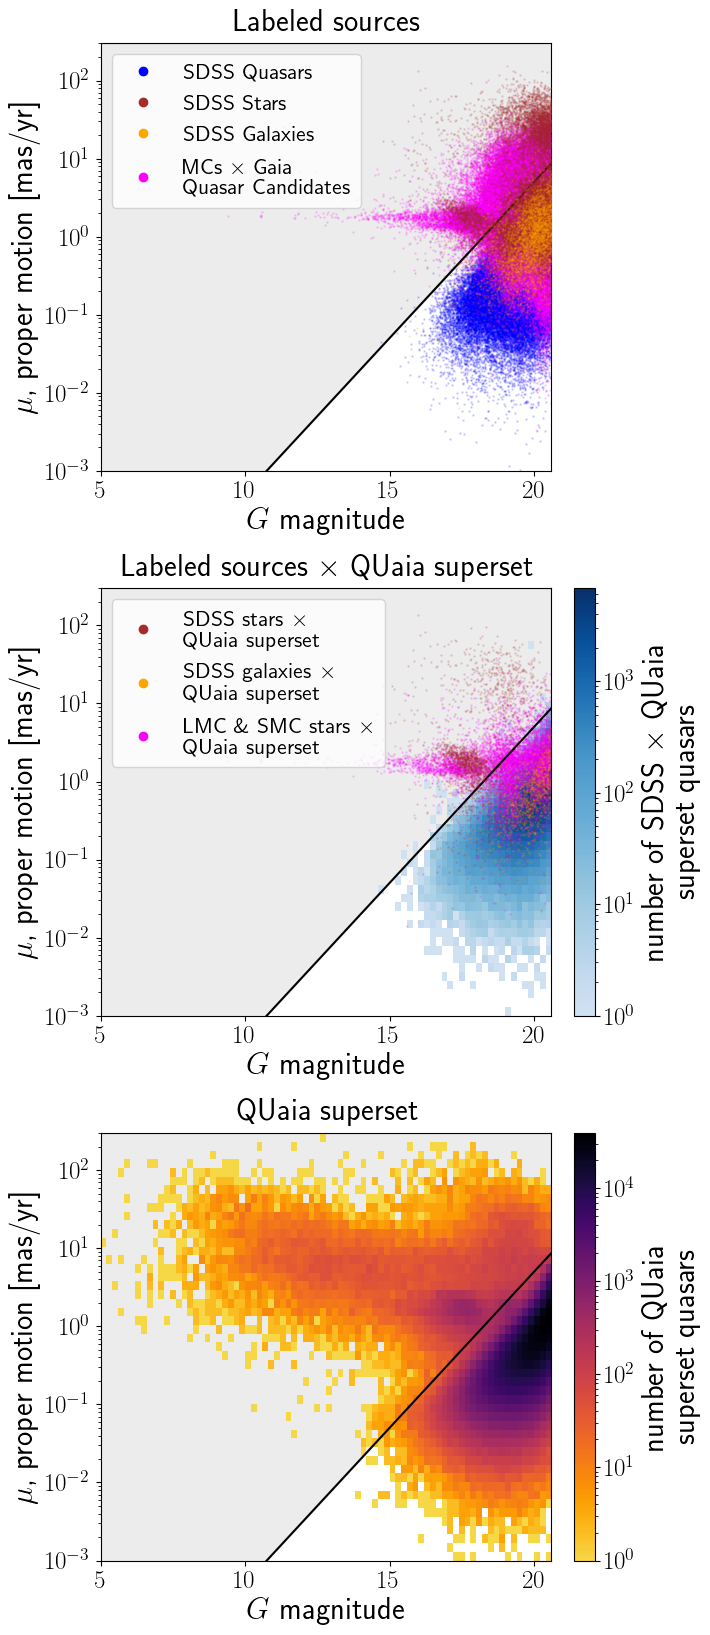
\includegraphics[width=0.42\columnwidth]{G_pm.png}

    \caption{Proper motion $\mu$ vs. $G$ magnitude  for two different sets of sources. The black line shows the cut we make; the shaded gray region is excluded from the catalog. \emph{Top:} The sources for which we have labels (\SDSS data as well as sources near the LMC and SMC in the \emph{Gaia} quasar candidates sample) that are also in the \cat superset (\Gaia DR3 quasar candidates that have all necessary photometry, \Gaia redshift estimates, and $G<\Gmax$). \emph{Middle:} Sources in the top row that are also in the \cat superset (\Gaia DR3 quasar candidates that have all necessary photometry, \Gaia redshift estimates, and $G<\Gmax$). \emph{Bottom:} The superset of quasar candidates from which the \catalog is constructed. The proper motion cut includes nearly all \SDSS quasars in the superset while excluding a large number of stars.} 
    \label{fig:G_pm}
\end{figure}

The full \Gaia quasar candidate sample is known to contain a significant fraction of contaminants (stars and other non-quasars, such as galaxies).
We make an initial cut on proper motion $\mu$, as quasars should have negligible proper motions due to their large distances.
The value of $\mu$ has a dependence on $G$, so we make a cut in this space.
To guide this cut, we use labeled sources: \SDSS quasars, \SDSS galaxies, \SDSS stars, and \Gaia LMC- and SMC-adjacent stars, as described in \S\ref{sec:data_sdss_quasars} and \S\ref{sec:data_contaminants}.
The $G$-$\mu$ distributions of these sources are shown in the top panel of Figure~\ref{fig:G_pm}.
In the middle panel, we show the intersection of these labeled sources with our \cat superset, which consists of sources in the \Gaia quasar candidates table that have \Gaia redshift estimates, complete \Gaia and \unWISE photometry, and are below $G<\Gmax$.
We see that the \SDSS quasars tend to have much smaller proper motions than the other types of sources, with a very linear edge to the $G$-dependence at the high proper motion side of the distribution.
Based on this, we choose the cut
\begin{equation}
    \mu < 10^{0.4\,(G-18.25)} ~.
\end{equation}
At $G=18.25$, this corresponds to $\mu < \sim2.5$, and allows for less harsh cuts at deeper magnitudes given the typically less precise astrometry.
We show this cut overlaid over the \catalog superset in the lower panel of Figure~\ref{fig:G_pm}; based on the labeled data, we can clearly pick out the populations.
The proper motion cut excludes \val{N_removed_pmcut}, $\val{p_removed_pmcut}\%$ of the superset.

\begin{figure*}[p]
    \centering
    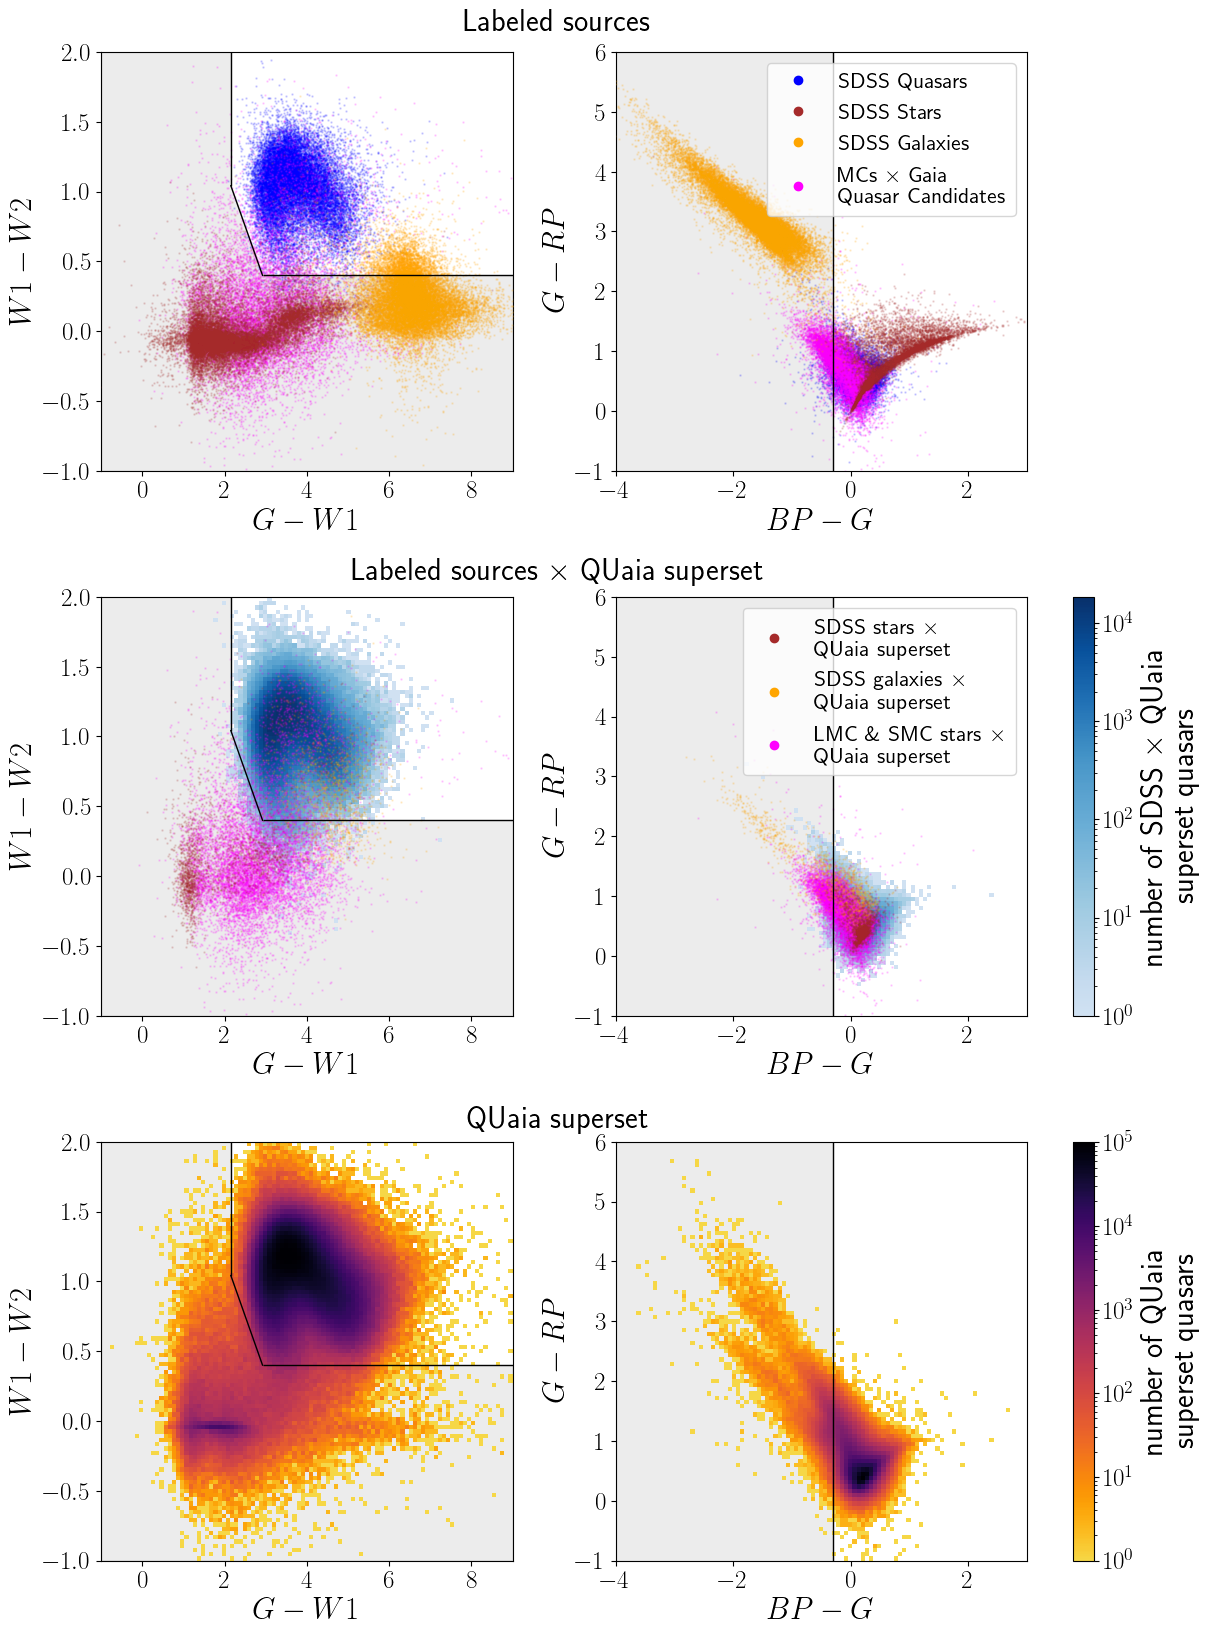
\includegraphics[width=0.8\textwidth]{color_color.png}

    \caption{Color-color plots of three different sets of sources. The left column shows $W1-W2$ vs. $G-W1$ color, and the right column shows $G-RP$ vs. $BP-G$ color. The black lines show the cuts we make; the shaded gray region is excluded from the catalog. The rows have the same samples as in Figure~\ref{fig:G_pm}, except that in the top row only 20,000 of each type of \SDSS source is shown for clarity. In both color-color projections, the labeled sources are mostly localized in particular regions of parameter space, and we can see these populations somewhat clearly in the \cat superset.} 
    \label{fig:color_color}
\end{figure*}

We next determine color cuts based on \Gaia and \unWISE photometry.
Generally, stars and galaxies are dim in redder, IR wavelengths compared to AGN.
For instance, the eBOSS target selection involved a cut in the optical-IR, involving the \SDSS $g$-, $r$-, and $i$-bands and WISE $W1$ and $W2$ bands (as $W3$ and $W4$ have a significant difference in depth) \citep{myers_target_2022}. 

In Figure~\ref{fig:color_color}, we show color-color distributions for the same samples as in Figure~\ref{fig:G_pm}.
The left panel shows $W1-W2$ vs. $G-W1$ color, and the right column shows $G-RP$ vs. $BP-G$ color.
The top row, with the full labeled samples, shows that different types of sources tend to be localized to different areas of this parameter space (we show only a subset of each type for clarity).
In particular, the colors involving \unWISE (left panel) separate out the source types relatively clearly, demonstrating the importance of the \unWISE cross-match: \SDSS quasars have high $W1-W2$ and $G-W1$ color, while galaxies have low $W1-W2$ and high $G-W1$, and stars (both \SDSS stars and stars near the LMC and SMC) are lower in both colors.
In \Gaia color-color space, galaxies tend to have lower $BP-G$ and higher $G-RP$ colors than the other types of sources.
In the middle row of Figure~\ref{fig:color_color}, showing the intersection of the labeled sources with the \cat superset, we see that the superset restrictions have eliminated many of the sources, especially \SDSS galaxies and stars, though a significant number remain.
(We note that it is possible that some of these \SDSS galaxies do host AGN though they weren't classified as such by \SDSS.)
The \cat superset is shown in the bottom panel; we can see clear populations of quasars, stars, and galaxies lining up with the labeled sources.
Importantly, we can see the effect of the stricter \SDSS color selection in the red (high $G-W1$) region of parameter space into which the \Gaia quasar candidates extend, but are not represented in the \SDSS sample in the above panels.

We choose to apply linear cuts in these colors to decontaminate the sample.
While other works (e.g. \citealt{hughes_quasar_2022}) train classifiers to determine which objects are true quasars, we opt for simpler cuts for ease of reproducibility and to avoid imposing the same selection effects as \SDSS, especially as the strict \SDSS color selection may exclude significant regions of quasar parameter space.
We choose four cuts based on the distribution of sources in color-color space. 
The first is in $W1-W2$, which has been shown to be useful for distinguishing quasars; for instance, \cite{nikutta_meaning_2014} demonstrated that a small cross-matched \SDSS quasar sample has high $W1-W2=1.2 \pm 0.16$, while other types of objects---namely star-forming and AGN galaxies, luminous red galaxies and stars---have lower $W1-W2$.
Stars tend to have the lowest $W1-W2$, with a mean of $W1-W2=-0.04 \pm 0.03$, so a cut in $W1-W2$ is a reliable way to filter out stellar contaminants.
We add a cut in $G-W1$ to filter out the bulk of the stars (including the LMC and SMC), and another in $BP-G$ to cut out the galaxy contaminants.
Finally, we find that these single-color cuts were not sufficient to remove all of the LMC and SMC, so we add an additional diagonal cut in $W1-W2$ and $G-W1$, choosing a reasonable slope.

We optimize the values (intercepts) of these four cuts with a grid search, trying values spaced out by 0.1 magnitudes.
We note that while we show the full samples in Figure~\ref{fig:color_color}, in practice we make the proper motion cut before optimizing the color cuts.
We choose that color cuts that maximize our objective function $\mathcal{L}$,
\begin{equation}
    \mathcal{L} = N_\text{q} - \lambda_\text{s} \, N_\text{s} - \lambda_\text{g} \, N_\text{g} - \lambda_\text{m} \, N_\text{m} ~,
\end{equation}
where $N_\text{q}$ is the number of true quasars that make it into the catalog, $N_\text{s}$ \SDSS stars, $N_\text{g}$ \SDSS galaxies, and $N_\text{m}$ LMC and SMC stars, and the $\lambda$ parameters balance the relative ratios of each.
We choose $\lambda_\text{s}=3$, $\lambda_\text{m}=5$, and $\lambda_\text{g}=1$.

The optimal cuts for the objects to keep in the catalog are
\begin{equation}
\begin{split}
    (G-W1) &> 2.15 \\ (W1-W2) &> 0.4 \\ (BP-G) &> -0.3 \\ (G-W1) + 1.2\,(W1-W2) &> 3.4
    %{\colorcutstr} ~.
\end{split}
\end{equation}
These are shown as the black lines in all panels of Figure~\ref{fig:color_color}, with the grey shading indicating exclusion regions.
These cuts, as well as the proper motion cuts described above, exclude ${\sim}\val{p_cut_gsup_gclean}\%$ of the superset, resulting in \val{N_gclean} quasars in our ''decontaminated'' sample.
We apply an additional magnitude cut of $G<\Ghi$ to reduce edge effects in our redshift estimation; this constitutes our deep sample, with \val{N_gcathi} sources.
We refer to this as the \catalog (\cat) in the rest of this work.
However, the catalog becomes less clean and reliable as we push to deeper magnitudes---due to less precise measurements and stronger systematics, notably the \Gaia scanning pattern---so we produce a version of the catalog with $G<\Glo$ to ensure a cleaner sample.
This brighter catalog has \val{N_gcatlo} sources, and we report most of our results on this sample throughout the rest of this work.


\subsection{Spectro-photometric redshifts with \unWISE and \SDSS}
\label{sec:redshifts}

\begin{figure*}
    \centering
    \subfloat[\label{fig:zgaia_zsdss}]{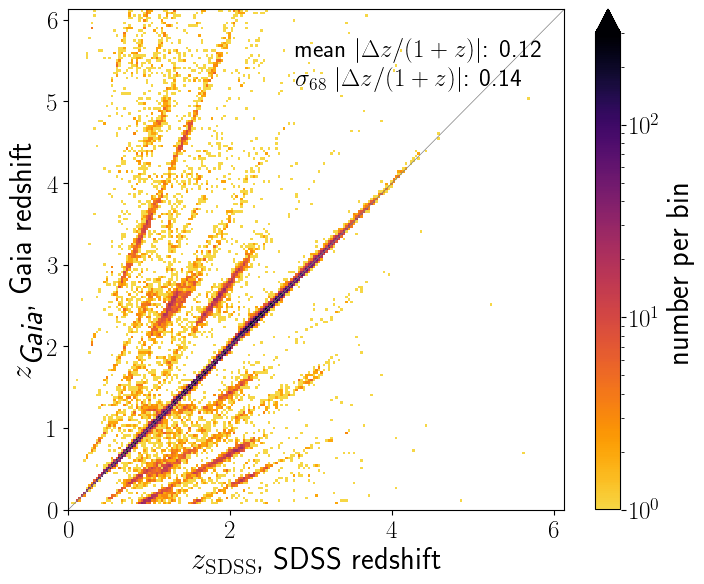
\includegraphics[width=0.45\textwidth]{redshift_zgaia_vs_zdss_Ghi.png}}
    \hspace{5ex}
    \subfloat[\label{fig:zspz_zsdss}] {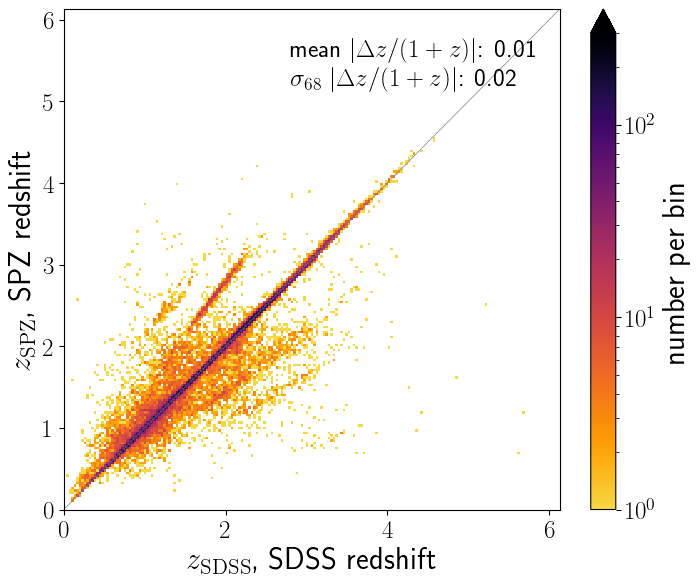
\includegraphics[width=0.45\textwidth]{redshift_zspz_vs_zdss_Ghi.png}}
    \caption{TODO FIX}
    %\caption{(a) \Gaia redshift estimate $\zgaia$ vs. \SDSS (''true'') redshift $\zsdss$ for a test set of sources in our quasar catalog \cat with $G<\Ghi$. (b) Our estimated spectro-photometric (SPZ) redshifts $\zspz$ vs. $\zsdss$ for the same sample. The $\zspz$ redshifts, which are based on a \knn model, significantly decrease both the bias and scatter, as well as catastrophic outliers and unreasonably high redshift estimates. The one-to-one line (perfect accuracy) is shown in grey; note that the color bar is on a log scale, and that a majority of the sources in both cases lie along this line.}
    \label{fig:zsdss_comp}
\end{figure*}

We use \unWISE and \SDSS data to improve the redshift estimation of the sources.
Figure~\ref{fig:zgaia_zsdss} shows the redshifts estimated by the \Gaia QSOC pipeline $\zgaia$ compared to the \SDSS redshifts $\zsdss$ for a test sample of sources from \cat with $G<\Ghi$; note that the 2D histogram is plotted in log-space to show the outliers more clearly.
We find that of the \Gaia redshifts $\zgaia$, $\val{p_acc_zgaia_dzhi_Glo}\%$ ($\val{p_acc_zgaia_dzmid_Glo}\%$) agree to $|\dz|<\val{dzhi}$ ($\val{dzmid}$).
A significant fraction of $\zgaia$ are highly precise: $\val{p_acc_zgaia_dzlo_Glo}\%$ agree with \SDSS to $|\dz|<\val{dzlo}$.
We also clearly see bands of incorrect estimation due to line aliasing issues.
Additionally, in the cross-matched sample, nearly all of the very high $\zgaia$ estimates ($z>4.5$) are shown to be incorrect in comparison to \SDSS.

We train a $k$-Nearest Neighbors (\knn) model to estimate improved redshifts.
(We also tried other models including XGBoost and a multi-layer perceptron, and found that the \knn outperformed both overall.)
We include all sources in our decontaminated catalog (\S\ref{sec:decontam}) which goes out to $G<\Gmax$, in order to have a buffer beyond our desired $G<\Ghi$ sample to reduce edge effects from the training set.
The features that we train on are: the \Gaia redshift $\zgaia$, colors constructed using \Gaia and WISE photometry ($G-RP$, $BP-G$, $BP-RP$, $G-W1$, $W1-W2$), the \Gaia $G$-band magnitude, and the dust reddening $E(B-V)$ at the location of the source.
(We find that including the rest of the photometry does not make a difference in the results.)
The reddening is determined with the \citep{schlafly_measuring_2011} dust map\footnote{The dust map was accessed with the python package \url{https://dustmaps.readthedocs.io}}.
The labels are the \SDSS redshifts, $\zsdss$.

We use as our labeled data sources from the cross-matched \SDSS DR16Q sample (\S\ref{sec:data_sdss_quasars}) that are also in our decontaminated catalog \cat, so that we train on sources drawn from the same distribution to which we will apply the model; this is \val{N_sqclean} sources.
We apply a 70\%/15\%/15\% train/validation/test split.
We build a $k$-d tree on the training set features using the \texttt{KDTree} implementation of \texttt{sklearn}.
At the prediction stage, we access the $K$ nearest neighbors of each input feature vector, first excluding neighbors with zero distance in feature-space (i.e. neighbors that are in the training set).
We assign the predicted label to be the median $\zsdss$ of the $K$ nearest neighbors, and the uncertainty to be the symmetrized inner 68\% error of those neighbors.
We use the validation set to tune $K$, and choose the value that maximizes the fraction of predicted redshifts with $|\dz|<\val{dzmid}$, which is $K=27$; we note that this value only varies at the $\sim$1\% level for values $15 < K < 50$, and is similar for other choices of $|\dz|$. 
Finally, we apply the model to the full \cat and output \knn redshift estimates, $\zknn$, for each source.

\begin{figure}
    \centering
    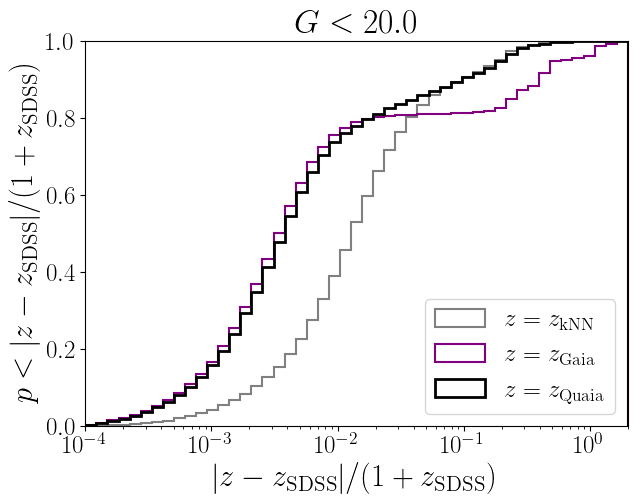
\includegraphics[width=0.55\columnwidth]{redshift_error_cumulative_Glo.png}
    \caption{TODO FIX}
    %\caption{The cumulative distribution of redshift errors for \cat test set sources with $G<\Glo$, considering \SDSS spectroscopic redshifts $\zsdss$ as ground truth, for estimates directly from our \knn model (grey), the original $\zgaia$ redshifts (purple), and our final $\zspz$ estimates (black) based on a combination of the other two. Our SPZ redshifts have far fewer outliers and similar precision compared to the \Gaia estimates.}
    \label{fig:z_error_cumulative}
\end{figure}

The results are shown in Figure~\ref{fig:z_error_cumulative}, which shows the cumulative distribution of errors $|\dz|$ for $\zknn$ compared to that of $\zgaia$ (with $\zsdss$ as the truth) for the test set with $G<\Glo$.
(The shapes are similar for $G<\Ghi$, just shifted to somewhat lower accuracy.)
We find that the $\zknn$ estimates have far fewer outliers than $\zgaia$.
However, the $\zgaia$ estimates tend to be more precise, as they use the full spectral information, while the \knn is essentially smoothing over the likeliest neighboring sources in feature space. 
We thus choose to combine the properties of both of these redshift estimates to obtain our final \emph{spectro-photometric} (SPZ) redshifts $\zspz$ in the following way.
For sources for which $\zspz$ and $\zgaia$ agree to $|\dz|<0.05$, we assign $\zspz = \zgaia$ to preserve the precision of the \Gaia estimate.
For sources for which $\zspz$ and $\zgaia$ differ by $|\dz|>0.1$, we assign $\zspz = \zknn$ to preserve accuracy.
In between these thresholds, we apply a smooth, linear transition to avoid hard features in our estimates.
These $\zspz$ estimates are also shown in Figure~\ref{fig:z_error_cumulative} compared to the ''true'' \SDSS redshifts, and we can see that these achieve nearly as high precision as $\zgaia$ while maintaining the high accuracy of $\zknn$.

Our $\zspz$ results for the test set are shown in Figure~\ref{fig:zspz_zsdss} compared to $\zsdss$, here shown for the full catalog depth $G<\Ghi$. 
We find that $\val{p_acc_zspz_dzhi_Ghi}\%$ ($\val{p_acc_zspz_dzmid_Ghi}\%$) of our SPZ redshifts agree to $|\dz|<\val{dzhi}$ $(\val{dzmid})$, and $\val{p_acc_zgaia_dzlo_Ghi}\%$ highly agree to $|\dz|<\val{dzlo}$.
We also give the mean and uncertainty of $|\dz|$ in the figure; our SPZ redshifts significantly decrease the bias and scatter.
The SPZ estimation corrected all of the very high-$z$ \Gaia estimates, and some of the intermediate-outlying aliasing effects.
We still have some catastrophic outliers due to line aliasing, but with our SPZ redshifts we find a reduction in the number of $|\dz|>\val{dzhi}$ (\val{dzmid}) outliers by \val{factor_reduction_outliers_dzhi_Ghi} (\val{factor_reduction_outliers_dzmid_Ghi}) compared to the \Gaia redshift estimates.


\begin{figure}
    \centering
    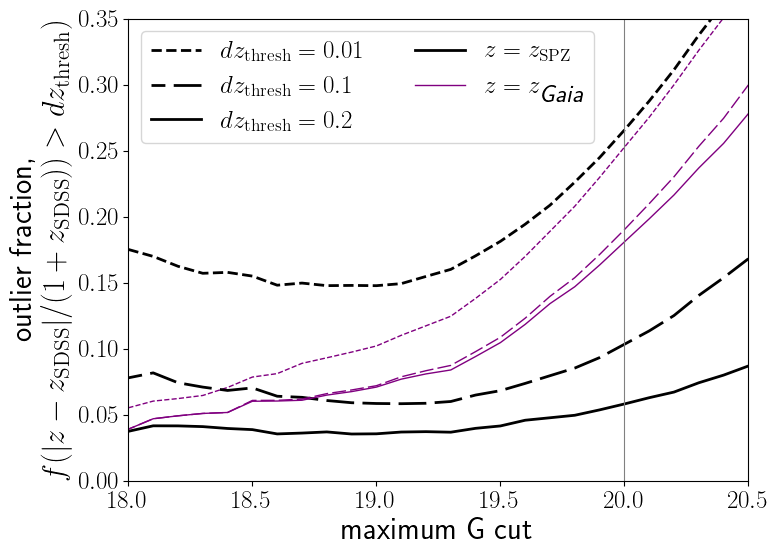
\includegraphics[width=0.55\columnwidth]{redshift_outliers_vs_Gmax.png}
    \caption{TODO FIX}
    %\caption{The fraction of outlying redshifts with $|\dz| > (\val{dzlo}, \val{dzmid}, \val{dzhi})$, as a function of $G$ magnitude, for our redshift estimation test set. The SPZ redshifts are shown in black, and the \Gaia redshifts in purple. The fraction of outliers increases steeply with increasing $G$ for $G>19.5$ for both $\zspz$ and $\zgaia$, though the fraction of catastrophic outliers for $\zspz$ is significantly lower (and the dependence less steep) compared to $\zgaia$.}
    \label{fig:z_G_dep}
\end{figure}

We investigate the dependence of the redshift error on $G$-band magnitude in Figure~\ref{fig:z_G_dep}.
The fraction of redshifts with an error above a various thresholds is shown as a function of samples with given cut on $G$.
The errors are lowest at a bright magnitude cut of $G < \sim$$\val{Gbright}$; in this sample, sources with SPZ redshift estimates inaccurate to $|\dz|>\val{dzhi}$ (\val{dzmid}) comprise only $\val{p_outliers_zspz_dzhi_Gbright}\%$ ($\val{p_outliers_zspz_dzmid_Gbright}\%$) of the sample, and to the more stringent requirement of $|\dz|>\val{dzlo}$, $\val{p_outliers_zspz_dzlo_Gbright}\%$.
This outlier fraction increases steadily as fainter sources are included.
For $G<\Glo$, $\val{p_outliers_zspz_dzhi_Glo}\%$ ($\val{p_outliers_zspz_dzmid_Glo}\%$) are inaccurate to $|\dz|>\val{dzhi}$ $(\val{dzmid})$, and $\val{p_outliers_zspz_dzlo_Glo}\%$ for $|\dz|>\val{dzlo}$.
Compared to the \Gaia redshift estimates, the SPZ estimates $\zspz$ reduce the number of $|\dz|>\val{dzhi}$ (\val{dzmid}) outliers by \val{factor_reduction_outliers_dzhi_Glo} (\val{factor_reduction_outliers_dzmid_Glo}).
The choice of $G$ cut to use in a given analysis will depend on the nature of the analysis and its sensitivity to outliers. 
We also find that the fraction of errors increases slightly towards very bright magnitude cuts.
As this only occurs for our $\zspz$ and not the $\zgaia$ estimates, we speculate that this is due to low number statistics in the bright regime that lead to a low number of nearby neighbors in the \knn and thus poorer estimates.


\subsection{Selection Function Modeling}
\label{sec:selfunc_methods}

\begin{figure*}
    \centering

    \subfloat[\label{fig:systematics_dust}]{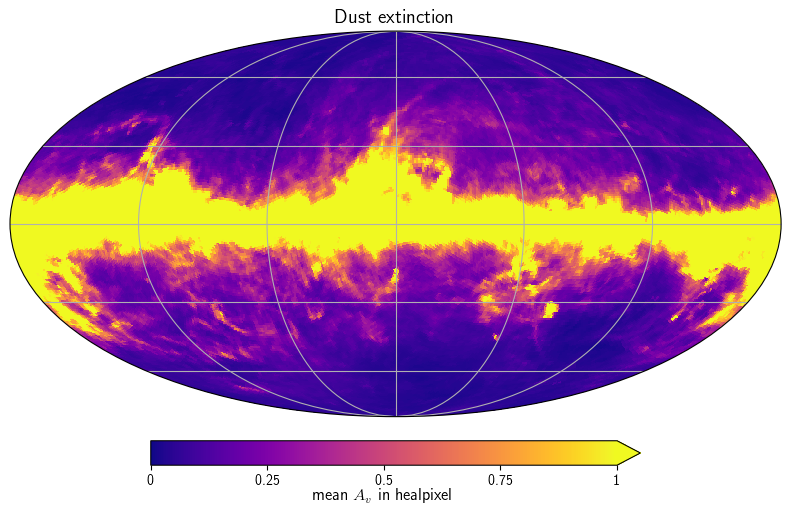
\includegraphics[width=0.45\textwidth]{systematics_map_dust.png}}
    \hspace{5ex}
    \subfloat[\label{fig:systematics_stars}]{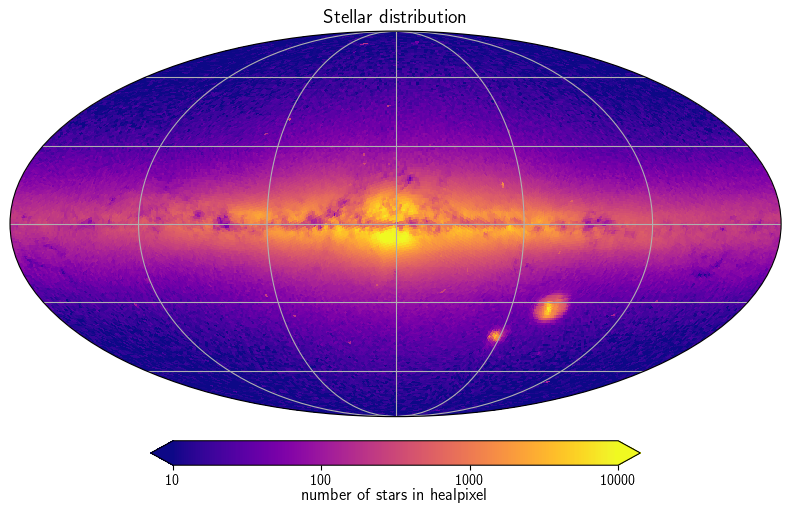
\includegraphics[width=0.45\textwidth]{systematics_map_stars.png}}
    
    \subfloat[\label{fig:systematics_mcs}]{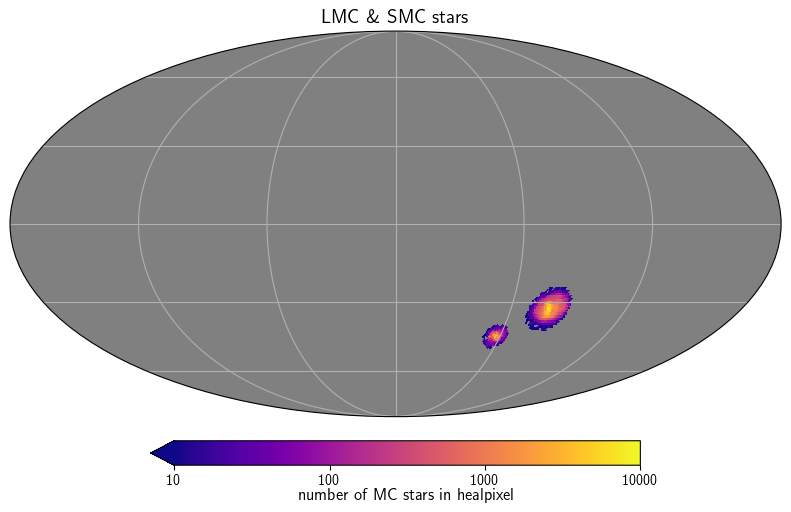
\includegraphics[width=0.45\textwidth]{systematics_map_mcs.png}}
    \hspace{5ex}    
    \subfloat[\label{fig:systematics_m10}]{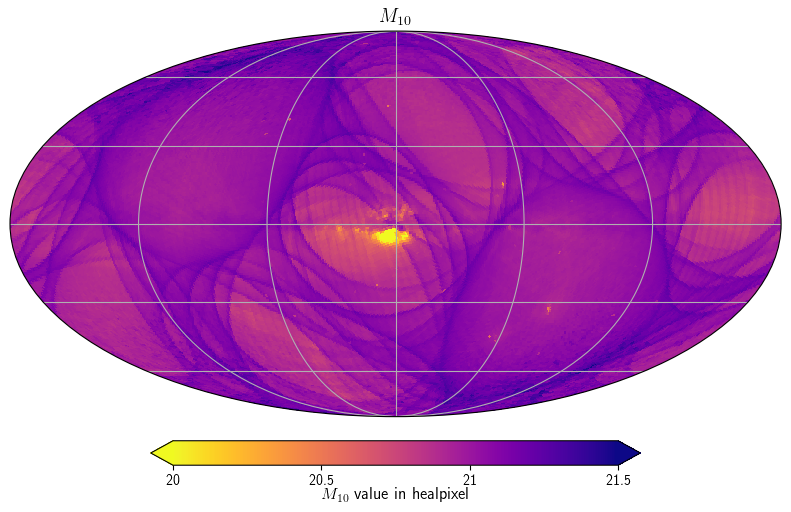
\includegraphics[width=0.45\textwidth]{systematics_map_m10.png}}

    \caption{The systematics maps used in the selection function model: (a) dust extinction based on \cite{schlafly_measuring_2011}; (b) the stellar distribution based on $\sim$10.6 million randomly selected \Gaia sources with $18.5 < G < 20$; (c) stars from the above panel belonging to the LMC and SMC, with the background subtracted; and (d) the quantity $M_{10}$, the median magnitude of sources with at least 10 \Gaia transits, which encodes the scanning law and source crowding. Note that the color bar on the $M_{10}$ map is reversed, as high $M_{10}$ indicates a cleaner region, the inverse of the other maps.}
    \label{fig:systematics}
\end{figure*}

Observational and astrophysical effects impact which sources we observe and their properties; this is known as the selection function. 
As \Gaia is a space-based mission, it avoids many of the observational issues of ground-based surveys, such as seeing and airmass.
However, there are still significant selection effects: for our model, we consider dust, stellar density, and the \Gaia scan pattern.

We fit a selection function model to a particular version of the catalog, namely a particular maximum $G$.
We make a healpix map of the catalog with NSIDE=64 and count the number of observed catalog sources in each healpix pixel.
In the case of no selection effects (and under the assumption of isotropy), we would expect each pixel to contain roughly the same number of sources.
Our goal is to model the dependence between the number of sources per pixel and the various systematics.

The systematics maps (templates) we use are shown in Figure~\ref{fig:systematics}. 
We use the dust map of \cite{schlafly_measuring_2011}, and convert it to a healpix map of NSIDE=64.
To do this, we evaluate the reddening $E(B-V)$ at the centers of pixels of a high-resolution NSIDE=2048 healpixelization of the sphere.
We convert these to extinction values by multiplying by $R_V=3.1$, and then take the mean of all of these values within each healpixel target NSIDE=64 map.
This produces a smoothed dust extinction map on the desired scale.
The result is shown in Figure~\ref{fig:systematics_dust}; the extinction is highest around the galactic plane, with structure extending outwards.

For the stellar distribution, we randomly select $\sim$10.6 million \Gaia sources with $18.5<G<20$, the magnitude range of most of our quasar sample.
The vast majority of these will be true stars (though they will contain some other types of objects).
We count the number of stars per NSIDE=64 pixel; this is shown in Figure~\ref{fig:systematics_stars}.
We find that we require a separate map of the LMC and SMC to properly fit these regions, suggesting that the quasar catalog has a different dependence on the MCs than the galactic plane stellar distribution.
To do this we cut out a wide region around each MC (9 degrees in radius around the LMC and 5 around the SMC), and subtract the background, which we approximate using the horizontally mirrored region of the stellar distribution map.
This is shown in Figure~\ref{fig:systematics_mcs}.

For the \Gaia completeness, we use the quantity $M_{10}$ introduced by \cite{cantat-gaudin_empirical_2023}\footnote{This map can be accessed with the \texttt{gaiaunlimited} package, \url{https://gaiaunlimited.readthedocs.io}}.
$M_{10}$ is the median magnitude in a given sky patch of the \Gaia sources with at least 10 transits across the \Gaia field of view; it incorporates the effects of both the scanning law and source crowding.
The actual completeness map derived by \cite{cantat-gaudin_empirical_2023} depends on both $M_{10}$ and $G$-band magnitude; however, this completeness is still extremely close to 1 for nearly all of the sky for $G=\Glo$, the limiting magnitude of our clean quasar catalog, due to the differences in the selection function and magnitude dependence for stars compared to quasars.
Thus we cannot use the completeness map directly, but we do still expect a dependence of the quasar selection function on the \Gaia scanning law, so use the $M_{10}$ map directly to capture this effect.
We down-sampled the map to NSIDE=64; this is shown in Figure~\ref{fig:systematics_m10}.


To model the selection function we use a Gaussian process, a flexible machine learning method for regression; for a detailed treatment, see \cite{RasmussenWilliams2006}.
(We first tried a linear model and found that it gave a very poor fit, as there are significant nonlinearities between the systematics and the catalog number density.)
We first scale the data: for the labels (number of \cat sources per pixel) we work in their logarithm, and only fit for the pixels with a nonzero number of sources.
For the stellar distribution and MC map templates, we also take the log of the number of quasars per pixel; for the MC map we first replace zeros with a very small value.
For all of the input feature maps, we take the mean-subtracted systematics values in order to use a zero-mean Gaussian process.
We assume a Poisson error on the labels (and apply the appropriate log transformation).
For the Gaussian process, we use the \texttt{george} software package \citep{Ambikasaran2016}. 
We use an exponential squared kernel $k$ of the form
\begin{equation}
    k(r^2) = \text{exp}\left(\frac{-r^2}{2}\right)~,
\end{equation}
where $r$ is the distance between points in feature space.
We train the Gaussian process on all of the data, optimizing the parameter vector using the BFGS solver.
We finally evaluate the predicted number of sources in each pixel.
Where there were no \cat sources in the label map, we fix the prediction to zero.

To convert this to a selection function in terms of the probability of inclusion of a source in the final catalog, we first identify ``clean'' pixels in the map having low dust extinction ($A_v < 0.03$), low star counts ($N_\mathrm{stars} < 15$), no MC stars, and high $M_{10}$ ($M_{10} > 21$); this results in 301 pixels.
We take the mean predicted number of quasars in these clean pixels, normalize the predicted source numbers by this mean, and then fix pixels with normalized values greater than 1 to exactly 1.
The result is a selection function map in terms of the probability of a source's inclusion in the catalog.
This fit must be done for each version of the catalog as it depends on the particular number density and distribution of sources, which depends most notably on magnitude.


\section{The Catalog: Results and Verification}
\label{sec:catalog}

\subsection{Properties of the catalog}
\label{sec:properties}

\begin{figure*}
    \centering
    \subfloat[\label{fig:gcatlo_2d}]{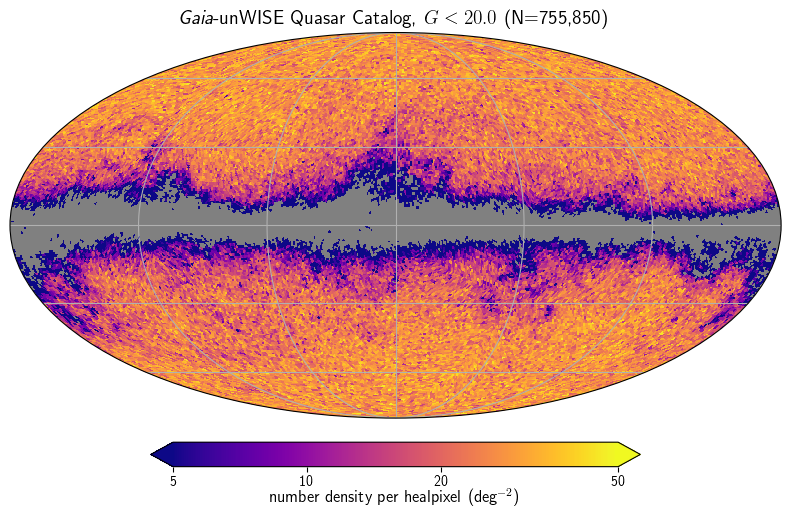
\includegraphics[width=0.8\textwidth]{gcatlo_2d.png}}
    
    \subfloat[\label{fig:gcathi_2d}]{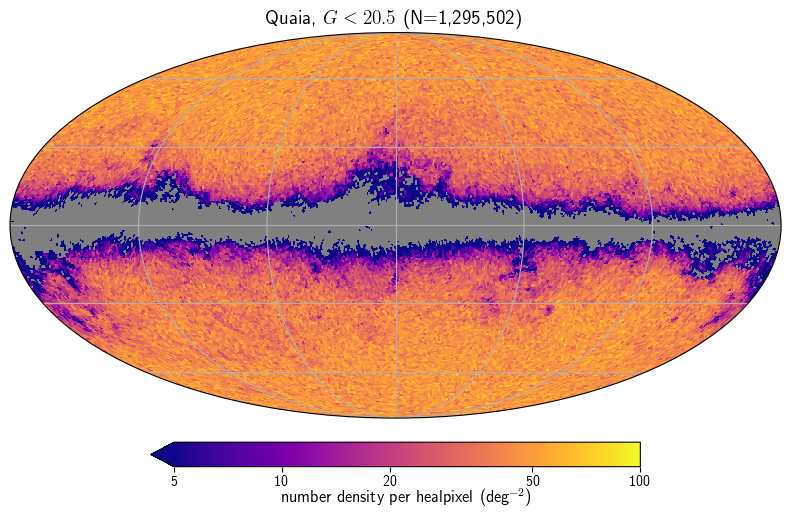
\includegraphics[width=0.8\textwidth]{gcathi_2d.png}}
    \caption{TODO FIX}
    %\caption{Sky distribution of our \catalog, in Galactic coordinates and displayed using a Mollweide projection. Panel (a) shows sources with $G<\Glo$, the cleaner version with more reliable redshifts, and (b) shows the catalog down to its magnitude limit of $G<\Ghi$.}
    \label{fig:gcat_2d}
\end{figure*}

Our \catalog consists of \val{N_gcatlo} (\val{N_gcathi}) quasar candidates with $G<\Glo$ $(\Ghi)$.
The sky distribution of \cat for each of these magnitude limits is shown in Figure~\ref{fig:gcat_2d}.
The catalog covers the full sky, besides the galactic plane, including the Southern sky---most of which is not well covered by other surveys (see the bottom panels of Figure~\ref{fig:2d_comp}, discussed further in \S\ref{sec:comparison}). 
The sky distribution is remarkably uniform, and the non-uniform imprints visually follow the selection effects that we incorporated into our selection function map, most notably the dust distribution (Figure~\ref{fig:systematics_dust}). 
\cat also does not show an obvious overdensity around the LMC and SMC (as the \Gaia purer sample does), as we have removed these with our decontamination procedure.
In fact, there is now a slight underdensity of sources near the LMC; this makes sense as some quasars in that sky region would be as they are blocked by the LMC, though it is possible we have somewhat over-corrected for this and removed some true quasars. 

The dearth of quasars in the galactic plane is due largely to dust extinction and stellar crowding, as well as the fact that the \SDSS training set quasars (for both the original \Gaia DR3 quasar candidates sample and our decontamination procedure) are not representative of quasars in this dust-reddened region. 
If we exclude the regions with very high extinction $A_v>\val{Avhi}$, the quasars nearly uniformly cover the remaining sky area which comprises \val{area_below_Avhi} ($f_\text{sky}=\val{fsky_below_Avhi}$).
This results in an effective volume of \val{volume_effective_gcathi_below_Avhi} (\val{volume_effective_gcatlo_below_Avhi}) for the $G<\Ghi$ ($G<\Glo$) sample, which takes into account the number density distribution as a function of redshift.
In comparison, \SDSS DR16Q---the largest existing spectroscopic quasar sample---has \val{N_sqall} sources with reliable redshifts, covers \val{area_sdss} ($f_\text{sky}=\val{fsky_sdss}$), and has an effective volume of \val{volume_effective_sdss}.
The \catalog thus covers a significantly larger area, and correspondingly larger volume, than the \SDSS quasar sample by a factor of \val{factor_area_belowAvhi_sdss}.
Despite its lower number density, the $G<\Ghi$ \cat still spans a somewhat larger effective volume than \SDSS by a factor of \val{factor_volume_effective_gcathi_sdss}.

\begin{figure*}
    \centering

    \subfloat[\label{fig:gcathi_3d}]{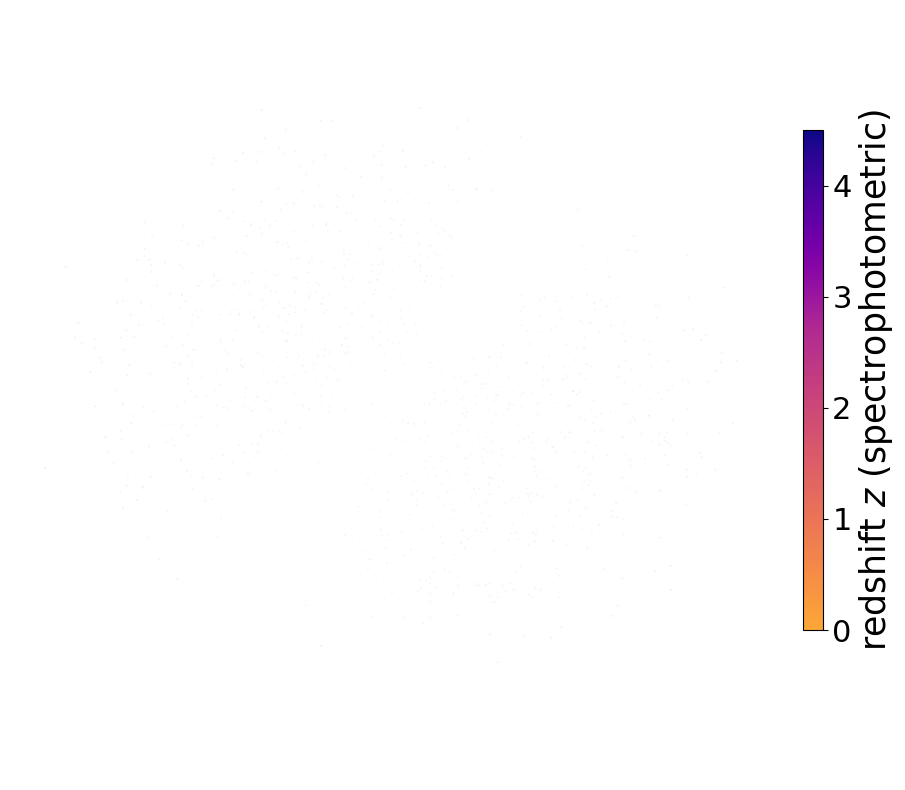
\includegraphics[width=0.48\textwidth]{gcathi_3d.png}}
    \hspace{1em}
    \subfloat[\label{fig:sdss_3d}]{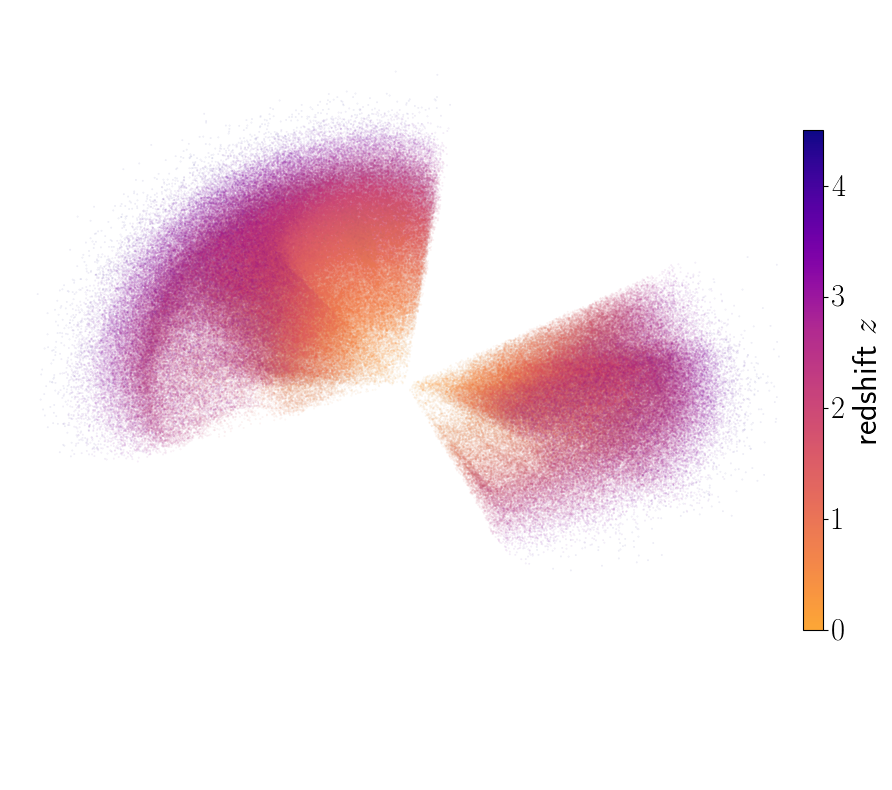
\includegraphics[width=0.48\textwidth]{sdss_3d.png}}

    \caption{(a) A 3D projection of the \catalog. (b) The same projection for the quasars in \SDSS DR16Q. The colorbar shows the redshifts of the quasars ($\zspz$ for \cat, $\zgaia$ for \SDSS). \cat spans a larger volume and has a cleaner selection function than the \SDSS sample. \emph{An animated version is available at} \url{https://cosmo.nyu.edu/ksf/QSOs.gif}.}
    \label{fig:3d}
\end{figure*}

We show a 3D projection of the \cat catalog in Figure~\ref{fig:gcathi_3d}, using our $\zspz$ redshift estimates converted to spatial coordinates with a fiducial Planck cosmology.
Figure~\ref{fig:sdss_3d} shows the \SDSS quasar sample for comparison.
The \catalog spans a much larger volume than \SDSS, and also has a cleaner selection function; the distribution looks homogeneous in 3D, while strong spatial selection effects can be seen in the \SDSS sample.

\begin{figure*}
    \centering
    \includegraphics[width=0.9\textwidth]{redshift_dists_Glo.png}
    \caption{TODO FIX}
    %\caption{Redshift distribution of the $G<\Glo$ \catalog for our spectro-photometric redshift estimates $\zspz$ (black), normalized to the total number of objects. For comparison we also show the normalized distributions of the \Gaia redshift estimates $\zgaia$ for the same \cat sources (purple); $\zgaia$ for the sources in the full \Gaia quasar candidate sample (grey); $\zgaia$ for the \Gaia DR3 ''purer'' subsample (green); and the \SDSS redshifts $\zsdss$ for the \SDSS DR16Q quasar sample (blue). All distributions are shown for $G<\Glo$ subsamples for clear comparison. The median redshift of each distribution is shown by the diamond and vertical line in the respective color.} 
    \label{fig:z_dists}
\end{figure*}

We show the redshift distribution of \cat in Figure~\ref{fig:z_dists}.
The distribution of our \Gaia--\unWISE--\SDSS spectro-photometric redshift estimates, $\zspz$, for the catalog down to $G<\Glo$ is shown in black.
We compare this to other samples cut to the same $G$ limit: the \Gaia redshifts $\zgaia$ for the same sample; $\zgaia$ for the all sources in the \Gaia quasar candidates sample (that have redshift  estimates); $\zgaia$ for sources in the purer \Gaia sample; and $\zsdss$ for the \SDSS DR16Q sources.
We see that the SPZ redshifts have a smoother distribution than the others, with a clear peak around $z=1.5$; the median value is \val{zmed_gcatlo}.
These SPZ estimates have also greatly reduced the high-$z$ tail present in the \Gaia redshifts.
There are still a significant amount of intermediate-$z$ objects; $\val{p_above_zintermediate_gcatlo}\%$ ($N=\val{N_above_zintermediate_gcatlo}$) of the sources in the $G<\Glo$ catalog have $z>\val{zintermediate}$.
We note that the $\zgaia$ redshift distribution for the purer sample is very similar to those same redshift estimates for \cat; this is partially because a very high fraction of the objects in \cat are also in the larger \Gaia purer sample (see Figure~\ref{fig:frac_matrix}).
We also see a slight bump in the $\zspz$ distribution around $z\sim2.25$, the same location as the peak in the \SDSS DR16Q quasar distribution.
This indicates that features in the training sample have been imprinted onto our redshift model, though the distortion is quite slight.

\begin{figure}
    \centering
    \includegraphics[width=0.6\columnwidth]{G_dist}
    \caption{Distribution of $G$ magnitudes of \cat (black), compared to the full \Gaia candidates sample (grey), the {\Gaia} 'purer' sample (green), and the \SDSS DR16Q quasar sample (blue).}
    \label{fig:G_dist}
\end{figure}

We show the $G$-band magnitude distribution of \cat is shown in Figure~\ref{fig:G_dist}, in comparison the other \Gaia and \SDSS quasar samples described above.
We see that our catalog (as well as the \Gaia 'purer' sample) has removed all of the sources with excessively bright (for quasars) magnitudes $G<12.5$ that are present in the full \Gaia sample, as well as many sources with $12.5<G<16$.
For the \Gaia DR3 and \SDSS samples, the number of quasars drops off sharply after $G\sim20.75$; to avoid the complicated selection effects at these depths, we limit our catalog to $G<\Ghi$ as shown.
We also note that the \SDSS DR16 quasars do not extend as bright as \cat, and this extrapolation past the training set could bias the results in this regime, though in practice this affects very few sources.


\subsection{The selection function model}
\label{sec:selfunc}

\begin{figure}
    \centering
    \subfloat[\label{fig:selection_function_map}]{\includegraphics[width=0.75\columnwidth]{selection_function_Glo.png}}
    \vspace{0.1ex}
    \subfloat[\label{fig:selection_function_residuals}]{\includegraphics[width=0.75\columnwidth]{residuals_Glo.png}}
    \caption{TODO FIX}
    %\caption{(a) The selection function map for the $G<\Glo$ \catalog, based on a Gaussian process model of the dust, stellar distribution, and $M_{10}$. (b) The fractional residuals between a random catalog down-sampled by the modeled selection function and the true $G<\Glo$ \catalog.}
    \label{fig:selection_function}
\end{figure}

We show the results of our selection function modeling (\S\ref{sec:selfunc_methods}) for the $G<\Glo$ catalog in Figure~\ref{fig:selection_function}.
The selection function map is shown in Figure~\ref{fig:selection_function_map}: the relationship to the dust and stellar distribution maps is clear visually.
In Figure~\ref{fig:selection_function_residuals}, we show the residuals between a random catalog down-sampled by this selection function and the true quasar catalog.
The residuals generally look like homogenous noise, indicating a good fit; the root mean squared fractional error is \val{rmse_fractional_residuals_Glo}.
Around the edges of the galactic plane the random is over-predicted, meaning the completeness there was predicted to be higher than it actually is; this could indicate that our templates are not fully capturing the selection effects.
This issue could be circumvented by applying a latitude cut for sensitive analyses.
The selection function map for the $G<\Ghi$ catalog (not shown) is also provided as a data product, as well as the code to fit the selection function for any other subsample of the catalog.


\subsection{Comparison to existing quasar catalogs}
\label{sec:comparison}

\begin{figure*}
    \centering

    \subfloat[\label{fig:2d_gpurer_Ghi}]{\includegraphics[width=0.45\textwidth]{gpurer_Ghi_2d.png}}
    \hspace{5ex}
    \subfloat[\label{fig:2d_milliquas}]{\includegraphics[width=0.45\textwidth]{milliquas_Ghi_2d.png}}

    \subfloat[\label{fig:2d_sdss}]{\includegraphics[width=0.45\textwidth]{sdss_Ghi_2d.png}}
    \hspace{5ex}
    \subfloat[\label{fig:2d_wiseps}]{\includegraphics[width=0.45\textwidth]{wiseps_Ghi_2d.png}}
    \caption{TODO FIX}
    %\caption{Other current quasar catalogs for comparison with our \catalog. All are shown for sources with $G<\Ghi$ or the equivalent converted from another band, in galactic coordinates and displayed using a Mollweide projection. The catalogs are: (a) the \Gaia DR3 'purer' sample, (b) the Milliquas catalog, (c) the \SDSS DR16Q sample, and (d) the WISE-PS1-STRM catalog. Note that the color bars have different scales in each panel.}
    \label{fig:2d_comp}
\end{figure*}

We compare the \catalog to other existing quasar catalogs: 
Projections of these catalogs are shown in Figure~\ref{fig:2d_comp}. 
We show the \Gaia purer sample (Figure~\ref{fig:2d_gpurer_Ghi}); Milliquas, a meta-catalog compiling confirmed quasars from the literature (Figure~\ref{fig:2d_milliquas}); \SDSS, the current best spectroscopic sample (Figure~\ref{fig:2d_sdss}); and a cross-matched catalog of WISE and Pan-STARRS (WISE-PS1), the current best large-area photometric redshift quasar sample (Figure~\ref{fig:2d_wiseps}).

The \Gaia purer sample is described in \S\ref{sec:data_gaia}; here we include only sources with QSOC redshift estimates ($\zgaia$).
The Milliquas catalog was compiled by \cite{flesch_million_2021}; a significant portion of the sources are from \SDSS and \textsl{AllWISE}.
The \SDSS catalog is the one detailed in \S\ref{sec:data_sdss_quasars}.
The WISE-PS1 sample was constructed by \cite{beck_wise-ps1-strm_2022}, based on the Source Types and Redshifts with Machine learning (STRM) algorithm by \cite{beck_ps1-strm_2020}.
The quasar catalog with updated photometric redshifts is presented by \cite{kunsagi-mate_photometric_2022}; here we include only those quasars with redshifts labeled ''reliable'', which is $\val{p_reliable_wiseps}\%$ of the sample.
For each of these samples, we have shown quasars brighter than a limiting magnitude of $G\sim\Ghi$; for the non-\Gaia catalogs we convert to $G$ from the survey's $r$-band magnitude using the conversion in equation (2) of \cite{proft_exploration_2015}, which is based on the \SDSS $r'$ band.
While this should give a reasonable estimate for the \SDSS sample (using $r_\text{SDSS}$) and the WISE-PS1 sample (using $r_\text{PS1}$ which is very similar to $r_\text{SDSS}$), it may not be as reliable for Milliquas which catalogs ''red'' magnitudes from various sources, as well as for sources with $z>3$ which were not included in the \cite{proft_exploration_2015} fit.

\begin{table*}
    \centering
    \caption{A comparison between quasar catalogs, showing the number of sources N, the fraction of sky covered $f_\mathrm{sky}$, the effective volume $V_\mathrm{eff}$, the number density $\bar{n}$, the median redshift $z_\mathrm{med}$, and the fraction of sources with a redshift error less than 0.2 and 0.01.}
    \begin{tabular}{| c | c | c | c | c | c | c | c |}
    \hline
     & N & $f_\mathrm{sky}$ & $V_\mathrm{eff}$ & $\bar{n}$ & $z_\mathrm{med}$ & $f(|\dz|<0.01)$ & $f(|\dz|<0.2)$ \\ 
     \hline
     \Gaia cosmo & & & & & & & \\  
     \hline
     \Gaia purer & & & & & & & \\
     \hline
     Milliquas & & & & & & & \\
     \hline
     \SDSS & & & & & & & \\
     \hline
     WISE-PS1 & & & & & & & \\
     \hline
    \end{tabular}
    \label{tab:catalog_comp}
\end{table*}

A summary of the catalogs is shown in Table~\ref{tab:catalog_comp}, for the $G<\sim$\Ghi subsamples.
Compared to the \Gaia purer sample, the \catalog has a smaller number of objects and a significantly higher fraction of good redshifts.
The Milliquas catalog contains \val{N_mill} sources, fewer than \cat, and is very heterogeneous across the sky, so we don't include coverage and number density information; the redshifts are also heterogeneous, but we show statistics to give an idea. 
\cat is similar in number to the \SDSS sample, but covers a factor of XXX more sky area.
The photometric catalog WISE-PS1 covers about 3/4 of the sky (limited by Pan-STARRS); the \Gaia DR3 quasar sample is the only survey that covers the entire sky and has reliable redshift information.
\cat contains the largest number of sources with $G<\Ghi$ of any of these catalogs, though WISE-PS1 comes very close, and the other catalogs do go deeper, with varying levels of reliability at those faint magnitudes.
The WISE-PS1 sources have photometric redshifts which are substantially worse than our \Gaia catalog: only XXX\% of the WISE-PS1 sources have $|\dz|<0.2$ (with respect to \SDSS), compared to XXX\% of \Gaia sources.

We also note that the ongoing DESI survey \citep{Aghamousa2016} will observe a high density of quasars over a large sky area \citep{yeche_preliminary_2020}, which will be competitive with and complementary to this \Gaia--\unWISE catalog.


\subsection{Catalog format}
\label{sec:format}

\begin{table*}
    \caption{The format and column descriptions of the \catalog, published as a FITS data file. For the example entry, we show the first catalog row that has values for all of the columns.}
    \centering
    \input{data/data_quaia/catalog_table.txt}
    \label{tab:catalog}
\end{table*}

The \catalog contains our decontaminated quasar sample with computed redshift information, relevant \Gaia properties, and cross-matched catalog information.
The complete catalog format with column names, units, column descriptions, and an example entry, are shown in Table~\ref{tab:catalog}.
Additional information for the sources can be obtained by joining the catalog with the relevant data source with the associated identifier (\Gaia or \unWISE).
We include only sources with $G<\Ghi$ in the catalog; we also publish a version limited to $G<\Glo$, along with the selection function models fit to each (\S\ref{sec:selfunc}) and ''random'' catalogs generated from the selection functions.
The catalog includes our SPZ redshifts $\zgaia$ along with redshift errors $\sigma_{z\mathrm{SPZ}}$, sky position, \Gaia photometry, \unWISE photometry, and proper motion information.
The catalog is in FITS format, and units and descriptions are provided for each column.
% For quasars in our catalog that have an \SDSS match, we include the \SDSS source ID and the \SDSS spectroscopic redshift.
% We also include a flag for whether the quasar was included in the \Gaia purer sample.


\subsection{Potential applications}
\label{sec:applications}

The \catalog has many potential applications.
The immense volume of quasars, which are highly biased cosmic web tracers, lends itself to large-scale structure analyses.
It is particularly well-suited to cross-correlations with other all-sky observations, such as cosmic microwave background lensing to constrain cosmological parameters and primordial non-Gaussianity (Fabbian et al., in prep.); as a 2D measurement, this is conveniently less sensitive to redshift errors. 
Cross-correlations with photometric galaxy surveys could be used to measure infer quasar environments and measure the baryon acoustic feature; the 3-d quasar auto-correlation may also contain useful cosmological information.
The catalog is perhaps the best current sample for testing homogeneity or measuring a potential dipole (Hogg et al., in prep.).

The catalog is also well-suited for void studies, including constraining core cosmological parameters with the void size distribution (Arsenov et al., in prep.).
Another measurement enabled by the catalog is the cross-correlation of quasar proper motions with the large-scale structure, which gives a direct estimate of the cosmological quantity $f \sigma_8 H_0$ (Duncan et al., in prep.).
The catalog is additionally useful for astrophysical analyses of quasar properties, given its large sky coverage and multi-band photometry.


\section{Summary \& Data Access}
\label{sec:summary}

We have constructed a new quasar catalog, the \catalog (\cat), designed for cosmological studies, derived from the \Gaia DR3 quasar candidates sample and using \unWISE photometry.
Our key contributions and the features of the catalog are as follows:
\begin{itemize}
\setlength\itemsep{0.5ex}
    \item We have decontaminated the \Gaia DR3 quasar candidates sample with proper motion cuts and optimized color cuts based on \Gaia and \unWISE photometry. This reduced the number of known contaminants by \val{factor_reduction_contaminants} while only excluding $\val{p_sqall_excluded_clean}\%$ of known quasars with respect to the superset of \Gaia quasar candidates (that have \unWISE photometry, \Gaia redshifts, and a $G$-magnitude cut of $G<\Gmax$).  
    %% ACE: add how much the purity improved here.
    \item The catalog extends to a limiting magnitude of $G<\Ghi$ and contains \val{N_gcathi} sources; we also release a brighter, cleaner sample limited to $G<\Glo$, which has \val{N_gcatlo} sources.
    \item \cat covers the entire sky, only limited by selection effects near the galactic plane; excluding highly dust-extincted regions ($A_v > \val{Avhi}$), this results in an area of \val{area_below_Avhi} ($f_\mathrm{sky}=\val{fsky_below_Avhi}$).
    \item We have improved the \Gaia redshift estimates using a \knn model trained on these redshifts and \Gaia and \unWISE colors with \SDSS spectroscopic redshift labels, producing spectro-photometric redshifts. The median redshift of the $G<{Glo}$ catalog is $z_\mathrm{med}=\val{z_med_gcatlo}$, with $\val{p_acc_zspz_dzhi_Glo}\%$ ($\val{p_acc_zspz_dzlo_Glo}\%$) of redshifts within $|\dz|<\val{dzhi}$ (\val{dzlo}) of \SDSS redshifts. This is a reduction in the number of catastrophic outliers by \val{factor_reduction_outliers_dzhi_Glo} (\val{factor_reduction_outliers_dzmid_Glo}) compared to the \Gaia redshift estimates.
\end{itemize}

The catalog will be publicly available, along with documentation.
The code used to generate this catalog is open-source and available at \url{https://github.com/kstoreyf/gaia-quasars-lss}.

\textit{Software:} Astropy \citep{the_astropy_collaboration_astropy_2013, the_astropy_collaboration_astropy_2018, the_astropy_collaboration_astropy_2022}, numpy \citep{VanDerWalt2011}, IPython \citep{Perez2007}, scipy \citep{Virtanen2020}, matplotlib \citep{Hunter2007}, healpy \citep{gorski_healpix_2005, zonca_healpy_2019}, george \citep{Ambikasaran2016}

\section{Chapter Acknowledgements}

The authors are grateful to the \Gaia collaboration members, in particular Coryn Bailer-Jones, Morgan Fouesneau, Tristan Cantat-Gaudin, and Arvind Hughes.
The authors also thank Giulio Fabbian, Nestor Arsenov, Andras Kovacs, Michael Blanton, An\v{z}e Slosar, David Alonso, Iain Duncan, Lyuba Slavcheva-Mihova, Alex Malz, Lehmann Garrison, and Mehdi Rezaie for helpful discussions.
Additionally, the authors thank the attendees of the \Gaia F\^{e}te and the members of the Astronomical Data group at the Center for Computational Astrophysics for useful feedback.
This work has made use of data from the European Space Agency (ESA) mission {\it Gaia} (\url{https://www.cosmos.esa.int/gaia}), processed by the {\it Gaia} Data Processing and Analysis Consortium (DPAC, \url{https://www.cosmos.esa.int/web/gaia/dpac/consortium}). 
Funding for the DPAC has been provided by national institutions, in particular the institutions participating in the {\it Gaia} Multilateral Agreement.
K.S.F. is supported by the NASA FINESST program under award number 80NSSC20K1545.
This research made use of computational resources at New York University; the authors thank the NYU high-performance computing team.



\chapter{Anomaly detection in Hyper Suprime-Cam galaxy images with generative adversarial networks}
\setcounter{section}{-1}
\label{chp-anomalies}
%\graphicspath{{figures/figures_anomalies/}}

This chapter is published in \emph{the Monthly Notices of the Royal Astronomical Society} with title ``Anomaly detection in Hyper Suprime-Cam galaxy images with generative adversarial networks'' and full author list Kate Storey-Fisher, Marc Huertas-Company, Nesar Ramachandra, Francois Lanusse, Alexie Leauthaud, Yifei Luo, Song Huang, and J. Xavier Prochaska \citep{storey-fisher_anomaly_2021}.

% Abstract of the paper
\section{Chapter Abstract}
The problem of anomaly detection in astronomical surveys is becoming increasingly important as data sets grow in size.
We present the results of an unsupervised anomaly detection method using a Wasserstein generative adversarial network (WGAN) on nearly one million optical galaxy images in the Hyper Suprime-Cam (HSC) survey.
The WGAN learns to generate realistic HSC-like galaxies that follow the distribution of the data set; anomalous images are defined based on a poor reconstruction by the generator and outlying features learned by the discriminator.
We find that the discriminator is more attuned to potentially interesting anomalies compared to the generator, \new{and compared to a simpler autoencoder-based anomaly detection approach}, so we use the discriminator-selected images to construct a high-anomaly sample of $\sim$13,000 objects.
We propose a new approach to further characterize these anomalous images: we use a convolutional autoencoder to reduce the dimensionality of the residual differences between the real and WGAN-reconstructed images and perform UMAP clustering on these.
We report detected anomalies of interest including galaxy mergers, tidal features, and extreme star-forming galaxies.
\new{A follow-up spectroscopic analysis of one of these anomalies is detailed in the Appendix; we find that it is an unusual system most likely to be a metal-poor dwarf galaxy with an extremely blue, higher-metallicity HII region.}
We have released a catalog with the WGAN anomaly scores; the code and catalog are available at \url{https://github.com/kstoreyf/anomalies-GAN-HSC}, and our interactive visualization tool for exploring the clustered data is at \url{https://weirdgalaxi.es}.


%%%%%%%%%%%%%%%%%%%%%%%%%%%%%%%%%%%%%%%%%%%%%%%%%%

%%%%%%%%%%%%%%%%% BODY OF PAPER %%%%%%%%%%%%%%%%%%

\section{Introduction}

Many discoveries in astronomy have been made by identifying unexpected outliers in collected data (e.g. \citealt{Cardamone2009}, \citealt{Massey2019}). 
These outliers, also referred to as anomalies or novelties, are data points that lie outside of the normal distribution of data.
In the astronomy context, we are interested in finding unknown classes of objects, objects belonging to rare classes, and individual objects of known type with anomalous properties.
As data sets increase in size, automated methods for detecting these outliers are becoming necessary.
The Sloan Digital Sky Survey (SDSS) surveyed one third of the sky and observed over 1 billion cataloged objects \citep{York2000}.
In the near future, the Rubin Observatory will observe 40 billion objects \citep{Ivezic2018}.
These present opportunities for novel discoveries in their massive data sets, as well as the need for new, automated methods to filter the data and identify anomalies.

Outlier identification has been an area of study since as early as the 19th century \citep{Edgeworth1887}.
\new{This early work was primarily focused on identifying and filtering out measurement errors and other non-interesting outliers.
While this is still a main avenue in modern work on anomaly detection, and is in fact increasingly important for today's large data sets, we have become interested using in anomaly detection for discovery.}
Recent work in astronomy along these lines has applied a range of statistical and computational techniques.
A nearest neighbors approach, often combined with a dimensionality reduction step, has been used for outlier detection in cross-matched astronomical data sets \citep{Henrion2013}.
Applications often target specific types of objects, such as using Bayesian model selection to select rare high-redshift quasars from a star-dominated population \citep{Mortlock2012}.
Another approach is Principal Component Analysis (PCA) to identify distinguishing features; for instance, \cite{Dutta2007} used PCA for anomaly detection in SDSS and 2MASS flux and surface brightness data.

Machine learning methods are being rapidly developed as approaches to anomaly detection in astronomy and other fields.
A review of anomaly detection methods and applications using deep learning is presented in \cite{Chalapathy2019}.
Unsupervised learning lends itself to this problem, as it allows for outlier identification without expert labelling of training data or introducing biases based on expected outliers.
\cite{Baron2017} use random forests to find outliers in Sloan Digital Sky Survey (SDSS) spectroscopic data.
\cite{Solarz2017} apply support vector machines to find anomalies in the Wide-field Infrared Survey Explorer (WISE) survey.
\cite{Segal2019} explore the use of apparent complexity as a feature for machine learning algorithms to better identify radio galaxies with complex morphology.
Unsupervised learning has also been applied to anomaly detection problems beyond galaxy surveys, including on supernovae data \citep{Pruzhinskaya2019} and Kepler light curves \citep{Giles2019}.
Finally, general frameworks for anomaly detection have been developed, such as the combined machine learning--human input approach of \cite{Lochner2020}.

Deep generative models present another class of approaches to anomaly detection.
These have a natural application to identifying outliers, as they are able to model complex distributions of high-dimensional data.
\new{Autoencoders have recently shown promise in this realm:
\cite{Morawski2021} apply a convolutional autoencoder (CAE) to gravitational wave data, and \cite{DAddona2021} use a disentangled CAE to find outliers in KiDS data.
Variational autoencoders (VAEs) are a natural choice for anomaly detection as they provide a direct probability measure \citep{An2015}; \cite{Villar2021} use a VAE to detect anomalous extragalactic transients.
However, vanilla CAEs are simple models that do not always reproduce the data well, and VAEs are known to suffer from constraining priors and over-regularization \citep{Ghosh2020}, limiting their application to anomaly detection.}

Another deep generative model class that is gaining popularity is generative adversarial networks (GANs), proposed by \cite{Goodfellow2014}.
GANs were first applied to anomaly detection by \cite{Schlegl2017}, in the context of medical imaging.
They demonstrate that a GAN trained on normal images can then be used to identify abnormal images.
\cite{Zenati2018} show that training an encoder simultaneously with the GAN improves testing efficiency, and they demonstrate their performance on outlier detection tasks on a range of high-dimensional data.
GANs have also been used to detect outliers in time-series data \citep{Li2018}.
Recently, \cite{Margalef-Bentabol2020} used a GAN to detect merging galaxies and compare galaxy simulations against observations. 
\cite{DiMattia2019} present a survey of the application of GANs to anomaly detection and perform empirical validation of the models.

The Hyper Suprime-Cam Subaru Strategic Program (HSC-SSP) is a natural data set for anomaly detection applications \citep{Miyazaki2018}.
It is a wide-field optical survey with very good seeing, an average of 0.6 (FWHM) in the $i$-band, and a deep magnitude limit, of 26.2 given a $5\sigma$ point source detection limit.
Many interesting objects have already been identified in HSC; some have been found by machine learning algorithms, such as in the case of galaxy interaction signatures \citep{Goulding2017}, while others used more traditional selection techniques targeted to the objects of interest, such as for strong gravitational lenses \citep{Wong2018} and extended emission line objects \citep{Sun2018}.
We are interested in finding more of these types of objects, as well as galaxies with extreme colors, galaxies with extreme activity, rare quasars, and other rare or interesting objects.
In addition to these, anomaly detection will be useful for filtering out optical artifacts in HSC.

In this work, we train a GAN to identify anomalous objects in a subsample of galaxies with HSC imaging.
We then characterize the anomalous images with a new convolutional autoencoder-based approach, and identify a set of scientifically interesting anomalies.
\new{We also compare the GAN-detected anomalies to those found with a simple CAE approach.}
This paper is organized as follows.
In Section~\ref{sec:data_anomalies}, we detail the galaxy image data set used in our application.
We describe our WGAN model, approach to anomaly score assignment, technique for characterization, \new{and CAE model} in Section~\ref{sec:model}.
In Section~\ref{sec:results_anomalies} we discuss our results and show anomalous galaxies identified with our framework.
We present a summary and our conclusions in Section~\ref{sec:conclusions}.
\new{A follow-up spectroscopic analysis of one of our GAN-detected anomalies is described in Appendix~\ref{sec:bluedot}.}

\section{Data}
\label{sec:data_anomalies}

\subsection{Hyper Suprime-Cam Survey}

We use data from the Hyper Suprime-Cam Subaru Strategic Program \citep{aihara_hyper_2018}.
The wide-field optical survey is imaged with the Subaru Telescope and has been ongoing since March 2014, with the first public data release in 2018 \citep{Aihara2018b}.
HSC provides extremely high sensitivity and resolving power, thanks to the large 8.2 meter mirror of the Subaru Telescope; its $i$-band seeing of 0.6 (FWHM) is a large improvement from SDSS, which has a typical $i$-band seeing of 1.4.

We work with the second public data release (PDR2, \citealt{Aihara2019}), which contains over 430 million primary objects in the wide field covering 1114 deg$^2$. 
Of this wide field, a 305 deg$^2$ area is observed in full-depth full-color.
The objects in this field are observed in 5 broad-band filters, \textit{grizy}, with $5\sigma$ point-source detection limits within a 2 arcsec diameter aperture of 26.2 mag in the $r$- and $i$-bands, 26.6 mag in the $g$-band, and 25.4 mag in the $z$-band. 


\subsection{Selection of Sample} 

The HSC data are reduced using a sophisticated data reduction pipeline \citep{Bosch2019}.
We use the force-photometry catalog for sample selection. 
Using the $i$-band CModel photometry, we select objects within a magnitude range of $20.0 < i < 20.5$ for our analysis. 
This choice of a thin magnitude slice allows for a more consistent sample in object size; we note that this choice is important for ease of analysis, as detection on a wide range of magnitudes runs the risk of a bias towards identifying bright objects as anomalies.
For application to larger samples, one could train separate WGANs on each slice, or carefully choose training batches to balance magnitudes; we leave this for future work.

We exclude objects flagged as having significant issues by the pipeline. 
These are, in any band: cosmic rays crossing the center pixel, saturated center pixel, interpolated center pixel, source at edge of survey volume, failed flux fit.
The full query, including these cuts and the information we retain about each sample, can be found at \url{https://github.com/kstoreyf/anomalies-GAN-HSC/blob/master/prepdata/hsc_pdr2_query.sql}, and can be run through the HSC data access site at \url{https://hsc-release.mtk.nao.ac.jp/datasearch}.

\begin{figure*}
  \centering
  \subfloat[\label{fig:real}]{\includegraphics[width=0.45\textwidth]{sample_real}}
  \hspace{2em}
  \subfloat[\label{fig:gen}]{\includegraphics[width=0.45\textwidth]{sample_gan}}
\caption{(a) A random subsample of the HSC images used for training the WGAN and identifying anomalies. (b) A random sample of images generated by the WGAN, each conditioned on a latent-space vector drawn from a random normal distribution.}
\end{figure*}

We generate cutouts of $96 \times 96$ pixels ($\sim15\times 15$ arcsec) around each object; this captures the entirety of most objects while still being a reasonable size for training the network.
We use the $gri$-bands to construct 3-color images.
This results in a sample of 942,782 objects.
A random subsample from our final training data selection is shown in Figure \ref{fig:real}.
We see the sample contains many compact objects, most of which are faraway galaxies.
The red compact sources may be high-redshift galaxies, but some of them may also be stars; low-temperature dwarfs look similar in the survey, and are not simple to filter out.
We also see some more extended galaxies, including some with clear structure including bulges and spiral arms. 

We first preprocess the images to avoid issues resulting from the raw data range spanning multiple orders of magnitude.
We convert the flux values to RGB values using the method of \citealt{Lupton2004}, which rescales the data using the inverse hyperbolic sine function (asinh).
We use a stretch value of 0.5 and a softening parameter of 15.
This produces values from 0 to 255 for each pixel in each band, and we then normalize these image by image to between 0 and 1.
This scaling may affect the features identified by the WGAN as anomalous; for instance, it may suppress the degree of anomaly of galaxies that have extremely high or low flux in certain regions.
However, the rescaled images should largely retain the information about each object, which is sufficient for this work; we leave further exploration of the effect of flux conversions to future work.

\section{Model and Training}
\label{sec:model}

\subsection{WGAN Architecture and Training}

The standard GAN framework, introduced in \cite{Goodfellow2014}, involves a generator and a discriminator which compete against each other in a minimax game.
The discriminator $D(\bm{x})$ learns to distinguish real images $\bm{x}$ from those generated by the generator $G(\bm{z})$, where $\bm{z}$ is a vector in the generator's latent space.
The generator, in turn, learns how realistic its generated images are based on feedback from the discriminator.
The loss function to optimize is then
\begin{multline}
\mini_G \, \maxi_D \, L_{D,G} = \mathbb{E}_{\bm{x}\sim p_{\mathrm{r}}(\bm{x})}[\mathrm{log} (D(\bm{x}))] \: + \mathbb{E}_{\bm{z}\sim p_{\mathrm{z}}(\bm{z})}[\mathrm{log}(1 - D(G(\bm{z})))] 
\end{multline}
where $\mathbb{E}_{\bm{x}\sim p_{\mathrm{r}}(\bm{x})}$ is the expectation value over the distribution of all real images, and $\mathbb{E}_{\bm{z}\sim p_{\mathrm{z}}(\bm{z})}$ is the expectation value over random input vectors to the generator.

GANs are notorious for instability in training; balancing the generator and discriminator losses is nontrivial, and vanilla GANs can fail to find a Nash equilibrium \citep{Salimans2016}.
One improvement is to use the Wasserstein distance as a metric to compare real and generated samples.
This is a more meaningful distance measure and is smooth even when the distributions are disjoint.
Wasserstein GANs are shown to be more stable and avoid vanilla GAN issues including mode collapse \citep{Arjovsky2017}.
The WGAN formulation is qualitatively different from that of vanilla GANs in that, rather than the discriminator outputting a probability of whether the sample was drawn from the real or generated distribution, the discriminator outputs the Wasserstein distance between the probability distributions of real and generated samples.
The WGAN discriminator is often called the ``critic'' to distinguish it, though we will continue to use ``discriminator'' for clarity.

The Wasserstein distance can be approximated by
\begin{equation}
    W\left(p_{\mathrm{r}}(\bm{x}\right), p_{\mathrm{z}}(\bm{z})) 
    = \text{sup}\left[ \mathbb{E}_{\bm{x}\sim p_{\mathrm{r}}(\bm{x})}[D(\bm{x})]
    - \mathbb{E}_{\bm{z}\sim p_{\mathrm{z}}(\bm{z})}[D(G(\bm{z}))]
    \right]
\end{equation}
where ``sup'' denotes the supremum over discriminator parameters. 
The generator aims to minimize this distance to achieve a distribution of generated images closest to the distribution of real images.
The generator only enters into the second term, so its loss function can be defined as
\begin{equation}
    L_G
    = - \mathbb{E}_{\bm{z}\sim p_{\mathrm{z}}(\bm{z})}[D(G(\bm{z}))] ~.
\end{equation}
The discriminator aims to maximize the Wasserstein distance; its loss function can be taken as the difference between the discriminator output on the real and generated samples.
However, a discriminator with this naive loss would get ``stuck'' when the discriminator is perfect, as the gradient vanishes and the loss function cannot continue to be updated.
One approach to address this is to apply a gradient penalty (GP) to penalize the loss to avoid vanishing gradients; to implement this we add a regularization term to the loss.
The discriminator loss is then
\begin{equation}
  L_D
  = \mathbb{E}_{\bm{x}\sim p_{\mathrm{r}}(\bm{x})}[D(\bm{x})]
  - \mathbb{E}_{\bm{z}\sim p_{\mathrm{z}}(\bm{z})}[D(G(\bm{z}))]
  + \lambda_\text{GP} \, \mathbb{E}_{{\bm{y}}\sim p_{\mathrm{y}}} [(||\nabla_{\bld{y}}D(\bld{y})||_2 - 1)^2]
\end{equation}
where $\bm{y} = \epsilon \bm{x} + (1-\epsilon)G(\bm{z})$ is a uniform sampling from the line between samples from the real and generated distributions (with $\epsilon$ as a mixing parameter drawn uniformly from $0\leq\epsilon\leq1$), $\lambda_\text{GP}$ is the hyperparameter controlling the strength of the regularization, and $||\cdot||_2$ is the $L_2$ norm.

For our model we use this standard formulation of a Wasserstein GAN with gradient penalty (WGAN-GP).
The implementation is in \texttt{tensorflow} and \texttt{python}, based on that by \cite{Gulrajani2017}.
The generator and the discriminator are convolutional neural networks; the generator takes as input a latent space vector of dimension 128, and outputs an image of size $96\times96\times3$ pixels where 3 is the number of color bands.
It has a depth of 4 and a sigmoid activation function.
The discriminator takes as input an image of size $96\times96\times3$ pixels and outputs a real number; it also has a depth of 4.

We train the WGAN in batches of 32 images, with 5 discriminator updates per generator update.
For the loss functions we use the parameter $\lambda_\text{GP}=10$, and maximize the losses with the Adam optimizers with hyperparameters which we tune, choosing $\alpha=10^{-4}$, $\beta_1=0.5$, and $\beta_2=0.9$, for both the discriminator and generator.
We finalize the model at around 10,000 training iterations, after which the generator and discriminator losses stabilize and no longer improve.

A random sample of images generated with this WGAN, starting from latent space vectors drawn from a normal distribution, is shown in Figure \ref{fig:gen}.
We can see that the WGAN is able to generate realistic images for less extended objects, including neighboring objects and noise properties.
It also captures the color distribution of the population well, and reproduces the general noise properties.
However, it is unable to reconstruct the finer structure of more extended objects, such as spiral arms and distinct bulges; instead it generates diffuse-looking objects that do not always represent realistic galaxies.
That said, the fact that the WGAN does not learn to generate these more structured images is in line with our application of the WGAN to anomaly detection, as this limitation is precisely because of the fact that these images are less well-represented in the data.
We quantify the ability of the WGAN to represent the training objects and the connection to anomaly detection in the next section.

\subsection{Anomaly Score Assignment}
\label{sec:sanom_assignment}

\begin{figure*}
  \centering
  \subfloat[\label{fig:recon_neg}]{\includegraphics[width=0.325\textwidth]{recons_-3to-1sigcomb.png}}
  \hfill
  \subfloat[\label{fig:recon_3sig}]{\includegraphics[width=0.325\textwidth]{{recons_2.5to3.5sigcomb}.png}}
  \hfill
  \subfloat[\label{fig:recon_5sig}]{\includegraphics[width=0.325\textwidth]{recons_5to20sigcomb.png}}
  \caption{The results of WGAN image reconstruction and anomaly score assignment. The top row of each panel shows the original image, the second row shows the best WGAN reconstruction, and the bottom row shows the residual between the two. The assigned anomaly score is shown at the top of each column. The images in each panel are random samples of images in the following ranges of anomaly score: (a) significantly below the mean, (b) around $3\sigma$ above the mean, (c) greater than $5\sigma$ above the mean. It is clear that higher anomaly scores are indicative of poorer WGAN reconstructions and hence larger residuals.}
\label{fig:recon}
\end{figure*}

\begin{figure*}
  \centering
  \subfloat[\label{fig:recon_ae_neg}]{\includegraphics[width=0.325\textwidth]{recons_ae_-3to-1sigcomb.png}}
  \hfill
  \subfloat[\label{fig:recon_ae_3sig}]{\includegraphics[width=0.325\textwidth]{{recons_ae_2.5to3.5sigcomb}.png}}
  \hfill
  \subfloat[\label{fig:recon_ae_5sig}]{\includegraphics[width=0.325\textwidth]{recons_ae_5to20sigcomb.png}}
  \caption{\new{The results of CAE image reconstruction and anomaly score assignment. The rows are the same as in Figure~\ref{fig:recon}, and the same images are chosen. The assigned anomaly score is shown at the top of each column; note that the images are grouped by WGAN score, so the CAE scores are not consistent with the groups.}}
\label{fig:recon_ae}
\end{figure*}

The basic procedure for anomaly detection involves setting the WGAN to generate its best reconstruction of each image.
The WGAN has learned the global distribution of the data and will be better at generating ``typical'' images; therefore, we expect that a poorly reconstructed image indicates that an object is anomalous with respect to the rest of the sample.
This approach requires a quantification of how anomalous an object is and an inverse mapping from images to the WGAN's latent space.

To determine how well the WGAN reconstructs a given image and thus how anomalous it is, we set the trained network (with weights fixed after training) to find its best reconstruction of each image.
This is defined as the generator image that minimizes a loss $L$ based on the residuals between the original image and reconstructed image, in both pixel-space and feature-space.
The generator residual $L_\mathrm{gen}$ enforces a visual similarity between the images, and is defined as the pixel-wise difference between the original image $x$ and the generator-reconstructed image $G(\bm{z})$:
\begin{equation}
L_\mathrm{gen} = \Sigma_i^P \left| x_i - [G(\bm{z})]_i \right|
\end{equation}
where $i$ indexes the $P=96\times96\times3$ pixels in the image and its corresponding reconstruction.
We also use the discriminator to perform feature-matching to capture the similarity between the features of the reconstruction and the original.
The discriminator residual $L_\mathrm{disc}$ is calculated by considering the representation $d$ from the last convolutional layer, which has dimension $6\times6\times512$, and taking the difference between this representation for the real and reconstructed images:
\begin{equation}
L_\mathrm{disc} = \Sigma_j^F \left| d(\bm{x})_j - d(G(\bm{z}))_j \right|
\end{equation}
where $j$ indexes the $F$ discriminator features.
The total loss then $L_\mathrm{tot} = (1-\lambda_\mathrm{anom}) \, L_\mathrm{gen} \, + \, \lambda_\mathrm{anom} \, L_\mathrm{disc}$, where $\lambda_\mathrm{anom}$ is a weighting hyperparameter which we tune.
We choose $\lambda_\mathrm{anom}=0.3$ to balance the typical variation in raw scores between generator and discriminator residuals.
Varying this parameter results in slightly different samples of high-scoring anomalies; the importance of the generator vs. discriminator scores is investigated in Section~\ref{sec:sanom_dist}.

The inverse mapping from image to latent-space vector is typically performed with a straightforward optimization, starting from a random draw from the WGAN's latent space and optimizing to find the latent-space vector that minimizes $L$ (e.g. \citealt{Schlegl2017}).
However, this is a time-limiting step for large samples, so we propose an improvement: we first train an encoder, a standard convolutional network, on the entire training sample to make a first approximation of the latent-space vector.
This encoder simply provides a better initial guess of the latent-space location and does not significantly affect the final reconstruction.
We then start from the encoder approximation and, for each image individually, perform a basic minimization of $L$, optimizing for 10 iterations (though the score usually converges before this).
This loss value at the final iteration, $L_\mathrm{tot}^\mathrm{final}$, quantifies the degree of anomaly of the image, so we assign this to be the image's anomaly score, $s_\mathrm{WGAN} = L_\mathrm{tot}^\mathrm{final}$.
We also preserve the information about the generator and discriminator residuals, assigning associated scores $s_\mathrm{gen} = L_\mathrm{gen}^\mathrm{final}$ and $s_\mathrm{disc} = L_\mathrm{disc}^\mathrm{final}$.
Higher anomaly scores indicate more anomalous objects, while lower scores indicate objects better modeled by the WGAN; the scores are relative and meaningful only with respect to the rest of the sample.

The result of this process is shown in Figure \ref{fig:recon}.
We can see that the WGAN is able to generate realistic images; for compact objects with standard colors, it constructs images nearly identical to the original, and assigns the objects low anomaly scores (Figure \ref{fig:recon_neg}).
The model is more challenged to generate objects with rare features or colors, as in the images with scores around $3\sigma$ above the mean shown in Figure \ref{fig:recon_3sig}.
Finally, objects with optical artifacts, such as satellite streaks or contamination from nearby bright stars, have extremely high anomaly scores, as the WGAN struggles to reconstruct them (Figure \ref{fig:recon_5sig}).

\subsection{Dimensionality Reduction with a Convolutional Autoencoder}
\label{sec:cae}

A general problem with anomaly detection is to distinguish potentially interesting objects from trivial data issues.  
We propose here a new approach based on Convolutional Autoencoders (CAEs) to post-process and explore identified anomalies.

We expect the residual images, the difference between the real and reconstructed images, to contain information about why the WGAN marked an object as anomalous.
(We use the absolute difference because we are restricted to positive pixel values on the RBG scale, though this does lose potentially useful information.)
However, the pixel space is very high-dimensional, and contains information less relevant to the anomalous features we are interested in, such as background noise.
We employ a CAE to reduce the dimensionality of the data and isolate the relevant information.

We train a straightforward CAE to map the pixels of the residual images to a 64-dimensional vector.
The CAE has 4 encoding and 4 decoding layers, and uses a standard MSE loss between the true and reconstructed image.
We train the CAE in batches of 30 images, and stop the training when the loss stops improving, freezing the network at 30,000 iterations.
We then use the CAE to encode each of the images into a 64-dimensional vector representation.
We confirm that the CAE maps the encoded vectors to images that are reasonable reconstructions of the originals.
This autoencoding step allows us to extract the information most relevant to the anomalous features of the image, and perform further characterization to distinguish interesting anomalies; we demonstrate this in Section~\ref{sec:cae-umap}.
As a comparison, we also train an identically constructed CAE on the pixels of the real images; the results of this are also shown in Section~\ref{sec:cae-umap}.

\subsection{Anomaly Detection with a Convolutional Autoencoder as a Benchmark}
\label{sec:cae_bench}

\new{We compare our WGAN anomaly detection approach to a simpler method using a straightforward convolutional autoencoder.
We use the trained CAE described in Section~\ref{sec:cae}.
In that section we used the CAE for the purpose of dimensionality reduction in order to characterize the WGAN-detected anomalies, and we emphasize that that application is independent from this use of the CAE as a benchmark for anomaly detection.
For this comparison, we obtain the latent space representation from the trained CAE for each of the nearly one million HSC objects, and apply the trained decoder to get the CAE-decoded image.
We then compute a CAE anomaly score $s_\mathrm{CAE}$ by computing the residual image between the original and CAE-decoded image, and then taking the sum over the residual pixel values.
This is analogous to how we compute the generator score as described in Section~\ref{sec:sanom_assignment}.}

\new{We demonstrate the CAE approach in Figure~\ref{fig:recon_ae}.
We use the same sample of images as for the WGAN approach in Figure~\ref{fig:recon} for a direct comparison (note that the groupings are now misaligned with the CAE anomaly scores, as they are grouped by WGAN score).
The CAE decoded images are generally good reproductions of the original images, but the CAE also struggles for images that are outliers with respect to the full training set, as can be seen in Figure~\ref{fig:recon_ae_5sig}.
The CAE also produces very smooth images that lack the noise properties of the real data, while the WGAN is generally good at reproducing this noise.
We use the CAE anomaly score as a benchmark, as it is an established approach that is simpler than our WGAN method, but has some similar properties.}



\section{Results}
\label{sec:results_anomalies}

\subsection{Anomaly Score Distribution}
\label{sec:sanom_dist}

\begin{figure*}
    \centering
    \includegraphics[width=\textwidth]{score_distribution}
    \caption{Left: The distribution of anomaly scores for the $\sim$940,000 objects in our sample, for the score based on the generator pixel-wise residual $\s{gen}$ (blue dotted), the score based on the discriminator feature-matching residual $\s{disc}$ (red dashed), and the combined total score $\s{WGAN}$ (purple solid). We normalize each by their mean and standard deviation $\sigma$, so the scores shown are in terms of $\sigma$ away from the mean of the given distribution. We do not show the long tails of these for clarity; a few objects extend up to $\s{gen}=25.5\sigma$ and $\s{disc}=35.2\sigma$, and down to $\s{gen}=-4.7\sigma$ and $\s{disc}=-2.3\sigma$.
    Right: The distribution of discriminator vs. generator scores, color-coded by total anomaly score. The dashed line shows where $\s{gen}=\s{disc}$ in terms of their $\sigma$ away from the mean.}
    \label{fig:dist}
\end{figure*}

\begin{figure*}
    \centering
    \includegraphics[width=\textwidth]{score_distribution_ae}
    \caption{\new{Left: The distribution of anomaly scores for the $\sim$940,000 objects in our sample, for the score based on the generator pixel-wise residual $\s{gen}$ (blue dotted), and the score based on the CAE pixel-wise residual (green dot-dashed). We show the raw scores, as these are directly comparable. As in Figure~\ref{fig:dist}, we do not show the long high-score tails for clarity.
    Right: The distribution of generator vs. CAE scores, color-coded by total WGAN anomaly score. The dashed line shows where $\s{gen}=\s{CAE}$.}}
    \label{fig:dist_ae}
\end{figure*}

We compute anomaly scores for each of the $\sim$940,000 objects in our sample, using both a generator score $\s{gen}$ and a discriminator score $\s{disc}$ as described in Section~\ref{sec:sanom_assignment}.
These raw scores have very different ranges as their definitions are based on image pixel differences or feature value differences, so to compare them we show the scores by their number of standard deviations from the mean. 

These distributions are shown in the left panel of Figure \ref{fig:dist}.
Recall that higher anomaly scores indicate more anomalous objects, while lower scores indicate objects that are more well-modeled by the WGAN.
We find that the distribution is skewed towards higher scores, which is expected: most typical objects are reconstructed well by the WGAN so have similar scores, while there are more ways to be anomalous than to be typical, resulting in a wider range of scores.
The high-score tail extends out to an object with $\s{disc}=35.2\sigma$, and the low-score tail extends to an object with $\s{gen}=-4.7\sigma$ (we only show the bulk of the distribution for clarity).

The right panel of Figure \ref{fig:dist} shows $\s{disc}$ vs.  $\s{gen}$ for each of the images.
As expected, we see that most objects have relatively similar generator and discriminator scores, indicating that the generator and discriminator generally agree on the degree of anomaly of the image.
That said, the distribution has significant scatter, so the pixel-residuals and feature-residuals may be picking up on different indications of anomalousness.
At high scores, there is a skew towards higher discriminator scores: anomalous objects are more likely to have a high discriminator score compared to generator score.
However, this only applies to very high-scoring objects above $\sim5\sigma$, and is likely a result of how we compute the raw scores{\emdash}there is a maximum to the generator residual because they are directly related to the pixel values, while discriminator scores are essentially unbounded{\emdash}so we do not subscribe great significance to this.
These distributions also reflect the fact that the scores are not Gaussian distributed, but rather have a long one-sided tail towards high anomaly scores.

\new{As a comparison, we also compute the CAE anomaly scores for each of the images as described in Section~\ref{sec:cae_bench}.
These are based on the residual pixel values between the real image and the CAE decoded image, and so they are directly comparable to the generator scores.
We show the raw score distribution for both of these in the left panel of Figure~\ref{fig:dist_ae}.
The CAE scores are lower on average than the generator scores, meaning the reconstructions are generally more similar to the original image.
The right panel shows the correspondence between the generator and CAE scores for each image, and we see that the CAE scores are typically lower.
These points are color-coded by the total WGAN score; we see that there is also not much of a correlation between CAE score and WGAN score, meaning that the discriminator component of the WGAN score corresponds more with the generator score than the CAE score.}

\new{Although the CAE scores tend to be lower than the WGAN scores, we hypothesize that this is largely a result of noise properties.
Looking at Figures~\ref{fig:recon} and \ref{fig:recon_ae}, the CAE reconstructions are much smoother and less noisy than the WGAN reconstructions.
The residuals for the CAE then contain the noise of the real image.
On the other hand, the WGAN reconstructions attempt to generate images with similar noise properties as the original, as the WGAN has learned the typical noise level of the training data.
However, it will not place the noise in exactly the same pixels as in the real image (given that we are limited in the optimization step to find the best reconstruction of the image in the WGAN's latent space).
The residuals for the WGAN then contain roughly double the noise values as those for the CAE, as they include the noise of the original and the reconstruction. 
This contributes significantly to the generator score, pushing the score distribution to higher values compared to the CAE scores.
If this difference is mainly a result of noise, then it is not very relevant to anomaly detection; the differences in scores within each definition will be more meaningful.
We investigate this in the next section by looking at high-anomaly samples based on each score definition.
We also note that in some cases the CAE does seem to produce a better reconstruction than the WGAN, but we show in the next section that even so, the WGAN discriminator score is a more useful metric for identifying interesting anomalies.}

\subsection{High-Anomaly Sample Selection}
\label{sec:anom_sample}

\begin{figure*} 
  \centering
  \subfloat[\label{fig:score_effect_gen}]{\includegraphics[width=0.325\textwidth]{score_effect_gen_ae.png}}
  \subfloat[\label{fig:score_effect_disc}]{\includegraphics[width=0.325\textwidth]{score_effect_disc_ae.png}}
  \subfloat[\label{fig:score_effect_ae}]{\includegraphics[width=0.325\textwidth]{score_effect_ae.png}}
  \caption{Comparison between image samples selected using various score definitions. The top panel of (a) shows a random sample with a 3$\sigma$ cut on the combined anomaly score $\s{gen}$. The lower left panel shows a sample of images that this score definition would include but $\s{disc}>3\sigma$ would miss; the lower right panel of (a) similarly shows images missed by $\s{CAE}>3\sigma$. \new{Panels (b) and (c) show the same thing for $\s{disc}$ and $\s{CAE}$}. The $\s{disc}>3\sigma$ selection shows the highest proportion of interesting anomalies, and it selects interesting images the other scores would miss; we choose this selection criterion for our high-anomaly sample for further characterization.}
  \label{fig:score_effect}
\end{figure*}

We investigate the role of the generator and discriminator scores by looking at selections of high-scoring anomalies with different score definitions.
We also compare these to selections based on the CAE score.
Figure~\ref{fig:score_effect} shows a comparison of random samples of these definitions, based on a $3\sigma$ cutoff.
The larger samples in the top row of all panels show a selection based on $\s{gen}$, $\s{disc}$, \new{and $\s{CAE}$}.
It is clear that all of these high-scoring samples are anomalous with respect to the full sample (Figure~\ref{fig:real}), showing objects with interesting features and properties, as well as noise-dominated images and those with optical artifacts.
We can see that the generator score sample (Figure~\ref{fig:score_effect_gen}) contains many empty images and some containing optical artifacts; the majority of the images are clearly scientifically uninteresting. 
The discriminator score sample (Figure~\ref{fig:score_effect_disc}) also has some noisy and saturated images, but it contains a significantly higher proportion of interesting-looking images, which we broadly consider as those that contain actual galaxies, and galaxies that are not just typical-colored, compact sources.
It also contains some objects of even higher interest, including extended galaxies with unusual structure, and compact objects with extreme colors.
\new{Looking at the CAE score sample (Figure~\ref{fig:score_effect_ae}), we see that the high CAE scores are picking up many images with high, grainy noise, as well as some optical artifacts.}

For each selection, we can ask which images are captured that other score definitions would miss with the $3\sigma$ cut; this is shown in the bottom row of each panel.
We can see that the generator score selects mostly noisy images that the other definitions miss (bottom panels of Figure~\ref{fig:score_effect_gen}). 
The discriminator score definition, on the other hand, would capture a decent number interesting objects that are missed by both the generator and CAE definitions (bottom panels of Figure~\ref{fig:score_effect_disc}).
\new{The high-scoring CAE images that the other definitions miss (bottom panels of Figure~\ref{fig:score_effect_ae}) are, once again, mainly noise and otherwise uninteresting images.}

This analysis suggests that the generator score, which is based on the pixel-residual, is more attuned to selecting images that are anomalous by virtue of noise or other image corruption issues, which tend to affect most of the pixels in the image \new{and lead to larger absolute differences between the real and reconstructed images}.
On the other hand, the discriminator selects images that are anomalous in feature-space, which is more flexible in selecting various types of anomalies including those that are more localized in pixel space.
This results in a set of images that have more potential to be scientifically interesting.
\new{We also investigate using the combined score for selecting this high-anomaly sample, and find that it effectively results in a mix of the generator and discriminator high-scoring samples; as we showed in Figure~\ref{fig:score_effect} that the generator score selects very few interesting objects missed by the discriminator score, we choose to not incorporate the generator score at all and just use the discriminator score.}

\new{We hypothesize that the WGAN is better suited to anomaly detection compared to the CAE because of several factors.
The first is that the WGAN is specifically intended to learn the true distribution of the input data.
Thus we should be able to better identify the objects that are outliers of that distribution.
On the other hand, the CAE is much simpler, just trained to compress and reproduce the images in a lower dimension.
Second, CAEs tend to smooth the data, as we see in our decoded images; this will wash out subtle anomalies, and in astrophysics we often care about these subtleties.
Finally, the WGAN's discriminator is particularly suited to anomaly detection, as it is trained to detect ``realistic'' images, which will look more like the bulk of the input data.
We can use the discriminator feature-space as a natural anomaly quantification, and we see that indeed it finds more interesting anomalies, while the CAE has no such quantity.}

We thus select our final high-anomaly sample with a cut on discriminator score, $\s{disc}>3\sigma$, as in the upper panel of Figure~\ref{fig:score_effect_disc}, producing a sample with 13,477 images, representing 1.4\% of the total sample. 
We also show $\s{disc}$ as the relevant anomaly score in the rest of our analysis given its stronger relation with potentially interesting anomalies.
We note that the choice of using only $\s{disc}$ for our anomaly score is different than previous work, such as \cite{Schlegl2017}, \cite{Zenati2018a}, and \cite{Margalef-Bentabol2020}, which all use an anomaly score that combines the generator and discriminator losses.
Our choice may indeed miss some anomalies, but we have shown in Figure~\ref{fig:score_effect} that the choice of a $\s{disc}>3\sigma$ results in missing the least interesting objects.
We strive for purity over completeness in our high-anomaly sample, as we aim to identify scientifically interesting anomalies, which is easier with less contamination from noisy images.
We provide the full score information in our released catalog so subsequent studies may use a different selection if they so choose.


\subsection{Correlation with HSC Catalog Information}

\begin{figure*}
    \centering
    \includegraphics[width=0.8\textwidth]{hsc_histograms_ae.png}  
    \caption{The distribution of catalog properties from the HSC pipeline for various score definitions. We compare the distribution of the full sample (solid orange) to those of high-anomaly samples selected by \new{$\s{CAE}$ (dot-dashed green)}, $\s{disc}$ (dashed red), and $\s{gen}$ (dotted blue). The properties we show are the effective radius $R_\mathrm{eff}$, ellipticity, blendedness, ratio of aperature to CModel flux $i_\mathrm{aper}/i_\mathrm{CModel}$, $g-r$ color, and $r-i$ color. The grey line in the blendedness panel indicates the typical threshold for filtering out highly blended objects.}
    \label{fig:hsc_hist}
\end{figure*}

In order to further explore the results of our anomaly detection process, we compare the objects in various samples with derived properties from the HSC catalog.
This acts as a validation step to understand the information that our anomaly detection approach might be using to make its assignments, \new{as well as to} determine if it is picking up on information beyond that in the catalog.
Figure~\ref{fig:hsc_hist} shows the normalized distributions of selected galaxy properties for the full sample and the $3\sigma$-anomaly samples, selected with each of the score definitions discussed previously.

We first look at the spatial extendedness of the object.
We use the effective radius $R_\mathrm{eff}$ of the exponential component from the best-fit CModel result. 
It indicates the intrinsic extendedness of an object after taking PSF convolution into account. 
Among the different size measurements provided in HSC database, it is the most stable and robust measure of size.
Objects with $R_\mathrm{eff}<1''$ are very compact, while those with $R_\mathrm{eff}>5''$ are quite extended (recall that the sizes of cutouts are $15 \times 15$ arcsec).
Among the objects with $R_\mathrm{eff}>5''$, we notice a population of problematic objects that do not appear to be that extended and also have faint $r$- and $g$-band magnitude; we believe that these are the result of bad deblending processes.
From the figure, we see that most of the objects in the full sample are compact, with a median of $R_\mathrm{eff}\sim0.5''$. 
In comparison, the generator and discriminator $3\sigma$ anomaly samples contain a majority of extended objects; the discriminator-selected sample has a median $R_\mathrm{eff}\sim2.5''$.
This shows that the WGAN tends to find high-$R_\mathrm{eff}$ objects to be more anomalous, as these high values encompass both bad deblends and actual extended galaxies.
The latter makes sense as extended objects are more resolved and can show more complex details, such as interesting galactic structure.
That said, these high-anomaly samples still contain significant numbers of compact objects, showing that the WGAN is able to detect interesting compact objects and is not simply flagging all extended objects as anomalous and all compact ones as boring.
\new{We note some small but interesting differences between the generator and discriminator samples:} the generator selects many objects with unrealistically high radii, while the discriminator tends towards intermediate-extended objects.
\new{We also show the distribution of high-CAE score objects, and we find that it separates into two populations: one of compact objects like the bulk of the full sample, and the other of very large radius objects that are likely bad deblends.
This latter peak is very similar to (and even more extreme than) that feature in the generator sample distribution.}
This supports our finding that the generator \new{and the CAE} are attuned to optical artifacts which do not have meaningful radii, while the discriminator more often finds actual galaxies with interesting properties.

We next examine the ellipticity $e$ of objects using the exponential components of the CModel flux.
Here 0 means circular and 1 means highly elliptical.
We note that this is for both extended and compact objects, and ellipticity may be less meaningful for the latter.
In the full sample, objects skew towards small ellipticity.
While the full population has a higher fraction of objects in the $0.05 < e < 0.3$ bin, the anomaly samples show an excess of very low ellipticity objects at $e < 0.05$.
\new{Interestingly, the CAE sample has the highest excess, perhaps because it has a higher proportion of compact objects.}
The anomaly samples also tend to pick up more highly elliptical ($e>0.9$) objects. 
Such high ellipticity is rarely physical; it is often a result of poor fits on corrupted images.

We look at the blendedness of the objects, which describes the contamination of one object by the light from other close objects. 
It is computed from the $i$-band flux fits, as described in \citep{Bosch2019}.
A blendedness of 0 indicates an isolated object, while a value near 1 indicates a very blended object. 
A very small number of objects are assigned unphysical negative blendedness scores; we do not show these, but they do contain a higher proportion of anomalies.
We see that in the full sample, for the vast majority of objects, their photometry is not affected by image blends.
For the anomaly samples, most images also have low blendedness values, showing that the anomaly detector is finding interesting isolated objects and not just identifying blends.
That said, the anomaly samples do also show a significantly higher fraction of highly blended objects compared to the full sample.
This is expected as a result of the low representation of blended objects in the data, as well as the correlation between objects with larger angular size and higher blendedness.
The grey line at $10^{-0.375}$ shows the cutoff suggested for eliminating blends \citep{Mandelbaum2018}; 4.6\% of all of the objects in our full sample are above this threshold, while 32\% of the objects in the high discriminator score sample are above it.
Interestingly, the discriminator selects for more of the highly blended objects than the generator \new{and CAE}, suggesting that many of these are actual overlapping objects and not just artifacts, as we know that the discriminator flags fewer artifacts as anomalous compared to the \new{other scores}.

The ratio between the aperture flux and CModel flux $\log_{10} (i_{\rm Aper}/i_{\rm CModel})$ is another interesting diagnosis of photometry. 
It has been used as an empirical indicator for objects that are problematic because of bad deblending processes.
Figure \ref{fig:hsc_hist} only shows the $i$-band, but the distribution is very similar for the other bands.
The aperture flux is computed in a small $2''$ aperture on images convolved with kernels matched to a common FWHM-1.2 arcsec PSF across all five bands, to homogenize the flux measurements across the bands; the CModel flux takes into account the emission from the entire image. 
Thus a low ratio means that the object is very large, or that there is a strong color gradient; it may also indicate that there is an issue with the CModel fit, for instance because of poor deblending.
We see that most objects in the full sample have a ratio near one, with a skew towards smaller ratios as expected from the flux definitions.
The $3\sigma$ anomaly samples show a markedly different distribution, with many objects having very small ratios.
This makes sense as we have seen that our anomaly detector selects for both extended objects and deblending errors.
\new{The generator-selected sample shows a large proportion of very small ratio objects: 56\% of the high generator score images have a $\log_{10} (i_{\rm Aper}/i_{\rm CModel}) < -1.0$, compared to 40\% of discriminator score images, 36\% of CAE score images, and 4.8\% of the full sample.
This aligns with the generator's tendency to flag optical artifacts that likely have poor deblends, and shows that this metric is particularly useful for understanding the types of images that our anomaly detectors are selecting.}

Finally, we look at the color distributions for both $g-r$ and $r-i$ color, based on the CModel flux fits.
We see that the high-anomaly samples are significantly bluer (lower $g-r$) than the full sample.
There is less of a difference for $r-i$ color, but the anomalies do skew towards bluer colors (lower $r-i$).
This may be because of the relationship between color and angular size: galaxies with larger $R_\mathrm{eff}$ tend to be bluer, and larger objects are disproportionately anomalous in our sample, as we have seen in the $R_\mathrm{eff}$ distribution.
In both cases, we also see a longer tail into the red end of the color distribution, indicating that the anomalous sample contains more extreme color images on both ends; this makes sense as both interesting objects and problematic photometry would exhibit extreme colors.
We see little difference in the distributions for the \new{discriminator and generator $3\sigma$ samples}, suggesting that they are capturing similar proportions of objects of each color.
\new{The CAE $3\sigma$ score distribution is more similar to the full distribution, as we have seen in the previous panels, indicating that it is not picking up on as many outlying images as the WGAN.}

We also note that there is a strong correlation between objects near bright stars and their anomaly score.
For our initial selection we performed a basic cut on objects near foreground stars, but this still left significant potentially contaminated regions.
Applying a more aggressive bright star mask, we see that 44.6\% of objects in our discriminator-defined high-anomaly sample fall within the mask, compared to only 8.5\% of objects in the full sample (this newer mask can be found at \url{https://hsc-release.mtk.nao.ac.jp/doc/index.php/bright-star-masks-2}).
For increased purity, we could apply this mask, though we would risk losing some potentially interesting anomalies; in fact, these regions are often excluded because of the high amount of artifacts, but a filter based on anomaly score could make this data usable.
For this work we do not apply this mask but note that it may be useful depending on the downstream application.
\new{Additionally, future HSC data releases that are in preperation will have more sophisticated data reduction and filtering, and will allow anomaly detectors to better learn interesting anomalies.}

This comparison of the distributions of catalog properties elucidates the types of images that the WGAN generator and discriminator, \new{and in comparison the CAE}, find to be anomalous. 
\new{The high anomaly score samples generally have significantly different distributions of properties compared to the full sample}. 
\new{In particular, the objects with high anomaly scores tend to have more extreme properties, including} both potentially interesting and unphysical properties.
\new{We also observe that the CAE- and generator- selected high-scoring samples have relatively similar distributions to each other for many of the properties, more so than the discriminator-selected sample, confirming the tendency of the CAE and generator to select more for noisy images and optical artifacts.}
\new{Further,} we found that there is a significant number of objects with non-extreme catalog properties but that are found to be highly anomalous; this validates that the anomaly detectors are incorporating more or higher-order information in determining the degree of anomaly of an image, \new{so these anomaly samples could not be constructed with simple cuts on pipeline data}.
Our anomaly scores could be used in combination with the catalog to further filter out noisy and uninteresting images or to pick out specific types of anomalies.


\subsection{Autoencoder Results Visualized with UMAP Embedding}
\label{sec:cae-umap}

\begin{figure*} 
  \centering 

  \subfloat[Embedding with original image pixels.\label{fig:umap_100k_reals}]{\includegraphics[width=0.48\textwidth]{{umap_gri_100k_lambda0.3_reals}.png}}
  \hfill
  \subfloat[Embedding with residual image pixels.\label{fig:umap_100k_resids}]{\includegraphics[width=0.48\textwidth]{{umap_gri_100k_lambda0.3_resids}.png}}

  \vspace{1em}

  \subfloat[Embedding with autoencoded original images.\label{fig:umap_100k_reals_auto}]{\includegraphics[width=0.48\textwidth]{{umap_gri_100k_lambda0.3_reals_auto}.png}}
  \hfill
  \subfloat[Embedding with autoencoded residual images.\label{fig:umap_100k_resids_auto}]{\includegraphics[width=0.48\textwidth]{{umap_gri_100k_lambda0.3_resids_auto}.png}}

  \caption{The anomalies in our sample visualized with a UMAP in two dimensions, with different features used for the UMAP embedding. The choice of autoencoded residual images (lower right) produces a UMAP distribution that is most strongly correlated with anomaly score.}
  \label{fig:umap_100k}
\end{figure*}

We visualize the image distribution with a Uniform Manifold Approximation and Projection (UMAP, \citealt{McInnes2018}), a dimensionality reduction algorithm that maps the objects into a 2D representation.
This is useful for understanding the global properties of the distribution, and exploring the types of objects in the sample through their clustering UMAP-space.
We perform a UMAP embedding on a 100,000-object subsample of our data set, and look at the correlation between the UMAP and our WGAN-assigned anomaly scores.

We first perform an embedding directly on the 3-color image pixels; this is shown in Figure~\ref{fig:umap_100k_reals}.
There is a general trend with anomaly score, as well as significant structure in the distribution.
We next embed the residual image pixel values between the original images and the WGAN reconstruction, as we expect the residuals to contain information about the magnitude and type of anomaly; this is shown in Figure~\ref{fig:umap_100k_resids}.
We see an increased amount of structure, including a windy filamentary structure composed of lower-scoring objects, with the high-scoring objects somewhat clustered towards the center of the distribution.
The detailed structures of the low-scoring objects in these UMAPs suggest that the embeddings are dominated by less interesting pixel-level features.

In order to address this, we use a convolutional autoencoder (CAE) to reduce the dimensionality of these images, as described in Section~\ref{sec:cae}.
\new{We emphasize that while we use the same CAE for this application as we did for assigning CAE anomaly scores, as described in Section~\ref{sec:cae_bench}, here we use it for a totally different purpose: to aid in characterizing the anomalies found by the WGAN discriminator.}
The CAE finds a 64-dimensional latent-space representation of each original image, and separately of each residual image; these are much more compressed than the 27,648 dimensions of the images ($96 \times 96$ pixels in 3 color bands).

We first apply the UMAP to embed these autoencoded low-dimensional representations of the original images; this is shown in Figure~\ref{fig:umap_100k_reals_auto}.
We see that there is now a more coherent cluster containing most of the low-scoring anomalies, though there are high-scoring objects scattered throughout the distribution.
Finally, we show the result of embedding the autoencoded residual images in Figure~\ref{fig:umap_100k_resids_auto}. 
We obtain a coherent distribution with a very clear gradient in anomaly score.
This indicates that the CAE applied to the residual images is extracting information that is the most relevant to the WGAN-assigned anomaly score, as compared to the image pixels or the original images.
This provides support that our CAE technique, combined with our WGAN approach to anomaly detection, is useful for consolidating the information in the galaxy images relevant to their anomalousness.
In the next section, we show that this is useful for the further characterization of the high-anomaly sample to detect scientifically interesting anomalies.


\subsection{Characterization of Anomalies with the WGAN, CAE, and UMAP}

\begin{figure*}
  
  \centering
  \subfloat[\label{fig:umap_3sig_boxes}]{\includegraphics[width=0.6\textwidth]{umap_3sigd_auto_resids_boxes.png}}
  \vspace{-0.5em}

  \subfloat[\label{fig:recons_magenta}]{\includegraphics[width=0.4\textwidth]{recons_box_magenta.png}}
  \hspace{2em}
  \subfloat[\label{fig:recons_blue}]{\includegraphics[width=0.4\textwidth]{recons_box_blue.png}}
  \vspace{-0.5em}

  \subfloat[\label{fig:recons_red}]{\includegraphics[width=0.4\textwidth]{recons_box_red.png}}
  \hspace{2em}
  \subfloat[\label{fig:recons_green}]{\includegraphics[width=0.4\textwidth]{recons_box_limegreen.png}}
  \vspace{-0.5em}

  \vspace{0cm}
  \caption{A visualization of our anomaly characterization method with our WGAN-based anomaly scores and autoencoded residual images. Panel (a) shows a UMAP embedding of all anomalies with  $\s{disc}>3\sigma$ above the mean, color-coded by anomaly score. Panels (b)-(e) show a random selection of galaxies in each of UMAP regions enclosed by the box of the corresponding color in panel (a). It is clear that different regions of the UMAP correspond to different types of anomalies, including both \new{interesting objects (as in (b) and (c)) and corrupted images (as in (d) and (e)).}}
  \label{fig:boxes}
\end{figure*}

We use our WGAN-based anomaly score and our autoencoded residual images to explore and characterize the anomalous objects in our data set.
We perform a UMAP embedding of the autoencoded residuals for just the objects in our high-anomaly sample, as defined in Section~\ref{sec:sanom_dist}, as we are now interested in identifying the scientifically interesting anomalies among the high-scoring objects.
This is shown in Figure~\ref{fig:umap_3sig_boxes}.
The distribution shows a clear correlation with $\s{disc}$, with high-score structures around the edges of the distribution, while objects just passing the $3\sigma$ threshold are more evenly located in the center of the distribution.

In exploring the objects in this distribution, we find that the distribution reflects similarities in the objects and their residuals.
We demonstrate this by showing galaxies located in various regions of the UMAP, indicated by the colored boxes on Figure~\ref{fig:umap_3sig_boxes}.
Panels (b)-(e) of Figure~\ref{fig:boxes} show a random selection of galaxies from each of the boxes of the corresponding color.
The differences in the regions are clear visually.
Figure~\ref{fig:recons_magenta} shows images from the central region of the UMAP, which contain mostly extended galaxies with diffuse emission and little structure.
The residuals show large empty regions where the WGAN succeeded in reproducing the extended emission, with noise and background or foreground sources around the edges.
The nearness of these images in UMAP-space demonstrates that our approach successfully isolating the anomalous features and clustering based on these.
The images in Figure~\ref{fig:recons_blue} correspond to the edge of a high-scoring arm of the UMAP.
They all exhibit a strong blue-green color: some of these are just noise, but others are bright blue sources that may be extreme star-forming regions.
We can see that the WGAN has difficulty reconstructing these complicated structures, and while it captures some of the blue color the reconstructions are dominated by diffuse yellow emission, which is more represented in the data.
We note that the attempted reconstructions are quite similar to each other, likely because there is only a small region of the WGAN's latent space that can produce images resembling these as they are far from typical training set images.
In addition to characterizing types of interesting anomalies, the UMAP is useful for separating out optical artifacts.
Figure~\ref{fig:recons_red} shows objects in a cluster far from the rest of the distribution, which contain red streaks aligned in the same direction, possibly caused by satellites or other corruptions.
The WGAN struggles to reconstruct these; it attempts to line up multiple compact sources to approximate the line, as it was trained on majority compact sources, so the residuals all display similar features corresponding to gaps in the line.
The images in Figure~\ref{fig:recons_green}, from the cluster at the bottom of the UMAP, have bright green features caused by corruption from nearby bright stars or passing satellites.
The WGAN reproduced the central object well but was unable to reconstruct the green features, as most of the data set does not contain these.

These sets of galaxies with distinct anomalous features demonstrate how our WGAN-based approach, combined with the CAE-enabled UMAP distribution, provides a useful way of characterizing anomalies.
We are able to disentangle anomalies that scored highly because of noise or saturation, such as those in panels (d) and (e), from those with a high score because of unusual galaxy morphology or color, such as in panels (b) and (c).
This indicates that our approach could be used to robustly filter out bad images at the pipeline level, in addition to identifying scientifically interesting anomalies in post-processing.
We built a custom visualization tool to interactively explore the UMAP space in more detail, based on a similar tool by \cite{Reis2021}; it can be accessed at \url{https://weirdgalaxi.es}.
We used this tool to perform a search for scientifically interesting anomalies; the results of this search are described in Section~\ref{sec:interesting}.


\subsection{Identified Interesting Anomalies}
\label{sec:interesting}

\begin{figure*}
  \centering

  \vspace{0cm}

  \subfloat[Galaxies with extreme, blue star formation.\label{fig:anom_bluesf}]{\includegraphics[width=0.32\textwidth]{anomalies_bluesf}}
  \hspace{2em}
  \subfloat[Galaxies with purple active regions.\label{fig:anom_purple}]{\includegraphics[width=0.32\textwidth]{anomalies_purple}}

  \subfloat[Galaxy mergers or potential mergers.\label{fig:anom_mergers}]{\includegraphics[width=0.32\textwidth]{anomalies_mergers}}
  \hspace{2em}
  \subfloat[Galaxies with tidal features.\label{fig:anom_tidal}]{\includegraphics[width=0.32\textwidth]{anomalies_tidal}}

  \subfloat[Images containing other potentially interesting anomalies.\label{fig:anom_other}]{\includegraphics[width=0.32\textwidth]{anomalies_other}}

  \vspace{0cm}

  \caption{A selection of the interesting anomalies with scientific potential detected using our method.}
  \label{fig:anomalies}
\end{figure*}

Using our approach combining WGAN-based anomaly scores and CAE-enabled characterization, we find a number of potentially scientifically interesting galaxy images.
A categorized selection of these is shown in Figure~\ref{fig:anomalies}.
We note that these categories were assigned by hand, and do not correlate very clearly with regions in UMAP-space; the identification and categorization required a decent amount of visual inspection using our interactive visualization tool.
That said, some of these objects do cluster in the UMAP, and in fact we found some of these objects by looking nearby previously identified images in the category of interest.

Figure~\ref{fig:anom_bluesf} shows galaxies with regions of intense blue emission, some more diffuse and some in discrete clumps; these indicate extreme star formation.
In fact, some of these objects have already been identified and followed up in the literature; for example, the leftmost and center image in the top row are part of MCG+00-25-010, a blue compact dwarf system that was found to have a metal-poor stellar population that powers extreme nebular emission \citep{Senchyna2017}.
We also find several extended galaxies with discrete intensely purple regions, shown in Figure~\ref{fig:anom_purple}.
This indicates strong emission in the $i$-band (red), which is from the H$\alpha$ line, as well as the $g$-band (blue), which could be H$\beta$ or [OIII] 4959 and 5007 lines; thus in certain redshift ranges, the purple regions would suggest star formation activity.
Figure~\ref{fig:anom_mergers} shows potential galaxy mergers, including one possible triple merger. 
We also detect many galaxies with tidal features from gravitational interactions; a sample of these are shown in Figure~\ref{fig:anom_tidal}.
Finally, Figure~\ref{fig:anom_other} shows other anomalous images with potential scientific interest, including arcs of extended emission, a strangely shaped cluster of discrete sources, and bright compact blue and white objects in extended sources.
This last sample demonstrates the potential of our approach to identify ``unknown unknowns,'' which a more targeted anomaly detection method would likely have missed.

\new{All of the objects shown here were found in our $\s{disc} > 3\sigma$ sample.
Of these 45 images, only 11 of them were in the $\s{gen} > 3\sigma$ sample, and only 2 of them were in the $\s{CAE} > 3\sigma$ sample.
This confirms that the WGAN discriminator is well suited to finding interesting anomalies that other methods, especially the simpler CAE approach, cannot.
While it is likely that those samples would have contained some number of interesting anomalies that this discriminator sample does not, we showed in Figure~\ref{fig:score_effect} that more would be lost than gained in those cases.}

We performed follow-up spectroscopic observations of several of these objects to determine if they are indeed scientifically interesting.
\new{Our findings on one of these objects is presented in Appendix~\ref{sec:bluedot}.}



\section{Follow-up Analysis of A WGAN-Detected Anomalous Galaxy}
\label{sec:bluedot}

\subsection{Source properties}

\begin{figure}
    \centering
    \includegraphics[width=0.5\textwidth]{bluecores}
    \caption{A sample of anomalous galaxies we detected with bright blue and purple sources within a region of more diffuse emission. We performed follow-up observations on the first three, and present a detailed analysis of the first object, HSC J095934+013707 (cyan border).}
    \label{fig:bluecores}
\end{figure}

We performed follow-up observations on several seemingly interesting sources that were found by our anomaly detection approach to determine whether they are indeed scientifically interesting.
Leading up to this, we first constructed a sample of galaxies with high anomaly scores from our main HSC sample that fell in the COSMOS field, where we had observing time on the DEIMOS spectrograph on the Keck II Telescope.
We used the characterization approach described here to examine the types of anomalies present.
One category of objects we found were images that contained bright blue compact sources situated towards the edges of larger regions of diffuse emission; these are shown in Figure~\ref{fig:bluecores}.
We performed follow-up observations of three of these, and obtained a good spectrum for one, with HSC ID 43158859342174406.
Here we present our analysis of this object as a demonstration of the scientific potential of our anomaly detection method.

The object has coordinates RA=09:59:34.060, dec=+01:37:07.84; we refer to it as HSC J095934+013707 (it is also in the COSMOS catalog, labelled as COSMOS 244571).
The association between the blue compact source and the diffuse emission is unclear from visual inspection; they may be two associated galaxies, or a single galaxy with a bright feature, or unrelated overlapping objects.
The object is in the COSMOS catalog and is computed to have a mass of $10^{7.9} M_\odot$, based on 30-band SED fitting, and a redshift $z=0.0320$. 

\subsection{Spectroscopic analysis of source}

\begin{figure*}
    \centering
    \includegraphics[width=0.9\textwidth]{spectra}
    \caption{Spectrum of our interesting source, HSC J095934+013707 (black), converted to rest wavelength. The H$\alpha$ region is shown in the top panel the and H$\beta$ region in the bottom panel. We plot the best double Gaussian fits, with the individual components in pink and the total in blue.}
    \label{fig:spectra}
\end{figure*}

We placed the slit centered on the compact source and crossing the diffuse emission. 
The spectrum we obtained is shown in Figure~\ref{fig:spectra}, zoomed in on regions with visible emission lines.
We compute a redshift of $z=0.03221$ from the H$\alpha$, H$\beta$, and OIII lines, very close to that from the COSMOS catalog.
There is only one detectable redshift, so we conclude that the compact and diffuse components are at the same cosmological redshift.
We do see a slightly offset component of faint emission that may indicate a spatially separated region in the system.
The diffuse emission has a diameter of $\sim4.1"$, so given this redshift, it has a spatial extent of $\sim2.7$ kpc.
The spectrum, which is the combined signals of the blue and diffuse sources, shows strong H$\alpha$, very low NII, moderate H$\beta$, and moderate OIII lines, as well as moderate SII lines. 
This indicates that the source is highly star-forming and metal-poor.

All of the emission lines exhibit a clear asymmetry, with a blueshifted tail.
We perform double Gaussian fits to each of the emission lines; these are much better fits than those with single Gaussians.
For most of the lines, but particularly H$\alpha$ and OIIId, there is a large component on the blue side.
The strength of this asymmetry is highly unusual, though some asymmetry has been observed in dwarf galaxies with gas outflows or inflows in MaNGA \citep{Wylezalek2020, Avery2021}, as well as in some extremely metal-poor dwarf galaxies (EMPGs) in the EMPRESS sample \citep{Kojima2019}.
This initially suggests that our source is a dwarf galaxy with a gaseous outflow; we investigate this possibility by looking at the components of the flux fit.

The two components of the double Gaussian fits are separated by a relative velocity of $\sim180$ km/s; this could imply either two separate but interacting galaxies, or one galaxy with an inflowing or outflowing source.
The higher-wavelength component has a larger flux for all lines; this suggests that it corresponds to the bright blue source (also
consistent with the spatial distribution of
the emission in the 2D spectrum), while the lower-wavelength component corresponds to the fainter, more diffuse galaxy.
This is corroborated by a previous spectrum of the object taken as part of the DEIMOS 10K survey: this spectrum shows the same emission lines but they are completely symmetric, and centered on the lower-wavelength components. 
The slit for this observation was, most likely, at an angle that did not cross the blue source, and only captured the diffuse region.
This component analysis disfavors the interpretation of a gaseous outflow, as the blue source is redshifted with respect to the associated galaxy.
Rather, this understanding, combined with the strong emission lines, suggests that the blue source is a strong HII region, associated with a more diffuse but still star-forming dwarf galaxy system.

The spatial and dynamical relationship between the two components remains somewhat unclear.
The blue source may be in front of the diffuse region, moving towards it, or behind it and moving away from it; in the latter case, we would still expect to see the strong blue source shining through the diffuse galaxy image if that galaxy lacks significant dust.
Indeed, we find that the Balmer decrement is $H\alpha/H\beta = 2.80$, very close to the expected value of 2.86 for star-forming galaxies without dust obscuration (though this value does not vary significantly with galaxy properties, \citealt{Osterbrock2006}).
The lack of dust does fit with our understanding that this region is a dwarf galaxy, which tend to have little dust.
We might expect to find HII regions like the blue source off-center in dwarf galaxies; an event in the object's history could have triggered extreme star formation that ionized the gas.
Further, the asymmetry of the diffuse region suggests possible disruption from interaction in the past.
That said, the large velocity offset between the blue source and the diffuse galaxy mean that we cannot be sure about their interaction history or current dynamics.

We compute the fluxes of the emission lines for the individual and combined components from the Gaussian fits.
We compute the oxygen abundance of the combined object with three different methods, and find values in the range $12+\mathrm{log(O/H)} = 7.92-8.16$.
We separately compute the metallicities of the lower-wavelength and higher-wavelength components. 
The lower-wavelength component has $12+\mathrm{log(O/H)} = 7.71-8.13$, while the higher-wavelength component has $12+\mathrm{log(O/H)} = 8.03-8.24$.
For all of these cases, the source is low metallicity; however, it is not as low as EMPGs, which are defined as having $12+\mathrm{log(O/H)} < 7.69$, less than 10\% of the solar value.
The metallicity is also higher than the typical range for some other types of galaxies that bear some resemblance to ours, including blueberry galaxies \citep{Yang2017}, green pea galaxies \citep{Cardamone2009}, and Ultra Blue Compact Dwarfs \citep{Corbin2006}.
These metallicities do fall in the range of Luminous Blue Compact Galaxies (e.g. \citealt{Hoyos2007}), which tend to be low-mass, aligning with our mass measurement.

We see that the higher-wavelength component, which we take to be the blue HII region, has higher metallicity than the lower-wavelength component (diffuse region) for all ways of estimating the metallicity.
This is quite unexpected, as HII regions are typically metal-poor compared to their surrounding galaxy.
The source could be an HII region that is self-enriched, making it higher metallicity compared to its host galaxy, which is possible though rare \citep{Kroger2006}. 

\begin{figure}
    \centering
    \includegraphics[width=0.6\textwidth]{bpt}
    \caption{BPT diagram for our source, HSC J095934+013707. We show the position of the combined flux measurement (pink star), and the positions with the flux measured just from the lower-wavelength component (teal star) and the higher wavelength component (orange star). For comparison, we show the position of SDSS galaxies with similar redshift (blue dots).}
    \label{fig:bpt}
\end{figure}

We show the position of our source on the Baldwin, Phillips \& Terlevich (BPT, \citealt{Baldwin1981}) diagram in Figure~\ref{fig:bpt}.
We show both the individual components and the combined flux positions; we also plot the \cite{Kauffmann2003} classification between star-forming and composite galaxies, and the \cite{Kewley2001} starburst limit.
For comparison, we show a sample of galaxies from the Sloan Digital Sky Survey (SDSS, \citealt{York2000}) with $0.02<z<0.05$ (close to our galaxy's redshift of $z=0.03221$), only selecting objects with S/N > 3 for all the four emission lines in the BPT diagram, and $b/a > 0.5$ to filter out edge-on galaxies.
Both components of our source are solidly in the star-forming region, in both methods of classification; this rules out the possibility of an AGN.
The fact that lower-wavelength component has smaller line ratios compared to the higher-wavelength component aligns with metallicity comparison above.
However, we note that these have large error bars related to degeneracies in the double Gaussian fit, so the difference in metallicity may not be significant.
The combined-flux emission ratios place the object at the star-forming edge of the SDSS sample, though it is not an extreme outlier.
The lower-wavelength component does fall outside the bulk of the distribution of SDSS galaxies.

\begin{figure}
    \centering
    \includegraphics[width=0.55\textwidth]{color-color}
    \caption{Color-color diagram for our source, HSC J095934+013707. The color is computed for just the bright blue source. A sample of SDSS galaxies with similar redshift are shown for comparison.}
    \label{fig:color-color}
\end{figure}

Finally, we show the color-color diagram for our source, compared to the same SDSS sample (Figure \ref{fig:color-color}).
The color is meaured from the CModel flux magnitudes of just the compact blue source.
We see that the source has an extremely blue color, more so than most of the SDSS galaxies.
This further supports our conclusion that the blue source is a very extreme HII region.

Based on this analysis, we conclude that the source is most likely a metal-poor star-forming dwarf galaxy with an associated self-enriched HII region, which is spatially distinct from the host galaxy. 
That said, there are still open questions about this object; we encourage follow-up observations of this and similar sources to better understand this type of system.
In any case, we did confirm that this is indeed a very interesting object: the asymmetry of the emission lines is a rare feature, the compact source is extremely blue, and the relative metallicity of the system components is not easily explained.

%\label{lastpage}
%\end{document}


\section{Summary \& Conclusions}
\label{sec:conclusions}

In this work, we presented an approach combining a WGAN, CAE, and UMAP to detect anomalous images, and applied it to a sample of $\sim$940,000 objects in the Hyper Suprime-Cam survey.
We train a WGAN on the full data set in order to model the overall distribution of the data.
Data that are not well represented in the WGAN's latent space are identified as more anomalous with respect to the data set as a whole.
We quantify the degree of anomaly by setting the WGAN to find the closest representation of each object in its latent space and reconstruct the image.
We then assign scores based on the residuals between the original and the reconstruction, both the pixel-wise residual with the generator and a feature residual with the penultimate layer of the WGAN discriminator.

We found that the discriminator is more adept at identifying interesting anomalous images, while the generator tends to identify images that are anomalous because of noise or other optical artifacts.
\new{We compare the WGAN-based scores to a simpler anomaly detection method using a convolutional autoencoder (CAE).
We find that, while the CAE reconstructions have smaller residuals from the original images than the WGAN reconstructions, they are less indicative of interesting anomalies compared to the WGAN discriminator score.
This is likely because the CAE produces smooth, noiseless reconstructions, while the WGAN discriminator can model the true data distribution.}
We thus select a high-anomaly sample based on the WGAN discriminator scores to investigate in more detail, with a $\s{disc}>3\sigma$ cut resulting in 13,477 objects. 

One of the main difficulties with anomaly detection is determining which anomalies are scientifically interesting.
To address this, we augment our WGAN-based anomaly detection approach with a novel characterization method based on a CAE and a UMAP.
We use the CAE to reduce the dimensionality of the residual images, and use these lower-dimensional representations with a UMAP embedding to further cluster objects with high anomaly scores.

Using our approach, we identify numerous interesting anomalies with scientific potential, including galaxy mergers and galaxies with extreme star-forming regions.
\new{Of the 45 interesting anomalies we show from the WGAN discriminator score sample, only 2 would have been found with the CAE anomaly scores.}
We perform follow-up observations on some of these objects, and detail our findings on one of these.
The object is a compact blue source in a region of extended emission; we find that this is likely to be a metal-poor star-forming dwarf galaxy with unusual asymmetric emission lines, which we conclude are produced by a spatially offset, extremely blue HII region.
This confirmed the scientific interest of an object detected with our approach, and demonstrates the potential for a synergy between machine-assisted anomaly detection methods and detailed observational follow-up.

We have publicly released a catalog of our full data set with our WGAN-assigned anomaly scores, together with our custom visualization tool for further exploring this data.
Our approach is flexible and can be applied to other data sets and data types.
The combination of the WGAN and CAE for unsupervised anomaly detection is scalable, reproducible, and removes spontaneity from the discovery process, making it ideal for extracting novel science from the increasingly large surveys of the coming decade.

\section*{Data Availability}

The data underlying this article are available via the Hyper Suprime-Cam CAS Data Search tool at \url{https://hsc-release.mtk.nao.ac.jp/datasearch}.
The SQL query used to obtain the data set in this work is available at \url{https://github.com/kstoreyf/anomalies-GAN-HSC/blob/master/prepdata/hsc_pdr2_query.sql}.
A subset of the derived data, including anomaly scores for all the images, is available at \url{https://github.com/kstoreyf/anomalies-GAN-HSC}, along with the code used to process the data; the full data sets are available upon request.

\section{Chapter acknowledgments}

We gratefully acknowledge the Kavli Summer Program in Astrophysics for seeding this project; the initial work was completed at the 2019 program at the University of California, Santa Cruz.
This work was funded by the Kavli Foundation, the National Science Foundation, and UC Santa Cruz.
\new{N.R.’s work at Argonne National Laboratory was supported under the U.S. Department of Energy contract DE-AC02-06CH11357.}
K.S.F., A.L. and Y.L. are grateful for valuable insights on the interpretation of galaxy observations from Jenny Greene, Erin Kado-Fong, Kevin Bundy, Masami Ouchi, Kimihiko Nakajima, Yuki Isobe, Yi Xu, and Aaron Romanowsky.
K.S.F. also thanks Dezso Ribli, Lorenzo Zanisi, Itamar Reis, and the Flatiron Astrodata Group at the Center for Computational Astrophysics for helpful discussions. 
This material is based upon work supported by the National Science Foundation under Grant No. 1714610.
\new{We also thank the anonymous reviewer for very helpful comments.}





\chapter{Conclusion}
\setcounter{section}{-1}
\label{chp-conclusion}
% \input{conclusion}


%% If your thesis has different "Parts", use commands such as the following:
%\part{First Part\label{part:one}}%
% \input{chap1}
%\input{chap2} % further chapters -- change file names to meaningful things...
%\input{chap3}
%\part{Second Part\label{part:two}}%
%\input{chap4}
%\input{chap5}
%\input{chap6}


%%%%% Appendices start %%%%%%%%%%%%%%%%
%% Comment out the following if your thesis has no appendix

\appendix

\chapter{Appendix}

% \input{appendix}
%\lipsum

%% Note: If your thesis has more than one appendix, NYU requires a "list of
%% appendices" page before the body of the thesis. I don't provide the tools
%% to create that here, so you're on your own for that one... Sorry.


%%%% Input bibliography file %%%%%%%%%%%%%%%
%% For computer science dissertations, I'd recommend using the bibly package
%% to automatically create the .bib file from your citations:
%% https://github.com/michael-emmi/bibly

\cleardoublepage
\phantomsection
% Supposed to be APA/Chicago/MLA technically, but chang's looks more like AAS, and makes much shorter w/o titles; trying it!
%\bibliographystyle{apalike}
\bibliographystyle{aasjournal}
\addcontentsline{toc}{chapter}{Bibliography}

\bibliography{references}
%\bibliography{refstest}

% The following is just for the sample template,
% I'd recommend deleting this and using the \bibliography command above
% \begin{thebibliography}{99}
% \bibitem[Lamport, 1994]{lamport94}
%   Leslie Lamport,
%   \textit{\LaTeX: a document preparation system},
%   Addison Wesley, Massachusetts,
%   2nd edition,
%   1994.
% \end{thebibliography}


\end{document}

%%% Local Variables:
%%% mode: latex
%%% TeX-master: t
%%% End:
